%%%%%%%%%%%%%%%%%%%%%%%%%%%%%%%%%%%%%%%%%%%%%%%%%%%%%%%%%%%%%%%%%%%%%%%%
% Plantilla TESIS
% Escuela Técnica Superior de Ingenieros Industriales - Universidad Politécnica de Madrid
% Adaptada por: SSM
%%%%%%%%%%%%%%%%%%%%%%%%%%%%%%%%%%%%%%%%%%%%%%%%%%%%%%%%%%%%%%%%%%%%%%%%

% Cito con hyperref pero podría hacerlo más rápido con: 
% \ref{ch1}
% \autoref{ch1}
% \nameref{ch1}

% Archivo .CLS que incluye todas las configuraciones del documento y los paquetes. Añade todo aquello que necesites utilizar en el documento en este archivo.
% En él se encuentra la configuración de los márgenes, establecidos según las directrices de estilo.
\documentclass[12pt,a4paper,openright,final,twoside,spanish]{cseethesis}

%%%%%%%%%%%%%%%%%%%%%%%%%%%%%%%%%%%%%%%%%%%%%%%%%%%%%%%%%%%%%%%%%%%%%%
% INFORMACIÓN DE LA TESIS 
%%%%%%%%%%%%%%%%%%%%%%%%%%%%%%%%%%%%%%%%%%%%%%%%%%%%%%%%%%%%%%%%%%%%%%
% Título y subtítulo
\newcommand{\titulo}{Análisis del comportamiento visual del conductor aplicado a la toma de decisiones en vehículos autónomos}
\newcommand{\subtitulo}{Impact of available information on autonomous vehicle decision-making}
% Datos del autor
\newcommand{\miNombre}{Sofía Sánchez Mateo}
\newcommand{\miEmail}{sofia.sanchez@upm.es}
\newcommand{\miTitulacion}{Máster en Ingeniería Industrial}
% Datos del tutor/es
\newcommand{\miTutor}{Felipe Jiménez Alonso}
\newcommand{\TitulacionTutor}{Doctor Ingeniero Industrial}
\newcommand{\departamentoTutor}{Dpto. Ingeniería Mecánica - Escuela Técnica Superior de Ingenieros Industriales}
% Datos de la escuela y universidad
\newcommand{\miFacultad}{Escuela Técnica Superior de Ingenieros Industriales}
\newcommand{\miFacultadCorto}{ETSII UPM}
\newcommand{\miUniversidad}{\protect{Universidad Politécnica de Madrid}}
\newcommand{\miUbicacion}{Madrid}

\def\IDtitulo{1}							
% Configuración automática según el identificador elegido
%%%%%%%%%%%%%%%%%%%%%%%%%%%%%%%%%%%%%%%%%%%%%%%%%%%%%%%%%%%%%%%%%%%%%%%%
% Plantilla TESIS
% Escuela Técnica Superior de Ingenieros Industriales - Universidad Politécnica de Madrid
% Adaptada por: Miguel Clavijo
%%%%%%%%%%%%%%%%%%%%%%%%%%%%%%%%%%%%%%%%%%%%%%%%%%%%%%%%%%%%%%%%%%%%%%%%

% Logotipos comunes de todas las titulaciones
\newcommand{\logoInsia}{include/logos-titulaciones/INSIA_transparente}
\newcommand{\logoUniversidad}{include/logos-universidad/LOGO_UNIVERSIDAD_LEYENDA_BN}
\newcommand{\logoUniversidadPortada}{include/logos-universidad/LOGO_UNIVERSIDAD_LEYENDA_COLOR}
\newcommand{\logoEscuelaPortada}{include/logos-titulaciones/EtsiIndustriales_new}
\newcommand{\logoEscuela}{include/logos-titulaciones/EtsiIndustriales_new_BN}
\newcommand{\tipotrabajo}{Tesis doctoral}

% Colores generales
\definecolor{negro}{RGB}{0,0,0}
\definecolor{blanco}{RGB}{255,255,255}

 

\addbibresource{references.bib}


%%%%%%%%%%%%%%%%%%%%%%%% 
% INICIO DEL DOCUMENTO
%%%%%%%%%%%%%%%%%%%%%%%%
\begin{document}

%%%%%%%%%%%%%%%%%%%%%%%%%%%%%%%%%%%%%%%%%%%%%%%%%%%%%%%%%%%%%%%%%%%%%%%%
% Plantilla TESIS
% Escuela Técnica Superior de Ingenieros Industriales - Universidad Politécnica de Madrid
% Adaptada por: SSM
%%%%%%%%%%%%%%%%%%%%%%%%%%%%%%%%%%%%%%%%%%%%%%%%%%%%%%%%%%%%%%%%%%%%%%%%

% Lista de acrónimos (se ordenan por orden alfabético automáticamente)

% La forma de definir un acrónimo es la siguiente:
% \newacronyn{id}{siglas}{descripción}
% Donde:
% 	'id' es como vas a llamarlo desde el documento.
%	'siglas' son las siglas del acrónimo.
%	'descripción' es el texto que representan las siglas.
%
% Para usarlo en el documento tienes 4 formas:
% \gls{id} - Añade el acrónimo en su forma larga y con las siglas si es la primera vez que se utiliza, el resto de veces solo añade las siglas. (No utilices este en títulos de capítulos o secciones).
% \glsentryshort{id} - Añade solo las siglas de la id
% \glsentrylong{id} - Añade solo la descripción de la id
% \glsentryfull{id} - Añade tanto  la descripción como las siglas


%\gls para todo

\newacronym{aashto}{AASHTO}{American Association of State Highway and Transportation Officials}
\newacronym{abs}{ABS}{Anti-lock Braking System}
\newacronym{acc}{ACC}{Adaptative Cruise Control}
\newacronym{acd}{ACD}{anticipación de cambio de carril en el carril derecho}
\newacronym{aci}{ACI}{anticipación de cambio de carril en el carril izquierdo}
\newacronym{adas}{ADAS}{Advanced Driver Assistance Systems}
\newacronym{aeb}{AEB}{Autonomous Emergency Braking}
\newacronym{anova}{ANOVA}{ANalysis Of VAriance}
\newacronym{apa}{APA}{American Psychological Association}
\newacronym{bsd}{BSD}{Blind Spot Detection}
\newacronym{dbscan}{DBSCAN}{Density-based spatial clustering of applications with noise}
\newacronym{eog}{EOG}{electrooculograma}
\newacronym{fca}{FCA}{Forward Collision Alert/Assist}
\newacronym{glonass}{GLONASS}{Global'naya Navigatsionnaya Sputnikovaya Sistema}
\newacronym{gnss}{GNSS}{Global Navigation Satellite System}
\newacronym{gps}{GPS}{Global Positioning System}
\newacronym{hmi}{HMI}{Human-Machine Interface}
\newacronym{ia}{IA}{inteligencia artificial}
\newacronym{its}{ITS}{Intelligent Transport Systems}
\newacronym{lca}{LCA}{Lane Change Assist}
\newacronym{ldw}{LDW}{Lane Departure Warning}
\newacronym{lidar}{LiDAR}{Light Detection and Ranging}
\newacronym{lka}{LKA}{Lane Keeping Assist}
\newacronym{lks}{LKS}{Lane Keeping System}
\newacronym{ndrt}{NDRT}{Non-Driving Related Tasks}
\newacronym{nhtsa}{NHTSA}{Agencia Nacional de Seguridad Vial Americana}
\newacronym{nsc}{NSC}{National Safety Council}
\newacronym{pa2}{PA2}{Pilot Assist generation}
\newacronym{rsme}{RSME}{Rating Scale Mental Effort}
\newacronym{sae}{SAE}{Society of Automotive Engineers}
\newacronym{tfg}{TFG}{Trabajo Final de Grado}
\newacronym{tfm}{TFM}{Trabajo Final de Máster}
\newacronym{ttc}{TTC}{Time to collision}
\newacronym{v2i}{V2I}{Vehicle-to-Infraestructure}
\newacronym{v2v}{V2V}{Vehicle-to-Vehicle}
\newacronym{v2x}{V2X}{Vehicle-to-Everything}
\newacronym{vti}{VTI}{Statens väg-och transportforskningsinstitut}


\def\dedication{Kira}

% Read abstract and preface from separate files.
% Make sure these exist. See example files.
\def\thanks{Casi de casualidad, buscando temática para mi Trabajo Fin de Carrera me topé con la investigación. No sabía hasta qué punto me iba a enganchar hasta que un día logré que un modelo matemático sobre un sistema de suspensión funcionase en Matlab. Desde entonces han pasado 12 años en busca de la innovación por la mejora de la sociedad, en concreto en el campo de la automoción. Han sido muchos, y muy diversos los proyectos que me han acogido, al igual que muchas las personas que han estado presentes en mi carrera investigadora, porque la tesis doctoral es algo que empieza mucho antes de tu primer día de doctorado. 

A día de hoy me siento agradecida de todas las puertas cerradas, ya que gracias a ello terminé en uno de los lugares top de mi lista de trabajos soñados desde que terminé la carrera en la UMH de Elche, el Instituto de Investigación del Automóvil Francisco Aparicio Izquierdo (INSIA). El INSIA es un lugar mágico que atrae a personas fantásticas, todas y cada una de ellas con sus taras, y sin las cuales esta tesis no tendría sentido. Gracias a todos por vuestro granito de arena.

El gracias más grande se lo debo a mi Director de tesis, Felipe Jiménez, por todas las oportunidades, la confianza, el acompañamiento y lo más difícil, la inspiración en los momentos oscuros. Gracias a Eugenio y a Elisa por la formación complementaria y el crecimiento en áreas tan interdisciplinares como las comunicaciones y la psicología. 

A mi tutor de tesis emocional e inhibidor de pensamientos, Manolo, este trabajo no sería el mismo sin ti, y probablemente yo no seguiría de una sola pieza. A mis padres, mis hermanos y mi cuñada por la confianza, por enseñarme que la base es el trabajo y la constancia. A mi abuela, a los Sánchez y a los Mateo. Gracias a mis xunguis de Alicante, siempre dispuestos a mantearme entre halagos y amor. 

A mis niños del LABIE, sujetos experimentales y creadores de ensayos locos, gracias por dejarme hacer lo que me diera la gana con vosotros. Especial gracias a Óscar y a Samu, por el cariño, el conocimiento y por la amistad, vivan los arduinos, la cerveza y los LEDs. A Alber por esta última etapa intensa, a Miguel, Edgardo, José siempre malo, Alberto Cruz, Víctor, Luid, a mi energética Choni, y a todos los que habéis contribuido de alguna forma en este proyecto y que me dejo en el tintero.

A Nacho por acogerme en su familia y hacer que tuviera la mejor estancia de mi vida en Suecia, en el Statens väg-och transportforskningsinstitut (VTi). Son innumerables los recuerdos bonitos y lo mucho que he podido aprender de psicología, de los suecos y de la investigación. Gracias a la ayuda del Programa Propio de la Universidad Politécnica de Madrid para poder realizar una estancia digna.

A mis referentes investigadores con, sin y en proceso de tesis, a los Marañosianos, a los escapistas, a mis hermanas del aire, y a todos aquellos que con cariño te hacen la maldita y angustiosa pregunta: ¿cómo llevas la tesis? Gracias, pero no escucharla más será el mayor de los descansos.

Y, por último, gracias a mi nueva familia en la ETSIDI, por la acogida y por acompañarme en el descubrimiento de lo que puede ser la siguiente pasión, aún en dudas, la enseñanza.



% Aquí va la cita célebre si la hubiese. Si no, comentar la(s) linea(s) siguientes
% \chapter*{}
% \thispagestyle{empty}
% \setlength{\leftmargin}{0.5\textwidth}
% \setlength{\parsep}{0cm}
% \addtolength{\topsep}{0.5cm}
% \begin{flushright}
% \small\em{
% Si consigo ver más lejos\\
% es porque he conseguido auparme\\ 
% a hombros de gigantes
% }
% \end{flushright}
% \begin{flushright}
% \small{
% Isaac Newton.
% }
% \end{flushright}
% \cleardoublepage %salta a nueva página impar
}
\def\theresumen{El factor humano en conducción presenta numerosos desafíos relativos a la seguridad, los cuales podrían ser abordados eficientemente a través de tecnologías relacionadas con la conducción autónoma. En los últimos años ha habido un avance significativo en los sistemas de asistencia al conductor, proporcionando funciones de apoyo y mejorando la seguridad y la comodidad en carretera. En relación con la automatización total, los fabricantes de automóviles han emprendido una carrera tecnológica en busca del vehículo sin conductor invirtiendo recursos significativos en investigación y desarrollo. Sin embargo, existen ciertas barreras que ralentizan la integración de estos vehículos en el parque automovilístico actual. 

Uno de los factores más determinantes es la aceptación social, condicionada directamente por la confiabilidad de estos sistemas. A pesar de las múltiples pruebas en entornos cerrados y el aumento de sensores, es difícil abarcar el total de la casuística de accidentes de tráfico que se pueden producir en tráfico real. Muchos de los problemas detectados en el ámbito de la conducción autónoma se relacionan con problemas que un conductor humano podría resolver con relativa sencillez, apuntando a una falta de reglas en el sistema de decisión. En este aspecto, los estudios naturalistas desempeñan un papel fundamental en el desarrollo de algoritmos de toma de decisiones basados en el comportamiento humano, ya que los vehículos carecen de cierta información que los conductores adquieren de forma natural.

Es por ello que el estudio del comportamiento del conductor es crucial para el desarrollo de sistemas que interactúen con vehículos de conducción manual. Comprender los procesos cognitivos seguidos por un conductor y su estado en diversos entornos perfeccionará el diseño de las reglas de decisión ante diferentes maniobras, optimizando la toma de decisiones en conducción autónoma.

El objetivo principal de la tesis es mejorar la caracterización del comportamiento del conductor mediante el análisis de la percepción visual en maniobras complejas realizadas en vías de alta capacidad, como son autovías o autopistas. A lo largo de este estudio, se evalúa la influencia de las variables atencionales del conductor ante diferentes niveles de asistencia a la conducción, observando la repetición de ciertos patrones visuales en función del entorno. 

La integración de la información visual del conductor en un modelo de toma de decisiones naturalista permitió una validación exitosa del mismo con ensayos experimentales realizados en tráfico real. Previamente, se realizó una fusión sensorial del sistema de percepción del entorno con el sistema de seguimiento visual, permitiendo la proyección automática de la mirada del conductor en el entorno exterior. Los desarrollos realizados generaron adicionalmente conocimiento destacable en relación con la anticipación de la maniobra de cambio de carril y el hueco aceptable para el desarrollo de modelos de conducción. 

Las conclusiones de la Tesis doctoral contribuyen a una mejora de la modelización del comportamiento del conductor y aportarán un enfoque más naturalista al desarrollo de algoritmos de toma de decisiones, con el objetivo de mejorar la integración de la conducción autónoma en el tráfico mixto.


\vspace{10pt}
\textbf{Palabras clave:} Conducción autónoma; Toma de decisiones; Comportamiento humano; Seguimiento ocular; Modelo de conducción.
}
\def\theabstract{Human factor in driving presents numerous safety-related challenges, which could be efficiently addressed through technologies related to autonomous driving. In recent years, there has been significant progress in driver assistance systems providing support functions and improving safety and comfort on the road. In relation to full automation, automakers have embarked on a technological race in pursuit of the driverless vehicle by investing significant resources in research and development. However, there are certain barriers that slow down the integration of these vehicles into the current automotive fleet.

One of the most determining factors is social acceptance, directly conditioned by the reliability of these systems. Despite multiple tests in closed environments and the increase in sensors, it is difficult to encompass the full range of traffic accident scenarios that can occur in real-world traffic. Many of the problems identified in the field of autonomous driving are related to issues that a human driver could resolve relatively easily, pointing to a lack of rules in the decision-making system. In this regard, naturalistic studies play a fundamental role in the development of decision-making algorithms based on human behavior, as vehicles lack certain information that drivers naturally acquire.

That is why the study of driver behavior is crucial for the development of systems that interact with manually driven vehicles. Understanding the cognitive processes followed by a driver and their state in various environments will enhance the design of decision-making rules for different maneuvers, optimizing decision-making in autonomous driving.

The main objective of the thesis is to improve the characterization of driver behavior through the analysis of visual perception in complex maneuvers performed on high-capacity roads, such as highways or expressways. Throughout this study, the influence of driver attentional variables is evaluated under different levels of automation, observing the repetition of certain visual patterns depending on the environment.

The integration of driver visual information into a naturalistic decision-making model allowed for successful validation through experimental tests conducted in real traffic. Prior to that, a sensor fusion was performed between the environment perception system and the visual tracking system, enabling the automatic projection of the driver's gaze onto the external environment. The developments also generated notable knowledge regarding the anticipation of lane-changing maneuvers and the acceptable gap for the development of driving models.

The findings of the PhD Thesis contribute to an improvement in the modeling of driver behavior and will provide a more naturalistic approach to the development of decision-making algorithms, with the aim of enhancing the integration of autonomous driving in mixed traffic.

\vspace{10pt}
\textbf{Keywords:} Autonomous driving; Decision-making; Human behavior; Eye tracking; Driving model.
}
\def\myquote{\setlength{\leftmargin}{0.5\textwidth}
\setlength{\parsep}{0cm}
\addtolength{\topsep}{0.5cm}

\begin{flushright}
\small\em{
Caminante, no hay camino,\\
se hace camino al andar.\\
}
\end{flushright}

\begin{flushright}
\small{Antonio Machado.}
\end{flushright}

\cleardoublepage %salta a nueva página impar}

% The definitions above could be put directly in the function call below,
% but is here defined explicitly, for the purpose of clarity.

\startpreamble
  {\titulo}
  {\miNombre}
  {\miEmail}
  {\miTutor}
  {\dedication}
  {\thanks}
  {\myquote}
  {\theresumen}
  {\theabstract}

\chapter*{{\hrule\medskip\hfill \sc Índice de términos \medskip\hrule}} %Glosario con su formato como chapter
\printglossaries
\cleardoublepage

%%%%
% CONTENIDO. CAPÍTULOS DEL TRABAJO
\pagenumbering{arabic} %A partir de aqui con números normales
%% Initialize part containing the thesis introduction chapters
\startchapters
% makechapter (el primero es lo que sale en el encabezado de las páginas)(el segundo lo que sale en el índice)(el tercero el que sale en el capítulo)

\makechapter{Introducción}{Introducción}{Introducción\label{ch1}}
\section{Motivación}

El mundo del transporte experimentó un fuerte cambio a principios del siglo XX. Desde entonces, la acción de conducir ha acompañado el día a día de muchas personas hasta hoy. Sin embargo, con el paso del tiempo, esta relación se ha ido deteriorando, cambiando la percepción de conducir de un placer a una obligación. Factores como los atascos, el estrés o la actitud de otros conductores, influyen negativamente en el estado del conductor, dando lugar a situaciones peligrosas propensas al error humano.  Por otro lado, una conducción insegura deriva en un mayor consumo de combustible y un aumento del 15 \% de las emisiones de \ce{CO2} a la atmósfera, según el Instituto de la Diversificación y Ahorro de la Energía (\cite{energetica}), perjudicando directamente al medioambiente. Si bien es cierto que la tendencia actual es sustituir los combustibles fósiles por las energías renovables, en el mundo de la automoción todavía existen barreras económico-sociales que ralentizan esta transición.

La conducción autónoma aporta una solución parcial a estos problemas, proyectando un futuro más seguro y amigable para los usuarios de las carreteras. El desarrollo de sistemas inteligentes en vehículos ha supuesto un gran avance tecnológico en la industria, facilitando al conductor tareas como la evaluación del entorno y la toma de decisiones. 

En los últimos años, la caracterización del entorno de navegación ha sido el principal foco en la optimización de la conducción autónoma. La redundancia de sensores y las comunicaciones entre vehículos e infraestructura pueden ayudar a la prevención de situaciones críticas donde el conductor deba asumir el control del vehículo en el menor tiempo posible. Sin embargo, las corrientes más conservadoras clasifican de futuristas estas tecnologías, ya que la única realidad plausible a día de hoy es la del tráfico mixto, donde encontrar vehículos de niveles de autonomía no superiores a 2 en entornos abiertos y de niveles 3-4 en espacios controlados. Parte de esta ralentización se debe al largo proceso de implementación por parte de las legislaciones en diferentes países del mundo, sin olvidar la aceptación de la propia sociedad y las barreras tecnológicas. A pesar de los múltiples estudios y ensayos realizados, la confiabilidad en estos sistemas se ve cuestionada, debido en gran parte a que muchos de los accidentes que se producen en conducción autónoma podrían ser fácilmente evitables en conducción manual. Por un lado, las validaciones de los sistemas basados en sensores obtienen en una alta tasa de éxito en entornos cerrados, pero no terminan de contemplar todas las situaciones que podrían darse en el mundo real, como es el estado de una carretera deteriorada o el comportamiento impredecible de otro vehículo. Por otro, el reconocimiento del entorno para una persona no solo se basa en el sistema visual, también intervienen elementos como el sonido ambiental, las sensaciones, la intuición y los prejuicios, que permiten realizar predicciones que conforman la toma de decisiones en conducción (Figura \ref{fig:1.1}).

\newpage

\begin{figure}[ht]
  \centering
  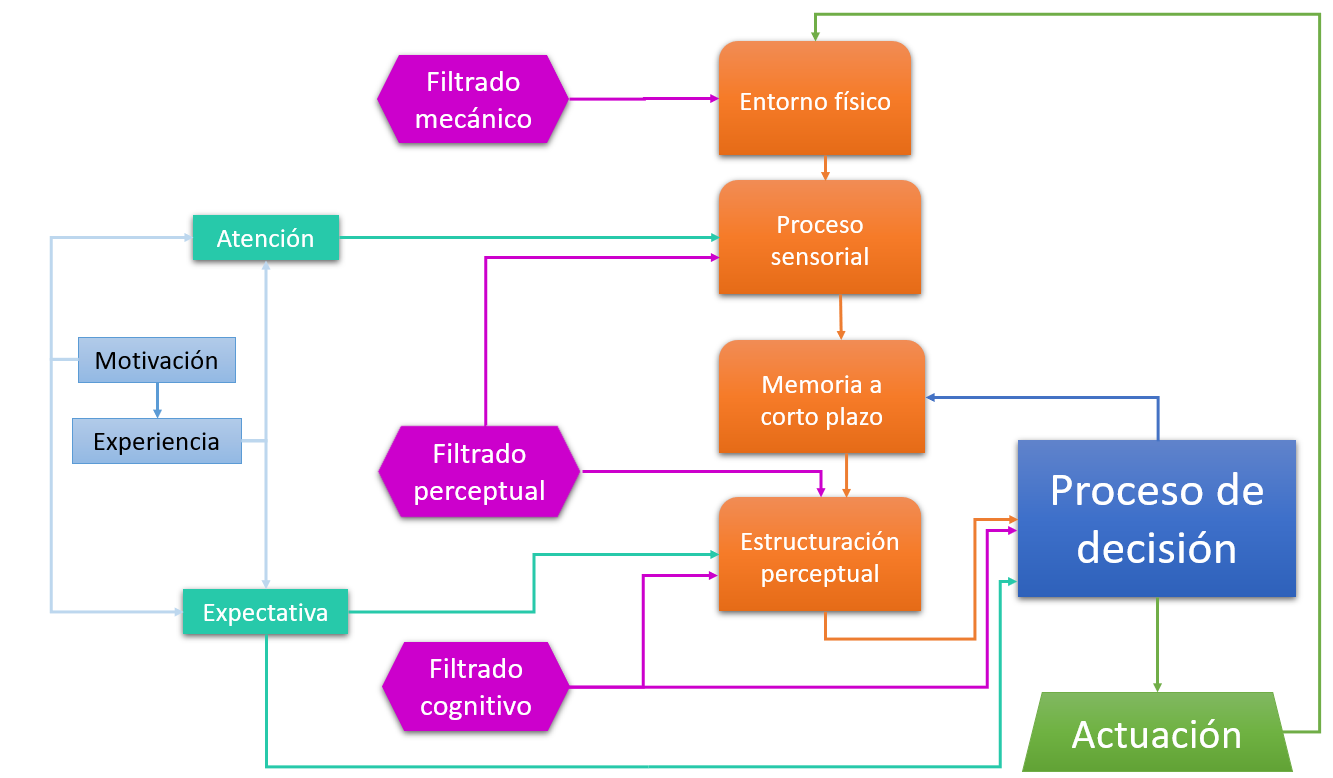
\includegraphics[width=12.5cm]{figures/1.1.png}
  \caption{\label{fig:1.1} Diagrama de las variables que intervienen en el proceso de decisión.}
\end{figure}

Estudiar el comportamiento del conductor proporciona información relevante en los procesos cognitivos empleados en la realización de una tarea, como son el orden de prioridades en el análisis del entorno, los tiempos de respuesta o los recursos mentales disponibles frente a estímulos. Es por ello por lo que numerosas empresas de vehículos con opciones de conducción parcialmente automatizada, se sienten abiertas a instalar sensores hacia el interior del habitáculo, con objeto de comprobar la atención del conductor en caso de aparecer un evento crítico. Numerosos fabricantes ya implementan sistemas basados en cámaras para detectar estados de somnolencia y fatiga, como Ford (Monitoring System), Toyota (Driver Monitoring System), Volkswagen (Fatigue Detection System), Mercedes-Benz (Attention Assist) y Volvo (Driver Alert Control) entre otros. La importancia de estos sensores reside en los primeros niveles de autonomía, donde el conductor es el principal supervisor y tiene la responsabilidad de retomar el control cuando la situación lo requiera. En la misma línea se observa que los procesos automatizados suelen derivar en un exceso de confianza por parte del supervisor, produciendo fenómenos como la hipovigilancia y el amodorramiento, que pueden ser evitables gracias a estos sensores. 

El dilema en la determinación de un evento crítico es el tiempo que invierte el sistema en identificarlo y darle el control al conductor. Una alta capacidad de cálculo en la detección debe complementarse con una buena identificación. A pesar de que los conductores humanos no son tan rápidos como un algoritmo matemático, este podría predecir un peligro con mayor antelación, valorando otros criterios no matemáticos y siendo el tiempo final de respuesta menor. Algunos algoritmos de toma de decisiones están basados en inteligencia artificial, con el fin de replicar las capacidades humanas de decisión. Sin embargo, no son capaces de crear razonamientos en base a situaciones que no se hayan definido previamente. Garantizar el máximo de reglas en el sistema de decisiones es determinante para poder tener un buen sistema de navegación.  

La caracterización del comportamiento del conductor es una parte importante en el desarrollo de los algoritmos de conducción, tanto a nivel individual como grupal. Las decisiones no solo dependen de variables espacio-temporales constantes, sino que la disposición del entorno y el comportamiento de los vehículos adyacentes pueden generar variabilidad en dichos parámetros. Además, una conducta eficiente y ordenada no es realista, ya que la conducción es un medio flexible, donde puede existir un lenguaje y una comunicación no verbal previa a la realización de ciertas maniobras. Debido a ello, un vehículo autónomo en tráfico mixto podría enfrentarse a situaciones de inadaptabilidad, al no comprender las intenciones de los demás vehículos o realizar acciones inesperadas. 

La comprensión de las decisiones humanas puede ser estudiada mediante el sistema visual, ya que es uno de los principales receptores de información relevante del entorno. Los movimientos oculares, al igual que el de la cabeza, son un reflejo de la estrategia atencional seguida, permitiendo determinar patrones en la ejecución humana de ciertas maniobras. Estudiar el proceso de resolución humano ante una situación demandante contribuye directamente a una mejora en la identificación de eventos críticos y a la elaboración de reglas en el sistema de decisión. En esta Tesis Doctoral se propone analizar la influencia de la complejidad del entorno sobre las variables atencionales del conductor, con el fin de elaborar algoritmos de toma de decisiones naturalistas que ayuden a la integración de la conducción autónoma en el tráfico mixto. 

\section{Objetivos}

El objetivo de esta Tesis se centra en aportar una solución a la integración de los vehículos autónomos en el tráfico mixto, a través de una mejora en la caracterización del comportamiento del conductor. La optimización del proceso de toma de decisiones, sobre el que se asientan los algoritmos implementados en vehículos autónomos, contribuye directamente en la resolución de situaciones imprevistas durante la conducción. Por ello, el objetivo principal es comprender la interpretación del entorno por parte de un conductor humano y desarrollar un modelo de toma de decisiones para vehículos autónomos a partir de esa interpretación. Observando las variables atencionales se puede determinar la estrategia atencional seguida, contribuyendo en el desarrollo de algoritmos de toma de decisiones naturalistas.

Al mismo tiempo se alcanzan los siguientes objetivos secundarios, los cuales son abordados en los tres capítulos que comprenden esta Tesis:

\begin{itemize}
  \item Analizar la influencia de las variables atencionales en maniobras complejas en vías de alta capacidad, como son autovías y autopistas, y el comportamiento del conductor ante diferentes niveles de asistencia en la conducción autónoma.
  \item Integrar el sistema de percepción del conductor con la fusión sensorial de detección del entorno, utilizando tecnologías de seguimiento ocular, láser 3D y visión artificial.
  \item Proponer, ajustar y validar un modelo determinista para la toma de decisiones aplicado a la conducción autónoma en base a diferentes niveles de información disponible. 
\end{itemize}

Las maniobras propuestas se resumen en incorporaciones, cambios de carril y adelantamientos, diferenciándose estas dos últimas en el rebase del vehículo delantero. Todos los ensayos experimentales se realizan en tráfico real, en contextos interurbanos, utilizando vehículos equipados con tecnología propia de la conducción autónoma. 

\section{Estructura de la tesis}

La presente Tesis Doctoral se estructura en los siguientes capítulos, como se describe a continuación.

El \hyperref[ch1]{Capítulo 1} corresponde a estas primeras páginas, sirviendo como \emph{Introducción} a dicho escrito y presentando las motivaciones y los objetivos que se pretenden alcanzar en esta investigación.
El \hyperref[ch2]{Capítulo 2} presenta el \emph{Estado de la cuestión}, mostrando mediante literatura los desarrollos existentes sobre los que se apoya la presente Tesis. Partiendo de los modelos de comportamiento existentes en la conducción se profundiza en las variables habitualmente utilizadas y los sensores a través de los cuales pueden ser obtenidas. Los desarrollos y las aportaciones de la Tesis Doctoral se presentan en los capítulos 3, 4 y 5. 
En el \hyperref[ch3]{Capítulo 3} se plantea la utilización de \emph{Variables atencionales} en la conducción, en concreto en los modelos de toma de decisiones. Se muestran dos apartados principales, concernientes a las maniobras de incorporación y adelantamiento en niveles de conducción parcialmente automatizada, donde se estudia la información proporcionada por el sistema de seguimiento visual en relación al estado del conductor y las estrategias atencionales empleadas en la realización de la maniobra. 
En el \hyperref[ch4]{Capítulo 4} se realiza una \emph{Fusión sensorial} entre el sistema de percepción del conductor, compuesto por el de seguimiento visual y el de captación del movimiento de la cabeza, y dos sistemas de percepción del entorno, constituidos por una cámara y un sensor láser, determinando los obstáculos que el conductor mira durante la conducción. 
El \hyperref[ch5]{Capítulo 5} propone el desarrollo de un algoritmo para un \emph{Modelo de toma de decisiones en conducción autónoma} con objeto de mejorar el naturalismo de los modelos de comportamiento. Este capítulo se completa con los resultados obtenidos de los capítulos anteriores, gracias a los cuales el modelo será ajustado y validado utilizando datos de ensayos experimentales en conducción real.
Por último, se presentan las \hyperref[ch6]{Conclusiones y líneas de investigación futuras} junto a la \hyperref[ch7]{Difusión de resultados} en revistas y congresos de índole nacional e internacional concernientes a la Tesis Doctoral. 



\makechapter{Estado de la cuestión}{Estado de la cuestión}{Estado de la cuestión\label{ch2}}
En este capítulo se presentará una revisión exhaustiva de la literatura existente relacionada con la toma de decisiones en conducción autónoma. A través de investigaciones previas relacionadas con la temática, se expondrá el estado actual y los retos que plantean los vehículos autónomos, desde investigaciones que abordan desde una perspectiva global hasta trabajos más específicos relacionados con la información adquirida por los sensores.

\section{Vehículos autónomos: actualidad y desafíos}

La seguridad en la industria del automóvil es uno de los temas que más preocupa a la sociedad actual. A pesar de los avances tecnológicos realizados en las últimas décadas, los accidentes de tráfico se siguen considerando una de las principales causas de muerte en todo el mundo, con proyección de aumentar en un futuro próximo (\cite{who2018}). El último estudio publicado por la Agencia Nacional de Seguridad Vial Americana, en inglés \gls{nhtsa}, reveló que la principal causa de los siniestros graves es el factor humano, en el cual se engloban errores como el reconocimiento, la decisión y la ejecución principalmente (\cite{nhtsa18}). 

Los vehículos autónomos proyectan un futuro más seguro y confiable para los conductores, paliando los problemas derivados de la conducción manual y descargando al conductor del procesamiento de información. El desarrollo de la conducción autónoma posee muchas ventajas que benefician a la sociedad como son la reducción de la siniestralidad, la liberación de espacios dedicados a aparcamientos, el compromiso medioambiental y la nueva gestión del tiempo dedicado a la conducción (\cite{terrones}). Para entender su campo de actuación es necesario explicar los niveles en los que se dividen y sus funciones. En 2014, la \gls{sae} estableció seis niveles de automatización, del 0 al 5, los cuales comprendían desde la conducción manual hasta la automatización total. 

En abril de 2021 se realiza la última actualización de dicha clasificación, donde se perfecciona la separación entre los niveles 3 y 4 y se extienden los primeros niveles ajustándose a los avances desarrollados (\cite{sae}). En la figura \ref{fig:2.1} se muestra un esquema proporcionado por \gls{sae} con las características de cada nivel adaptado al español.

\newpage
\begin{figure}[htb]
  \centering
  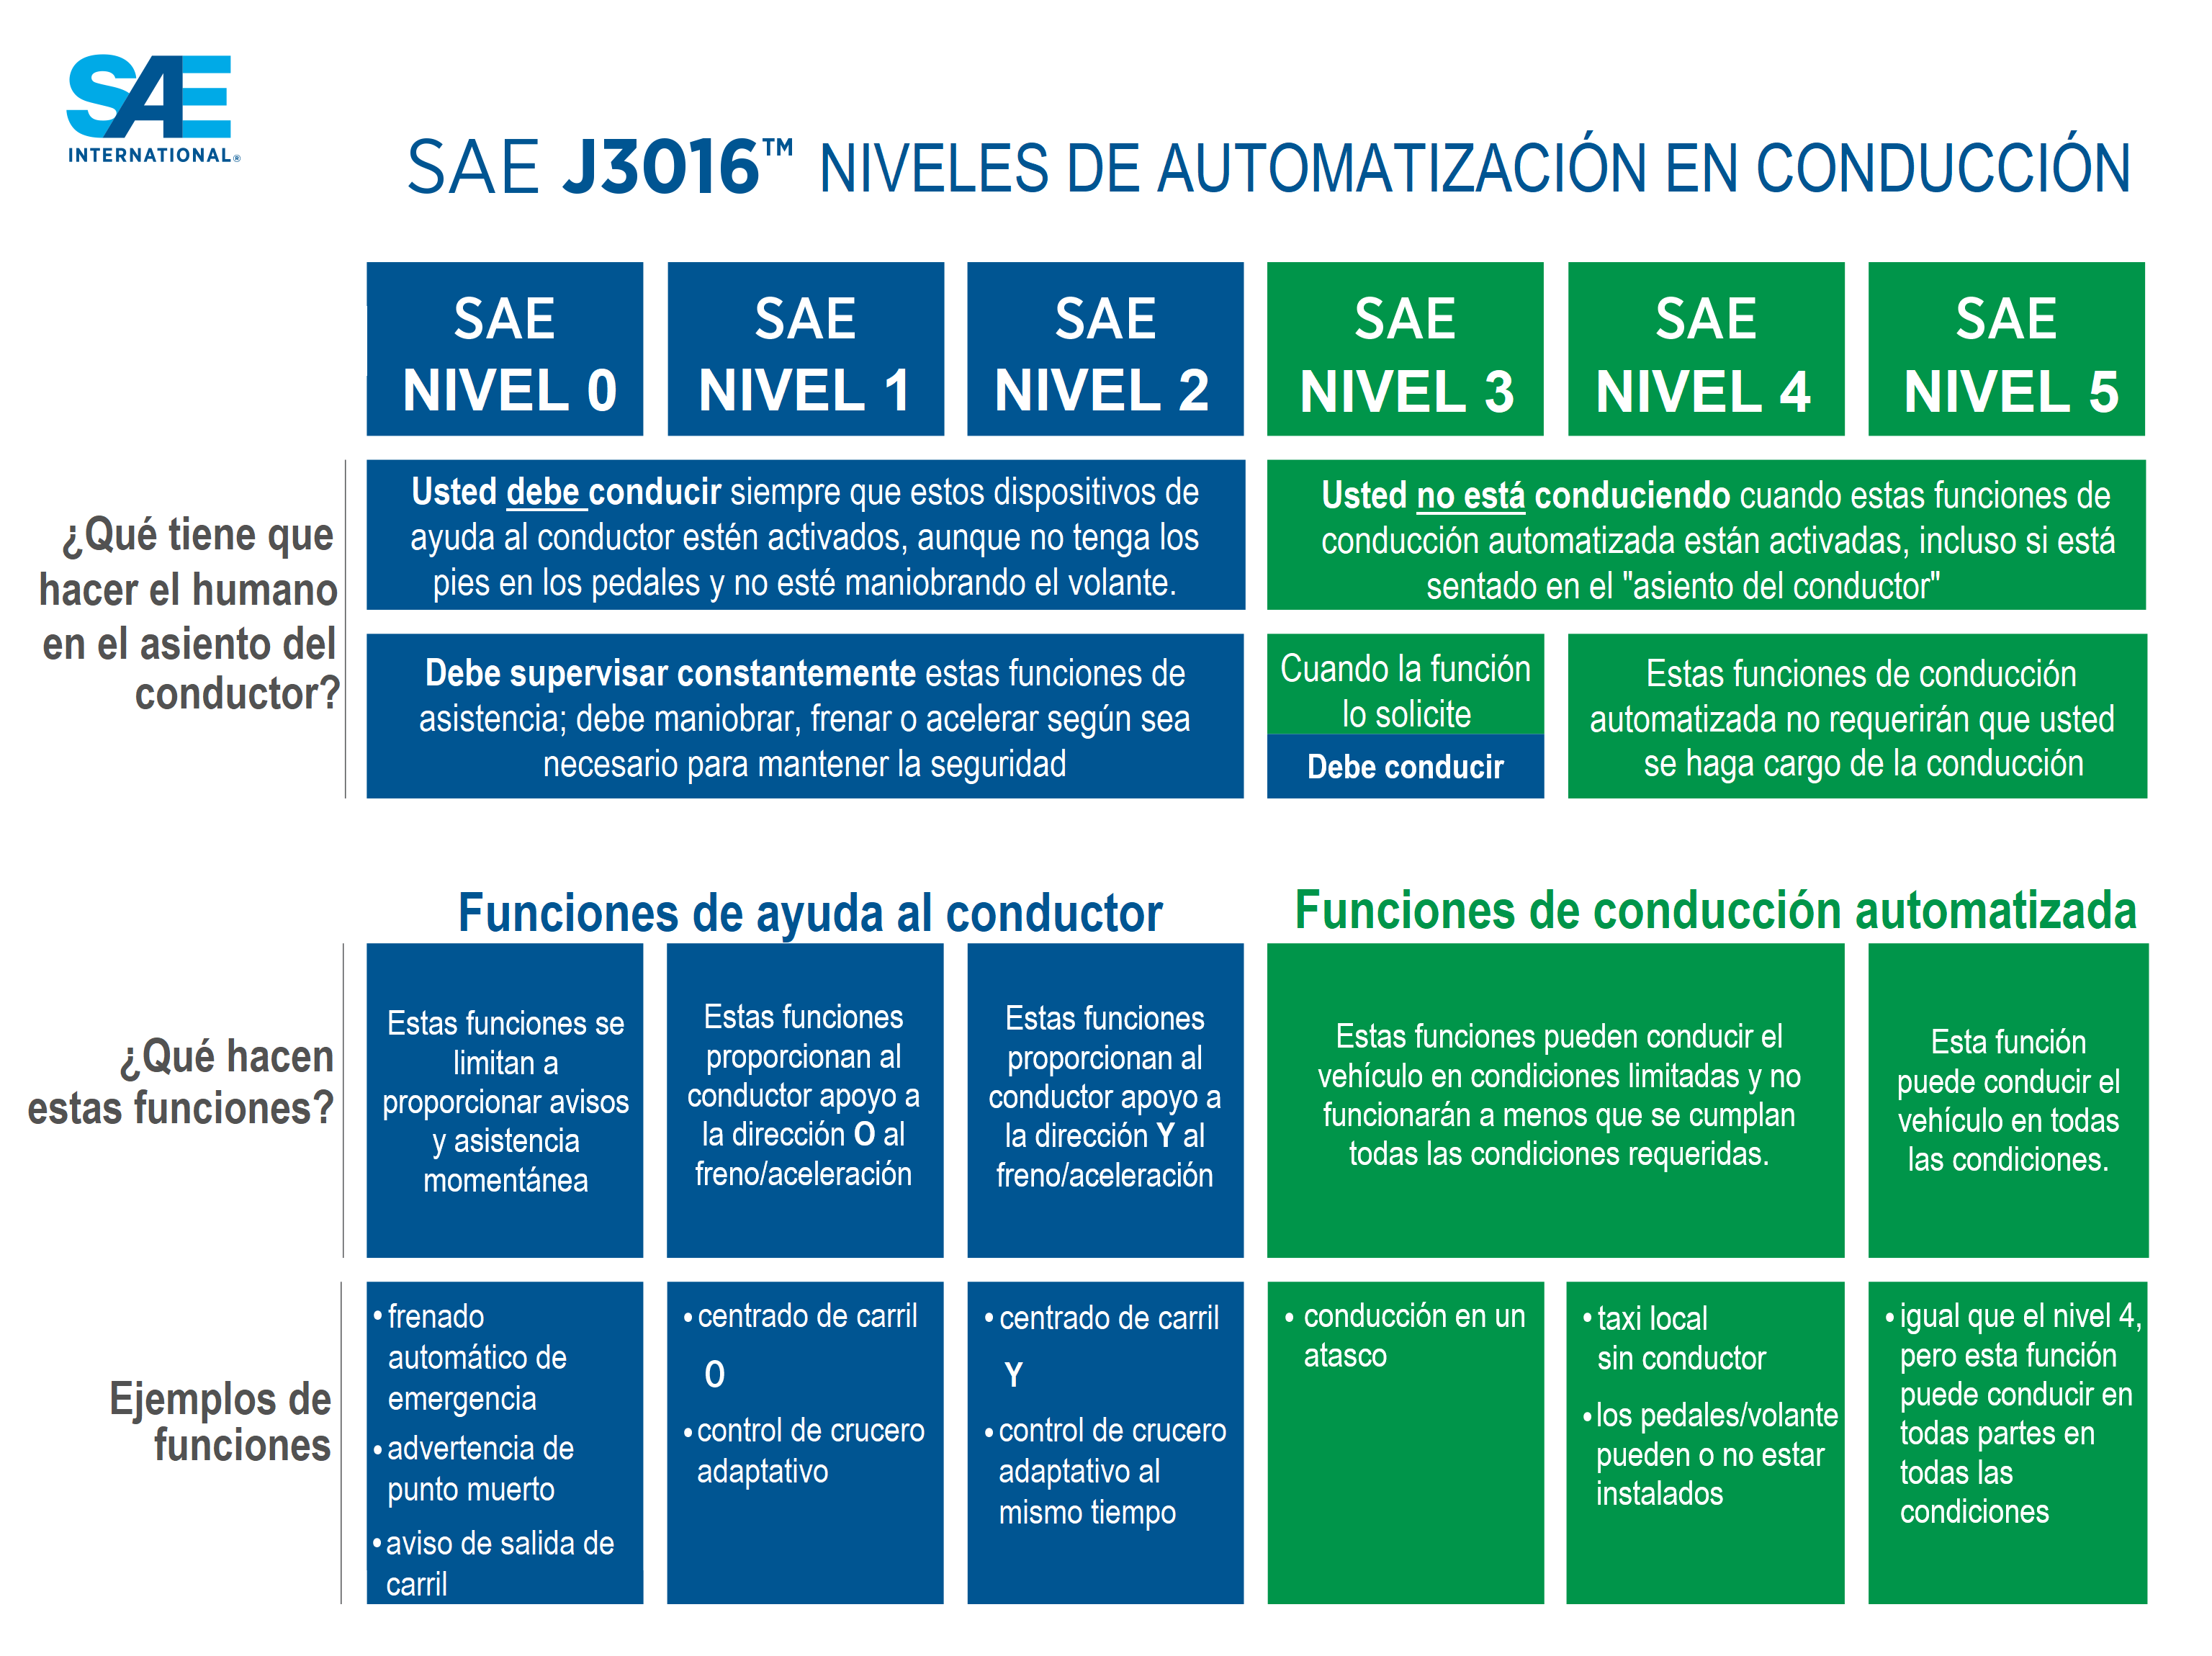
\includegraphics[width=13.5cm]{figures/2.1.png}
  \caption{\label{fig:2.1} Niveles de automatización en conducción (original en \textcite{sae}).}
\end{figure}

De igual manera, en junio de 2022 la \gls{nhtsa} publicó unos informes sobre accidentes relacionados con la conducción autónoma a lo largo de un año, gracias a los reportes proporcionados por los fabricantes de vehículos en diferentes niveles de automatización. Estos resultados aportan transparencia sobre la seguridad de dichos vehículos y proporcionan datos importantes para la investigación y para el desarrollo de políticas que mejoren la seguridad en estas tecnologías. A pesar de que dichos resultados son poco representativos, debido a la naturaleza de la muestra, permiten vislumbrar unos primeros resultados a nivel proporcional. Los informes se dividen en dos, accidentes para vehículos hasta nivel 2 equipados con sistemas avanzados de asistencia al conductor, en inglés \gls{adas} (\cite{nhtsa22a}) y accidentes para vehículos en los niveles 3-5 de automatización (\cite{nhtsa22b}). 

Los fabricantes que más datos reportaron fueron Tesla y Honda para vehículos hasta nivel 2, y Waymo y Transdev para niveles superiores de automatización. Las colisiones con otros vehículos de la vía, fueron alrededor de un 30\% para vehículos hasta nivel 2 y un 80\% para el resto de niveles, notándose los problemas actuales de integración de la conducción altamente automatizada con el tráfico mixto (Figura \ref{fig:2.2} y Figura \ref{fig:2.3}). 

\newpage
\begin{figure}[h]
  \centering
  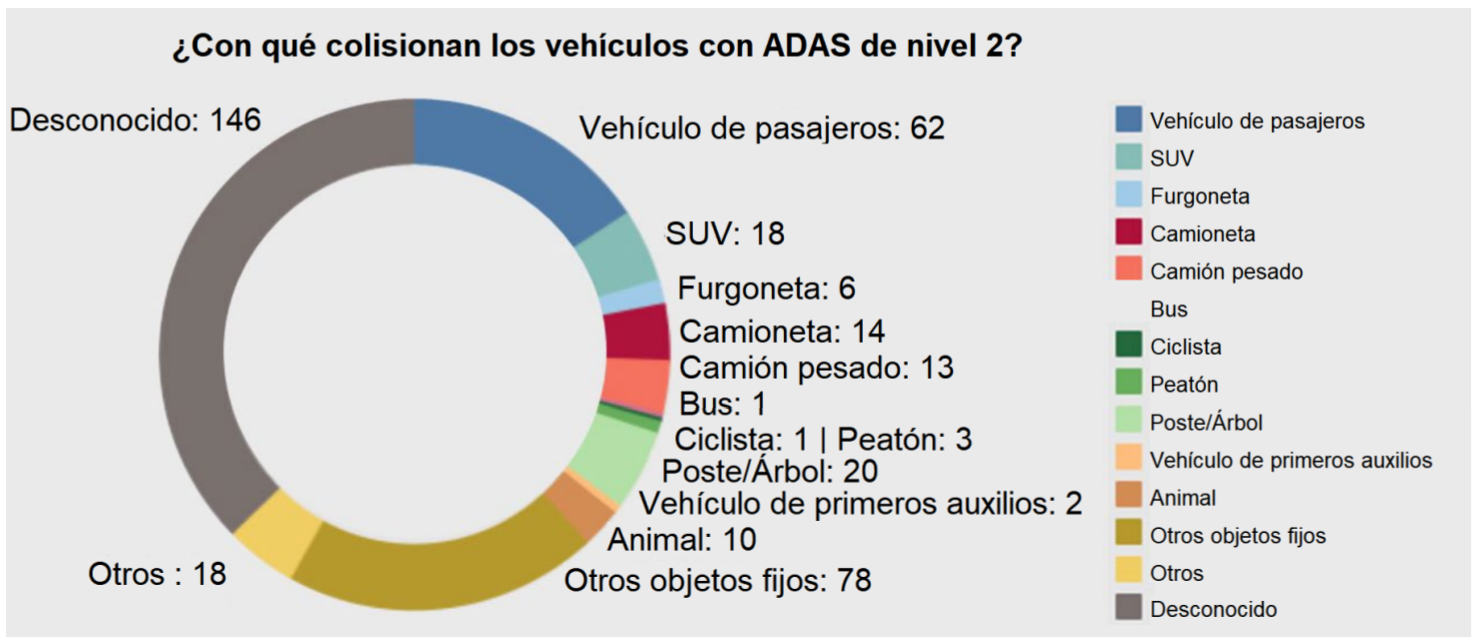
\includegraphics[width=12.5cm]{figures/2.2.png}
  \caption{\label{fig:2.2} Colisiones de vehículos autónomos con \gls{adas} de nivel 2 (original en \textcite{nhtsa22a}).}
\end{figure}

\begin{figure}[h]
  \centering
  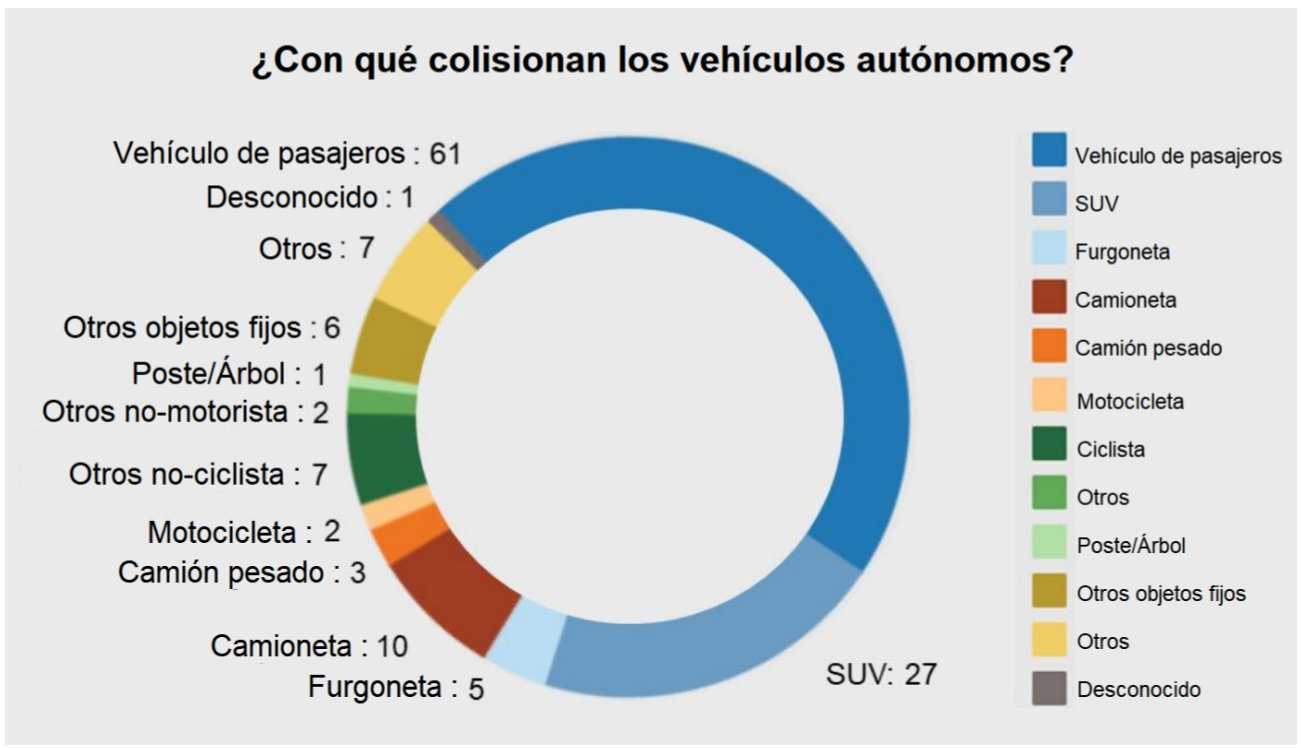
\includegraphics[width=10.5cm]{figures/2.3.png}
  \caption{\label{fig:2.3} Colisiones de vehículos autónomos en niveles 3-5 (original en \textcite{nhtsa22b}.}
\end{figure}

Los principales daños para vehículos de niveles inferiores fueron en la parte frontal del vehículo (frontal, seguido de frontal-izquierdo y frontal-derecho), todo lo contrario que los vehículos de niveles superiores, donde los daños se produjeron especialmente en la parte trasera (trasera, seguido de trasera-izquierda y trasera-derecha).
El conjunto de los resultados permite discernir que en la conducción automatizada existen diferentes modos de conducción y que, por tanto, los problemas que puedan surgir en cada uno de los niveles deben de estudiarse independientemente. Los alcances frontales para los vehículos equipados con \gls{adas}, donde es necesaria la intervención del conductor, sugieren que una confianza excesiva en el sistema, que repercute en una falta de atención y una reacción tardía del conductor ante un evento inesperado (\cite{cunningham}; \cite{yang21}; \cite{mcwilliams}; \cite{hsieh}). Por contra, en los vehículos altamente automatizados los daños traseros se podrían relacionar con frenadas bruscas, que apuntan a un problema de error de percepción, donde se detectan obstáculos que no existen, denominado comúnmente como falsos positivos (\cite{bellosalau}; \cite{buhler}; \cite{zhang22}). Estas dos hipótesis han sido ampliamente estudiadas por la comunidad científica, como se observa en los siguientes apartados, abriendo un abanico de líneas de investigación para cada una con objeto de mejorar la conducción autónoma en todas sus facetas.

\subsection{Conducción parcialmente automatizada}
En los últimos años, la industria del automóvil ha contribuido al desarrollo de distintos dispositivos de protección para mejorar la seguridad en la conducción, desde el cinturón de seguridad hasta los sistemas de ayuda a la conducción. A través de esta tecnología es posible controlar y limitar factores tan importantes como el entorno o el error humano, asistiendo al conductor en la toma de decisiones y recomendándole medidas ante situaciones potencialmente peligrosas (\cite{schoegg}). Estos sistemas cobran especial importancia en los niveles 1 y 2, encargándose del control de bajo nivel, ya sea parcial o totalmente. La presencia de sensores de percepción del entorno como cámaras, radares o láseres, entre otros, permiten que el vehículo ejecute ciertas acciones básicas de forma independiente, pero siempre con la supervisión del conductor. Sin embargo, estos primeros niveles son sensibles a una mala praxis por parte del conductor, ya que se enfrenta a una forma diferente de conducir, donde físicamente podría abandonar alguno de los controles, pero cognitivamente no puede salir el bucle de control. Estudiar su comportamiento es fundamental para el desarrollo y la implementación de sistemas funcionales cuyo fin sea mejorar la seguridad en carretera. 

En este punto, se encuentran estudios sobre la interacción con sistemas de ayuda en conducción parcialmente automatizada que abordan problemas como el rendimiento en la realización de tareas secundarias (\gls{ndrt}), la atención dividida en la monitorización del entorno y la recuperación de la toma de control del vehículo (\cite{naujoks16}; \cite{solismarcos}; \cite{hensch}; \cite{zangi}; \cite{li22a}). La activación de sistemas de ayuda a la conducción reduce la frecuencia de eventos y estímulos para el conductor, incitándole a la realización de tareas distractoras y dando lugar a una monitorización pasiva del entorno (\cite{endsley}). Este hecho compromete la seguridad de la conducción ya que derivaría en una anticipación deficiente ante la aparición de un evento crítico. La falta de atención o las distracciones son elementos a evitar en cualquier tipo de conducción, debido a que suponen un gran porcentaje de las colisiones que se producen en tráfico real como se expone en \textcite{neale}, donde el 78\% de las colisiones y el 65\% de las casi colisiones se debían a esta causa.

No obstante, se encuentran aportaciones interesantes que plantean soluciones constructivas en este asunto. En \textcite{lee19} se observó que el efecto de entablar una conversación disminuye significativamente la fatiga y el aburrimiento del conductor generado por la automatización en el nivel 2 de su vehículo. Numerosos autores se apoyan en analizar el comportamiento visual del conductor para obtener resultados sobre la carga mental que suponen estas situaciones y posibles mejoras en el diseño para favorecer las capacidades del conductor (\cite{forster}; \cite{chen}; \cite{ulahannan}; \cite{goncalves}). Este conocimiento ayuda a la caracterización del conductor, la cual se debe de contemplar dentro de los algoritmos de control del vehículo, facilitando la maniobrabilidad del conductor y evitando problemas derivados de la falta de atención y las distracciones (\cite{ahlstrom}; \cite{cunningham}). Aunque estos dilemas estén más presentes en la conducción parcialmente automatizada, también son aplicables a niveles superiores de automatización donde se requiera la intervención del conductor ante un evento crítico (\cite{jimenez18}; \cite{morales}; \cite{merlhiot}).

\subsection{Conducción altamente automatizada}
La realidad que parece más cercana es la conducción parcialmente automatizada, implementando poco a poco cada uno de los niveles de automatización en la sociedad actual. Sin embargo, existen vertientes que sugieren que el éxito del vehículo autónomo reside en particularizar el entorno por el que circule, eludiendo la problemática que entraña el tráfico mixto (\cite{ma}; \cite{zhang20}). La creación de un carril específico para vehículos altamente automatizados beneficiaría tanto a los usuarios como a los demás vehículos del entorno, eliminando la necesidad de un conductor y estableciendo un transporte tan seguro como el tren o el metro. De esta manera, se promovería la confianza en la tecnología de conducción autónoma y se reduciría la probabilidad de accidentes causados por errores humanos (\cite{nickkar}; \cite{zhang20}; \cite{sohrabi}). Sin embargo, esta solución puede alterar la capacidad de la vía debido al aumento del flujo de tráfico en caso de no tener espacio suficiente para la creación de este carril exclusivo (\cite{ghanipoor}; \cite{santana}).

A pesar de que los vehículos altamente automatizados prometen una mayor seguridad en la carretera al reducir los errores humanos, la convivencia con los vehículos convencionales en el tráfico mixto puede implicar ciertas complicaciones debido a la interacción entre los mismos. Relacionado con ello, los autores \textcite{favaro} y \textcite{petrovic} analizaron una base de datos de accidentes donde estuvieron involucrados vehículos con algún grado de autonomía. Entre los vehículos analizados destacaron los niveles de autonomía 4 y 5, ya que la empresa Waymo reportó la mayor cantidad de informes, debido a su mayor flota y kilometraje recorrido en comparación con otros fabricantes. En ambos estudios se obtuvo que las colisiones traseras con un vehículo convencional fueron el accidente más frecuente, señalando a un posible error humano causado por una conducción demasiado cercana al vehículo delantero o una velocidad insegura. Dinámicamente, los vehículos autónomos se comportan diferente a los convencionales, lo cual puede resultar confuso para un conductor humano cuyo concepto de velocidad y aceleración no es tan suave y gradual. En el estudio de Petrović se sugiere la colocación de una señal en la parte trasera del vehículo que indique que se trata de un vehículo autónomo, con objeto de advertir sobre la posibilidad de que presente acciones imprevistas. Además, destaca la importancia de educar a la población sobre las características de los vehículos autónomos en la circulación del tráfico, lo que aumentaría la conciencia sobre las diferencias en las características dinámicas entre los mismos. En este contexto, es importante tomar medidas para mejorar la seguridad en la carretera y aumentar la conciencia sobre las características de los vehículos autónomos.

La confiabilidad de los conductores en vehículos de alta automatización depende en gran medida del riesgo percibido (\cite{li19}) al igual que de la información proyectada por el vehículo mientras está operando en modo autónomo (\cite{danner}). Sin embargo, esta variable puede verse afectada negativamente por la aparición de falsos alarmas en la detección de obstáculos, generando una disminución de la confianza en el sistema debido a la percepción de un nivel de riesgo superior al real (\cite{drexler}). Debido a esto, es necesario el desarrollo de algoritmos precisos capaces de detectar y caracterizar la mayor variedad de anomalías posibles que puedan ocurrir durante la conducción (\cite{bellosalau}). 

\section{La toma de decisiones en conducción autónoma }
Uno de los procesos más importantes en el desarrollo de un vehículo autónomo es el proceso de la toma de decisiones. Los vehículos procesan la información recopilada por los sensores con objeto de identificar obstáculos y situaciones críticas en la carretera, analizando las posibles opciones para determinar la opción más segura. Este proceso se basa en modelos matemáticos, diseñados para imitar la manera en que los conductores responden a diferentes situaciones del entorno. Para poder entender la complejidad de los algoritmos de toma de decisiones es necesario conocer en detalle la base de los modelos de comportamiento del conductor.

\subsection{Modelos de conducción}
La tarea de conducción se puede dividir en dos movimientos principalmente, longitudinal y lateral. Para caracterizar cada una de estas acciones los primeros autores se refirieron a ellas como seguimiento de vehículo o car-following (\cite{reuschel}; \cite{pipes}) y cambio de carril o lane-changing (\cite{sparmann}; \cite{gipps}). Desde entonces, las técnicas de modelado han dado lugar a múltiples desarrollos interesantes que son referencia en los modelos de conducción (\cite{chandler}; \cite{herman59}; \cite{newell}; \cite{gazis}; \cite{bexelius}; \cite{ahmed96}; \cite{halati}; \cite{toledo03}). Numerosas revisiones, entre ellas \textcite{brackstone}, \textcite{olstam} y \textcite{diaz}, analizan su evolución diferenciando cada una de las vertientes propuestas por los autores. 

Ambas acciones han de analizarse en conjunto ya que, de manera general, la maniobra de cambio de carril tiene su inicio en un ajuste de velocidad respecto al vehículo que le precede. Los criterios en la toma de decisiones durante este proceso han suscitado diversas teorías para predicción del comportamiento del conductor. Una de las más populares es la aceptación de huecos o gap-acceptance, la cual se estudia en las publicaciones de \textcite{herman61}, \textcite{drew} y \textcite{miller}, en diferentes distribuciones. Factores como el tipo de cambio, la velocidad del líder, la distancia hasta al final del carril, la cooperación entre vehículos, los huecos rechazados y el tiempo de espera dieron paso a numerosos estudios en el análisis de su ejecución (\cite{mahmassani}; \cite{gipps}; \cite{madanat}; \cite{cassidy}; \cite{ahmed96}; \cite{yang96}; \cite{halati}; \cite{hidas}; \cite{toledo07}).

\begin{figure}[h]
  \centering
  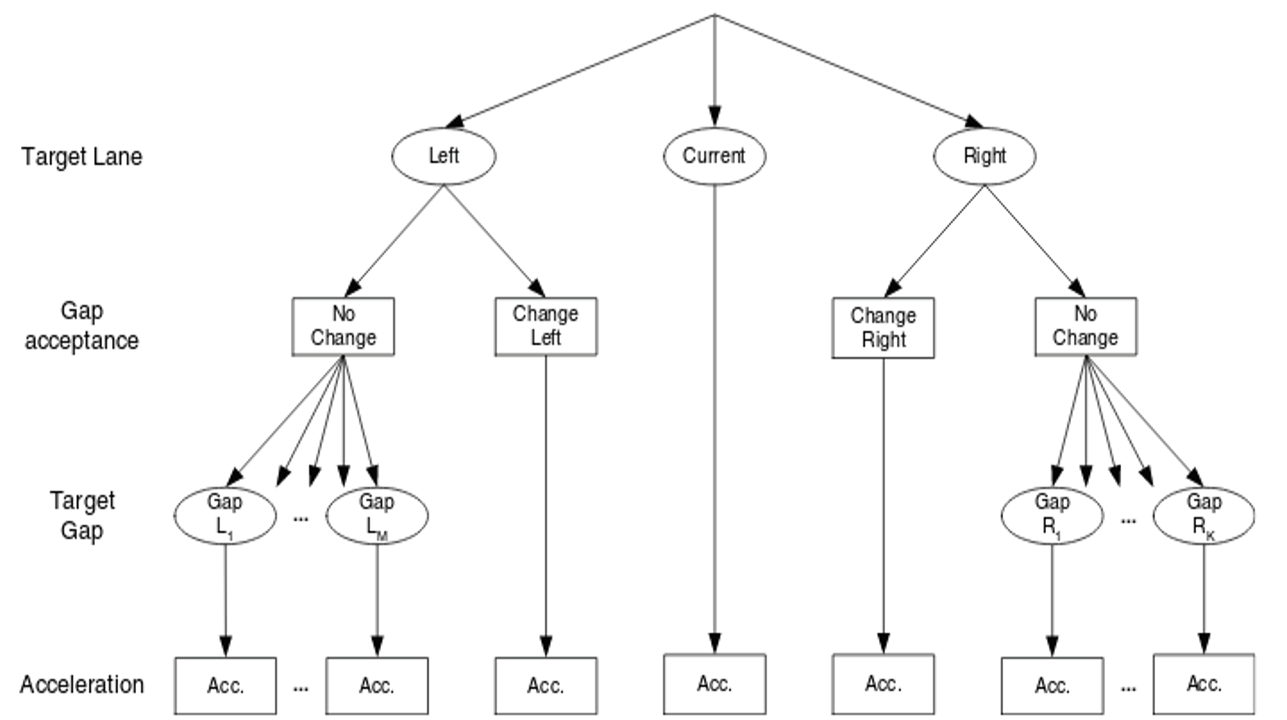
\includegraphics[width=12.5cm]{figures/2.4.png}
  \caption{\label{fig:2.4} Estructura del modelo de comportamiento de los vehículos (\cite{toledo07}).}
\end{figure}

El comportamiento del conductor no adquirió naturalismo hasta la aparición de los modelos psicofísicos (\cite{michaels}; \cite{wiedemann74}) que daría pie a una nueva línea de modelos donde se contemplasen variables cognitivas dando lugar a modelos más predictivos y realistas. Posteriormente el trabajo realizado por \textcite{michon} introdujo los procesos cognitivos en el análisis de las tareas de conducción, dividiendo la tarea en tres niveles jerárquicos, el estratégico, el táctico y el de control, situándose la toma de decisiones en el segundo nivel.

Dado que el entorno y el estado del conductor influyen directamente en las acciones que realiza, se establecieron subdivisiones dentro de los movimientos principales de la conducción llamados regímenes. Ejemplo de ello es la investigación publicada por \textcite{wiedemann92}, donde se presentó un modelo psicofísico de seguimiento de vehículo definido por diferentes regímenes de aceleración (aceleración libre, seguimiento de vehículo, acercamiento y emergencia). En \textcite{sharma19} se identificaron hasta seis regímenes diferentes para completar una trayectoria, definidos como aceleración, aceleración libre, seguimiento, crucero, desaceleración y parada. 

Por otro lado, los modelos de predicción también son clasificados según sus características conceptuales, diferenciando entre modelos deterministas, cuya ventaja principal es que son más fáciles de desarrollar y sus resultados son repetibles, y los modelos estocásticos, que incluyen  procesos aleatorios pudiendo abarcar muestras de gran tamaño y contemplando incertidumbres significativas. En ambos planteamientos se han realizado estudios interesantes, como es el caso de \textcite{vanbrummelen}, donde se desarrolló un modelo probabilístico al estacionamiento de un vehículo aplicado a la conducción autónoma. En predicción probabilística se encuentran diversos trabajos relacionados con el proceso de decisión de Markov, en su forma oculta y parcialmente observable, en el campo de la conducción autónoma (\cite{guan}; \cite{park}; \cite{li21a}). Pero la diversificación de estas metodologías no incluye su división, ya que en estudios muy recientes (\cite{suh}, \cite{luo}) se propusieron modelos predictivos fusionando el enfoque determinista y probabilista para la decisión de cambio de carril en conducción autónoma.

\subsection{El proceso de decisión en algoritmos naturalistas}

En la conducción autónoma, la toma de decisiones es fundamental para asegurar un desplazamiento seguro y eficiente. En el contexto del tráfico mixto, la comunicación entre vehículos autónomos y vehículos conducidos por humanos debe ser lo más análoga posible, evitando situaciones confusas que puedan derivar en malentendidos o accidentes (\cite{jenssen}). Por ello, la capacidad de comprender las intenciones de otros vehículos se convierte en una tarea fundamental para el vehículo autónomo. Aunque esta habilidad sea característica de un conductor real, los algoritmos de percepción y toma de decisiones deben ser capaces de comprender y anticipar las acciones humanas para garantizar una conducción confiable. De igual manera, la respuesta del vehículo autónomo debe ser adecuada y comparable a la que realizaría cualquier conductor en el mismo entorno, con objeto de que los demás vehículos puedan advertir claramente sus intenciones. 

Para lograr una respuesta adecuada del vehículo autónomo, es importante tener en cuenta la caracterización del conductor y el análisis de su comportamiento frente a diversas situaciones, tanto cotidianas como complejas. Sin embargo, la comprensión completa de los factores humanos y los procesos de toma de decisiones durante la conducción debe de ser contemplada desde un enfoque interdisciplinar y colaborativo, incluyendo profesionales del sector de la ingeniería, la psicología y la industria del transporte (\cite{cacciabue}). Los desarrollos de toma de decisiones basados en conducción naturalista abordan este problema mediante la identificación de patrones y reglas de comportamiento de los conductores a través de datos adquiridos de situaciones reales. La información es recogida de los sensores ubicados en el vehículo y el propio conductor, procediendo bien del posicionamiento del vehículo, como son acelerómetros, giróscopos o sistemas de posicionamiento; del entorno exterior, englobando los sistemas radar, los sistemas de detección y medición de distancias por luz, en inglés \gls{lidar} y las cámaras; o de la fisiología del conductor, evaluando su comportamiento visual, actividad cerebral o respuestas físicas. La toma de decisiones naturalista ha sido ampliamente estudiada, siendo su principal foco la caracterización de maniobras en entornos complejos, como son rotondas (\cite{cuenca}; \cite{kong}), cambios de carril (\cite{yang19}; \cite{shawky}; \cite{ali21}) e incorporaciones a una vía principal (\cite{kang}; \cite{gu}). Los estudios naturalistas pueden generar grandes volúmenes de información que permiten extraer patrones concretos de conducción a través de la observación de variables. Analizando estos datos es posible construir modelos que describan de forma estadística la realización de determinadas maniobras durante la conducción (\cite{bender}), extrayendo información del entorno o del propio conductor. 

Por otro lado, también se encuentran repositorios muy completos donde se analizan variables fisiológicas del conductor, como es el movimiento de los ojos y de la cabeza, para perfeccionar la determinación de un cambio de carril (\cite{deng}). En la investigación desarrollada por \textcite{xia}, se hace referencia al mecanismo de atención selectiva del sistema de visión humana para crear un modelo de intención de cambio de carril naturalista. En otros estudios de la misma índole, se analiza la actividad cerebral de los conductores para la modelización de su comportamiento en la realización de rotondas (\cite{monsalve}). Centrado en el vehículo autónomo, los patrones visuales aportan información sobre el estado de desconexión de un conductor durante el uso del piloto automático de un vehículo Tesla (\cite{morando}), elaborando un modelo basado en datos de conducción naturalista a través de diferentes sensores, tanto exteriores como interiores al vehículo. De igual forma, los sistemas de ayuda a la conducción son comúnmente evaluados por sistemas de seguimiento visual (\cite{sanchez}; \cite{azevedo}; \cite{schindler}; \cite{zhou}), los cuales aportan información relevante sobre su diseño y operatividad.

Enfatizando en los sistemas de seguimiento visual, es importante destacar su relación con las intenciones del conductor, ya que ayuda a la generación de reglas de decisión para la mejora de algoritmos de toma de decisiones. El comportamiento ocular de un conductor durante la exploración de una escena, puede ser una herramienta valiosa en el desarrollo de planificaciones previas al proceso de decisión. En \textcite{lappi} se realizó un estudio naturalista enfocado a la estrategia de la mirada del conductor, resumiendo en siete los objetivos mirados más relevantes, los cuales fueron la mirada a la carretera o al infinito, a los instrumentos y espejos retrovisores, a intersecciones, señalizaciones, elementos físicos de la carretera y a la propia escena global. Conocer las variables más importantes para el conductor es una cuestión fundamental en la elaboración del algoritmo de control para un vehículo autónomo cuyo entorno actual es el tráfico mixto. 

\subsection{Factores en el modelado del conductor}
La conducción es un proceso complejo que implica la consideración de múltiples factores, los cuales pueden afectar significativamente en el sistema decisión. La diversidad de variables es tan amplia que, ante un mismo entorno, se pueden tener soluciones totalmente opuestas. Por ello, es importante definir los parámetros que regirán el funcionamiento del modelo y tener en consideración los factores no contemplados con el fin de obtener resultados precisos y confiables.  

Numerosos autores han identificado parámetros importantes en el proceso de modelización (\cite{cacciabue}; \cite{hole}; \cite{saifuzzaman}; \cite{jimenez17}). En este último trabajo, Jiménez se llevó a cabo un análisis detallado de las distintas dimensiones que conforman los factores humanos en la conducción, presentando un mapa donde se muestran los diversos factores que influyen en el estilo de conducción, resumidos en factores humanos, ambientales y vehiculares (Figura \ref{fig:2.5}). 

\begin{figure}[h]
    \centering
    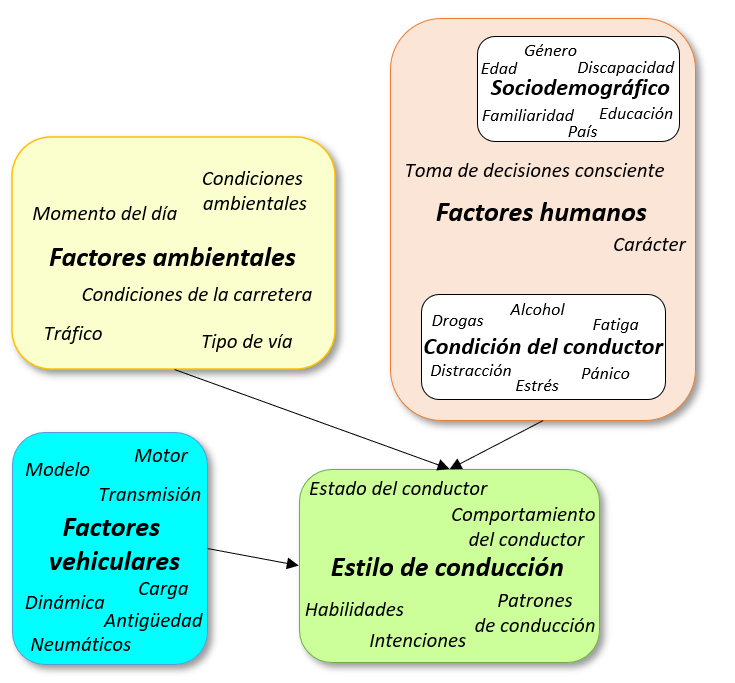
\includegraphics[width=10.5cm]
    {figures/2.5.png}
    \caption{ \label{fig:2.5} Factores relacionados con la conducción humana (original en \cite{jimenez17})}
\end{figure}

Por otro lado, en \textcite{bonsall} se estudian los parámetros relacionados con la seguridad en los modelos de simulación de tráfico, los cuales engloban submodelos de comportamiento relacionados con el seguimiento de vehículo, aceptación de huecos y cambio de carril. Los principales parámetros se resumen en velocidad y avance deseado, tasa de aceleración y deceleración, tiempo de reacción, hueco aceptable, crítico y mínimo en la realización de maniobras de cambio de carril.
Considerando los desarrollos propuestos en esta tesis, en los siguientes apartados se profundizará en los estudios previos relacionados con las variables de aceleración, deceleración, tiempo de reacción y hueco aceptable. La elección de unos valores óptimos y adecuados permitirá una modelización precisa del comportamiento del conductor y, por tanto, contribuirá en una mejora en el diseño de los algoritmos de conducción autónoma.

\subsubsection{2.2.3.1	Niveles de aceleración y deceleración}

La parametrización de un modelo de comportamiento del conductor implica considerar diversos factores, donde la dinámica longitudinal es uno de los más importantes. La capacidad de aceleración y deceleración del vehículo es un factor crucial en la definición de maniobras, sin embargo, su integración en un algoritmo de conducción no es una tarea fácil. En conducción real, estos parámetros son dependientes de las características del vehículo y el entorno que le rodea, como es el estado de la carretera o la suavidad con la que se realiza una maniobra, por lo que para cada situación es necesario contemplar un rango especifico. 

A diferencia de los niveles de deceleración, el estudio de los niveles de aceleración son un tema complejo, debido a su dependencia con la marcha en la que el vehículo se encuentra operando. No obstante, existen estudios que definen rangos de operación para aplicaciones donde es necesario definir unos límites de aceleración y frenado en el diseño de algoritmos de conducción. En \textcite{vanarem} se evaluó el impacto de un sistema de control crucero adaptativo a través de simulación, estableciendo unos valores de aceleraciones máximas confortables de 2 m/s$^2$ y -3 m/s$^2$, en aceleración y deceleración respectivamente. Sin embargo, para el mismo caso de estudio, en \textcite{yi} se consideró que este rango debería ser más estrecho, estando comprendido entre 1 m/s$^2$ a -2.5 m/s$^2$. Por otro lado, \textcite{prestl} estableció un intervalo de 1 m/s$^2$ a -2 m/s$^2$ en concepto de aceleraciones para el desarrollo de un sistema inteligente, con objeto de evitar problemas en el flujo del tráfico en caso de una decisión poco apropiada. 

En el estudio naturalista planteado por \textcite{danaher} se analizó el comportamiento del conductor en las diferentes fases de aceleración entre dos intersecciones, obteniendo valores de aceleración promedio de 0.12g para el primer segundo, 0.26g del segundo hasta el tercero, 0.22g hasta el quinto y 0.17g hasta el séptimo. En materia de desaceleración desde el pico máximo hasta su detención total obtuvo 0.19g desde el primer segundo hasta el sexto y 0.09g del sexto al octavo. La aceleración media en intersecciones señalizadas también fue objeto de investigación en \textcite{almallah} junto al tiempo de reacción y la sobreaceleración, obteniendo valores de 2.8 m/s$^2$ de media para la variable en cuestión.

En la actualización sobre la teoría del flujo de tráfico realizado por \textcite{gartner}, también se aborda el proceso de aceleración, considerando rangos nominales entre 0.6 m/s$^2$ y 0.7 m/s$^2$ para una aceleración confortable a velocidades a partir de 48 km/h. En situaciones donde los conductores circulan con urgencia, se encuentran valores superiores que llegarían a estar alrededor de 1 m/s$^2$. Estudios naturalistas más recientes, obtuvieron resultados similares a los anteriores en la evaluación de diferentes modelos de seguimiento de vehículos (\cite{he}), aunque también respaldan que los valores de aceleración no se ven influenciados por el estilo de conducción a nivel estadístico (\cite{lyu}).

En relación con la deceleración o frenada de un vehículo se encuentran diversos estudios dedicados al análisis y a la caracterización de esta acción. Un ejemplo de ello son las condiciones de frenado que establece la normativa europea (\cite{frenado}), la cual considera que la deceleración media no debe ser inferior a 5.8 m/s$^2$ a una velocidad de 80 km/h con el motor desembragado, ni inferior 5 m/s$^2$ a una velocidad entre el 80\% de la máxima y 160 km/h con el motor embragado. En \textcite{roenitz} se observó que la desaceleración no era lineal a velocidades bajas, entre 20 y 30 km/h, obteniendo valores de 0.25g (aproximadamente 2.452 m/s$^2$) ante un peligro esperado. La Asociación Estadounidense de Oficiales de Carreteras Estatales y Transportes (\gls{aashto}) sugieren deceleraciones del orden de 2 m/s$^2$ a 2.6 m/s$^2$ en el Libro Verde sobre diseño geométrico de carreteras y calles (\cite{AASHTO}).

Al igual que con la aceleración, en \textcite{gartner} se estudia el comportamiento de la deceleración, analizando los casos de frenado en bucle abierto y bucle cerrado. En el caso que un conductor se encontrase con un obstáculo inesperado y realizase una maniobra de frenado ejerciendo la máxima fuerza posible sobre el pedal, estaría en bucle abierto. Para este caso y teniendo un vehículo de gran tamaño sin sistema de frenos antibloqueo (\gls{abs}),se obtuvieron aceleraciones de 0.7g en una parada estacionaria, siendo los valores pico de 0.9g. En las mismas condiciones, pero con asfalto mojado, las aceleraciones alcanzaron valores de 0.4g. En el caso de bucle cerrado, el cual correspondería a una frenada controlada donde el conductor busca una deceleración confortable, los valores oscilaron entre 0.46g y 0.70g, siendo de 0.55g de media para un obstáculo inesperado y 0.45g para un obstáculo esperado. El valor de una deceleración cómoda se considera 0.3g, sin embargo, los autores estiman que debería de estar alrededor de 0.35g para una situación más realista. 

La caracterización de la deceleración ha sido abordada con mayor profundidad en los desarrollos dedicados al análisis de colisiones por alcance. En el trabajo realizado por \textcite{burgett98} para el desarrollo de un algoritmo de aviso de colisión, se asumió una deceleración constante máxima de 0.75g, teniendo en cuenta una situación en la que vehículo predecesor se detenga en condiciones óptimas. Posteriormente el mismo autor (\cite{burgett01}) establecería tres niveles de sensibilidad a este valor, correspondiendo a una sensibilidad baja 0.6g, media a 0.5g y alta 0.4g. De la misma manera, en \textcite{wilson} se utilizó un valor de deceleración máxima conservadora de 0.75g para la evaluación de un accidente por alcance, todo lo contrario que en \textcite{weaver11}, donde los valores típicos de aceleración y deceleración para maniobras realizadas en tráfico urbano, no superaron los 0.35g para ambas aceleraciones.

El estudio presentado por \textcite{das} proporciona una visión completa del ajuste de parámetros de desaceleración para un cambio de carril obligatorio en función de las condiciones climáticas, diferenciando ente despejado, lluvia ligera, lluvia pesada, nieve ligera, fuertes nevadas, niebla distante y niebla densa. Los datos obtenidos para el propio vehículo contemplan un amplio espectro de valores desde 26.36 ft/s$^2$ de máximo para las situaciones en las que el conductor se enfrenta a una niebla densa, hasta 5.74 ft/s$^2$ de máximo en los casos de lluvia pesada. 

En el contexto de la prevención de colisiones frontales, se han desarrollado diversos estudios en simuladores de conducción para analizar el comportamiento del conductor. En algunos estudios, se registraron valores de desaceleración comprendidos entre 5 m/s$^2$ y 8 m/s$^2$ (\cite{ho}; \cite{bella}). Estudios más actuales apoyan estos rangos respaldando que un umbral de desaceleración de 7.5 m/s$^2$ podría tener un efecto en la mejora de la prevención de colisiones frontales y el tiempo de colisión (\cite{hang}).

En el campo de la conducción autónoma, \textcite{jeong} estudian la optimización de maniobras mediante un algoritmo de control con tres rangos de aceleración, confort (-2 m/s$^2$ a 2 m/s$^2$), deceleración grande (-2 m/s$^2$ a -4 m/s$^2$) y frenada severa (entorno a 8 m/s$^2$). En \textcite{saito} se propuso un sistema de asistencia para controlar la desaceleración del vehículo, cuyo valor frente a una frenada de emergencia fue de 6 m/s$^2$ en promedio. \textcite{naujoks18} analiza diferentes aspectos de la conducción parcialmente automatizada mediante diferentes niveles de automatización en un simulador de conducción, siendo su parámetro de desaceleración igual a 4 m/s$^2$. 

Por último, en \textcite{wang} se hallaron unos umbrales de 0.85 m/s$^2$ y 1.76 m/s$^2$ para la desaceleración mínima en la maniobra de cambio de carril utilizando un modelo de decisión en situaciones de conducción real. El estudio de estos valores es una parte fundamental en la definición de limites seguros de aceleración y desaceleración en los algoritmos de conducción centrados en vehículos autónomos con el fin de mejorar la seguridad en la carretera.

\subsubsection{2.2.3.2	Tiempo de reacción}

Una de las principales diferencias en el comportamiento durante la conducción entre conductores humanos y máquinas es el tiempo de reacción, los puntos de reacción y el tiempo de adelantamiento (\cite{wagner}). Entre ellas, el tiempo de reacción, es una variable importante en la modelización de ciertas maniobras, debido a que la percepción humana de un estímulo no implica una respuesta automática por parte del conductor. Si bien es cierto que el tiempo de reacción se encuentra influenciado por diversos factores como la edad, la fatiga, el nivel de atención o el consumo de sustancias, se encuentran extensas revisiones que determinan rangos de operación enfocados a un mayor conocimiento para su implementación de modelos y simuladores de conducción (\cite{greenshields}; \cite{sens}; \cite{olson}; \cite{green}; \cite{gartner}).

El tiempo de reacción se compone de dos elementos, tiempo de percepción, donde el conductor obtiene la información sobre el estímulo y decide la respuesta que necesita ante esa reacción, y tiempo de maniobra, que implica la ejecución de la maniobra que se va a realizar y el tiempo que tarda en completarla (\cite{mclaughlin}). \textcite{hooper} dividieron el tiempo en tres fases, percepción, decisión y respuesta, diferenciando dentro de percepción los procesos de latencia, movimiento ocular o sacada, fijación y reconocimiento. Además, propusieron una clasificación por percentiles siendo de 3.5 segundos el valor correspondiente al total del tiempo de reacción para una frenada en un 90\% de la población. 

El diseño de carreteras es una de las aplicaciones más comunes en las que interviene el tiempo de reacción. La planificación de las intersecciones, el ancho de la carretera, el diseño de las señales de tráfico, son, entre otros, factores que dependientes de este tiempo, dado que una buena ingeniería en la infraestructura garantiza la seguridad de los conductores y los demás usuarios de la vía. En España, por ejemplo, el Ministerio de Obras Públicas y Urbanismo ha establecido un tiempo de reacción de 2 segundos (\cite{mopu}) para los diseños de las carreteras. En algunos países como Estados Unidos, se ha adoptado un valor de 2.5 segundos como criterio de diseño para la infraestructura vial (\cite{AASHTO}). Otros protocolos de diseño de carreteras, como el Indian Road Congress (\cite{irc}), también se adhieren al estándar establecido por la Asociación Estadounidense de Funcionarios de Carreteras y Transportes (\gls{aashto}).

En otro punto, el Código de la Circulación del Reino Unido (The Official Highway Code) emplea un valor de 2 segundos para para determinar un margen de seguridad durante la conducción en la realización de maniobras como los adelantamientos (\cite{department}). Por otro lado, el Consejo Nacional de Seguridad americano (\gls{nsc}) recomienda una separación mínima de 3 segundos entre los vehículos que circulen por el mismo carril. No obstante, los tiempos de reacción de los conductores humanos varían en un rango reducido, desde 0.9 a 1.2 segundos (\cite{johansson}) o de 0.5 a 2 segundos (\cite{aparicio}; \cite{orosz}). 

En el ámbito de la conducción autónoma, el tiempo de reacción es uno de los factores más presentes en relación con el factor humano, considerado desde el diseño de sistemas de seguridad y tecnologías de asistencia al conductor, hasta la operatividad de los sistemas de decisiones y toma de control. En el estudio de \textcite{jimenez18}, se evaluaron dos métodos para comprobar si el conductor estaba listo para retomar la conducción en un sistema de conducción autónoma nivel 4, los cuales involucraron la lectura de una palabra o la realización de un cálculo aritmético evaluando el tiempo de respuesta del conductor. \textcite{naujoks18} analizaron el tiempo de reacción y la fatiga en diferentes niveles de conducción ante la realización de una tarea secundaria, obteniendo valores mínimos de 2.02 segundos para una colisión en conducción parcialmente automatizada. El tiempo de reacción también fue estudiado en \textcite{wong}, donde analizaron su variabilidad ante alertas asertivas en un simulador para conducción semiautónoma.

El contexto del tráfico mixto es fundamental tener un conocimiento preciso sobre esta variable, dada la imprevisibilidad del entorno. El flujo de tráfico en un ambiente mixto de vehículos conectados inteligentes es estudiado en \textcite{chang}, donde utiliza valores de tiempos de reacción entre 1.5 y 2 segundo para los vehículos de un modelo de simulación. Aplicado al mismo contexto, \textcite{fu} realiza ensayos en conducción real para la modelización de la situación donde otro vehículo se intercala en el carril del vehículo autónomo, denominada también maniobra de cut-in.

Finalmente, se observa que los sistemas de asistencia al conductor también dependen significativamente de esta variable, especialmente los sistemas de control adaptativo de la velocidad. Algunos sistemas permiten que el conductor introduzca el tiempo que desea que se mantenga de separación con respecto al vehículo precedente, lo que se traduce en una distancia variable en función de la velocidad (\textcite{prestl}). En el mismo caso, \textcite{pomerleau} basa su investigación en comunicación entre vehículos para detectar situaciones de riesgo, recomendando usar valores superiores a 1.5 segundos.

\subsubsection{2.2.3.3	Hueco aceptable}

En la modelización de las maniobras de desplazamiento lateral, como las incorporaciones o el cambio de carril, la aceptación de hueco es un parámetro determinante para la toma de decisiones. Un modelo clave en esta materia es el modelo  \textcite{gipps}, que establece que los conductores ajustan su velocidad y distancia respecto al vehículo delantero para mantener un hueco aceptable que les permita reaccionar ante imprevistos. Diversos estudios de simulación sobre la aceptabilidad de huecos diferencian entre el hueco hasta el vehículo delantero y hasta el vehículo trasero (\cite{kang}; \cite{sharma20}; \cite{pakzadnia}), influyendo ambos en la decisión de aceptación o rechazo de la maniobra.

La determinación del hueco aceptable entre vehículos puede verse influenciada por la complejidad del escenario y el estado del conductor. Estudios como \textcite{paschalidis}, donde utilizaron sensores fisiológicos y modelos de conducción, evidenciaron que un nivel alto de estrés puede tener un impacto significativo en la toma de decisiones. El hueco aceptable es el más generalista en literatura, sin embargo, algunos estudios particularizan este parámetro en función del contexto (\cite{bonsall}; \cite{sanik}; \cite{virdi}; \cite{yang19}), creando modelos más específicos. Además del hueco aceptable, también se han definido otros conceptos como el hueco mínimo de seguridad, relacionado con la distancia mínima con el vehículo delantero, y el hueco crítico y el intermedio, que están relacionados con el cambio de carril y se refieren a situaciones en las que el vehículo trasero puede colisionar si no se toman las medidas adecuadas.

Aplicado a la industria de los vehículos autónomos, algunos autores se apoyan en dicho parámetro para el desarrollo de algoritmos que faciliten la maniobra de incorporación (\cite{scarinci}), ya que a través de esta métrica son capaces de ajustar su velocidad y distancia de manera más precisa. Un ejemplo de ello es el estudio presentado por \textcite{karbalaieali}, en el que se desarrolla un algoritmo adaptativo para guiar a los vehículos que se encuentran en un pelotón al realizar una incorporación a una vía principal, planteando tres puntos de fusión, delante de la formación, detrás y en medio del mismo.

Relacionado con este último punto, los entornos conectados favorecen al desarrollo de formaciones de vehículos en pelotón, optimizando el control del hueco aceptable gracias al intercambio de información en tiempo real. Según \textcite{ali18}, la conectividad de un entorno tiene un efecto significativo en la maniobra de cambio de carril, como muestran en su trabajo donde observaron que los vehículos mantienen distancias más grandes, o más seguras, con el vehículo delantero que en conducción normal. El tamaño de los huecos entre pelotones de vehículos conectados también es objeto de interés en algunas investigaciones (\cite{aramrattana}), encontrándose una mayor satisfacción por parte de los conductores en los huecos mayores de 30 de metros, observándose una ejecución más suave de las maniobras y una menor cantidad de colisiones.

\section{Sensores y variables en el modelado}

La obtención de datos reales es fundamental para desarrollar un modelado preciso y fiable en cualquier sistema de carácter naturalista. En conducción autónoma es imprescindible el uso de sensores para captar la información del entorno exterior, lo que permitirá al vehículo adoptar un comportamiento adecuado en función del contexto en el que se encuentre.

\subsection{Caracterización del vehículo y del entorno}

El uso de sistemas de percepción de vehículos es fundamental para la correcta caracterización del entorno en el que se mueve el vehículo y para la comprensión de las maniobras que se realicen en él. Tanto los fabricantes como la comunidad científica han trabajado ampliamente con diversas tecnologías para mejorar el control de vehículos autónomos y su retroalimentación, para tomar decisiones en función de otros vehículos y así mejorar su capacidad de control y conducción. 

Entre los sistemas más comunes de detección del entorno se encuentran la visión artificial, el \gls{lidar} y el radar, que adquieren fundamentalmente mediciones de distancia entre los vehículos para calcular velocidades y mapas. Por un lado, los sistemas basados en radar proporcionan mediciones directas del efecto Doppler, lo que permite detectar la velocidad relativa de otros vehículos. En otro, los sistemas de visión por computadora también se utilizan como parte de los sistemas de control de crucero adaptativo comerciales (\gls{acc}) y tienen un rango de detección más largo que los sistemas de radar. De manera similar, los sistemas \gls{lidar} emiten un haz de luz enfocado que en su retorno aporta información sobre distancia entre un objeto y el origen del sistema. Entre ellos, los sistemas de visión son el método más extendido en el desarrollo de sistemas de asistencia al conductor, como son el sistema de advertencia de salida de carril (\gls{ldw}), control de crucero adaptativo y sistemas de mantenimiento de carril (\gls{lks}). No obstante, cada vez más se encuentran vehículos comerciales equipados con radar y \gls{lidar}, reforzando la robustez de estos sistemas mediante la redundancia de sensores y la adición de nuevas características, como la frenada de emergencia automática (\gls{aeb}), la alerta de colisión frontal (\gls{fca}), detector de punto ciego (\gls{bsd}) y el asistente de cambio de carril (\gls{lca}).

Los sistemas de posicionamiento han sido ampliamente utilizados en los \gls{adas} para mejorar la precisión de la información de posición y velocidad. Existen varios sistemas de navegación por satélite, pero los más conocidos son el Sistema de Posicionamiento Global (\gls{gps}), el Sistema Global de Navegación por Satélite \gls{glonass}, el Sistema de Navegación por Satélite europeo Galileo y el Sistema de Posicionamiento de China (BeiDou). Cada sistema consta de una constelación de satélites que transmiten señales a los receptores en la Tierra para proporcionar información precisa sobre la ubicación y el tiempo. 

La transmisión de información sobre la posición y la velocidad de los vehículos en tiempo real se logra a través de los sistemas de comunicación inalámbrica, también conocidos como \gls{v2x} y más concretamente como \gls{v2v} cuando se transmite entre vehículos y \gls{v2i} cuando se trata de una infraestructura de la carretera. Esta información es utilizada comúnmente para detectar posibles conflictos y alertar a los conductores, así como para optimizar el tráfico y mejorar la gestión del flujo de vehículos. La conectividad en los vehículos es una de las funciones clave de los sistemas de transporte inteligentes (\gls{its}), desempeñando un papel importante en el desarrollo de vehículos autónomos y la movilidad conectada en el futuro.

\subsection{Comportamiento del conductor a través de la información visual}

La adquisición de variables fisiológicas del conductor, tales como la frecuencia cardíaca, la sudoración y la actividad cerebral, son herramientas valiosas para el estudio de la percepción y la toma de decisiones durante la conducción. Entre ellas, el comportamiento ocular es una de las más importantes, ya que el conductor evaluará el entorno en base a la información visual percibida. A su vez, las variables oculares aportan información sobre el estado del mismo, pudiendo identificar situaciones potencialmente peligrosas a través de patrones visuales, como la fatiga, la distracción, la carga mental y la somnolencia. 

La pupila es la principal fuente de la cual derivan las demás variables que se pueden obtener de un sistema de seguimiento visual, como la posición, la dirección de la mirada y el movimiento de los ojos. Los principales movimientos se resumen en sacadas y fijaciones, siendo las sacadas movimientos rápidos que realizan los ojos al cambiar de un punto de interés a otro, y las fijaciones el tiempo entre sacadas. Para la evaluación de un área de interés se suelen utilizar diferentes métricas entorno a estas variables, como la duración y número total de fijaciones, el tiempo transcurrido hasta la primera fijación, la densidad de las mismas, mapas de calor, el diámetro de la pupila, las rutas o patrones visuales, y parpadeos. La interpretación de dichos datos está sujeta a los diversos estudios presentes en literatura, los cuales están enfocados en diferentes situaciones y estímulos cognitivos.

En los sistemas de seguimiento visual se basan principalmente en una fuente infrarroja que facilita la detección de la pupila a través de una cámara de alta velocidad, cuyo soporte puede ser desde sistemas portátiles en forma de gafas hasta elementos fijos que además adquieren información sobre la cabeza del conductor. No obstante, existen otros métodos para la determinación de los movimientos oculares, como es el \gls{eog}, donde se obtiene la diferencia de potencial eléctrica entre dos puntos cercanos al ojo. Este método está ampliamente utilizado en estudios relacionados con parpadeos y movimientos hacia la periferia ocular, al igual que en investigaciones de los sueños, ya que permite su utilización con los ojos cerrados. Las técnicas de detección de la pupila se resumen en pupila brillante y oscura, diferenciándose en la localización de la fuente de iluminación respecto a los ojos.

La tecnología autónoma y los sistemas de asistencia al conductor utilizan las técnicas de seguimiento visual para mejorar la seguridad en la carretera y la experiencia de los conductores. El desarrollo de aplicaciones para detectar la atención o la fatiga permite prevenir situaciones peligrosas relacionadas con el error humano, alertando al conductor para que se tome un descanso o interviniendo no respondiese. Aplicado a los altos niveles de automatización, donde los conductores pasan largos periodos de tiempo sin controlar activamente el vehículo, el comportamiento visual puede ser una herramienta valiosa para determinar objetivamente si el conductor está preparado para recibir el control del vehículo. 

La combinación de la información visual del conductor con las condiciones del entorno exterior permite obtener una comprensión más completa del entorno y una mejora en la anticipación de eventos potencialmente peligrosos. Dicha combinación no se encuentra muy extendida en los estudios de conducción autónoma, destacando la importancia y la novedad de esta Tesis. La incorporación de estas fuentes de información en los sistemas de asistencia al conductor y en los vehículos autónomos puede tener un impacto significativo en la conciencia situacional y, por ende, en la seguridad y confiabilidad de la operación del vehículo. 


\makechapter{Variables atencionales en la conducción}{Variables atencionales en la conducción}{Variables atencionales en la conducción}\label{ch3}
Los estudios sobre el estado del conductor son cada vez más frecuentes, ya que además de mejorar la experiencia de la conducción, supone un incremento en la seguridad del vehículo. La presencia de sistemas de asistencia ha permitido expandir el conocimiento en este campo, ya que a través de esta información se pueden hallar soluciones a ciertas necesidades del conductor mediante estímulos tanto auditivos como visuales. El desarrollo de estas tecnologías pretende avanzar hacia la integración total de los vehículos autónomos en el tráfico mixto, al igual que la implementación de algoritmos de toma de decisiones más sofisticados y realistas. 

Sin embargo, todavía existen situaciones confusas donde el vehículo requiere la intervención del conductor para resolverlas. Este hecho sugiere una falta de reglas de decisión ya que, a pesar del conocimiento adquirido por los sensores, el sistema carece de recursos que el conductor sí posee de manera natural.

La acción de conducir se basa principalmente en la percepción del entorno, siendo los sensores en los vehículos autónomos los homólogos al sistema visual humano. La principal fuente de información de un conductor humano son los ojos, la cual precede a los procesos cognitivos que definen la toma de decisiones y las acciones posteriores. Los sistemas de seguimiento visual o eye-tracking, son comúnmente utilizados para el análisis del comportamiento visual del conductor, donde se pueden extraer conclusiones sobre su estado y su atención (\cite{werneke}; \cite{lemonnier}; \cite{vetturi}). Variables atencionales como el diámetro de la pupila, la posición de la mirada en el espacio, las sacadas y las fijaciones, son ampliamente estudiadas por la comunidad científica. 

Con todo lo anterior, en este capítulo se evalúa el comportamiento visual del conductor en diferentes escenarios complejos, con objeto de observar si las variables atencionales se ven afectadas. Los principales escenarios analizados en vías de alta capacidad son:

\begin{enumerate}
    \item \hyperref[31]{Incorporaciones a una vía principal en conducción manual} 
    \item \hyperref[32]{Adelantamientos en conducción parcialmente automatizada} 
\end{enumerate}

La elección de estas situaciones es debido a la alta velocidad de respuesta requerida por el entorno y los numerosos parámetros a valorar de manera simultánea en la toma de decisiones. Los resultados que se obtengan aportarán información sobre cómo un conductor gestiona situaciones complejas y de qué manera un vehículo autónomo podría abordarlas de manera similar.

\section{Incorporación a una vía principal en conducción manual}\label{31}

La maniobra de incorporación se considera uno de los entornos más complejos de la conducción en autovías y autopistas. En esta situación, la carga cognitiva del conductor se ve acrecentada por una gran cantidad de información a procesar simultáneamente, como la velocidad óptima de incorporación, distancia a los vehículos adyacentes y el hueco disponible. Este entorno puede ser además conflictivo en presencia de un mayor volumen de tráfico, debiendo de gestionar adecuadamente los recursos mentales en una menor cantidad de tiempo y de la manera más rápida posible.

En los últimos años, numerosos autores (\cite{duan}; \cite{xu}; \cite{awan}) han ahondado en el análisis de la ejecución de esta maniobra, tanto en simuladores y como en conducción real. Las arquitecturas de conducción conectada y cooperativa aplicadas en este entorno han arrojado buenos resultados en cuestiones de seguridad y eficiencia (\cite{weaver21}; \cite{liao}), gracias al intercambio de información de todos los elementos de la calzada mediante sistemas de comunicaciones. Además, es muy común encontrar desarrollos de sistemas de asistencia al conductor basados en esta tecnología (\cite{cheng16}; \cite{ahmed18}), donde se evalúa la idoneidad del hueco disponible para la incorporación a la vía principal en base a las variables de cada vehículo. Dichos sistemas permiten reducir la carga mental para el conductor, examinando su comportamiento visual y el análisis de los movimientos oculares.

En el este apartado se proponen cuatro estudios donde se analiza el estado del conductor en incorporaciones a los carriles principales de una autovía. Primeramente, se realiza una encuesta sobre sensaciones y comportamientos durante la maniobra, con objeto de conocer a nivel exploratorio tanto el grado de estrés percibido como el comportamiento de los conductores ante diferentes situaciones de incorporación. Esta encuesta se encuentra en el \hyperref[AA]{Anexo A: Encuesta de sensaciones y comportamientos en incorporaciones}. En segundo lugar, se realizan ensayos en conducción real utilizando un sistema de seguimiento visual para hallar relaciones entre las variables atencionales del conductor durante la maniobra y en estado basal. Dicha información dará paso al tercer estudio, en el que se propone una aplicación del uso de la información ocular en el diseño de una interfaz para un sistema de ayuda a la conducción en incorporaciones. Se evalúan diferentes diseños en un simulador de conducción, utilizando las variables obtenidas del sistema de seguimiento visual y los resultados de diversas encuestas de aceptación, para finalmente, y en cuarto lugar, validar el diseño escogido en conducción real y valorar su impacto en el conductor . Esta última parte refuerza la hipótesis del uso de la información ocular del conductor para conocer su estado y sus intenciones a nivel estratégico. La estructura se presenta a continuación:

\begin{enumerate}
    \item \hyperref[311]{Encuesta de sensaciones y comportamientos en incorporaciones}
    \item \hyperref[312]{Evaluación de variables atencionales en incorporaciones}
    \item \hyperref[313]{Diseño de interfaz para sistema de ayuda a la incorporación en simulador}
    \item \hyperref[314]{Validación de sistema de asistencia a la incorporación en ensayos reales} 
\end{enumerate}
\subsection{Encuesta de sensaciones y comportamientos en incorporaciones}\label{311}

Con objeto de explorar tanto el nivel de estrés percibido por los conductores, como el estilo y el comportamiento de estos ante situaciones de incorporación a una vía principal, se procede a realizar una encuesta previa a los ensayos de conducción. La encuesta consta de 33 preguntas, incluyendo datos demográficos, indexada en el \hyperref[AA]{Anexo A: “Encuesta de sensaciones y comportamientos en incorporaciones”}, la cual se completa a través de la plataforma Google Forms. La mayoría de las respuestas se configuran siguiendo la escala de Likert con 5 opciones, donde los extremos puntúan como muy negativo/muy positivo y el valor central como neutral. El cuestionario se centra en conocer cómo los conductores experimentan diversas situaciones de tráfico en un contexto de incorporación a una vía principal. Las preguntas realizadas abordan cuestiones relacionadas con el estrés experimentado, la disposición de los vehículos en la vía, el perfil de conducción y la estrategia seguida en las diferentes situaciones. 

\subsubsection{3.1.1.1 Metodología}\label{3111}

Un total de 99 participantes contestaron a la encuesta de los cuales 53 fueron hombres y 46 mujeres, con edades comprendidas entre los 18 y 72 años (\emph{M} = 37.68 y \emph{SD} = 11.02), con una experiencia en conducción de hasta 48 años (\emph{M} = 17.07 y \emph{SD} = 11). Un 90\% de ellos manifestó conducir de forma habitual un turismo. Hubo un número similar de encuestados en los distintos niveles de distancia recorrida al año (menos de 5000; entre 5000 y 10000; entre 10000 y 20000 y más de 20000 km/año). 
Los resultados obtenidos han sido analizados utilizando diferentes pruebas estadísticas según la naturaleza de las variables. Dado el tamaño de la muestra y el ajuste de los datos a la distribución normal se han ejecutado los siguientes análisis paramétricos. Se calculó el coeficiente de correlación de Pearson para estudiar la relación entre el estrés percibido y diferentes variables durante la conducción (características del conductor, acciones y situaciones). Se realizó un análisis de diferencia de medias mediante la prueba T de Student para muestras independientes. observando la relación entre estrés percibido ante una incorporación y el sexo. Por último, se llevó a cabo un \gls{anova} de medidas independientes para comprobar la asociación entre estrés percibido y los posibles lugares de parada en el carril de aceleración en caso de no poder incorporarse. El programa empleado para los análisis estadísticos fue el software SPSS v26.

\subsubsection{3.1.1.2 Resultados}\label{3112}

Los resultados obtenidos de la explotación de la encuesta se muestran en la tabla \ref{tab:3.1}, que resume las correlaciones más destacadas.

\begin{table}[h]
    \centering
    \resizebox{\textwidth}{!}{%
    \begin{tabular}{rcc}
                                                                                         & \textbf{Coeficiente de correlación Pearson}                                                                                               & \textbf{Valor \emph{p}} \\ \hline
    \textbf{Características conductor}                                                   & \textit{\begin{tabular}[c]{@{}c@{}}Entre características del conductor y estrés\\  percibido en escenarios de incorporación\end{tabular}} &                  \\ \hline
    Experiencia de conducción                                                            & -0.353                                                                                                                                    & \textless{}0.001 \\
    Edad del conductor                                                                   & -0.281                                                                                                                                    & \textless{}0.005 \\ \hline
    \textbf{Acción}                                                                      & \textit{Entre acción y conductores con alto estrés percibido}                                                                             &                  \\ \hline
    Frenar al final del carril                                                           & 0.271                                                                                                                                     & 0.007            \\
    Ser   arriesgados                                                                    & 0.365                                                                                                                                     & \textless{}0.001 \\
    \begin{tabular}[c]{@{}r@{}}Comenzar prematuramente \\ una incorporación\end{tabular} & 0.309                                                                                                                                     & 0.002            \\
    Uso del   claxon en autovía                                                          & 0.225                                                                                                                                     & 0.025            \\ \hline
    \textbf{Situación}                                                                   & \textit{Entre situación y conductores menos arriesgados}                                                                                  &                  \\ \hline
    Pasajeros a bordo                                                                    & 0.359                                                                                                                                     & \textless{}0.001 \\ \hline
    \end{tabular}%
    }
    \caption{Coeficientes de correlación de Pearson entre variables en incorporaciones (p<0.05)}
    \label{tab:3.1}
\end{table}

Como se observa en la tabla \ref{tab:3.1}, la experiencia en conducción y la edad guardaron una relación lineal negativa con el estrés experimentado en escenarios de incorporación, indicando que los conductores más jóvenes y con menos experiencia fueron más sensibles a este tipo de situaciones. Por otro lado, acciones como frenar al final del carril, conducir de forma arriesgada, comenzar prematuramente una incorporación o utilizar el claxon en la autovía, estuvieron íntimamente ligadas a niveles de estrés superiores durante esta maniobra. El hecho de llevar a pasajeros en el vehículo afectó al modo de conducción, considerándose los propios conductores como menos arriesgados. 

Se encontraron diferencias estadísticamente significativas en el análisis de medias entre el estrés percibido ante una incorporación y el sexo, observando que las mujeres experimentaron niveles superiores de estrés en comparación con los hombres (\emph{t} = -2.6, \emph{p} = 0.011, \emph{d} de Cohen = 0.52). No se encontraron relaciones entre el estrés percibido y el lugar del carril de aceleración en el que suele parar el conductor cuando no puede incorporarse, divididos entre antes de la señal, después de la señal o al final del carril (\emph{F} (2;96) = 2.105, \emph{p} = 0.127) 

Por otro lado, se realizó un análisis descriptivo de la encuesta, resumiendo los resultados más notables. Se observó que la mayor parte de los conductores informaron de que pocas veces, o solo a veces, sintieron estrés al incorporarse en la mayoría de las situaciones planteadas (aproximadamente el 70-80\%). Estos niveles de estrés fueron superiores cuando el conductor se quedó sin velocidad al final del carril, cuando las condiciones de visibilidad fueron bajas o se encontraron a un camión o autobús en el carril donde deseaban incorporarse (entre 50-60\%). Por otro lado, aproximadamente la mitad de los participantes reconocieron que, si se llega con suficiente velocidad a una incorporación, el resto de los vehículos deberían facilitar la maniobra.  

Respecto a zona del carril de aceleración donde los conductores suelen parar en caso de no poder incorporarse (Figura \ref{fig:3.1}), tan solo un 15\% de los conductores expresaron que pararían antes de la señal horizontal, un 35\% que lo harían después y el 50\% que lo harían al final del carril de aceleración.  

\begin{figure}[htb]
  \centering
  \begin{subfigure}[b]{0.45\textwidth}
    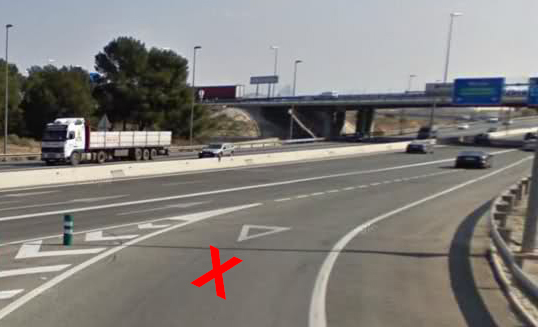
\includegraphics[width=\textwidth]{figures/3.1a.jpg}
    \caption{Opción 1}
    \label{fig:3.1a}
  \end{subfigure}
  \hfill
  \begin{subfigure}[b]{0.45\textwidth}
    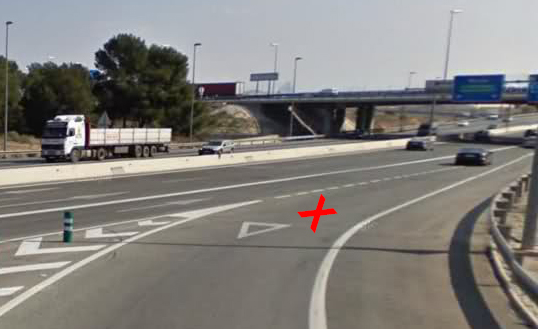
\includegraphics[width=\textwidth]{figures/3.1b.jpg}
    \caption{Opción 2}
    \label{fig:3.1b}
  \end{subfigure}
  \begin{subfigure}[b]{0.45\textwidth}
    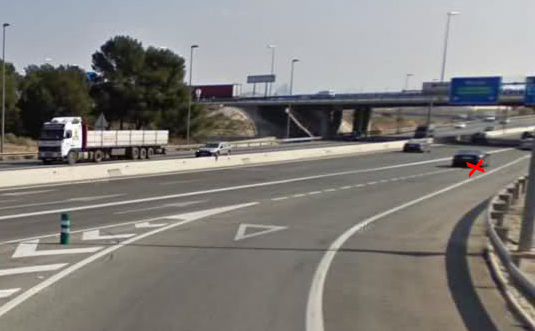
\includegraphics[width=\textwidth]{figures/3.1c.jpg}
    \caption{Opción 3}
    \label{fig:3.1c}
  \end{subfigure}
  \caption{Carril de aceleración, (a) antes de la señal, (b) después de la señal y (c) final del carril}
  \label{fig:3.1}
\end{figure}

Aproximadamente la mitad de los conductores, aun cuando se encontraron con un carril de incorporación corto y no viendo clara la salida, no pararían al principio del carril. Sin embargo, la mayor parte de los encuestados (más del 80\%) afirmaron que facilitarían la incorporación de los demás vehículos a la vía por la que circulan, siempre y cuando las condiciones se lo permitiesen. Por último, en una incorporación los conductores tendieron a fijarse en los vehículos que circulan dentro de la vía, en el vehículo que se encontrase delante y en la longitud del carril de aceleración. 

\subsubsection{3.1.1.3 Discusión}\label{3113}

Los resultados obtenidos de la encuesta sobre sensaciones y comportamientos en incorporaciones han permitido conocer en profundidad ciertos aspectos relacionados con el estrés durante la maniobra. Se observa que la experiencia en conducción y la edad guardan una relación lineal negativa con el estrés experimentado ante distintos escenarios de incorporación. Esto significa que existe una tendencia de los conductores más jóvenes y con menos experiencia a percibir más estrés en situaciones de incorporación a una vía. Hay que considerar que ambas variables están estrechamente ligadas, por lo que la variable experiencia es la más relevante en este contexto. 

En lo relativo a acciones, se observa que los conductores que informan de mayores niveles de estrés tienden a esperar hasta el final para frenar en las incorporaciones, son más arriesgados, comienzan prematuramente una incorporación si advierten que los vehículos que circulan detrás se van a incorporar primero y emplean el claxon en la autovía con mayor frecuencia que los no experimentan niveles altos de estrés. Por otro lado, se observa que los conductores suelen ser menos arriesgados en las incorporaciones cuando llevan a pasajeros en su vehículo. 

De manera general, se esperaban obtener mayores niveles de estrés frente a una incorporación, sin embargo, más del 70\% de los participantes informaron sentir poco o solo a veces estrés durante la maniobra. No obstante, estos niveles de estrés crecen si las condiciones de visibilidad son bajas o si llegan al final del carril sin velocidad suficiente. En esta última situación, la actitud de los conductores no es conservadora, ya que en caso de tener que detenerse, la mitad de los encuestados lo harían en el último tercio del carril, apoyando los resultados de \textcite{marczak}. A pesar de ello, también se observa una actitud colaborativa al manifestar en su mayoría que facilitarían la maniobra si las circunstancias lo permiten. 

Finalmente, se puede concluir que la incorporación es una maniobra muy intuitiva, la cual necesita práctica, y en cierta manera riesgo, ya que el conductor debe evaluar las intenciones de los demás vehículos utilizando solo la exploración visual como única fuente de información. Por todo ello es recomendable y beneficioso la integración de un sistema de ayuda a la incorporación con objeto de mejorar la seguridad y facilitar la realización de la maniobra.  

\subsection{Evaluación de variables atencionales en incorporaciones} \label{312}

El comportamiento visual está íntimamente ligado a la actividad cognitiva. Variables como la dirección de la mirada, las fijaciones y sacadas proporcionan información sobre la atención de la persona, pero también sobre la carga mental o el estrés, especialmente la dilatación pupilar. La complejidad de la situación tiene una relación directa con el diámetro de la pupila (\cite{wickens}; \cite{poock}), como es el ejemplo de la incorporación a una vía, donde se requiere procesar una alta cantidad de información. 

Para evaluar de manera objetiva la carga mental generada en el conductor por las situaciones de incorporación, se analiza el comportamiento visual de varios sujetos durante dicha maniobra en tráfico real, con el objetivo de diseñar una interfaz para un sistema de asistencia al conductor que facilite su incorporación al flujo vehicular. Mediante el estudio de las variables atencionales y el análisis correspondiente, se observará una influencia significativa de la carga cognitiva en la dirección de la mirada del conductor.

\subsubsection{3.1.2.1 Metodología}\label{3121}

Los sujetos que participaron en los ensayos de conducción fueron un total de 8, siendo 6 de ellos hombres y 2 mujeres. La edad y la experiencia de los participantes fue muy similar, obteniendo unos valores de 31.25 años (\emph{SD} = 4.23) para edad y 12.25 años (\emph{SD} = 4.30) para experiencia. La mayoría de los participantes manifestaron conducir de forma habitual un turismo como primer vehículo. En esta primera aproximación, el número de participantes se consideró suficiente para la obtención de resultados preliminares, los cuales fueron analizados mediante estudios estadísticos apropiados para el tamaño de la muestra. 

Los ensayos de conducción fueron realizados en un circuito en tráfico real en la zona sureste de Madrid, coincidiendo con las principales autovías M-30, M-40 y A-3 Carretera de Valencia con una duración media de 15 minutos cada uno. A lo largo de esta zona se encontraron entre 10 y 20 ocasiones donde observar situaciones de incorporación, tanto a izquierdas como a derechas gracias a los nudos entre carreteras, las cuales fueron analizadas independientemente del resto de trayecto realizado.  

Las dos condiciones principales a estudiar fueron por un lado los intervalos de incorporación y por otro, el resto del experimento, considerado como línea o tasa base. En esta última condición se instruyó a los participantes que condujeran de manera natural, obteniendo una referencia de cada uno de ellos para el análisis estadístico. Como criterio para definir el inicio de una incorporación se utilizó la primera mirada al retrovisor, ya que es en esta inspección visual donde el conductor extrajo la mayor parte de información del entorno para realizar la maniobra. El vehículo utilizado es un Peugeot 307 con cambio de marchas automático. Las respuestas oculares de los conductores han sido registradas mediante un sistema de seguimiento visual, extrayendo principalmente diámetros de pupila, fijaciones y posición en el espacio de la mirada.  
El sistema de seguimiento visual utilizado es el equipo Tobii Pro Glasses 2 (Figura \ref{fig:3.2}), cuyas ventajas frente a otros sistemas son la portabilidad y ligereza, dado que no necesita de elementos instalados permanentemente en el vehículo, la robustez ante diferencias lumínicas exteriores y la facilidad de calibración. 

\begin{figure}[h]
    \centering
    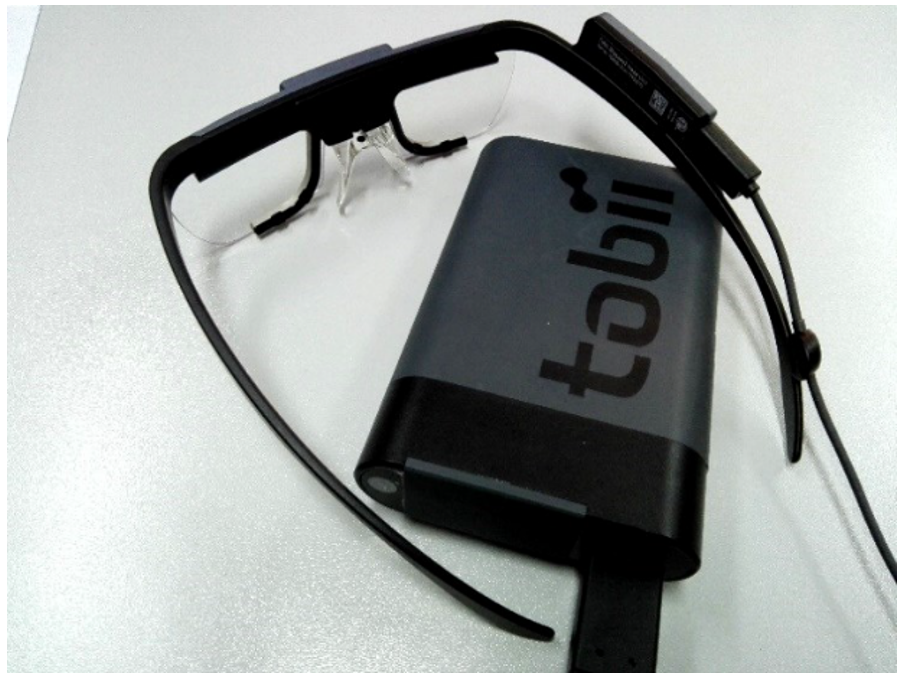
\includegraphics[width=9cm]{figures/3.2.png}
    \caption{ \label{fig:3.2} Tobii Pro Glasses 2}
\end{figure}

Las gafas están equipadas con 2 sensores infrarrojos y 4 cámaras, dos por cada ojo, permitiendo la adquisición de datos de la pupila y el comportamiento de la mirada. Además, una cámara situada en la parte delantera de las gafas adquiere información de la escena y permite ubicar la mirada del conductor en la carretera. La técnica para la detección de la mirada es el método pupila oscura, iluminando la mirada de manera no coaxial y haciendo que la pupila aparezca sombreada. El equipo se conecta mediante Ethernet al ordenador de control, capturando las siguientes variables (Tabla \ref{tab:3.2}).

Además de estas variables, se han realizado análisis de las áreas de interés durante la maniobra de incorporación y los mapas de calor de las miradas, gracias al software de la misma compañía Tobii Pro Lab.
Se han llevado a cabo análisis estadísticos no paramétricos debido al limitado tamaño de muestra empleada. Para ello se realizó la prueba de los rasgos con signo de Wilcoxon para muestras pareadas con el software SPSS v26, con objeto de comprobar si existen diferencias significativas entre ambas muestras. 

\newpage
\begin{table}[htb]
\centering
\begin{tabular}{@{}rll@{}}
\textbf{Variables}                                                                                       & \textbf{Descripción  }                                                                                                   & \textbf{Unidades}                                                                                              \\ \midrule
\begin{tabular}[c]{@{}r@{}}Dirección de la Mirada\\ (Izquierda y derecha)\end{tabular} & Dirección de la mirada en ambos ojos                                                                            & Milímetros                                                                                            \\ \midrule
Posición de la mirada 2D                                                               & \begin{tabular}[c]{@{}l@{}}Posición de la mirada dentro de los \\   límites del marco de grabación\end{tabular} & \begin{tabular}[c]{@{}l@{}}Arriba-izquierda {[}0, 0{]}\\ Abajo- derecha {[}1, 1{]}\end{tabular} \\ \midrule
Posición de la mirada 3D                                                              & La posición de la pupila en un espacio 3D                                                                       & Milímetros                                                                                            \\ \midrule
\begin{tabular}[c]{@{}r@{}}Diámetro de la pupila\\ (Izquierda y derecha)\end{tabular}  & Diámetro de la pupila en ambos ojos                                                                             & Milímetros                                                                                            \\ \midrule
\begin{tabular}[c]{@{}r@{}}Centro de la pupila  \\  (Izquierda y derecha)\end{tabular} & Centro de la pupila en ambos ojos                                                                               & Milímetros                                                                                            \\ \midrule
Giróscopo                                                                             & Velocidad angular en cada uno de los tres   ejes                                                                & °/s                                                                                                   \\ \midrule
Acelerómetro                                                                           & \begin{tabular}[c]{@{}l@{}}Aceleración de cada una de las tres \\   direcciones espaciales\end{tabular}         & m/s²                                                                                                  \\ \midrule
Vídeo                                                                                  & Grabación del ensayo                                                                                            & \begin{tabular}[c]{@{}l@{}}1920 x 1080 píxeles a \\ 25 fps\end{tabular}                               \\ \midrule
Frecuencia de muestreo                                                                 &                                                                                                                 & 50 Hz                                                                                                 \\ \bottomrule
\end{tabular}
\caption{Variables del sistema de seguimiento visual Tobii Pro Glasses 2}
\label{tab:3.2}
\end{table}

\subsubsection{3.1.2.2 Resultados}\label{3122}

\textbf{\emph{Diámetro de las pupilas}}

La mayoría de los diámetros de las pupilas de los conductores mostraron sensibilidad en las situaciones de incorporación a vías principales, aumentando su valor respecto a la línea base obtenida en conducción normal, marcado con color azul en la tabla \ref{tab:3.3}. 

\begin{table}[htb]
\centering
\begin{tabular}{@{}cccccccccll@{}}
                                            & \multicolumn{10}{c}{\textbf{Diámetro de la pupila (mm)}}                                                                                                                                                                                                                                                                                  \\ \cmidrule(l){2-11} 
                                            & \multicolumn{4}{c|}{Incorporaciones}                                                                                                                                & \multicolumn{6}{c}{Tasa   base}                                                                                                                                     \\ \cmidrule(l){2-11} 
                                            & \multicolumn{2}{c|}{\textit{Ojo Izq.}}                                           & \multicolumn{2}{c|}{\textit{Ojo   Dcho.}}                                        & \multicolumn{2}{c}{\textit{Ojo   Izq.}}                                          & \multicolumn{4}{c}{\textit{Ojo   Dcho.}}                                         \\ \cmidrule(l){2-11} 
\multirow{-4}{*}{\textbf{Sujetos}} & \textit{M}                   & \multicolumn{1}{c|}{\textit{SD}}                  & \textit{M}                   & \multicolumn{1}{c|}{\textit{SD}}                  & \textit{M}                   & \multicolumn{1}{c|}{\textit{SD}}                  & \textit{M}                    & \multicolumn{3}{c}{\textit{SD}}                  \\ \cmidrule(l){2-11} 
{A}                                  & \cellcolor[HTML]{BDD6EE}2.71 & \multicolumn{1}{c|}{\cellcolor[HTML]{BDD6EE}0.30} & \cellcolor[HTML]{BDD6EE}2.70 & \multicolumn{1}{c|}{\cellcolor[HTML]{BDD6EE}0.28} & 2.63                         & \multicolumn{1}{c|}{0.26}                         & 2.57                          & \multicolumn{3}{c}{0.27}                         \\ \midrule
{B}                                  & 1.87                         & \multicolumn{1}{c|}{0.18}                         & 1.83                         & \multicolumn{1}{c|}{0.15}                         & \cellcolor[HTML]{BDD6EE}1.89 & \multicolumn{1}{c|}{\cellcolor[HTML]{BDD6EE}0.17} & \cellcolor[HTML]{BDD6EE}1.88  & \multicolumn{3}{c}{\cellcolor[HTML]{BDD6EE}0.16} \\ \midrule
{C}                                  & \cellcolor[HTML]{BDD6EE}2.42 & \multicolumn{1}{c|}{\cellcolor[HTML]{BDD6EE}0.22} & \cellcolor[HTML]{BDD6EE}2.34 & \multicolumn{1}{c|}{\cellcolor[HTML]{BDD6EE}0.24} & 2.32                         & \multicolumn{1}{c|}{0.16}                         & 2.26                          & \multicolumn{3}{c}{0.18}                         \\ \midrule
{D}                                  & \cellcolor[HTML]{BDD6EE}2.49 & \multicolumn{1}{c|}{\cellcolor[HTML]{BDD6EE}0.23} & \cellcolor[HTML]{BDD6EE}2.56 & \multicolumn{1}{c|}{\cellcolor[HTML]{BDD6EE}0.25} & 2.46                         & \multicolumn{1}{c|}{0.27}                         & 2.45                          & \multicolumn{3}{c}{0.30}                         \\ \midrule
{E}                                  & \cellcolor[HTML]{BDD6EE}3.49 & \multicolumn{1}{c|}{\cellcolor[HTML]{BDD6EE}1.36} & \cellcolor[HTML]{BDD6EE}3.47 & \multicolumn{1}{c|}{\cellcolor[HTML]{BDD6EE}1.30} & 2.41                         & \multicolumn{1}{c|}{1.23}                         & 2.43                          & \multicolumn{3}{c}{1.22}                         \\ \midrule
{F}                                  & \cellcolor[HTML]{BDD6EE}2.48 & \multicolumn{1}{c|}{\cellcolor[HTML]{BDD6EE}0.31} & \cellcolor[HTML]{BDD6EE}2.46 & \multicolumn{1}{c|}{\cellcolor[HTML]{BDD6EE}0.29} & 2.29                         & \multicolumn{1}{c|}{0.36}                         & 2.24                          & \multicolumn{3}{c}{0.19}                         \\ \midrule
G                                           & \cellcolor[HTML]{BDD6EE}2.10 & \multicolumn{1}{c|}{\cellcolor[HTML]{BDD6EE}0.20} & \cellcolor[HTML]{BDD6EE}2.09 & \multicolumn{1}{c|}{\cellcolor[HTML]{BDD6EE}0.22} & 1.96                         & \multicolumn{1}{c|}{0.17}                         & 1.96                          & \multicolumn{3}{c}{0.17}                         \\ \midrule
H                                           & \cellcolor[HTML]{BDD6EE}1.87 & \multicolumn{1}{c|}{\cellcolor[HTML]{BDD6EE}0.20} & \cellcolor[HTML]{BDD6EE}1.85 & \multicolumn{1}{c|}{\cellcolor[HTML]{BDD6EE}0.15} & 1.83                         & \multicolumn{1}{c|}{0.16}                         & 1.77                          & \multicolumn{3}{c}{0.16}                        
\end{tabular}
\caption{Media y desviación típica del diámetro de la pupila}
\label{tab:3.3}
\end{table}

Este incremento puede verse en términos porcentuales en la figura \ref{fig:3.3}, donde la mayoría de los participantes tuvieron un aumento en la media pupilar durante la incorporación respecto a la tasa base. Excluyendo los valores atípicos se puede resumir que el diámetro pupilar aumentó aproximadamente un 5.3\% para el ojo derecho y un 4.13\% para el ojo izquierdo durante la maniobra de incorporación.

\begin{figure}[h]
    \centering
    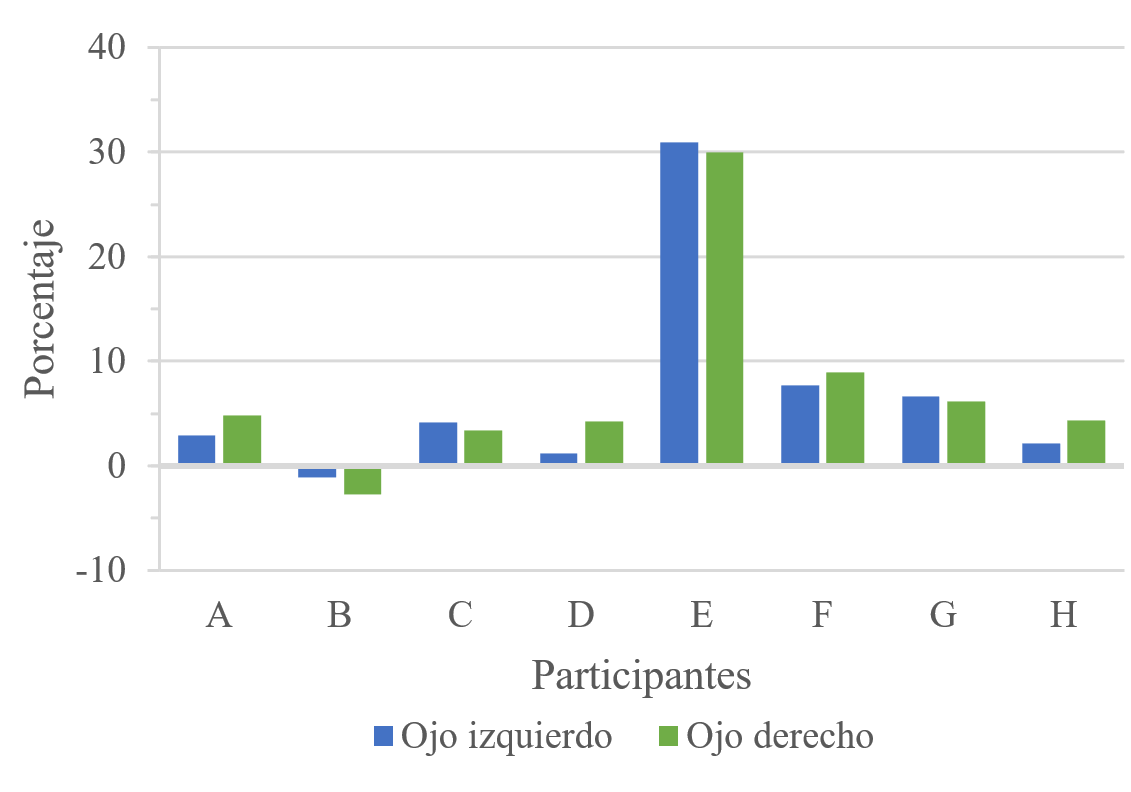
\includegraphics[width=12cm]
    {figures/3.3.png}
    \caption{ \label{fig:3.3} Porcentaje de aumento de la media pupilar en incorporaciones}
\end{figure}

A nivel estadístico se realizó una prueba de Wilcoxon, obteniendo diferencias significativas tanto para la pupila izquierda (\emph{Z} = 2.1, \emph{p} = 0.036) como en la pupila derecha (\emph{Z} = 2.38, \emph{p} = 0.016) entre las situaciones de incorporación y tasa base. 

\textbf{\emph{Fijaciones}}

Los datos obtenidos de las fijaciones permitieron realizar diferentes análisis donde observar el efecto de una incorporación en el comportamiento visual los conductores. Se han examinado los momentos de incorporación frente al resto del ensayo, y posteriormente, la influencia de los espejos retrovisores durante la maniobra.
En la duración de las fijaciones en incorporaciones frente a tasa base no se encontraron resultados significativos, ni una tendencia remarcable como se puede observar en la tabla \ref{tab:3.4}. Estos resultados son debido a la variabilidad que existe entre las diferentes áreas observadas durante una incorporación, reflejada además en los valores de desviación típica.

\newpage
\begin{table}[h]
\centering
\begin{tabular}{@{}cccccccccll@{}}
\multirow{5}{*}{\textbf{Sujetos}} & \multicolumn{10}{c}{\textbf{Duración de las fijaciones (ms)}}                       \\ \cmidrule(l){2-11} 
                                           & \multicolumn{2}{c|}{Incorporaciones}                      & \multicolumn{2}{c}{Tasa   base}                                  \\ \cmidrule(l){2-11} 
                                           & \textit{M} & \multicolumn{1}{c|}{\textit{SD}} & \textit{M} & \multicolumn{1}{c}{\textit{SD}} \\ \cmidrule(l){2-11} 
{A}                                 & 551.83     & \multicolumn{1}{c|}{783.51}      & 462.36     & \multicolumn{1}{c}{517.23}      \\ \midrule
{B}                                 & 382.17     & \multicolumn{1}{c|}{355.14}      & 342.68     & \multicolumn{1}{c}{548.21}      \\ \midrule
{C}                                 & 551.83     & \multicolumn{1}{c|}{783.51}      & 398.82     & \multicolumn{1}{c}{374.64}      \\ \midrule
{D}                                 & 210.30     & \multicolumn{1}{c|}{188.11}      & 341.80     & \multicolumn{1}{c}{455.22}     \\ \midrule
{E}                                 & 171.86     & \multicolumn{1}{c|}{131.30}      & 257.90     & \multicolumn{1}{c}{221.65}       \\ \midrule
{F}                                 & 1850.88    & \multicolumn{1}{c|}{1894.98}     & 787.44     & \multicolumn{1}{c}{1059.73}       \\ \midrule
G                                   & 294.61     & \multicolumn{1}{c|}{262.47}      & 299.20     & \multicolumn{1}{c}{252.75}     \\ \midrule
H                                   & 282.59     & \multicolumn{1}{c|}{374.36}      & 291.56     & \multicolumn{1}{c}{244.35}       \\ \midrule
\end{tabular}
\caption{Media y desviación típica de la duración de las fijaciones}
\label{tab:3.4}
\end{table}

El siguiente análisis se particularizó al área de los espejos retrovisores, evaluando la duración y número de fijaciones a los mismos respecto a las totales realizadas durante la maniobra de incorporación en términos porcentuales. Los resultados obtenidos se resumen en la tabla \ref{tab:3.5}, diferenciando entre incorporación a izquierdas y derechas.

\begin{table}[htbp]
\centering
\begin{tabular}{@{}ccc|cc@{}}
\multirow{2}{*}{\textbf{Sujetos}} & \multicolumn{2}{c|}{\textbf{\begin{tabular}[c]{@{}c@{}}\% Duración fijaciones en espejos \\ retrovisores respecto al total\end{tabular}}} & \multicolumn{2}{c}{\textbf{\begin{tabular}[c]{@{}c@{}}\% Número fijaciones en espejos \\ retrovisores respecto al total\end{tabular}}} \\ \cmidrule(l){2-5} 
                                  & \textit{Espejo   Izq.}                                              & \textit{Espejo   Dcho.}                                             & \textit{Espejo   Izq.}                                            & \textit{Espejo   Dcho.}                                            \\ \cmidrule(l){2-5} 
{A}                        & 44.46                                                               & 37.44                                                               & 45.7                                                              & 40.44                                                              \\ \midrule
{B}                        & 21.39                                                               & 21.76                                                               & 22.48                                                             & 19.86                                                              \\ \midrule
{C}                        & 36.33                                                               & 58.91                                                               & 53.37                                                             & 50.87                                                              \\ \midrule
{D}                        & 13.81                                                               & 38.02                                                               & 16.8                                                              & 37.34                                                              \\ \midrule
{E}                        & 7.56                                                                & 17.31                                                               & 18.48                                                             & 36.67                                                              \\ \midrule
{F}                        & 0                                                                   & 46.76                                                               & 0                                                                 & 33.82                                                              \\ \midrule
{G}                        & 39.16                                                               & 48.62                                                               & 16.8                                                              & 47.82                                                              \\ \midrule
{H}                        & 31.36                                                               & 42.99                                                               & 33.75                                                             & 37.66                                                              \\ \midrule
{Media total}              & 24.26                                                               & 38.98                                                               & 25.92                                                             & 38.06                                                              \\ \bottomrule
\end{tabular}
\caption{Porcentaje de duración de las fijaciones en los espejos retrovisores}
\label{tab:3.5}
\end{table}

De manera general se aprecia que las miradas a los espejos constituyen aproximadamente un 30\% de las totales respecto al resto de elementos observados en una incorporación, como pueden ser el panel de mandos, el propio carril, los carriles adyacentes o el espejo interior.  Diferenciando entre incorporación a izquierdas o a derechas, se puede observar que, en su mayoría, los valores de duración de las fijaciones y número de fijaciones son más grandes hacia derechas que hacía izquierdas en la mayoría de los participantes.

\newpage
\textbf{\emph{Mapas de calor y áreas de interés}}

En un análisis más focalizado en la maniobra de incorporación se evaluó la mirada del conductor hacia las principales áreas de interés de su entorno. De cada maniobra, se generó el mapa de calor correspondiente a la ubicación de las miradas en el habitáculo, siendo más intensas las zonas con más densidad de miradas. En las siguientes imágenes se pueden observar dos ejemplos de mapas de calor en situaciones de incorporación hacia el carril izquierdo (Figura \ref{fig:3.4a}) y hacia el carril derecho (Figura \ref{fig:3.4b}).

\begin{figure}[h]
  \centering
  \begin{subfigure}[b]{0.45\textwidth}
    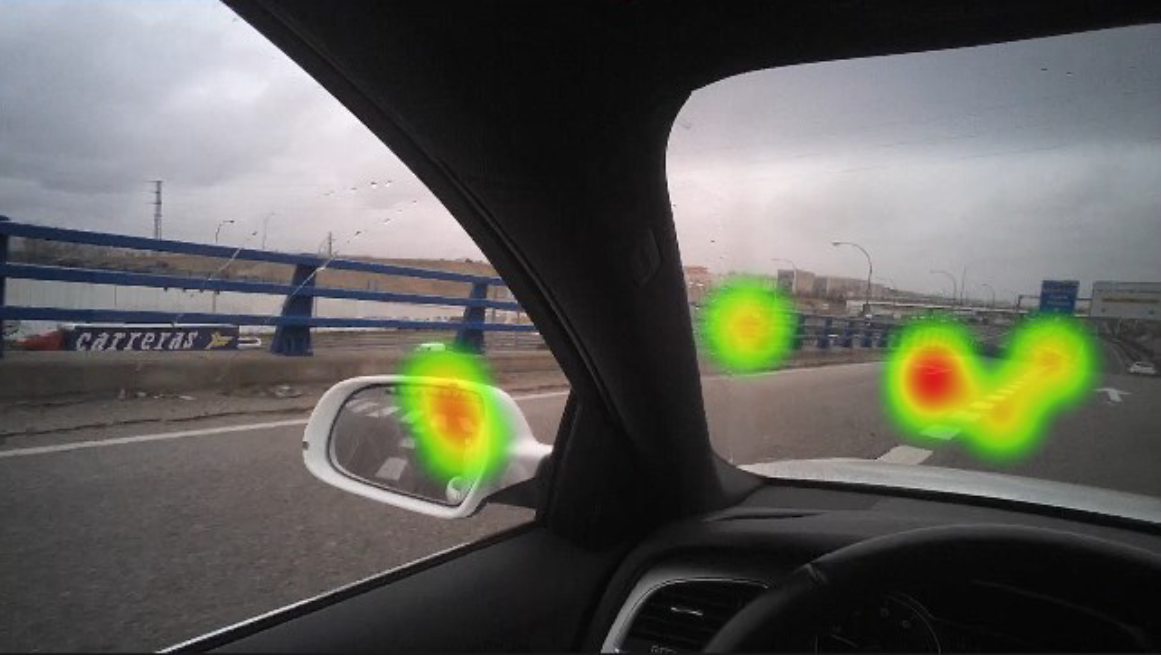
\includegraphics[width=\textwidth]{figures/3.4a.png}
     \caption{}\label{fig:3.4a}
  \end{subfigure}
  \hfill
  \begin{subfigure}[b]{0.45\textwidth}
    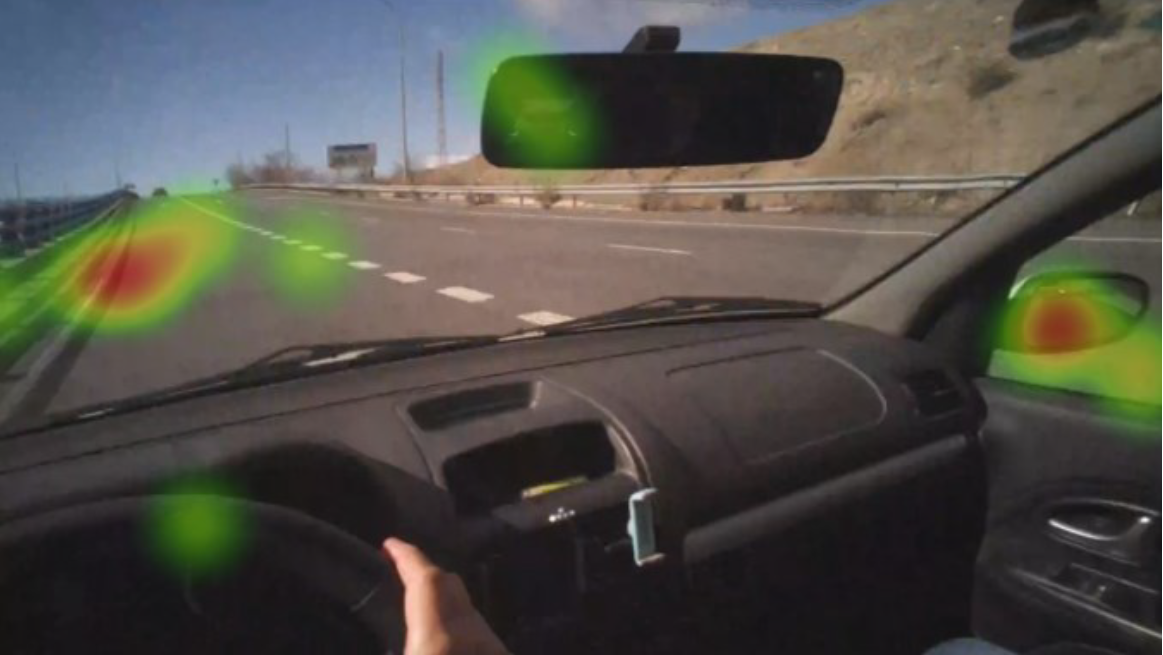
\includegraphics[width=\textwidth]{figures/3.4b.png}
     \caption{}\label{fig:3.4b}
  \end{subfigure}
  \caption{Mapas de calor de la actividad visual: (a) en incorporación hacia el carril izquierdo, (b) en incorporación hacia el carril derecho}
  \label{fig:3.4}
\end{figure}

En la mayoría de los mapas analizados de todos los participantes, es destacable un punto caliente común a ambos espejos retrovisores en la zona superior-interior del cristal, como se aprecia en las anteriores imágenes. 
En el análisis de las áreas de interés, se ha segmentado la imagen en las siguientes zonas: coche/salpicadero, señal, carril central, carril derecho, carril izquierdo, espejo retrovisor derecho, espejo retrovisor izquierdo y espejo interior (Figuras \ref{fig:3.5a} y \ref{fig:3.5b}). Cabe destacar que, debido a la escasez de datos, las medidas tomadas de las áreas señales, carril derecho, espejo retrovisor derecho y espejo interior han sido excluidas del análisis. 

\begin{figure}[h]
  \centering
  \begin{subfigure}[b]{0.45\textwidth}
    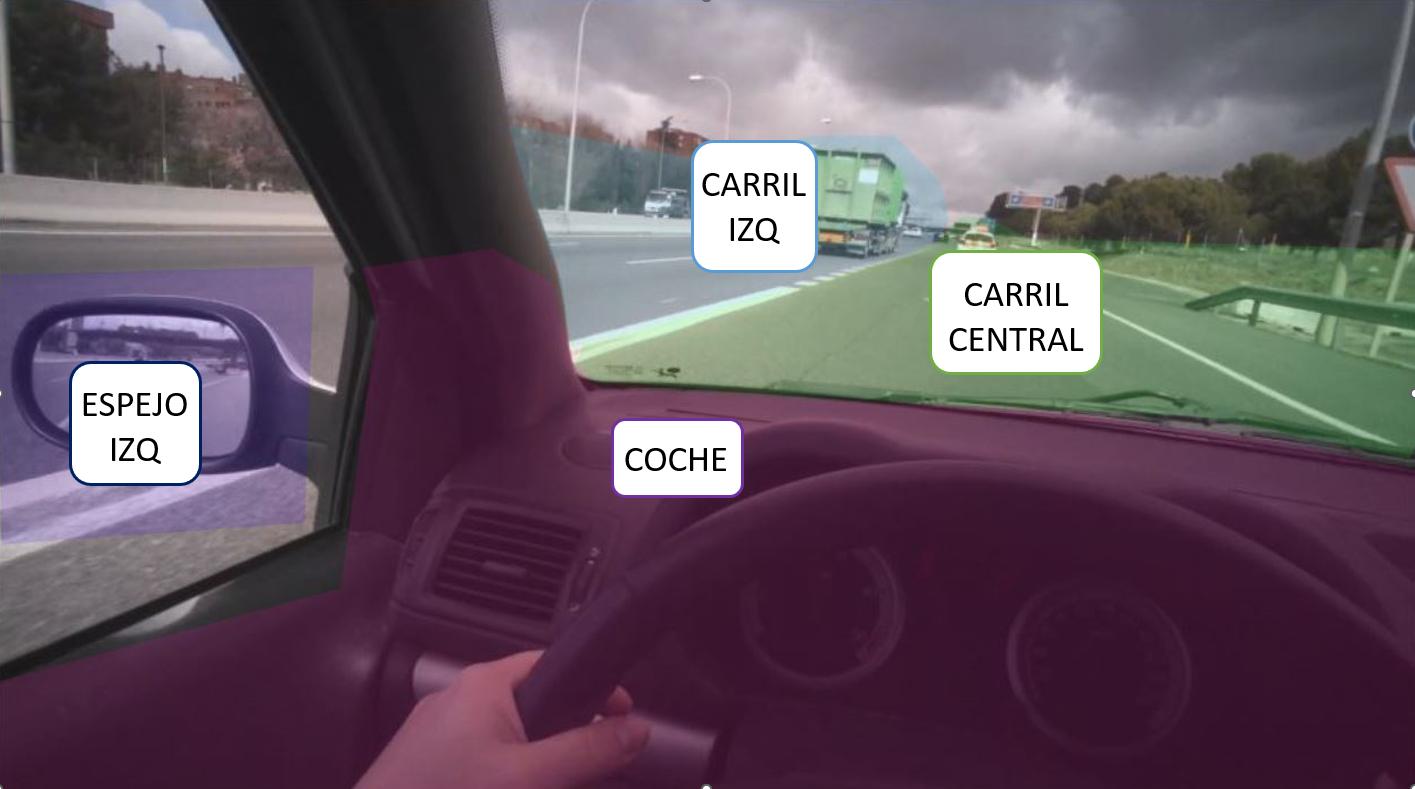
\includegraphics[width=\textwidth]{figures/3.5a.png}
    \caption{}\label{fig:3.5a}
  \end{subfigure}
  \hfill
  \begin{subfigure}[b]{0.45\textwidth}
    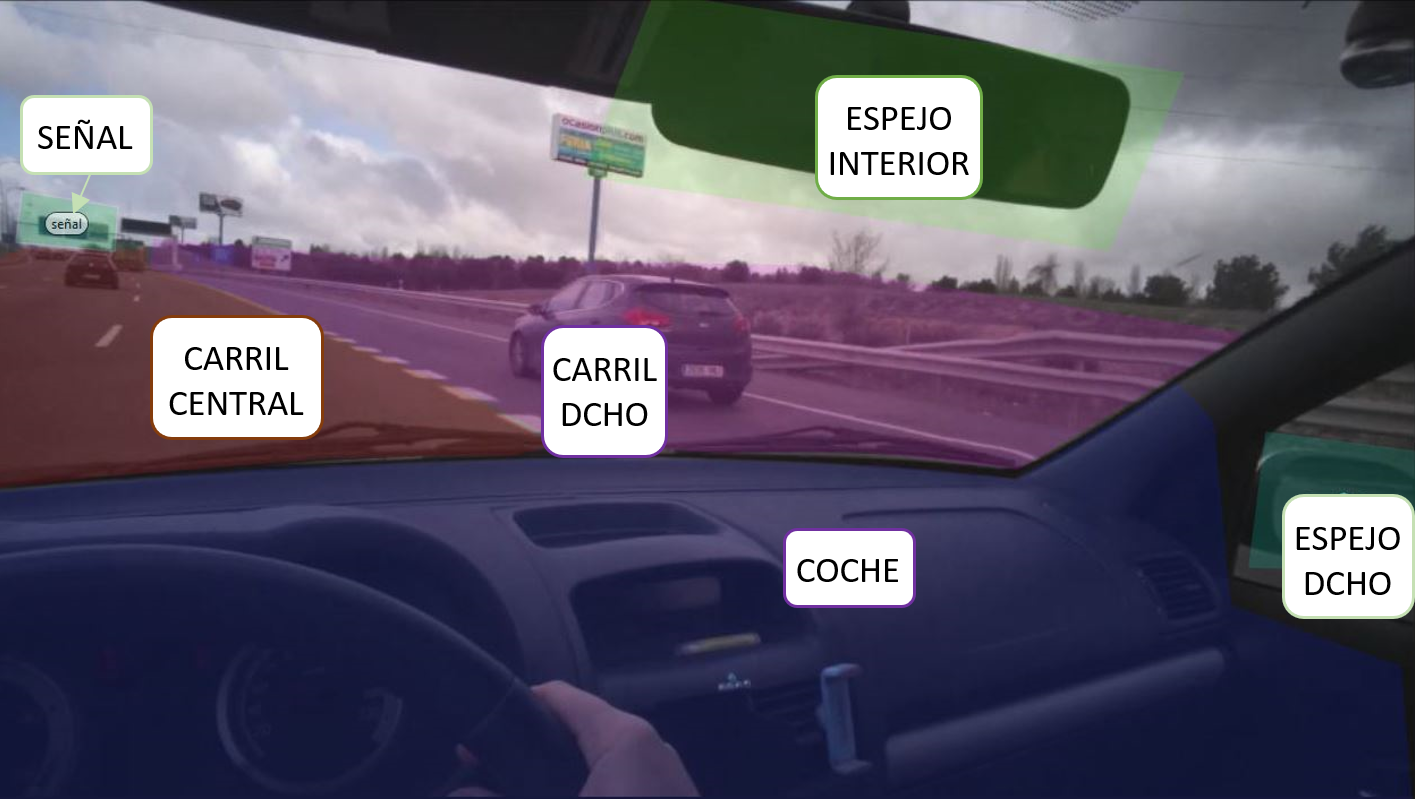
\includegraphics[width=\textwidth]{figures/3.5b.png}
    \caption{}\label{fig:3.5b}
  \end{subfigure}
  \caption{Segmentación de áreas de interés: (a) en incorporación hacia el carril izquierdo, (b) en incorporación hacia el carril derecho}
  \label{fig:3.5}
\end{figure}

Las variables a estudiar fueron la duración total de las fijaciones, el número total de fijaciones y la duración de la primera fijación en el área. Una prueba no paramétrica de Wilcoxon para hallar diferencias significativas entre el periodo de incorporación y la tasa base de cada zona, se realizó sobre cada uno de estos tres parámetros, obteniendo resultados desde tres puntos de vista diferentes. Dado que no todas las incorporaciones duraron lo mismo, se han reformulado los datos tomados expresándolos en relación con intervalo de tiempo que duró el evento. Posteriormente, se han mediado los valores correspondientes a las incorporaciones y a la tasa base de cada sujeto, obteniendo así una pareja de valores por participante. En la tabla \ref{tab:3.6} se muestran los resultados de la prueba no paramétrica, donde se observan las diferencias significativas en las medianas de los tres parámetros propuestos para cada área de interés, comparando entre situación de tasa base e incorporación.

\begin{table}[ht]
\centering
\resizebox{\textwidth}{!}{%
\begin{tabular}{cccc}
\textbf{Áreas de interés} & \textbf{\begin{tabular}[c]{@{}c@{}}Duración de\\ fijaciones / segundo\end{tabular}} & \textbf{\begin{tabular}[c]{@{}c@{}}Número de \\ fijaciones / segundo\end{tabular}} & \textbf{\begin{tabular}[c]{@{}c@{}}Duración de la primera \\ fijación / segundo\end{tabular}} \\ \hline
{Carril   central}          & \begin{tabular}[c]{@{}c@{}}Si   (línea base alta, \\ \emph{p} = 0.018)\end{tabular}      & No                                                                                 & \begin{tabular}[c]{@{}c@{}}Si   (línea base baja, \\ \emph{p} = 0.018)\end{tabular}                  \\ \hline
{Carril   izquierdo}        & No                                                                                & No                                                                                 & \begin{tabular}[c]{@{}c@{}}Si   (línea base baja, \\ \emph{p} = 0.018)\end{tabular}                  \\ \hline
{Espejo   izquierdo}        & \begin{tabular}[c]{@{}c@{}}Si   (línea base baja, \\ \emph{p} = 0.018)\end{tabular}      & \begin{tabular}[c]{@{}c@{}}Si   (línea base baja,   \\  \emph{p}   = 0.018)\end{tabular}  & \begin{tabular}[c]{@{}c@{}}Si   (línea base baja, \\ \emph{p} = 0.028)\end{tabular}                  \\ \hline
{Coche/Salpicadero}         & No                                                                                & No                                                                                 & No                                                                                            \\ \hline
\end{tabular}%
}
\caption{Diferencias significativas entre tasa base e incorporación en las áreas de interés}
\label{tab:3.6}
\end{table}
 
Los resultados más destacables se observan en la duración de la primera fijación, el cual fue superior en escenarios de incorporación para casi todas las áreas de interés, debido al análisis de la situación previo a la realización de la maniobra. En el espejo izquierdo todas las variables de seguimiento visual analizadas fueron superiores durante la incorporación, reforzando los resultados previamente obtenidos en las fijaciones y los mapas de calor. Contrariamente, el carril central se obtuvo una duración de las fijaciones mayor durante la tasa base, dado que durante una conducción crucero el conductor fija toda su atención en esta área. 

Por último, se analizaron de nuevo las diferencias significativas entre áreas durante una incorporación, en los parámetros de duración total y número de fijaciones por segundo. El parámetro de duración de la primera fijación se excluyó de este análisis debido a la escasez de datos para poder realizar la prueba estadística. Los resultados obtenidos se representan en la tabla \ref{tab:3.7}, relacionando las diferentes áreas entre sí.

\begin{table}[hb]
\centering
\resizebox{\textwidth}{!}{%
\begin{tabular}{ccc}
\textbf{Áreas de interés}                                                                & \textbf{Duración fijaciones / segundo}                                                               & \textbf{Número de fijaciones / segundo}                                                            \\ \hline
{Carril central – Carril   izq.}                                                  & \begin{tabular}[c]{@{}c@{}}Si (Carril central \textgreater   Carril izq., \\ \emph{p} = 0.028)\end{tabular} & No                                                                                                 \\ \hline
{Carril central – Espejo   izq.}                                                  & No                                                                                                   & No                                                                                                 \\ \hline
{\begin{tabular}[c]{@{}c@{}}Carril central –   \\ Coche/Salpicadero\end{tabular}} & \begin{tabular}[c]{@{}c@{}}Si (Carril central \textgreater   Coche,\\ \emph{p}   = 0.028)\end{tabular}      & \begin{tabular}[c]{@{}c@{}}Si (Carril central \textgreater   Coche,   \\ \emph{p}   = 0.028)\end{tabular} \\ \hline
{Carril izq. – Espejo   izq.}                                                     & No                                                                                                   & \begin{tabular}[c]{@{}c@{}}Si (Carril izq. \textless   Espejo izq., \\ \emph{p}   = 0.028)\end{tabular}   \\ \hline
{\begin{tabular}[c]{@{}c@{}}Carril izq. –   \\ Coche/Salpicadero\end{tabular}}    & No                                                                                                   & \begin{tabular}[c]{@{}c@{}}Si (Carril izq. \textgreater   Coche, \\ \emph{p}   = 0.043)\end{tabular}      \\ \hline
{\begin{tabular}[c]{@{}c@{}}Espejo izq. – \\ Coche/Salpicadero\end{tabular}}      & \begin{tabular}[c]{@{}c@{}}Si (Espejo izq. \textgreater Coche, \\ \emph{p}   = 0.028)\end{tabular}          & \begin{tabular}[c]{@{}c@{}}Si (Espejo izq. \textgreater Coche, \\ \emph{p}   = 0.018)\end{tabular}        \\ \hline
\end{tabular}%
}
\caption{Diferencias significativas en duración y número de fijaciones por segundo entre áreas de interés}
\label{tab:3.7}
\end{table}

\newpage
Se observa que el área con menos diferencias entre la situación de incorporación y la tasa base fue el área coche o salpicadero, no apareciendo como la variable más alta en ninguna de las comparaciones de las dos tablas. No obstante, en el área espejo izquierdo y carril central se obtuvieron valores más altos durante la incorporación en ambas tablas, duración y número de fijaciones, siendo estas zonas muy observadas por conductor en la realización de la maniobra. 

\subsubsection{3.1.2.3	Discusión}\label{3123}

En este estudio se ha analizado la influencia de las variables atencionales de un conductor durante la maniobra de incorporación en tráfico real. A través de un sistema de seguimiento visual, se han obtenido diferencias significativas en ambas dilataciones pupilares, aumentando su valor alrededor de un 5\% durante la incorporación frente a la tasa base. 

Sin embargo, este resultado no se ve replicado en la duración de las fijaciones representada en la tabla  \ref{tab:3.5}, las cuales sí revelaron que aproximadamente un 30\% de las mismas se hacían a los espejos retrovisores en comparación con el resto de elementos que son observados durante una incorporación, como son el panel de mandos, el carril central, carriles adyacentes o el espejo interior. Este valor pone de manifiesto la importancia en el diseño y el uso de los espejos retrovisores, dado que gran parte del tiempo es dedicado a la exploración del entorno a través de ellos para poder realizar una maniobra lo más segura posible.

En relación con las fijaciones a los dos espejos retrovisores (Tabla \ref{tab:3.5}) se observó que, tanto la duración de las fijaciones como el número de las mismas, fueron más frecuentes a derechas que a izquierdas, pudiendo deberse a diferentes razones. Por un lado, en las incorporaciones a izquierdas se observó un mayor uso del espejo interior como complemento al espejo izquierdo, dando como resultado menores fijaciones al espejo izquierdo en comparación con el derecho. Por otro, este fenómeno también podría estar relacionado con la inseguridad y falta de hábito por parte de los conductores de realizar una incorporación a derechas, ya que la más común es a izquierdas y tiene una estructura muy similar a la maniobra de cambio de carril. Además, las incorporaciones a derechas requieren un giro de la cabeza más amplio, siendo este movimiento poco natural para el conductor. Un mayor tiempo en las fijaciones puede ser interpretado como una exploración en profundidad del entorno debido a su complejidad. El mismo efecto puede ser observado con un mayor número de fijaciones aun siendo su duración menor, ya que un número alto de fijaciones señala la necesidad de volver a explorar la situación.

En los mapas de calor se observó un punto caliente interesante en la esquina superior-interior del espejo, común a ambos retrovisores. Este resultado revela la gestión atencional de los conductores ante la demanda cognitiva de la situación de incorporación. Se puede concluir que la elección de esta zona es debido a que no está demasiado alejada del centro de la calzada, pero a su vez aporta suficiente información del carril lateral gracias a la visión periférica. Esta zona se considera interesante para la ubicación de futuras interfaces de ayuda a la conducción.

En el análisis de las áreas de interés se encontraron limitaciones del sistema, debiendo postprocesar parte de los datos manualmente. En los ensayos se advirtió que algunos conductores realizaron movimientos corporales y giros de cabeza bastante bruscos y frecuentes, especialmente cuando se miraba al espejo retrovisor derecho y en las incorporaciones a una vía. A pesar de que el sistema de adquisición dispone de un giróscopo y un acelerómetro para determinar el movimiento de la cabeza del conductor, y por tanto la dirección de su mirada, la propia deriva característica de los sensores junto a la longitud de los ensayos de conducción supuso la aparición de un error acumulativo. En consecuencia y para asegurar una buena calidad de los resultados, se suprimió dicha fuente de datos y se palió mediante una codificación manual de las áreas y los giros de la cabeza. En el siguiente capítulo se presenta una solución de bajo costo que resuelve de forma automática dichos inconvenientes. 

Los resultados mostraron la importancia de la primera fijación en todas las áreas de interés, evidenciando resultados estadísticamente significativos entre la tasa base y la incorporación. Como se presuponía, las primeras fijaciones durante una incorporación son más largas que en el periodo de tasa base, debido a la gran cantidad de información del entorno necesaria para la toma de decisiones. Por otro lado, también se advierte una mayor duración y número de fijaciones en el espejo izquierdo durante la incorporación, siendo este resultado coherente con los obtenidos en los mapas de calor, porcentaje de fijaciones en los espejos y diámetro de la pupila. 

Con respecto al carril central, la duración de las fijaciones es mayor en la tasa base que en la incorporación, a diferencia de otras zonas. Este resultado tiene mucho sentido, ya que en conducción normal el conductor centra la mayor parte de su atención en el obstáculo que se encuentra frente a su vehículo. 

En la comparación entre áreas de interés durante la maniobra de incorporación se observó que la zona del coche o salpicadero fue la que menos fijaciones en duración y número obtuvo, a diferencia del espejo izquierdo y el carril central. Este resultado se muestra en la tabla \ref{tab:3.7} donde no aparece en ningún caso como la variable más alta. La información que proporciona esta zona no es consideraba relevante en una situación de incorporación, todo lo contrario que la que se adquiere del espejo izquierdo, donde sí hay diferencias significativas tanto en duración como en número de fijaciones respecto al coche/salpicadero. De la misma forma, también se aprecian diferencias entre el carril central y el coche/salpicadero, viéndose reforzada la afirmación anterior.

En el siguiente estudio se plantea una interfaz de ayuda a la conducción para situaciones de incorporación, con la expectativa de que el conductor aumente las miradas al vehículo delantero y así pueda prestar atención conjuntamente al vehículo y a la carretera. 

\subsection{Sistema de asistencia en incorporaciones y diseño de HMI}\label{313}

Las situaciones de incorporación en autovías son situaciones complejas para los conductores, los cuales deben manejar mucha información en un periodo corto de tiempo tal y como se ha visto en el apartado anterior. El sistema propuesto se basa en un estudio previo donde se desarrolló un dispositivo de adaptación inteligente de la velocidad (\cite{jimenez12}). Dicho sistema informaba al conductor sobre la velocidad que debía adquirir al llegar a un tramo de carretera y le sugería, en términos cualitativos, cuánto aumentar o disminuir su velocidad al acercarse a ese tramo. En este caso, el sistema de asistencia a la incorporación proporciona al conductor información similar sobre cómo adaptar su velocidad para incorporarse a la carretera principal. 

El funcionamiento del sistema de ayuda a las incorporaciones puede resumirse en la figura \ref{fig:3.6}, donde el vehículo 1 calcula el hueco disponible entre los vehículos 2 y 3 para realizar la maniobra, respetando siempre un margen de seguridad, \emph{T}. Si finalmente no fuera posible, recomendaría al conductor esperar para incorporarse después del vehículo 3. 

\begin{figure}[h]
    \centering
    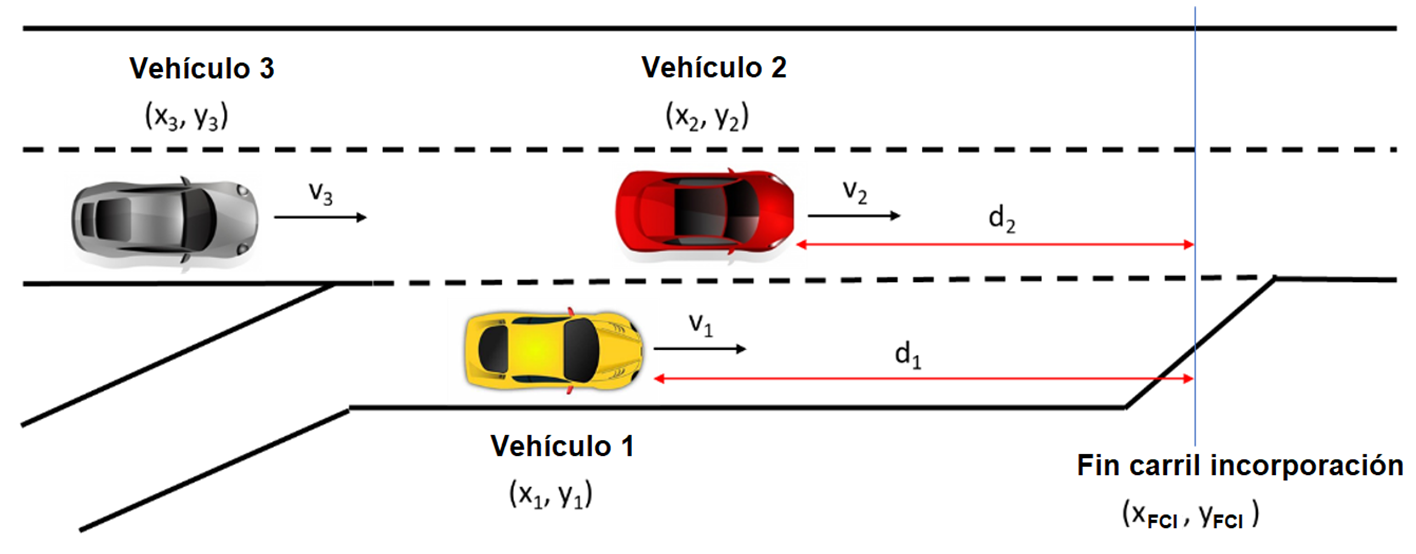
\includegraphics[width=12.5cm]
    {figures/3.6.png}
    \caption{ \label{fig:3.6} Vehículo en el carril de incorporación (vehículo 1), en la carretera principal (vehículos 2 y 3) y variables que intervienen en el algoritmo}
\end{figure}

Por otro lado, las interfaces hombre-máquina (\gls{hmi}) deben diseñarse ergonómicamente, tanto física como cognitivamente, para evitar causar distracciones al conductor.  Sin embargo, es habitual que aspectos como la usabilidad y satisfacción del usuario no sean evaluados, llevando a una mala percepción de la utilidad del sistema y por consiguiente a una pérdida de confianza y desestimación del uso del mismo. En situaciones de incorporación, el diseño de una \gls{hmi} se vuelve aún más importante, ya que la carga atencional es alta y el intervalo de tiempo para ejecutar la maniobra corto.

Este problema es abordado en \textcite{burns}, donde se resumen algunas de las características deseables en los sistemas a bordo de vehículos, como es que la duración media de la mirada a la interfaz no debe ser superior a 1.2 segundos o que el dispositivo no debe afectar al control del vehículo, ni a la carga de trabajo del conductor, ni a su conciencia situacional, atrayendo solo su atención en caso de ser necesario. En \textcite{harvey}, se enfatiza la importancia de que el dispositivo no sólo sea seguro y eficiente, sino que también sea aceptable por el usuario y su aprendizaje no requiera ninguna formación específica.

Por ello y adicionalmente, en este estudio se evalúan diferentes interfaces de asistencia al conductor para el sistema de ayuda a la incorporación. Su evaluación se realiza en un simulador de conducción, donde se proyectan grabaciones del funcionamiento del sistema real, el cual fue previamente diseñado y materializado. Se analizan los datos del simulador, del sistema de seguimiento visual de los participantes y se complementan los resultados con encuestas de aceptación y esfuerzo mental.

\subsubsection{3.1.3.1	Definición del algoritmo }\label{3131}

El diagrama de flujo presentado en la figura \ref{fig:3.7} compila la estructura del algoritmo de toma de decisiones para el sistema de ayuda a la incorporación, donde el subíndice 1 representa el vehículo que se incorpora, y 2, el vehículo que se encuentra dentro de la vía principal. 

\begin{figure}[h]
    \centering
    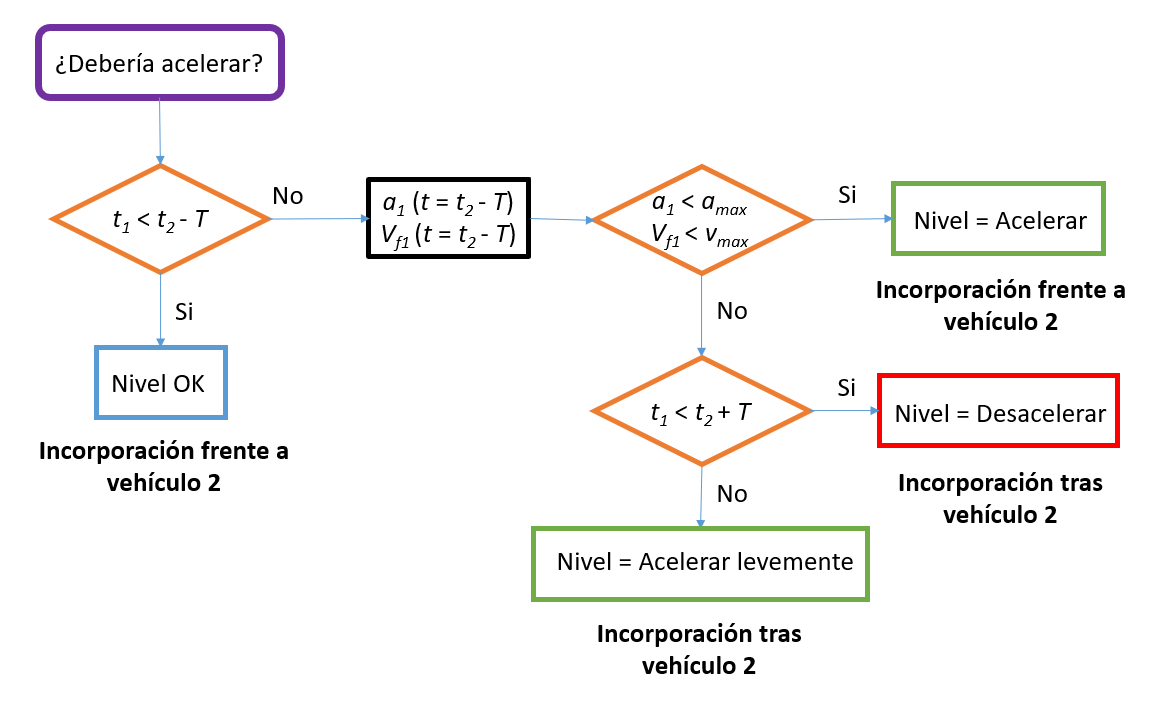
\includegraphics[width=12.5cm]
    {figures/3.7.png}
    \caption{ \label{fig:3.7} Diagrama de flujo del algoritmo de decisión}
\end{figure}

En el primer paso se evalúa si el tiempo que tarda el vehículo 1, \emph{t$_1$}, al final del carril es menor que el del vehículo 2, \emph{t$_2$}, teniendo en cuenta el margen de seguridad establecido, \emph{T}. El tiempo que tarda cada vehículo al final del carril se calcula mediante la ecuación \ref{eq:1}.

\begin{equation}\label{eq:1}
t_1 = \frac{d_i}{v_i}
\end{equation}

 En caso de que el vehículo 1 llegue antes que el vehículo 2, contando con el margen de seguridad, no será necesaria ninguna acción diferente al estado que tienen en ese instante. Si no se cumpliera esta condición, el algoritmo evaluaría si la incorporación se pudiera realizar por delante o por detrás del vehículo 2. En un primer escenario, si el vehículo 1 pudiese adquirir la aceleración necesaria, \emph{a$_1$}, sin superar la aceleración, \emph{a\textsubscript{max}}, ni la velocidad máxima de la vía, \emph{v\textsubscript{max}}, este pasaría delante del vehículo 2. La aceleración necesaria y la velocidad máxima al final del carril vienen dadas por las ecuaciones \ref{eq:2} y \ref{eq:3}.

 \begin{equation}\label{eq:2}
     a_1(t) = \dfrac{d_1-v_1\cdot t}{0.5\cdot t^2}
 \end{equation}

  \begin{equation}\label{eq:3}
      v_{f1}(t) = a_1 \cdot t + v_1
 \end{equation}

En caso contrario, la incorporación debería de hacerse detrás del vehículo 2, comprobando de nuevo la relación de tiempos al final del carril de ambos vehículos junto al margen de seguridad. En función de este resultado, el algoritmo aconsejaría realizar una desaceleración o, si hubiera suficiente distancia, recomendaría acelerar hasta un nivel máximo. Se ha de tener en cuenta que, si existiera un vehículo 3, el bucle se repetiría para verificar que la incorporación entre los vehículos es lo suficientemente segura. 

Al ser el entorno de la maniobra una vía principal tipo autovía o autopista, su velocidad está acotada legalmente a 120 km/h. Dado que a velocidades altas se requieren mayores distancias para frenar, se ha definido un margen de seguridad conservador de 2 segundos en términos de tiempo en base a investigaciones previas y valores utilizados en simuladores de conducción.  De la misma manera, los valores máximos de aceleración y deceleración se han establecido en 2 m/s$^2$ y 4 m/s$^2$ respectivamente. El algoritmo de control presentado posee una baja carga computacional, lo que hace que funcione adecuadamente en tiempo real. El código se implementa en una aplicación móvil con sistema iOS. 

Finalmente, el sistema sugiere al conductor las acciones de acelerar o frenar para realizar la maniobra con seguridad en función de las variables de los vehículos aledaños, respetando en todo momento el margen entre ellos. 

\textbf{\emph{Diseño y localización de la interfaz}}

Los diseños fueron seleccionados en base a la propia experiencia del grupo de investigación en el diseño y validación de interfaces para la conducción segura en dispositivos móviles para aplicaciones anteriores (\cite{jimenez12}; \cite{jimenez16}). Como premisa, se han seguido las Recomendaciones de la Comisión de las Comunidades Europeas de 26 de mayo de 2008, relativas a sistemas de información y comunicación a bordo de vehículos seguros y eficientes (\cite{european}). 

En la figura \ref{fig:3.8a}, se muestran las interfaces propuestas, derivando su diseño del campo de la aeronáutica, en concreto de los variómetros, y presentando la información en forma de conjunto de barras o segmentos circunferenciales. En la figura \ref{fig:3.8b} se puede observar un ejemplo de aplicación de una interfaz sobre el fondo de un navegador de conducción, soportado por un smartphone.

\newpage
\begin{figure}[htbp]
    \centering
    \begin{subfigure}[b]{0.4\linewidth}
        \centering
        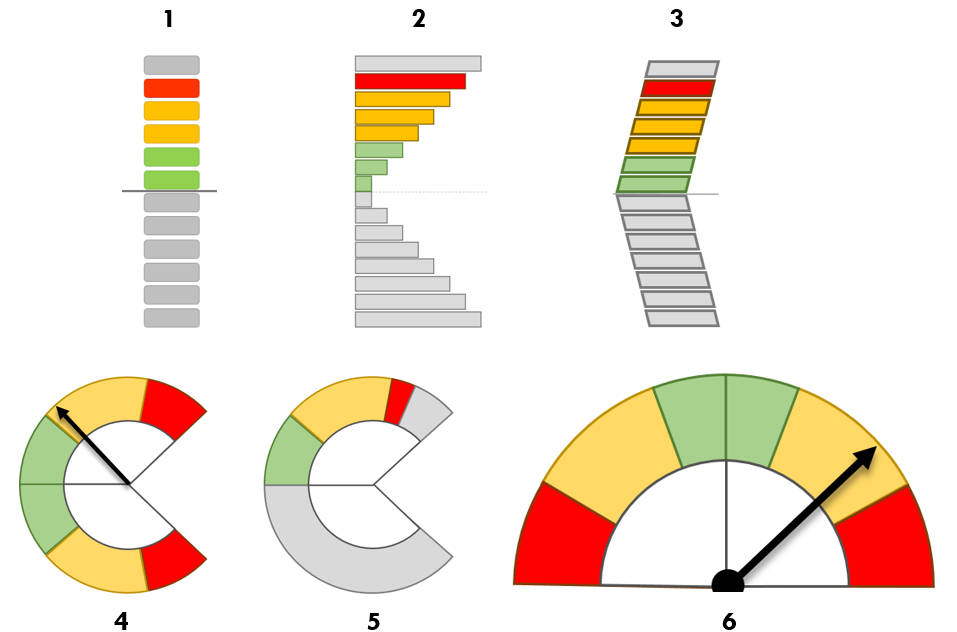
\includegraphics[width=9cm]{figures/3.8a.png}
        \caption{}
        \label{fig:3.8a}
    \end{subfigure}
    \hspace{0.5cm}
    \begin{subfigure}[b]{0.5\linewidth}
        \centering
        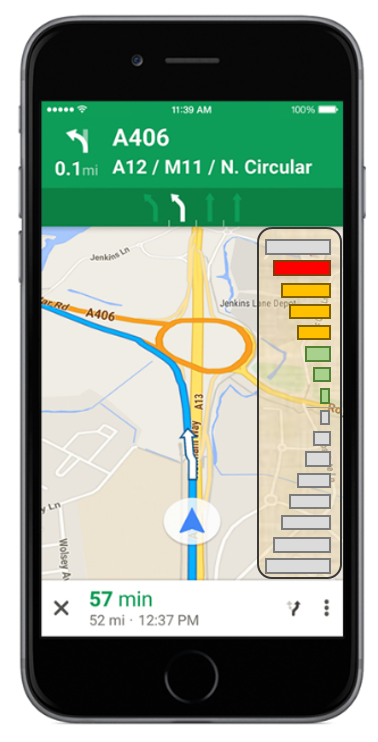
\includegraphics[width=3cm]{figures/3.8b.png}
        \caption{}
        \label{fig:3.8b}
    \end{subfigure}
     \caption{(a) Propuestas de diseños de interfaz. (b) Ejemplo de aplicación en un smartphone }
  \label{fig:3.8}
\end{figure}

La interpretación de los colores es sencilla, cuando más cerca el indicador de la zona roja o más barras aparezcan, mayor aceleración o deceleración se requerirá para realizar la maniobra con seguridad. La interfaz sea ha diseñado para ser configurable por el usuario, pudiendo elegir cuál de los extremos indica acelerar o decelerar, para un entendimiento más intuitivo. La razón de esta característica reside en los resultados obtenidos de una encuesta-sondeo sobre la interpretación de la interfaz 1, elegida por su sencillez. Los participantes contestaron a la siguiente pregunta proyectada junto a la imagen de la interfaz 1:

\emph{``Imagina que vas conduciendo por una carretera y estás a punto de incorporarte a una autopista. Dentro de tu coche se activa un dispositivo de ayuda a la incorporación que te permite conocer si vas muy rápido o muy despacio, pudiendo adecuar la velocidad de tu coche a la situación. Este dispositivo tiene en cuenta diversos factores tales como la velocidad y posición del resto de vehículos y las condiciones de la carretera. Si antes de incorporarte aparece el dispositivo de la siguiente manera, considerarías que tienes que: 1. Frenar, 2. Acelerar''}

Se obtuvieron 209 respuestas para una población de 119 hombres y 90 mujeres, con edades comprendidas de 20 a 90 años (\emph{M} = 43.39, \emph{SD} = 13.34) y una experiencia en conducción de 22.20 años (\emph{SD} = 13.53). Los resultados mostraron respuestas similares en ambas configuraciones, 46.88\% acelerar y 53.11\% frenar.
Finalmente, las interfaces seleccionadas para su evaluación fueron 1, 3 y 6, elegidas gracias al equipo de expertos pertenecientes al Departamento de  Psicobiología y Metodología en Ciencias del Comportamiento de la Universidad Complutense de Madrid. Los criterios de selección fueron los siguientes: la interfaz 1 fue elegida por su sencillez; la interfaz 3 por su similitud con la 1 y 2, además de la ventaja de poder señalar la dirección hacia donde se va a realizar la incorporación; y la interfaz 6 por su similitud con el velocímetro del cuadro de mandos de un vehículo, siendo este diseño familiar para los conductores y a la vez diferente respecto a las anteriores interfaces. 
Su localización se sitúa en la parte inferior del pilar A izquierdo, en base a los resultados obtenidos de los mapas de calor del subapartado \hyperref[3122]{3.1.2.2}.

\subsubsection{3.1.3.2	Metodología}\label{3132}

Un total de 23 sujetos, siendo 11 de ellos hombres y 12 mujeres, participaron en el estudio de evaluación de interfaces en un simulador de conducción. La edad de los participantes esta comprendidas entre los 18 y los 53 años (\emph{M} = 28, \emph{SD} = 9.4). Su experiencia media al volante fue de 8.4 años y la desviación estándar de 9.4. De manera general, los participantes declararon conducir regularmente un vehículo turismo.

El estudio de las interfaces y los ensayos en el simulador fue fruto del grupo de investigación, en colaboración con el Departamento de  Psicobiología y Metodología en Ciencias del Comportamiento de la Universidad Complutense de Madrid, donde se ubicaba el propio simulador de conducción. Dicho simulador se encuentra instalado dentro de una cabina de Faraday. Se proyectaron tres grabaciones de 5 minutos para cada una de las interfaces, donde los participantes realizaron la tarea de conducción simulada mediante un volante y un conjunto de pedales de aceleración y freno. El simulador disponía de cambio de marchas automático. 

Previo al inicio del ensayo los participantes eligieron la configuración de funcionamiento que les resultaba más intuitiva y se les pidió que condujeran de la forma más natural posible siguiendo las instrucciones de la interfaz. Al finalizar cada grabación respondieron a las encuestas de aceptación, usabilidad del sistema y esfuerzo mental sobre la interfaz. Finalmente, también respondieron a preguntas sobre información demográfica y si implementarían este sistema en su teléfono móvil si fuera gratuito.

El diseño de la investigación fue intrasujeto, donde todos los participantes pasaron por las mismas tres situaciones experimentales, una para cada tipo de interfaz, y las interfaces aparecieron de forma contrabaleanceada para paliar los efectos de orden. La duración media de cada sesión fue de 20 minutos en total. Las condiciones analizadas son las mismas que las descritas en el subapartado \hyperref[3121]{3.1.2.1.}, diferenciando los intervalos de incorporación del resto del ensayo (línea base) a raíz de la primera mirada al retrovisor. 

El análisis de la mirada también se realizó con el sistema de seguimiento ocular empleado en el subapartado \hyperref[3121]{3.1.2.1.}, adquiriendo las variables descritas anteriormente. 
Para cada interfaz se midieron las siguientes variables: A) Aceptación del sistema (Satisfacción, Utilidad y Usabilidad); B) Esfuerzo mental (a través de una medida subjetiva, la Escala de Valoración del Esfuerzo Mental (\gls{rsme}) y de la medida fisiológica de la dilatación pupilar); C) Medidas oculares (tiempo total mirando la interfaz, número y duración media de fijaciones) y medidas del seguimiento de la interfaz (porcentaje de seguimiento de la interfaz en velocidad y dirección); D) Mapas de calor.
Después de cada simulación, donde se realizaba la tarea de conducción simulada para un modelo de interfaz, los participantes respondían al cuestionario de Aceptación de Sistemas de \textcite{vanderlaan}. Este cuestionario constó de nueve ítems de 5 respuestas, que puntuaron para las escalas de utilidad del sistema y satisfacción entre -2 y +2. Posteriormente, los participantes respondieron a la Escala de Usabilidad del Sistema (\cite{brooke}), puntuada entre 0 y 100, y a la Escala de Valoración del Esfuerzo Mental \gls{rsme} (\cite{zijlstra};) cuyos valores se encuentran entre 0-150 puntos. Al final de las 3 simulaciones de conducción, también respondieron a algunas preguntas sobre información demográfica, así como si implementarían o no la aplicación en su móvil si fuera gratuita. 
Para cada diseño, se realizó un análisis de varianzas (\gls{anova}) unifactorial de medidas repetidas con el software SPSS v26. El ajuste de las comparaciones por pares se realizó mediante el método de Bonferroni. 

\subsubsection{3.1.3.3 Resultados}\label{3133}

\textbf{\emph{Medidas de satisfacción, utilidad y usabilidad}}

En las encuestas de aceptación del sistema se encontraron diferencias estadísticamente significativas en la evaluación de los conductores para los distintos tipos de interfaz en relación con la satisfacción, utilidad y usabilidad, con valores de \emph{F} (2;44) = 7.7, \emph{p} = 0.001, $\eta^2$ = 0.26; \emph{F} (2;44) = 3.53, \emph{p} = 0.038, $\eta^2$ = 0.14 y \emph{F} (2;44) = 9.2, \emph{p} < 0.001, $\eta^2$ = 0.3, respectivamente. Las interfaces 1 y 3 fueron evaluadas como más satisfactorias, útiles y utilizables que la interfaz 6 (Figura \ref{fig:3.9}).

\newpage
\begin{figure}[h]
  \centering
  \begin{subfigure}[b]{0.45\textwidth}
    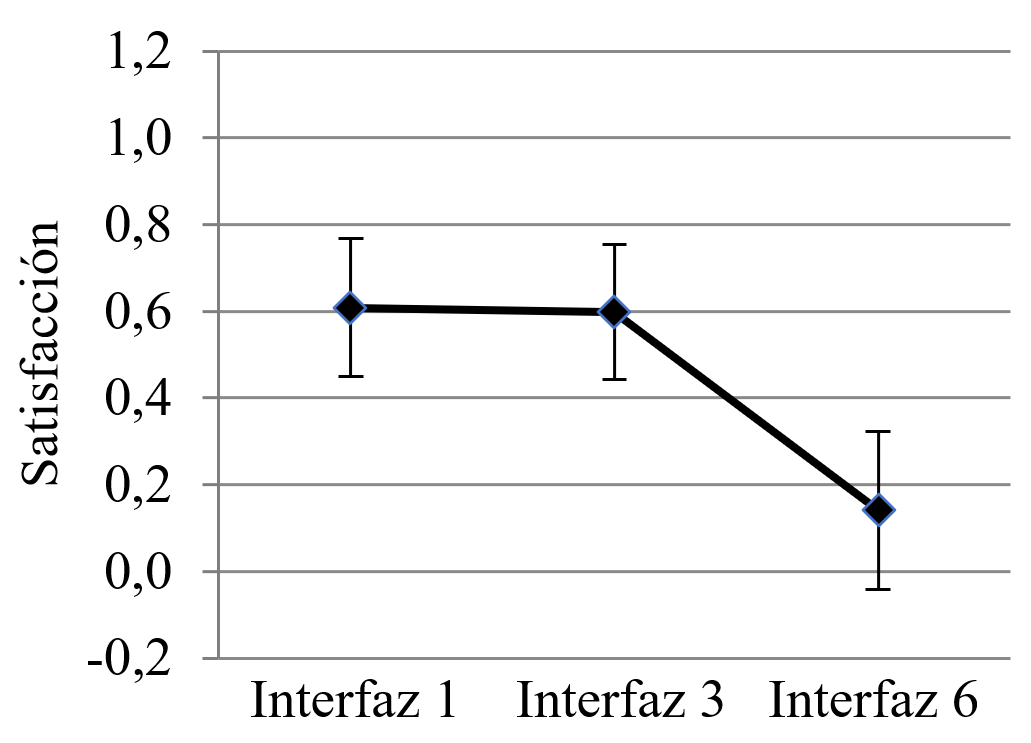
\includegraphics[width=\textwidth]{figures/3.9a.png}
    \caption{}
    \label{fig:3.9a}
  \end{subfigure}
  \hfill
  \begin{subfigure}[b]{0.45\textwidth}
    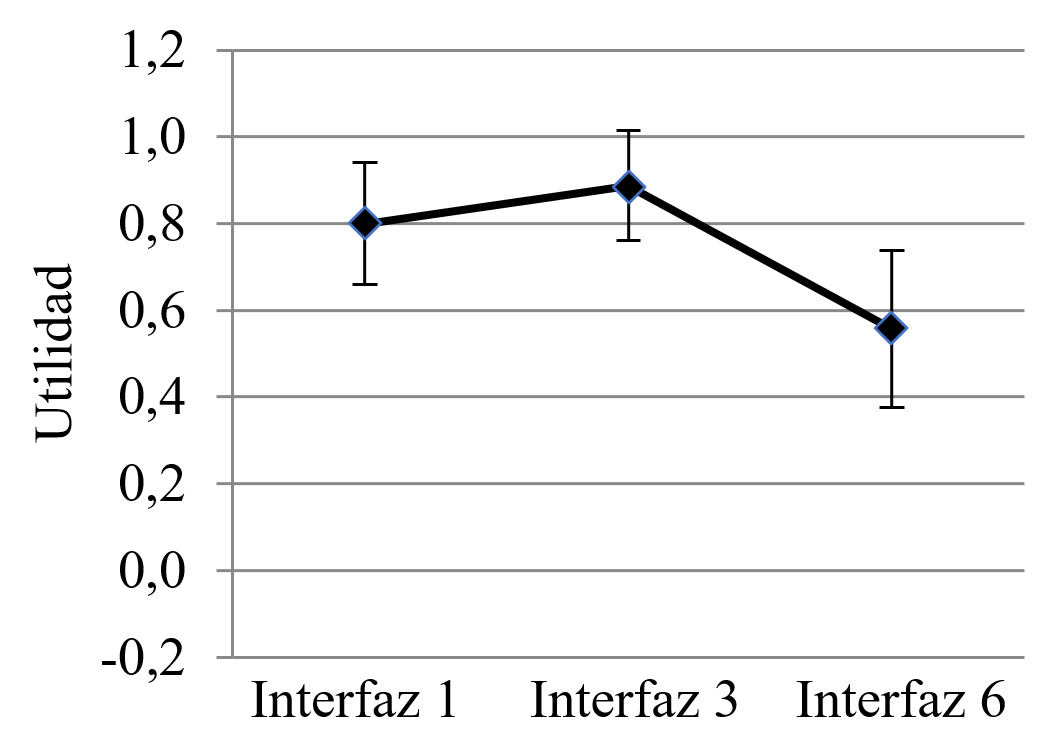
\includegraphics[width=\textwidth]{figures/3.9b.png}
    \caption{}
    \label{fig:3.9b}
  \end{subfigure}
  \begin{subfigure}[b]{0.45\textwidth}
    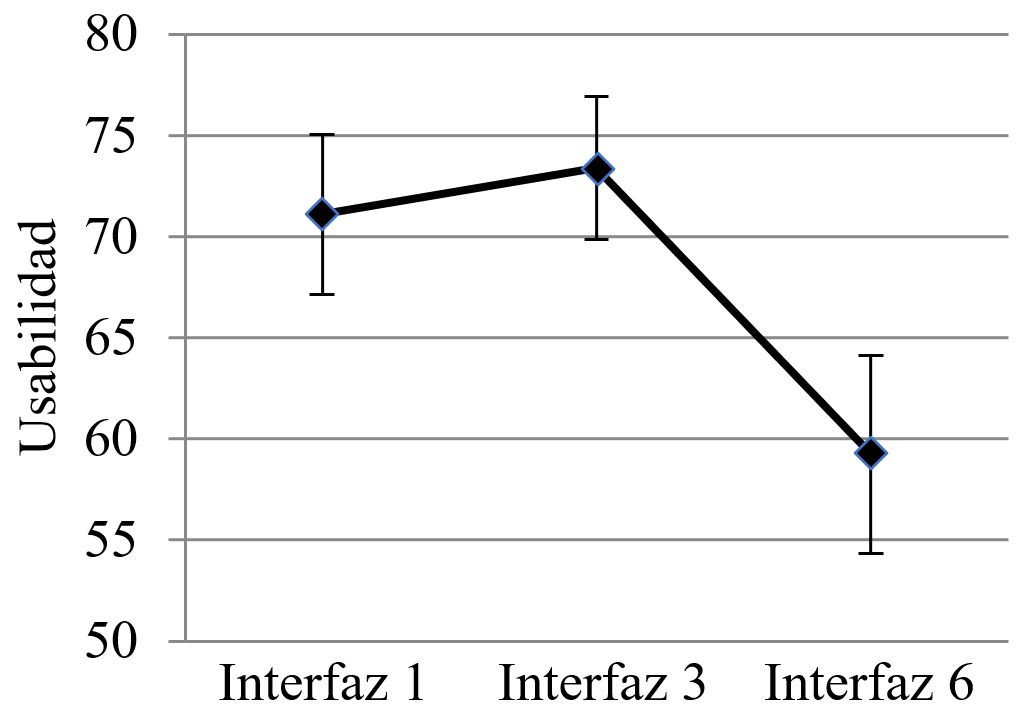
\includegraphics[width=\textwidth]{figures/3.9c.png}
    \caption{}
    \label{fig:3.9c}
  \end{subfigure}
  \caption{Media y error estándar de (a) Satisfacción (b) Utilidad (c) Usabilidad}
  \label{fig:3.9}
\end{figure}

\textbf{\emph{Medidas de esfuerzo mental}}

El esfuerzo mental fue evaluado mediante dos parámetros, uno subjetivo, representado por la Escala de Valoración del Esfuerzo Mental \gls{rsme}, y otro fisiológico utilizando el diámetro de la pupila. Los resultados relativos a la escala de esfuerzo mental mostraron diferencias significativas entre las interfaces 1 y 3 con la interfaz 6 (\emph{F} (2;44) = 5.57, \emph{p} = 0.007, $\eta^2$ = 0.2), siendo valorada esta última como más costosa de seguir que las anteriores. No se encontraron diferencias significanticas entre las interfaces 1 y 3. Los resultados pueden verse en la figura \ref{fig:3.10}.

\newpage
\begin{figure}[h]
    \centering
    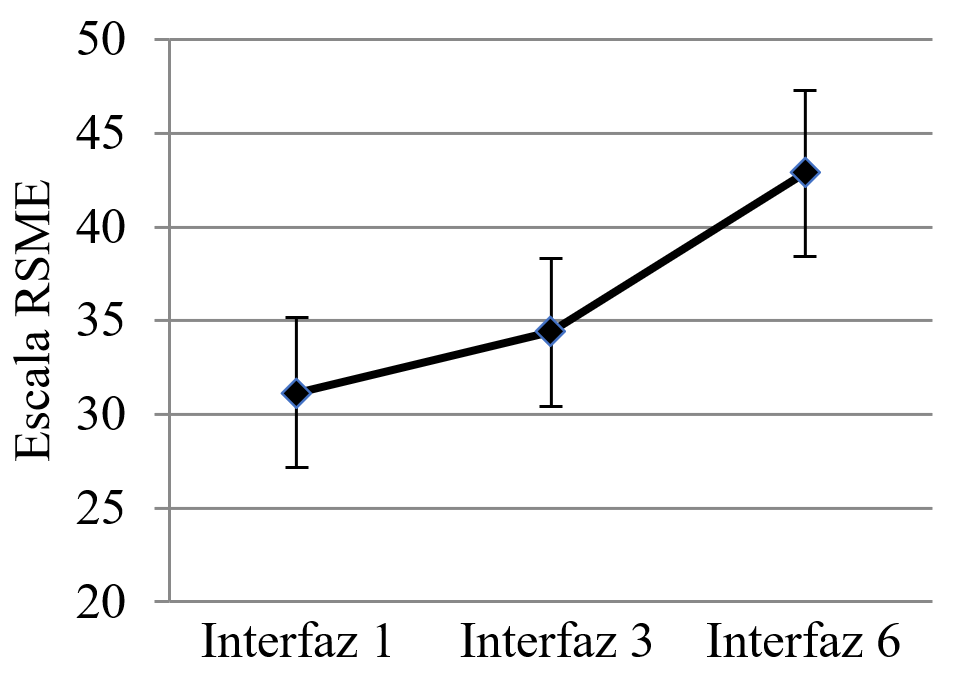
\includegraphics[width=7cm]
    {figures/3.10.png}
    \caption{ \label{fig:3.10} Media y error estándar de la Escala de Valoración de Esfuerzo Mental (\gls{rsme})}
\end{figure}

Para la variable fisiológica diámetro de la pupila, se encontraron diferencias estadísticamente significativas entre las situaciones sin interfaz o de línea base e interfaz activa (Figura \ref{fig:3.11}), con los valores de \emph{F} (3;57) = 19.68, \emph{p} < 0.001, $\eta^2$ = 0.51 para la pupila izquierda, y \emph{F} (3;57) = 17.31, \emph{p} < 0.001, $\eta^2$ = 0.48 para la pupila derecha. No obstante, no se encontraron diferencias entre las diferentes interfaces. Cabe añadir que el diámetro de la pupila no se vio afectado por los cambios lumínicos ya que las pruebas se realizaron en un laboratorio en condiciones estables. 

\begin{figure}[h]
  \centering
  \begin{subfigure}[b]{0.45\textwidth}
    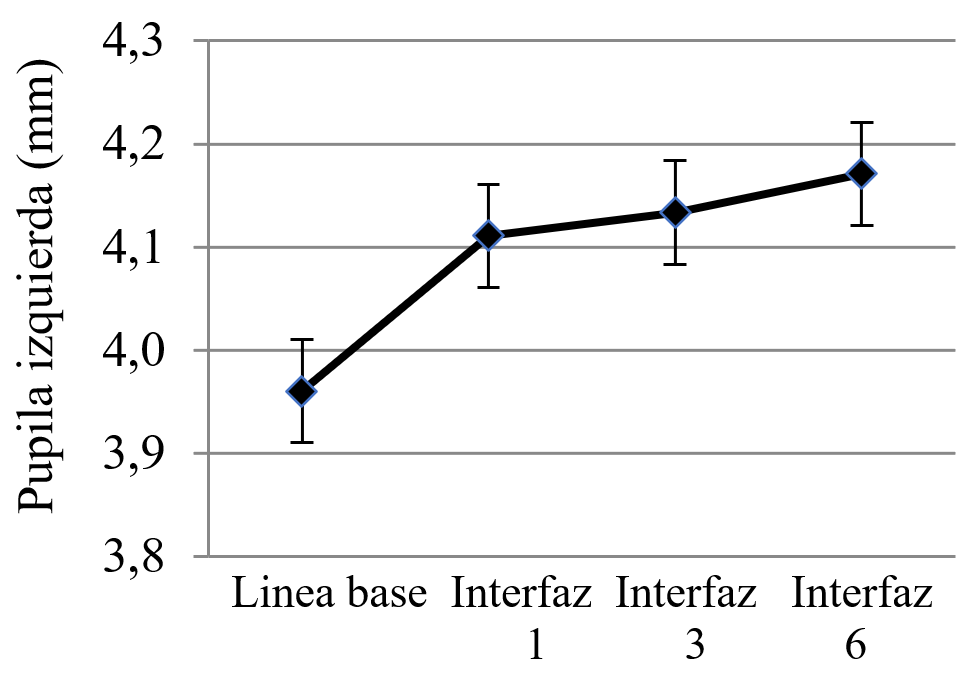
\includegraphics[width=\textwidth]{figures/3.11a.png}
    \caption{}
    \label{fig:3.11a}
  \end{subfigure}
  \hfill
  \begin{subfigure}[b]{0.45\textwidth}
    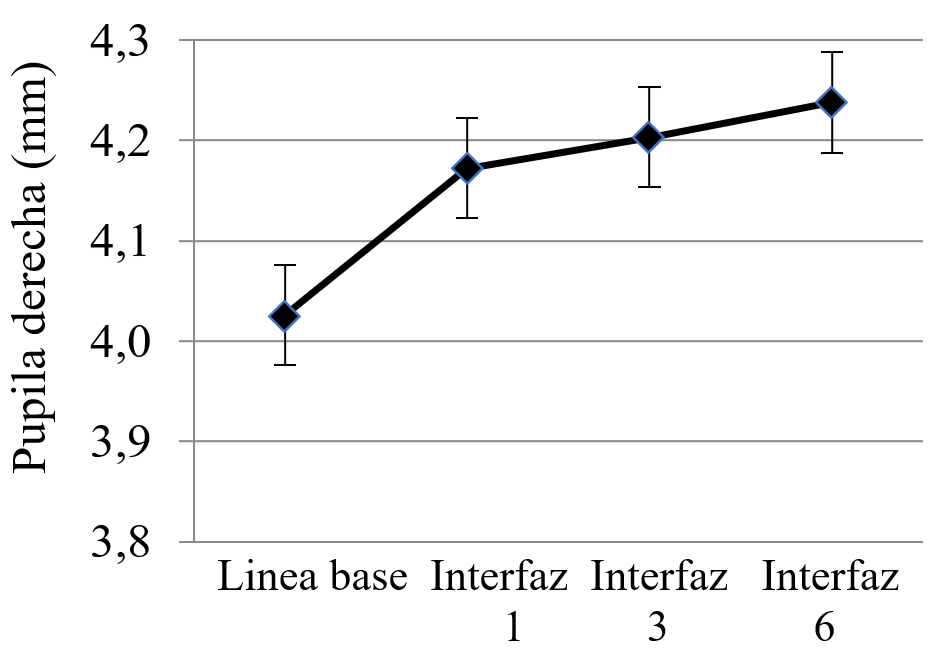
\includegraphics[width=\textwidth]{figures/3.11b.png}
    \caption{}
    \label{fig:3.11b}
  \end{subfigure}
  \caption{Media y error estándar del diámetro de las pupilas en la ausencia/presencia de las interfaces: (a) pupila izquierda, (b) pupila derecha}
  \label{fig:3.11}
\end{figure}

\textbf{\emph{Medidas oculares y seguimiento de la interfaz}}

En cuanto a otras medidas oculares utilizadas, como miradas, fijaciones y seguimiento de la interfaz en velocidad y giro de volante, no se encontraron diferencias estadísticamente significativas en función del diseño de la interfaz. En la tabla \ref{tab:3.8} se muestra un resumen del análisis de estas medidas durante las incorporaciones con los valores de la media, el error estándar y los resultados de la prueba \gls{anova}, cuyos resultados no son significativos.

\newpage
\begin{table}[h]
\centering
\begin{tabular}{rcc|cc|cc|cc}
\multirow{2}{*}{\textbf{Variable}} & \multicolumn{2}{c|}{\textbf{Interfaz 1}} & \multicolumn{2}{c|}{\textbf{Interfaz 3}} & \multicolumn{2}{c|}{\textbf{Interfaz 6}} & \multirow{2}{*}{\textbf{F}} & \multirow{2}{*}{\textbf{\emph{p}-valor}} \\ \cline{2-7}
                                   & \textit{M}         & \textit{SE}         & \textit{M}         & \textit{SE}         & \textit{M}         & \textit{SE}         &                             &                                   \\ \hline
TTM (s)*                           & 3.78               & 0.42                & 4.71               & 0.61                & 4.11               & 0.51                & 2.54                        & 0.09                              \\ \hline
Número de fijaciones               & 8.03               & 0.56                & 8.09               & 0.47                & 8.11               & 0.59                & 0.01                        & 0.98                              \\ \hline
Duración fijaciones (ms)           & 406                & 25                  & 468                & 40                  & 447                & 34                  & 2.04                        & 0.15                              \\ \hline
PTV*                               & 49\%               & 0.005               & 50\%               & 0.005               & 49\%               & 0.006               & 0.16                        & 0.85                              \\ \hline
PTVT*                              & 73\%               & 0.03                & 71\%               & 0.05                & 74\%               & 0.04                & 0.07                        & 0.80                              \\ \hline
\end{tabular}%
\caption{Media y error estándar de las medidas oculares y seguimiento de la interfaz}
\label{tab:3.8}
\end{table}

\textbf{\emph{Mapas de calor}}

Por último, se muestra a nivel visual un ejemplo de los mapas de calor de cada una de las interfaces ensayadas (Figura \ref{fig:3.12}). Relacionado con los resultados anteriores, se observa que los conductores dividen su atención hacia la interfaz, siendo este con el espejo retrovisor izquierdo y el carril central, uno de los tres puntos calientes característicos.

\begin{figure}[h]
  \centering
  \begin{subfigure}[b]{0.4\textwidth}
    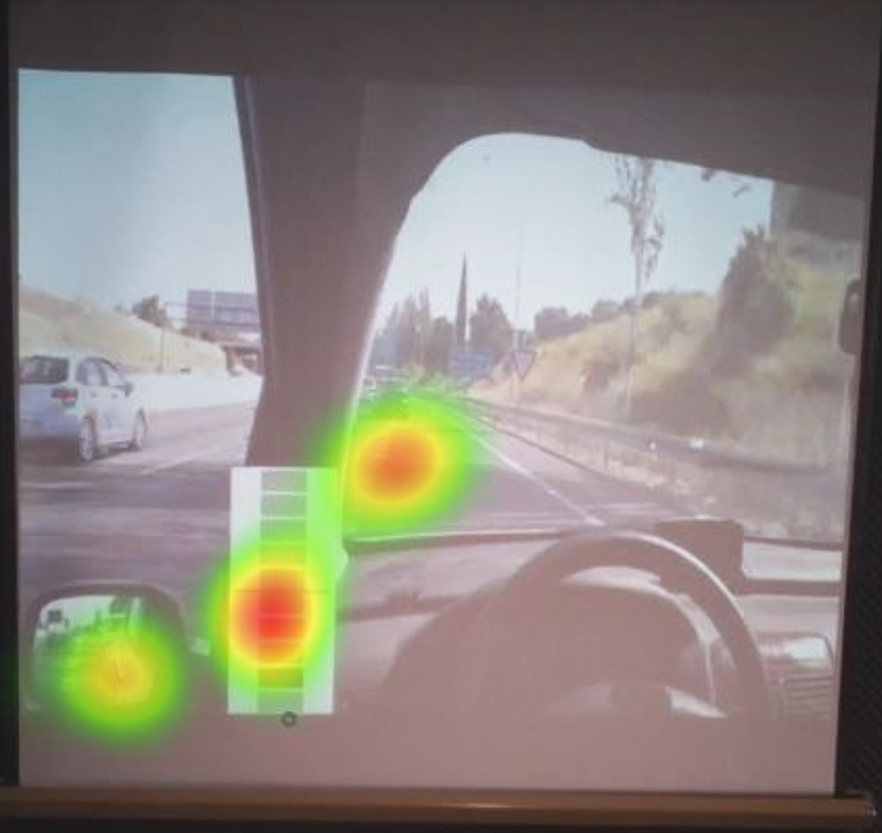
\includegraphics[width=\textwidth]{figures/3.12a.png}
    \caption{}
    \label{fig:3.12a}
  \end{subfigure}
  \hfill
  \begin{subfigure}[b]{0.4\textwidth}
    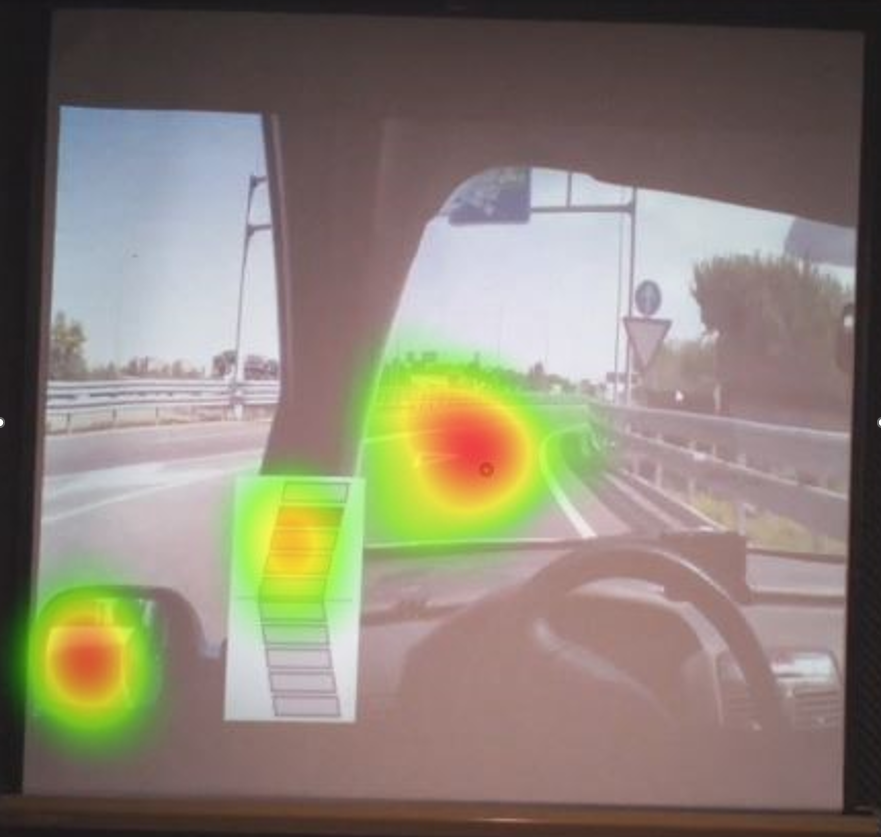
\includegraphics[width=\textwidth]{figures/3.12b.png}
    \caption{}
    \label{fig:3.12b}
  \end{subfigure}
  \begin{subfigure}[b]{0.4\textwidth}
    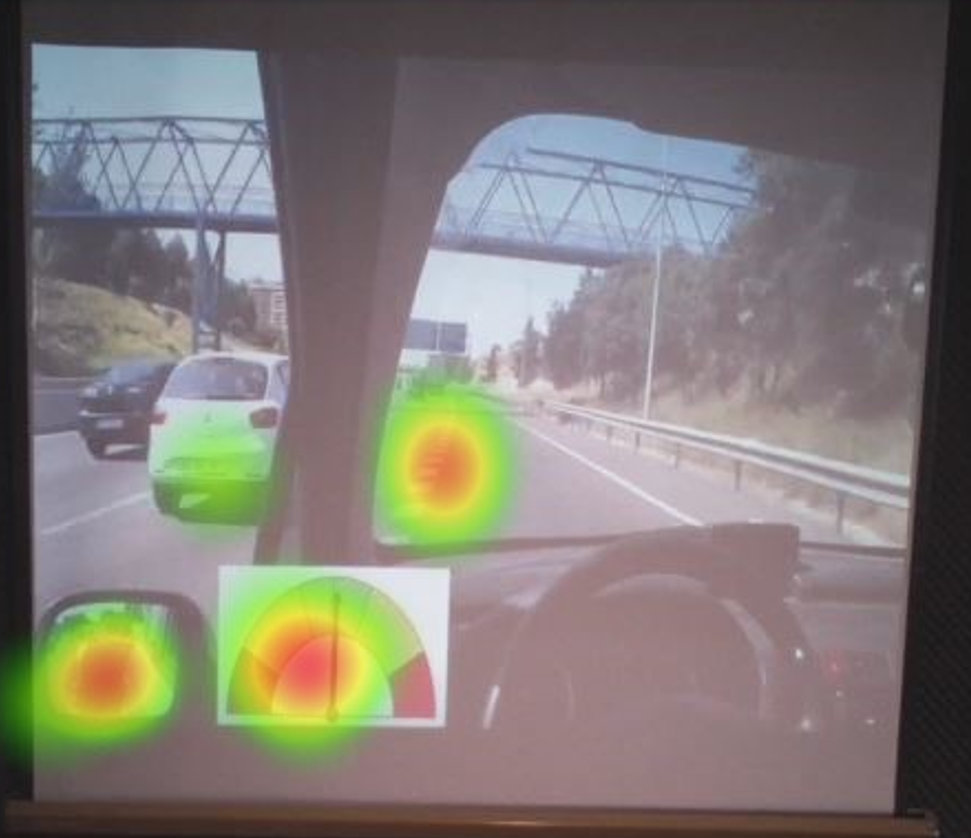
\includegraphics[width=\textwidth]{figures/3.12c.png}
    \caption{}
    \label{fig:3.12c}
  \end{subfigure}
  \caption{Mapas de calor para cada una de las interfaces durante una incorporación: (a) Interfaz 1, (b) Interfaz 3, (c) Interfaz 6}
  \label{fig:3.12}
\end{figure}

\subsubsection{3.1.3.4 Discusión}\label{3134}

Tres diseños de interfaz para un sistema de ayuda a la incorporación fueron evaluados en un simulador de conducción, atendiendo a encuestas sobre aceptación por parte del usuario y a variables atencionales del conductor. A nivel estadístico se encontraron diferencias en la aceptación por parte de los usuarios de las interfaces 1 o 3 frente a la interfaz 6, valorando las dos primeras como más satisfactorias, usables y útiles que la interfaz 6. Estas características son fundamentales cuando se desarrolla una nueva tecnología en los vehículos, ya que resulta improductivo invertir esfuerzos en el diseño y la construcción de un sistema si después no es utilizado o incluso se desactiva.

Considerando conjuntamente los resultados de las dos variables de esfuerzo mental, diámetro pupilar y \gls{rsme}, se puede concluir que seguir la interfaz 6 supone mayor esfuerzo que seguir las interfaces 1 y 3. Los resultados de \gls{rsme} mostraron diferencias significativas, y a pesar de que no se encontraron estas mismas diferencias para los diámetros pupilares entre interfaces, se puede percibir que sigue la misma tendencia que la escala \gls{rsme}. No obstante, sí se encontraron diferencias en la dilatación pupilar entre línea base y aparición de cualquier interfaz, numéricamente en torno al 3.5\%, mostrando de nuevo que el esfuerzo mental es mayor en la situación de incorporación. 

Otras medidas oculares mostraron similitud en los resultados recogidos entre interfaces, sin destacar ninguna diferencia significativa. Junto a los mapas de calor, se observa el correcto funcionamiento que han realizado los participantes durante el experimento, siendo el área de la interfaz junto a la del espejo izquierdo y el carril central, uno de los tres puntos calientes más mirados durante una incorporación. Tampoco se apreciaron efectos de orden ante la aparición de las interfaces, gracias a su aparición contrabalanceada.

Teniendo en cuenta todos los resultados, se descarta la interfaz 6 para la siguiente fase y se elige la interfaz 3 para implementarla en el sistema final, debido a que obtuvo resultados similares a la interfaz 1, pero aportando más información, como la dirección de la maniobra. En el siguiente estudio se realizan ensayos en conducción real con la interfaz propuesta, evaluando el funcionamiento del sistema mediante variables atencionales y encuestas de aceptación y carga mental.

\subsection{Validación de sistema de asistencia en incorporaciones en ensayos reales}\label{314}

Como se ha podido ver en fases anteriores, las variables atencionales del conductor proporcionan información sobre su estado ante diferentes eventos al igual que la aceptación de sistemas avanzados de ayuda o asistencia a la conducción (\gls{adas}). En el anterior estudio se propuso un sistema de ayuda a la incorporación mediante la generación de avisos basados en comunicaciones \gls{v2v}. En este estudio se implementa dicho sistema en conducción real, realizado ensayos bajo las mismas condiciones que en el simulador de conducción del subapartado \hyperref[313]{3.1.3.}. De la misma manera se registran los datos del seguimiento ocular, aceptabilidad y esfuerzo mental, añadiendo el cuestionario NASA-TLX sobre el índice de carga de la tarea. 

\subsubsection{3.1.4.1	Metodología}\label{3141}

Trece participantes, 2 de ellos mujeres, participaron en este estudio con edades comprendidas entre los 24 y los 43 años (\emph{M} = 31.53, \emph{SD} = 6.35). Su experiencia media al volante fue de 11.53 años (\emph{SD} = 6.59). 

Las pruebas de conducción real se realizaron en un tramo de la autovía M-45, situado en la zona sureste de Madrid, coincidiendo con tres zonas de incorporación señalizadas. Antes de realizar las pruebas reales, los conductores completaron la primera parte del cuestionario de carga de tareas de la NASA, en el que evaluaba subjetivamente la carga de trabajo de una tarea. 

Previo al inicio del ensayo los participantes eligieron la configuración de funcionamiento que les resultaba más intuitiva y se les pidió que condujeran de la forma más natural posible siguiendo las instrucciones de la interfaz. A continuación, se realizaron las pruebas con los vehículos instrumentados, el sistema de seguimiento ocular y el sistema de asistencia para ayudarles en las maniobras de incorporación.  Al finalizar la conducción realizaron la segunda parte del cuestionario de carga de tareas NASA junto a las encuestas de aceptación, usabilidad del sistema y esfuerzo mental sobre la interfaz. Finalmente, también respondieron a preguntas sobre información demográfica y si implementarían este sistema en su teléfono móvil si fuera gratuito. La duración media de cada sesión fue de aproximadamente quince minutos de conducción y cinco minutos más para responder a las escalas tras el ensayo. 

Las condiciones analizadas son las mismas que las descritas en el subapartado \hyperref[3121]{3.1.2.1.}, diferenciando los intervalos de incorporación del resto del ensayo (línea base) en base a la primera mirada al retrovisor. 

En esta última parte, el vehículo que realiza la incorporación fue instrumentado con el sistema de ayuda a la incorporación desarrollado en el subapartado \hyperref[313]{3.1.3}. El sistema fue soportado en un teléfono inteligente ubicado en la parte inferior del pilar A izquierdo del vehículo, tal y como se justifica en el subapartado \hyperref[3122]{3.1.2.2.} Las únicas entradas que necesita son los parámetros de posición y velocidad de ambos vehículos al final del carril, recogidos mediante un y enviados a través de módulos de comunicaciones desarrollados por INSIA y situados en cada uno de los vehículos (Figura \ref{fig:3.13}).

\begin{figure}[h]
    \centering
    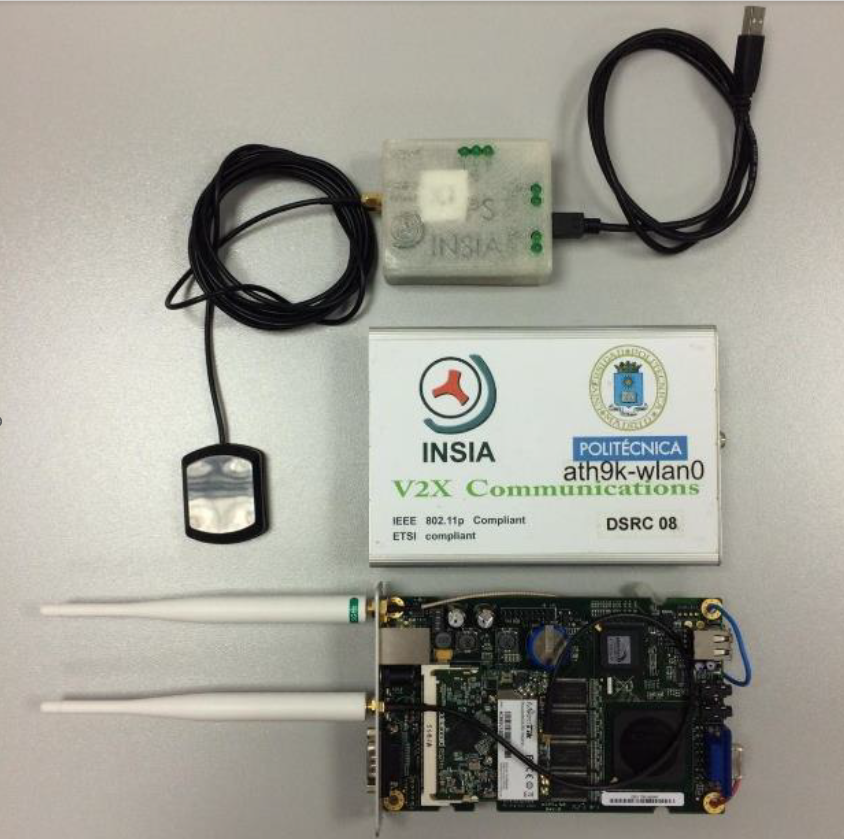
\includegraphics[width=8cm]
    {figures/3.13.png}
    \caption{ \label{fig:3.13} Módulo de comunicaciones y GNSS desarrollados por INSIA}
\end{figure}

Todos los vehículos implicados dispusieron de un módulo de comunicaciones Vehículo-a-vehículo (\gls{v2v}) acompañado de un Sistema Global de Navegación por Satélite (\gls{gnss}) de donde obtienen información sobre su posición y velocidad de ambos vehículos. Esta información llega desde los módulos vía WiFi a la aplicación de asistencia en incorporaciones, que genera avisos visuales al conductor (Figura \ref{fig:3.14}).

\newpage
\begin{figure}[h]
    \centering
    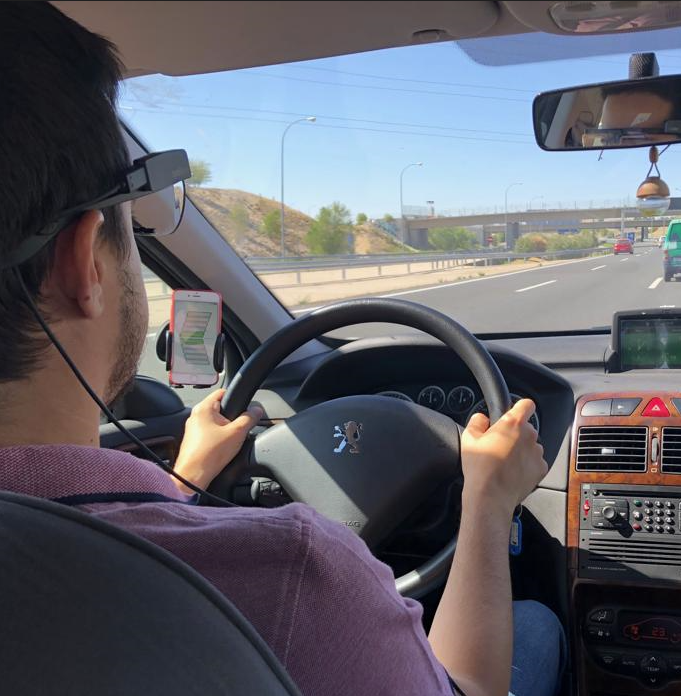
\includegraphics[width=8cm]
    {figures/3.14.png}
    \caption{ \label{fig:3.14} Aplicación de asistencia en incorporaciones en tráfico real}
\end{figure}

El uso de este sistema no condiciona la conducción en caso de ser ignorado y funciona solo como interfaz hombre-máquina, sin necesidad de ser manipulado durante la conducción. El análisis de la mirada también se realizó con el sistema de seguimiento ocular empleado en el subapartado \hyperref[3121]{3.1.2.1.}, al igual que el vehículo utilizado en la conducción. 

Para evaluar el funcionamiento del sistema de ayuda a la conducción se registraron las siguientes medidas al igual que en el subapartado \hyperref[313]{3.1.3.}: A) Aceptación del sistema (Satisfacción, Utilidad y Usabilidad); B) Esfuerzo mental (a través de dos medidas subjetivas, la Escala de Valoración del Esfuerzo Mental \gls{rsme} y el Índice de Carga de Tareas NASA-TLX; y de una medida fisiológica, la dilatación pupilar). 

Las encuestas utilizadas se encuentran descritas en el subapartado \hyperref[3132]{3.1.3.2.}, a excepción del cuestionario de carga de tareas que complementa al de esfuerzo mental. Este cuestionario es el Índice de Carga de Tareas de la Administración Nacional de la Aeronáutica y del Espacio (NASA-TLX) (\cite{hart}), el cual es ampliamente utilizado dado los sólidos argumentos alcanzados en investigación de factores humanos (\cite{pauzie}; \cite{rubio}). También se utiliza hoy en día para evaluar la carga de trabajo subjetiva y el esfuerzo cognitivo para una tarea proyectada en una \gls{hmi}, como en \textcite{pereira}, \textcite{matthews} y \textcite{papis}. Los cuestionarios de esfuerzo mental (\gls{rsme}) y carga de tareas, o de trabajo, (NASA-TLX) pueden resultar equivalentes por la terminología, pero evalúan desde diferentes enfoques la cognición frente a una tarea. El cuestionario de esfuerzo mental consiste en una escala unifactorial donde se puntúa cuanto esfuerzo requiere una tarea tras la realización de la misma. El cuestionario de carga de tareas evalúa las dimensiones de carga de trabajo, entre las que se encuentran demanda mental, demanda física, exigencia temporal, rendimiento, esfuerzo y frustración, analizando cada dimensión por pares antes y después de realizar la tarea. Algunas investigaciones utilizan ambas escalas para obtener un resultado más completo en sus estudios (\cite{sartang}; \cite{longo})

Los resultados de dilatación pupilar se analizaron mediante una prueba de rangos con signo de Wilcoxon para muestras pareadas con el fin de verificar si existen diferencias estadísticamente significativas. Por último, se calculó el coeficiente de correlación de Pearson o \emph{r} con objeto de hallar relaciones entre las variables obtenidas de este estudio. Los análisis estadísticos se realizaron con el software estadístico SPSS v26.

\subsubsection{3.1.4.2 Resultados}\label{3142}
\textbf{\emph{Medidas de satisfacción, utilidad y usabilidad}}

Los resultados de aceptación del sistema de ayuda en conducción real se resumen a continuación. En la tabla \ref{tab:3.9} se muestra la media y el error estándar junto a su correspondiente escala, observándose que las puntuaciones recogidas se encuentran por encima del valor medio. 


\begin{table}[h]
\centering
\begin{tabular}{rclcc}
               & \multicolumn{2}{c}{\textbf{Satisfacción}} & \textbf{Utilidad} & \textbf{Usabilidad} \\ \hline
Media          & \multicolumn{2}{c}{0.3269}                & 0.1385            & 65.193              \\ \hline
Error estándar & \multicolumn{2}{c}{0.1843}                & 0.1623            & 4.7910              \\ \hline
Escala         & \multicolumn{2}{c}{-2 ; +2}               & -2 ; +2           & 0 ; 100             \\ \hline
\end{tabular}
\caption{Media, error estándar y escala de satisfacción, utilidad y usabilidad}
\label{tab:3.9}
\end{table}

A pesar de que los resultados son meramente descriptivos, se puede considerar que los usuarios valoran positivamente el sistema de asistencia.

\textbf{\emph{Medidas de esfuerzo mental}}

El esfuerzo mental que pueda suponer atender al sistema durante la maniobra de incorporación se ha analizado mediante la Escala de Valoración del Esfuerzo Mental \gls{rsme} y el Índice de Carga de Tareas NASA-TLX. En la tabla \ref{tab:3.10} se exponen los resultados de la media y el error estándar junto a sus escalas.

\begin{table}[h]
\centering
\begin{tabular}{rllc}
               & \multicolumn{2}{l}\textbf{\gls{rsme}} & \textbf{NASA-TLX} \\ \hline
Media          & \multicolumn{2}{l}{37.6923}       & 0.1385            \\ \hline
Error estándar & \multicolumn{2}{l}{4.6207}        & 0.1623            \\ \hline
Escala         & \multicolumn{2}{l}{0 ; 150}       & 0 ; 100           \\ \hline
\end{tabular}
\caption{Media, error estándar y escala de \gls{rsme} y NASA-TLX}
\label{tab:3.10}
\end{table}

Se advierte que ambas variables se encuentran por debajo del valor medio, siendo la carga mayor que el esfuerzo. Dado que no es posible comparar con otros sistemas, la puntuación más fiable en este campo sería NASA-TLX, ya que además se basa en las puntuaciones antes y después del uso del sistema. 

En cuanto a las medidas de seguimiento ocular, no se encontraron diferencias estadísticamente significativas en el tamaño de la pupila durante las incorporaciones en función de la aparición del sistema de asistencia, ni para la pupila del ojo izquierdo ni para la del derecho, \emph{Z} = -0.594, \emph{p} = 0.552 y \emph{Z} = -0.664, \emph{p} = 0.507, respectivamente. Estos resultados apoyan la hipótesis de que en ambas situaciones la carga es la misma y que el uso del sistema de asistencia no implica un sobreesfuerzo para los conductores, probablemente debido al estrés propio que requiere la situación de incorporación (Tabla \ref{tab:3.11}).

\newpage
\begin{table}[]
\centering
\begin{tabular}{rcccc}
               & \multicolumn{2}{c}{\textbf{\begin{tabular}[c]{@{}c@{}}Diámetro de   pupila\\  izquierda\end{tabular}}} & \multicolumn{2}{c}{\textbf{\begin{tabular}[c]{@{}c@{}}Diámetro de   pupila\\  derecha\end{tabular}}} \\ \cline{2-5} 
\textit{}      & \textit{Con \gls{adas}}                                  & \textit{Sin \gls{adas}}                                 & \textit{Con \gls{adas}}                                 & \textit{Sin \gls{adas}}                                \\ \hline
Media          & 2.2754                                             & 2.2780                                            & 2.2915                                            & 2.3070                                           \\ \hline
Error estándar & 0.045                                              & 0.055                                             & 0.045                                             & 0.054                                            \\ \hline
\end{tabular}
\caption{Media y error estándar del diámetro de la pupila izquierda y derecha durante la incorporación con y sin el sistema de asistencia (\gls{adas})}
\label{tab:3.11}
\end{table}

\textbf{\emph{Correlaciones entre variables}}

Las posibles relaciones lineales entre las variables obtenidas de todos los participantes fueron estudiadas mediante el coeficiente de correlación de Pearson (\emph{r}). Se realizó un análisis entre todas las variables adquiridas durante el ensayo de conducción real, encontrando correlaciones estadísticamente significativas en algunas de ellas (Tabla \ref{tab:3.12}). 


\begin{table}[h]
\centering
\begin{tabular}{rcccc}
                                  & \textbf{Usabilidad}                                                  & \textbf{\gls{rsme}}                                                     & \textbf{NASA-TLX}                                               & \textbf{Utilidad}                                                     \\ \hline
Satisfacción                      & \begin{tabular}[c]{@{}c@{}}\emph{r} = 0.84\\ \emph{p} \textless 0.001\end{tabular} & \begin{tabular}[c]{@{}c@{}}\emph{r} = -0.56\\    \emph{p} = 0.048\end{tabular}  & \cellcolor[HTML]{C9C9C9}\textit{}                               & \cellcolor[HTML]{C9C9C9}\textit{}                            \\ \hline
Diámetro de la   pupila           & \cellcolor[HTML]{C9C9C9}                                             & \begin{tabular}[c]{@{}c@{}}\emph{r} = 0.66\\    \emph{p} =   0.014\end{tabular} & \cellcolor[HTML]{C9C9C9}                                        & \cellcolor[HTML]{C9C9C9}                                     \\ \hline
Número de   fijaciones            & \cellcolor[HTML]{C9C9C9}                                             & \cellcolor[HTML]{C9C9C9}                                          & \begin{tabular}[c]{@{}c@{}}\emph{r} = 0.57\\    \emph{p} = 0.042\end{tabular} & \cellcolor[HTML]{C9C9C9}                                     \\ \hline
Número de   miradas a la interfaz & \cellcolor[HTML]{C9C9C9}                                             & \cellcolor[HTML]{C9C9C9}                                          & \cellcolor[HTML]{C9C9C9}                                        & \begin{tabular}[c]{@{}c@{}}\emph{r} = 0.67\\ \emph{p} = 0.013\end{tabular} \\ \hline
\end{tabular}
\caption{Correlaciones significativas entre medidas (p\textless{}0.05)}
\label{tab:3.12}
\end{table}


\subsubsection{3.1.4.3	Discusión}\label{3143}

El sistema de asistencia a la incorporación presentado ha sido validado en ensayos reales, obteniendo resultados satisfactorios en cuanto a ejecución y operatividad. Los resultados muestran que los conductores valoraron positivamente el sistema, dado que las puntuaciones de aceptación se situaron por encima del valor medio. La comparativa de maniobra de incorporación con y sin \gls{adas} revela que no hubo diferencias significativas en el diámetro de la pupila de ambas situaciones, difiriendo los valores menos de un 0.5\%, por lo que se puede deducir que existe una carga mental debida a la maniobra, la cual queda reflejada en las variables \gls{rsme} y NASA-TLX, pero que no es vinculante con la aparición de la interfaz. 

Por último, se encontraron relaciones interesantes entre las variables estudiadas. La satisfacción que tiene un conductor sobre un sistema tiene una fuerte relación con su percepción de usable, al igual que también con su sensación de exigencia en términos cognitivos. En una interfaz valorada como útil también aumentó el número de miradas a la misma, implicando un mayor seguimiento visual del sistema. Sin embargo, este seguimiento se vio afectado negativamente ante la relación de carga de trabajo, obtenida de NASA-TLX, y número de fijaciones. Una mirada compuesta de muchas fijaciones indica que el conductor debe examinar detenidamente el área de la interfaz para poder obtener la suficiente información antes de dirigir su atención a otra parte, lo cual es peligroso ante un entorno tan cambiante. Por último, resalta la asociación entre las medidas de esfuerzo mental, dilatación pupilar y las puntuaciones \gls{rsme}, validando esta relación como herramienta para futuros ensayos en tráfico real.

La implementación del sistema \gls{hmi} se realiza en un smartphone, debido a la flexibilidad que proporciona la plataforma en el proceso de diseño e integración, sin embargo, se pretende que en futuras versiones la interfaz este implementada en los controles del vehículo o en la estructura del mismo. Esta configuración mejoraría las condiciones visuales del puesto de conducción al no considerar el sistema como un dispositivo independiente que pudiera distraer al conductor.

\section{Adelantamientos en conducción parcialmente automatizada}\label{32}

La acción de adelantar es frecuentemente utilizada por los conductores, tanto para llegar a un destino como para adquirir unas condiciones deseables de circulación. Sin embargo, según el informe de la \gls{nhtsa} (\cite{sen}), el cambio de carril es considerada una maniobra de riesgo debido a la alta probabilidad de accidente en caso de distracción. En \textcite{shawky}, un 57.2\% de los encuestados expusieron que la distracción durante un cambio de carril fue el principal motivo de realizar maniobras repentinas e inseguras, de los cuales 36\% manifestaron que la distracción fue debida a mantener conversaciones con los ocupantes del vehículo y 21.2\% a usar el teléfono móvil. También es interesante el dato que arroja sobre miradas a los espejos laterales y miradas a las ventanas en busca de puntos ciegos previo a un cambio de carril, donde los conductores que inspeccionaron dichas áreas tuvieron menos posibilidades de verse involucrados en colisiones con otros vehículos, 4.61 y 3.85 veces respectivamente. 

En el progreso hacia la automatización de vehículos se han realizado grandes avances en el desarrollo de \gls{adas}, procurando maniobras más seguras y reduciendo el riesgo de accidentes. El cambio de carril junto al seguimiento del vehículo, se consideran las principales acciones que fundamentan los modelos de conducción actuales y los algoritmos de toma de decisiones. Los \gls{adas} orientados al seguimiento de un vehículo han obtenido resultados favorables tanto a nivel tecnológico como social, siendo muy común su integración en los vehículos actuales. Ejemplo de ello son los sistemas de control de crucero adaptativo (\gls{acc}), y de frenada de emergencia (\gls{aeb}). Sin embargo, no ocurre lo mismo para los sistemas de cambio de carril automático, ya que, debido a diversas razones como la naturaleza de la maniobra, el marco legal de cada país o los diferentes perfiles de conducción, son escasas sus apariciones en vehículos comerciales dada su falta de madurez. No obstante, y a pesar de que el proceso de cambio de carril no es totalmente automático, sistemas como el asistente de mantenimiento de carril (\gls{ldw}), y detección de ángulo muerto (\gls{bsd}) ayudan a que su ejecución se produzca con seguridad y control.

Actualmente la maniobra de adelantamiento es totalmente manual en los vehículos con automatización nivel 2 y puede empezarse a ver en algunos modelos nivel 3, cuya función solo se activa ante determinadas circunstancias ideales de seguridad, como carreteras en perfectas condiciones, líneas de carril bien pintadas, condiciones climáticas estables, etc.

En este capítulo se estudian las variables atencionales del conductor a través de la maniobra de cambio de carril en un vehículo parcialmente autónomo nivel 2. Los datos analizados fueron adquiridos en 2018 en el Instituto Nacional Sueco de Investigación de Carreteras y Transportes (en sueco: \gls{vti}). El propósito de estos ensayos fue analizar, mediante un sistema de seguimiento visual, la influencia de la experiencia de los conductores en un vehículo modelo Volvo con el sistema \gls{pa2}. Las condiciones se dieron en conducción manual y parcialmente automatizada mientras se realizaba una tarea secundaria en una vía de alta capacidad en tráfico real. Los resultados obtenidos durante toda la conducción reflejaron que el nivel 2 no aligeraba cognitivamente al conductor en la realización de tareas adicionales, ni siquiera con experiencia previa en el sistema de automatización (\cite{solismarcos}). Este hecho fue debido a la constante monitorización del testigo del modo autónomo ubicado en el panel de mandos por parte del conductor. En las grabaciones se puede observar que, en determinadas ocasiones, el sistema se desconectaba sin más advertencia que la visual, posiblemente porque no consideraría seguro el entorno.

Gracias a esta base de datos adquirida en dichos ensayos y a la cual se permitió el acceso para su explotación, este estudio se ha centrado en la maniobra de adelantamiento para conductores con experiencia, siendo interesante la capa de información del comportamiento visual del conductor a la tarea secundaria y la posibilidad de automatización parcial. Los estudios realizados se han dividido en tres partes:

\begin{itemize}
    \item \hyperref[3231]{Distribución visual durante un adelantamiento}
    \item \hyperref[3232]{Análisis de la secuencia visual durante un adelantamiento}
    \item \hyperref[3233]{Miradas a la tarea secundaria según fases de un adelantamiento}
\end{itemize}

En primer lugar, se analiza la distribución de miradas en el entorno del cambio de carril, analizando cómo cambia el peso de cada objeto mirado a lo largo de la maniobra. De igual manera, se estudia la secuencia de miradas a los objetos, obteniendo las relaciones más frecuentes que permitan definan futuros patrones en la conducción. Por último, las miradas a la tarea en las fases del adelantamiento determinan qué periodos considera el conductor menos demandantes para poder dirigir su atención a la tarea, procurando una buena gestión atencional. La base de datos ha sido cedida por el \gls{vti} para los análisis propuestos.

\subsection{Definición de un adelantamiento y sus fases}\label{321}

La maniobra de cambio de carril ha sido segmentada principalmente en dos etapas: periodo de anticipación al cambio de carril y estabilización en carril contiguo. El criterio de inicio del periodo de anticipación fue determinado en base a observaciones comunes a todas las maniobras realizadas. El principal indicador de adelantamiento fue la preparación visual del conductor mediante una sucesión de miradas consecutivas al espejo retrovisor izquierdo, ocasionalmente combinadas con miradas al espejo retrovisor interior. Por otro lado, se estudió el intervalo temporal que dedicó el conductor a la preparación de la maniobra, el cual tuvo una relación lineal directa con las miradas realizadas (Figura \ref{fig:3.15}). 

\begin{figure}[h]
    \centering
    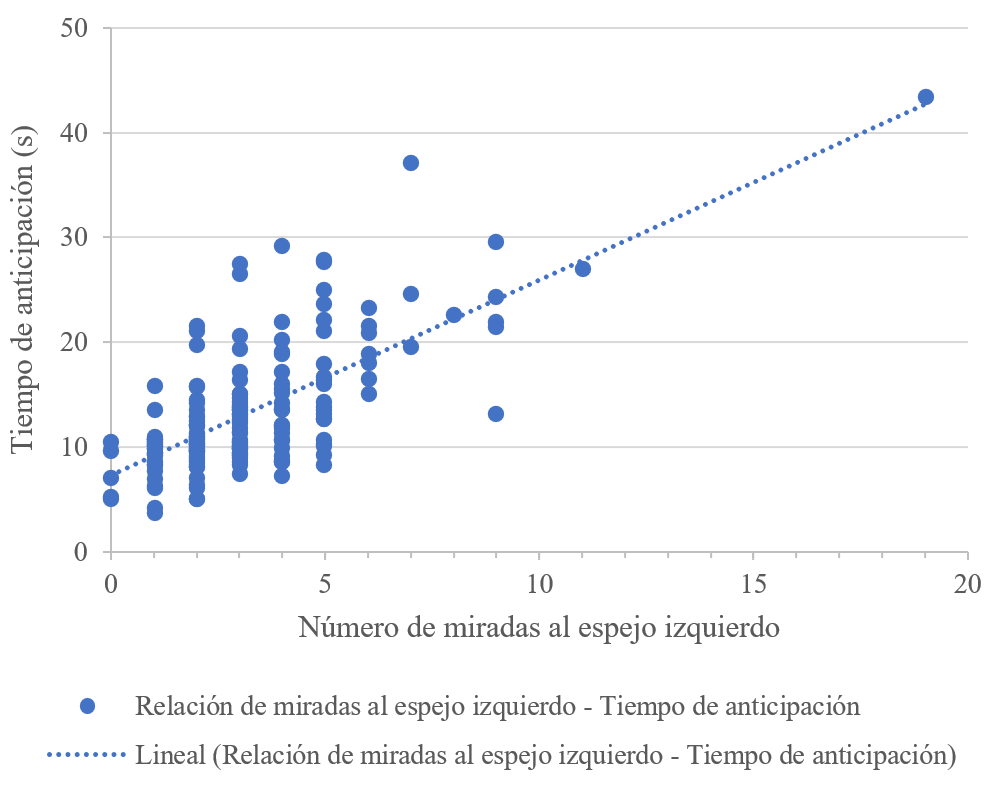
\includegraphics[width=12.5cm]
    {figures/3.15.png}
    \caption{ \label{fig:3.15} Relación de miradas al espejo retrovisor izquierdo con el tiempo de anticipación }
\end{figure}

En las siguientes gráficas se muestra en detalle los resultados obtenidos de toda la muestra para ambas variables (Figura \ref{fig:3.16a} y \ref{fig:3.16b}).

\begin{figure}[h]
  \centering
  \begin{subfigure}[b]{0.45\textwidth}
    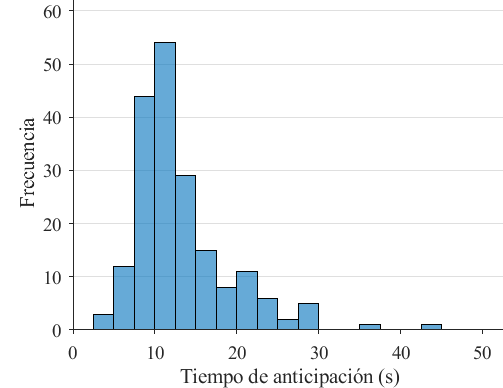
\includegraphics[width=\textwidth]{figures/3.16a.png}
    \caption{}
    \label{fig:3.16a}
  \end{subfigure}
  \hfill
  \begin{subfigure}[b]{0.45\textwidth}
    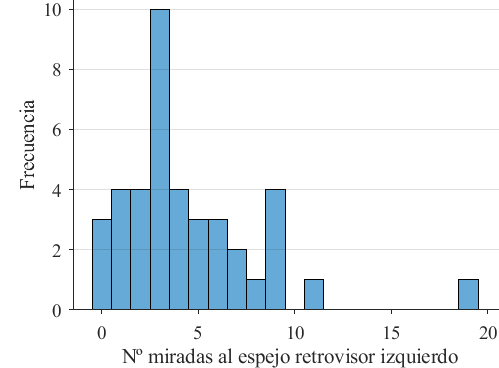
\includegraphics[width=\textwidth]{figures/3.16b.png}
    \caption{}
    \label{fig:3.16b}
  \end{subfigure}
  \caption{(a) Frecuencia del tiempo de anticipación, (b) Frecuencia del número de miradas al espejo retrovisor izquierdo}
  \label{fig:3.16}
\end{figure}

En la figura \ref{fig:3.16a}, se observa que el tiempo de anticipación se produjo en intervalos de entre 4 y 30 segundos antes de cruzar la línea central de la carretera, realizándose a los 10 segundos en la mayoría de los adelantamientos. El número mínimo de miradas para este fenómeno se produjese se determinó en 3, como se observa de forma destacable en la figura \ref{fig:3.16b}. Además, también se pudo advertir que algunos conductores desconectaron la tarea antes de realizar la maniobra, lo que refuerza aún más la indicación de adelantar al vehículo objetivo.
En el análisis de miradas a la tarea se han subdividido dichas etapas, obteniendo cuatro fases diferenciadas en la realización de un adelantamiento: circulación en el carril derecho, \gls{acd}, circulación en el carril izquierdo y \gls{aci} (Figura \ref{fig:3.17}).

\begin{figure}[h]
    \centering
    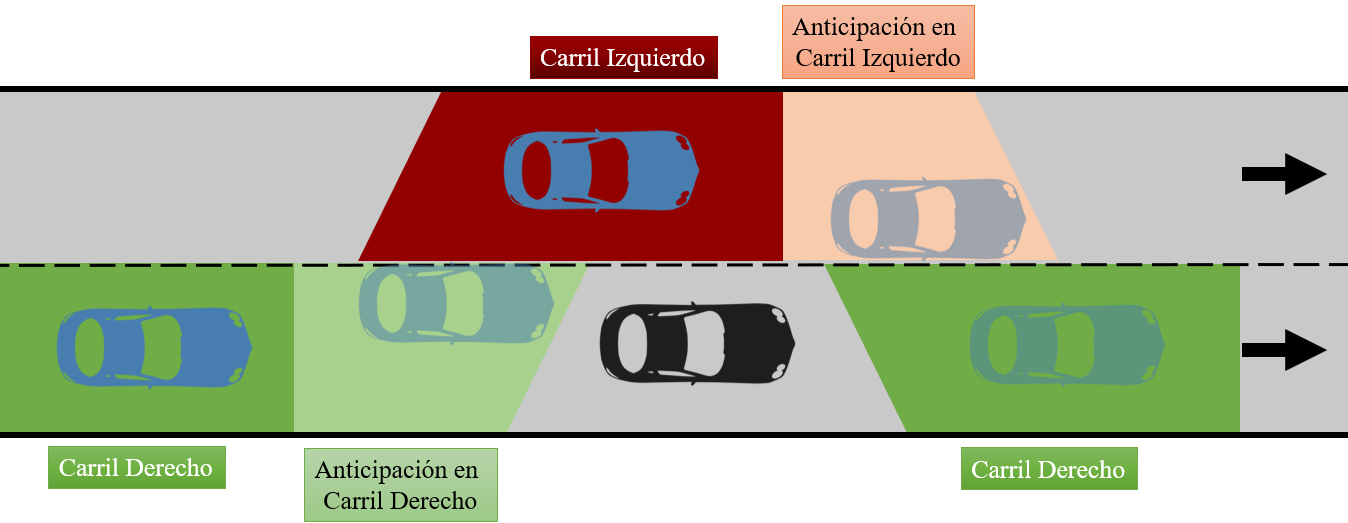
\includegraphics[width=14cm]
    {figures/3.17.png}
    \caption{ \label{fig:3.17} Segmentación de las fases en un cambio de carril}
\end{figure}

\subsection{Metodología }\label{322}

Los participantes del estudio fueron un total de 23 conductores, divididos entre 9 conductores con experiencia previa en el vehículo utilizado y 12 sin experiencia, de los cuales 2 de ellos fueron mujeres. Para el objeto de este estudio solo se han tenido en cuenta los participantes experimentados, siendo todos ellos hombres, elegidos por ser conductores habituales de un vehículo modelo Volvo equipado con el sistema \gls{pa2} de asistencia al pilotaje. También fue requisito el uso de este sistema al menos 3 veces por semana durante un mes. Todos los conductores fueron recompensados con 500SEK (aproximadamente 50€) por su participación en el experimento. La edad de los participantes fue de 47 años (\emph{SD} = 10.74) y la experiencia en conducción de media 29 años (\emph{SD} = 10.74). Dada la naturaleza de este ensayo, es destacable señalar que el protocolo experimental ha respetado el Código Ético de la Asociación Estadounidense de Psicología (\gls{apa}) y fue aprobado por el Comité Regional de Revisión Ética en Linköping, Suecia (DNR: 2016/411- 31).

Los ensayos fueron realizados en una autopista de la ciudad sueca de Linköping en un tramo de 7.5 km de ida y los mismos para la vuelta, siendo su límite de velocidad 110 km/h. Se detectaron un total de 110 adelantamientos, 60 en manual y 50 en modo autónomo, realizando un promedio de 3.05 maniobras por conductor en cada condición y una desviación estándar de 1.47. Durante la conducción, los participantes debían realizar una tarea visuomotora soportada en una tablet ubicada a la derecha del volante. La tarea consistía en una matriz 4 x 4 de flechas apuntado hacia abajo, donde el participante debía señalar si existía algún elemento que apuntase hacia arriba lo más rápido posible mediante los botones \emph{SI} y \emph{NO}, primando siempre la seguridad. Una nueva matriz aparecía cuando el conductor daba una respuesta o después de los 5 segundos si no se registraba nada en el sistema. La tarea disponía de dos modos de funcionamiento: tarea forzosa, la cual demandaba respuestas durante todo el proceso de conducción, y tarea pausable, donde los conductores podían desconectar la tarea mediante un botón sin afectar a su rendimiento, encendiéndola de nuevo en el momento que lo considerasen. En base la puntuación obtenida al finalizar el ensayo, los conductores fueron incentivados lúdicamente con el fin de evitar el exceso de desconexión de la tarea. Para la condición de conducción parcialmente automatizada, se pidió a los conductores que utilizasen el sistema \gls{pa2} en la medida de lo posible, desactivándolo cuando lo considerase necesario. 

El diseño del experimento fue 2 x 2 x 2, con tres variables intrasujeto correspondientes a los niveles de automatización (manuela y autónomo), la pausabilidad de la tarea y la fase del adelantamiento. Todos los participantes realizaron las cuatro condiciones experimentales de manera contrabalanceada para evitar efectos de orden, como la fatiga o el aprendizaje. Las condiciones se resumen en: A) Conducción automatizada + tarea adicional forzosa, B) Conducción automatizada + tarea adicional pausable, C) Conducción manual + tarea adicional forzosa, y D) Conducción manual + tarea adicional pausable. Para las cuatro condiciones solo se eligieron los tramos de adelantamiento que se produjeron dentro de la autopista, y en el último subapartado del estudio, se segmentaron las cuatro fases del adelantamiento definidas anteriormente.

El vehículo utilizado fue un Volvo S90 del 2017 equipado con la segunda versión del sistema de asistencia a la conducción (\gls{pa2}). Dicho sistema combina el funcionamiento de control de crucero adaptativo (\gls{acc}) y el asistente de mantenimiento de carril (\gls{lka}), cuya activación se realiza mediante de los mandos del volante como se indica en la figura \ref{fig:3.18}. El testigo situado bajo el velocímetro indica su estado, presentándose en color verde si el sistema estaba activado en su totalidad o en color gris cuando tenía dificultades para detectar las marcas de carril, funcionando únicamente el \gls{acc}. El vehículo dispone de sensores en el volante que permiten al conductor retirar las manos durante un máximo de 15 segundos cuando el sistema está activado. Si tras ese intervalo no detectase al conductor, el sistema se desconectaría automáticamente por seguridad, indicándolo mediante el testigo visual. 

\newpage
\begin{figure}[h]
    \centering
    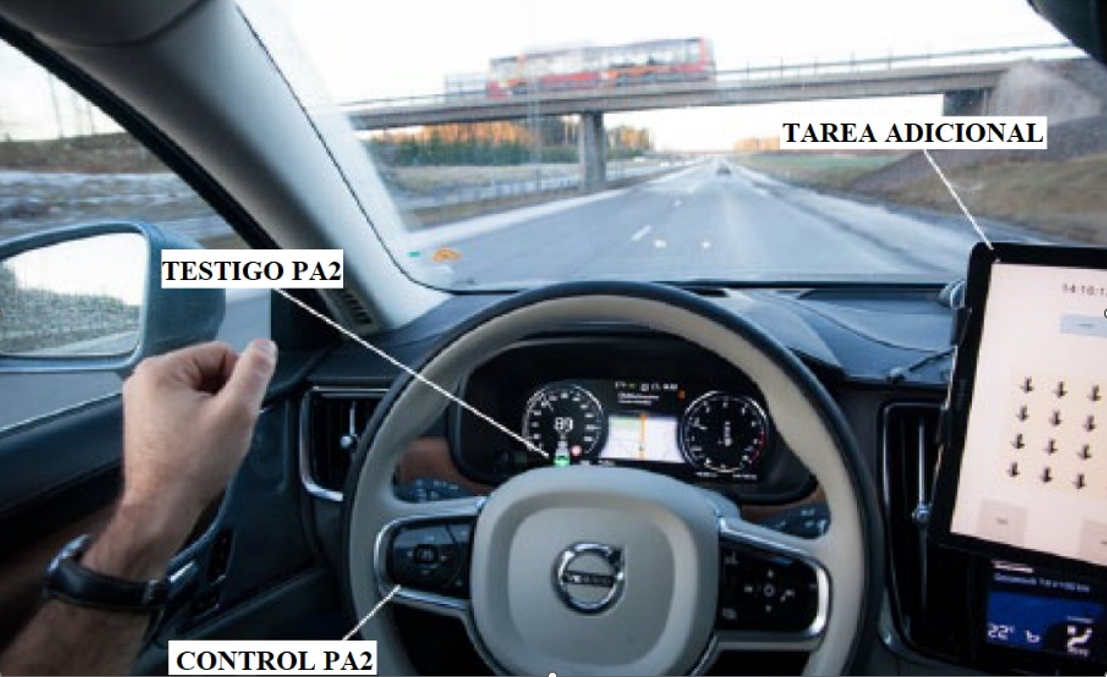
\includegraphics[width=11cm]
    {figures/3.18.png}
    \caption{ \label{fig:3.18} Vista interior vehículo, tarea adicional, símbolo activación del sistema \gls{pa2} (original en \textcite{solismarcos})}
\end{figure}

La adquisición de datos se realizó mediante un par de cámaras que grababan la vista frontal del vehículo y al estado de activación del sistema \gls{pa2}, marca Video VBox Pro. Se utilizó un sistema de posicionamiento global interno (\gls{gps}) para registrar la velocidad, posición y hora, con una frecuencia 10 Hz, y un sistema de seguimiento ocular, marca SMI Eye Tracking Glasses 2.0, para registrar el estado atencional del conductor. Este sistema consiste en unas gafas sensorizadas equipadas con sensores infrarrojos que permiten detectar el comportamiento de la mirada mediante la técnica pupila oscura mencionada anteriormente. Las gafas también disponen de una cámara orientada hacia la escena frontal, que permite la grabación de la mirada del conductor en la carretera. Las variables obtenidas para su procesamiento se observan en la tabla \ref{tab:3.13}.

\begin{table}[h]
\centering
\begin{tabular}{rll}
\textbf{Variables}     & \textbf{Descripción}           & \textbf{Unidades}           \\ \hline
Duración               & Duración del evento observado  & Milisegundos                \\ \hline
Codificación           & Condición del ensayo realizado &                             \\ \hline
Evento                 & Ítem observado                 &                             \\ \hline
Tipo de evento         & Inicio y fin de cada evento    &                             \\ \hline
Video                  & Grabación del ensayo           & 1280 x 960 píxeles a 25 fps \\ \hline
Frecuencia de muestreo &                                & 60 Hz                       \\ \hline
Precisión              &                                & 0.5°                       \\ \hline
\end{tabular}
\caption{Variables del sistema de seguimiento visual SMI Eye Tracking Glasses 2.0}
\label{tab:3.13}
\end{table}

Para el tratamiento de los datos se realizó una fusión del sistema de seguimiento ocular con los videos capturados por las cámaras mediante el software BeGaze Version 3.7. Los eventos fueron codificados manualmente con el software Observer XT Version 13, al igual que las áreas de interés, las cuales fueron panel de mandos, frente, espejo interior, espejo izquierdo, espejo derecho, tarea y otros. El área frente se define como las miradas al carril por el que circula y otros incluye las miradas a los carriles adyacentes, señales y otras zonas del interior del vehículo. Posteriormente se superpusieron los datos adquiridos por la tarea adicional con el resto de los datos para su análisis global.

En cuanto a pruebas estadísticas, se ha aplicado un modelo lineal mixto generalizado utilizando el software Jamovi 2.2.5 con objetivo de analizar la dependencia entre las variables adquiridas por el sistema de seguimiento visual. El ajuste de las comparaciones se realizó mediante el procedimiento de Holm.

\subsection{Resultados}\label{323}

En las condiciones donde la tarea fue pausable, se analizó la probabilidad de que el conductor interrumpiera la tarea durante una maniobra de adelantamiento. Los resultados muestran que solamente el 8.3\% de los conductores pausó la aplicación en conducción parcialmente automatizada, y un 6.2\% en conducción manual, para las condiciones donde la tarea era pausable, B y D respectivamente.

En base a estos resultados, los estudios se han reducido a las condiciones de manual y parcialmente automatizada, ya que no se poseen demasiados datos para la condición de pausabilidad ni se considera que pueda existir ningún efecto significativo, rediseñando el diseño del experimento a 2 x 2 con dos variables intrasujeto y eliminando las incorporaciones donde la tarea estuvo pausada.

\textbf{\emph{Distribución visual durante un adelantamiento}}\label{3231}

La relación de miradas a las diferentes áreas definidas anteriormente ha sido evaluada porcentualmente, observando la variación de pesos a cada objeto a lo largo de la maniobra. Las áreas se definen en panel de mandos, frente, espejo interior, espejo izquierdo, espejo derecho, tarea y otro. La ventana temporal comienza 10 segundos antes del cruce de la línea central, como se explicó anteriormente en el apartado \hyperref[321]{3.2.1.} Definición de un adelantamiento y sus fases, y termina 5 segundos después, a modo informativo sobre la dirección de la mirada tras el cambio de carril. El instante 0 corresponde al evento donde se definió el cruce de la línea que separa los carriles. Las siguientes gráficas representan un adelantamiento de derecha a izquierda (Figura \ref{fig:3.19}) en conducción manual y conducción parcialmente automatizada. 

\begin{figure}[h]
    \centering
    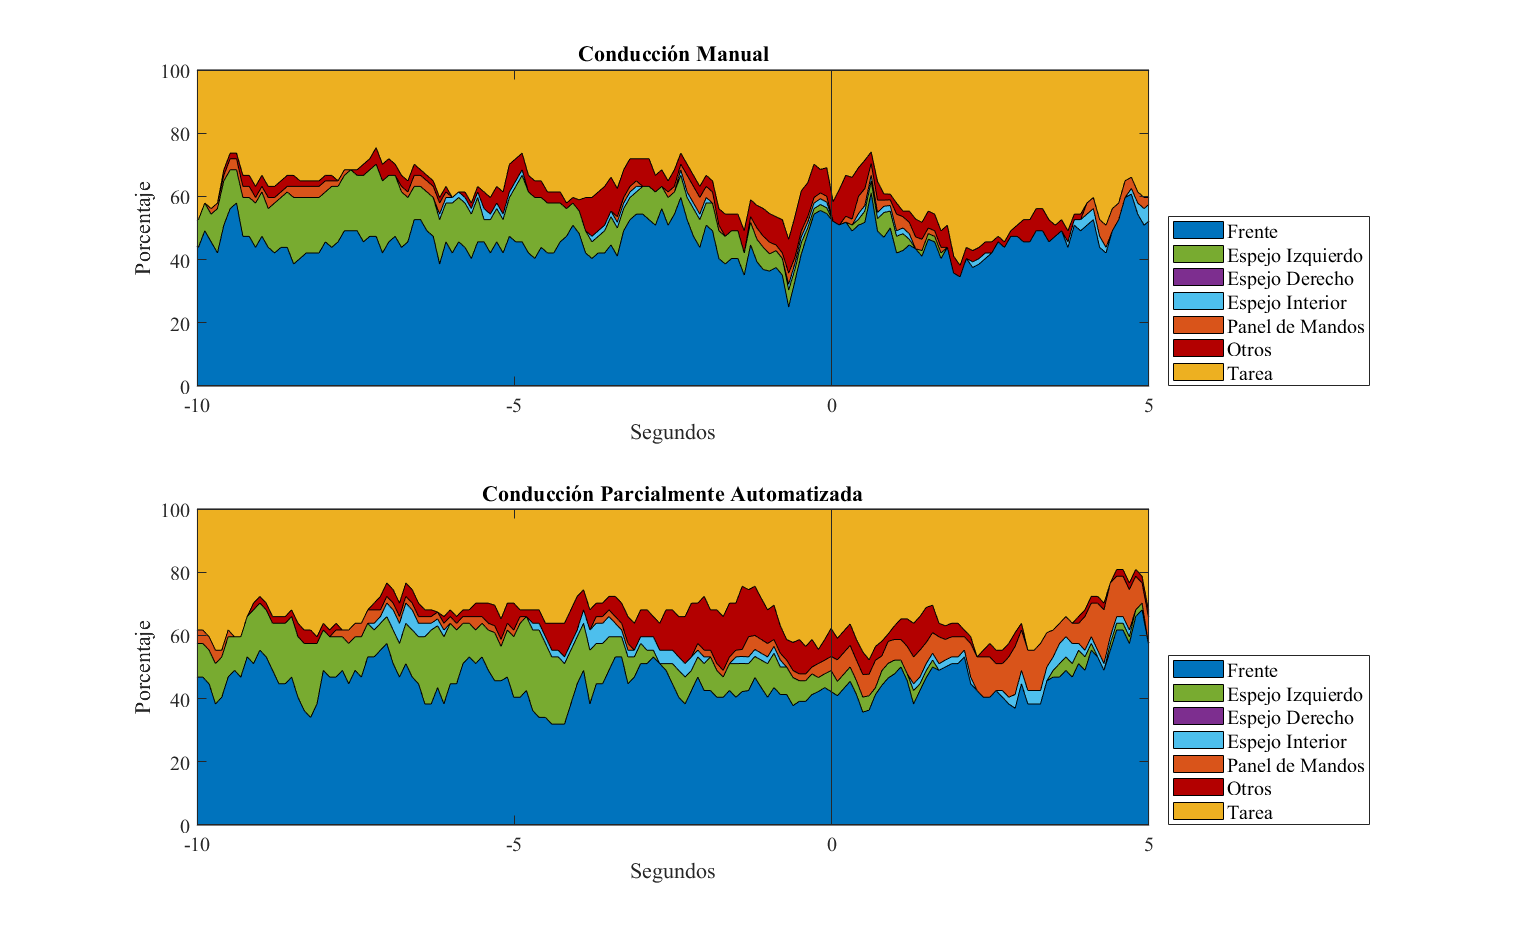
\includegraphics[width=16cm]
    {figures/3.19.png}
    \caption{ \label{fig:3.19} Distribución visual de las miradas durante un adelantamiento en conducción manual y parcialmente automatizada}
\end{figure}

\textbf{\emph{Análisis de la secuencia visual durante un adelantamiento}}\label{3232}

El conjunto de áreas observadas durante un cambio de carril ha sido estudiado analizando la secuencia visual realizada por el conductor. Los resultados se presentan en forma de tabla de probabilidad por parejas contraponiendo las zonas a estudiar para conducción manual y parcialmente automatizada, donde la serie se inicia con el parámetro situado a la izquierda (Entrada) y termina con el parámetro superior (Salida) (Tablas \ref{tab:3.14} y \ref{tab:3.15}). El porcentaje refleja la probabilidad de que se realice una inspección visual desde una entrada y termine en una determinada salida, respecto a la totalidad de las parejas de miradas.

% Please add the following required packages to your document preamble:
% \usepackage[table,xcdraw]{xcolor}
% If you use beamer only pass "xcolor=table" option, i.e. \documentclass[xcolor=table]{beamer}
\begin{table}[h]
\centering
\begin{tabular}{|lccccccc|}
\hline
\multicolumn{8}{|c|}{\textbf{Porcentajes en conducción manual}}                                        \\ \hline
\multicolumn{1}{|l|}{\textit{\begin{tabular}[c]{@{}l@{}}\diagbox[width=9em]{Salida}{Entrada}\end{tabular}}} & \multicolumn{1}{c|}{\textit{\begin{tabular}[c]{@{}c@{}}Panel de \\ mandos\end{tabular}}} & \multicolumn{1}{c|}{\textit{Frente}}               & \multicolumn{1}{c|}{\textit{\begin{tabular}[c]{@{}c@{}}Espejo \\ interior\end{tabular}}} & \multicolumn{1}{c|}{\textit{\begin{tabular}[c]{@{}c@{}}Espejo \\ izquierdo\end{tabular}}} & \multicolumn{1}{c|}{\textit{\begin{tabular}[c]{@{}c@{}}Espejo \\ derecho\end{tabular}}} & \multicolumn{1}{c|}{\textit{Tarea}}                & \textit{Otros}               \\ \hline
\multicolumn{1}{|l|}{\textit{Panel de mandos}}                                                & \multicolumn{1}{c|}{\cellcolor[HTML]{C9C9C9}}                                            & \multicolumn{1}{c|}{\cellcolor[HTML]{EFF5FC}2.62}  & \multicolumn{1}{c|}{\cellcolor[HTML]{FCFCFF}0}                                           & \multicolumn{1}{c|}{\cellcolor[HTML]{FCFCFF}0}                                            & \multicolumn{1}{c|}{\cellcolor[HTML]{FCFCFF}0}                                          & \multicolumn{1}{c|}{\cellcolor[HTML]{FBFCFF}0.26}  & \cellcolor[HTML]{FCFCFF}0.09 \\ \hline
\multicolumn{1}{|l|}{\textit{Frente}}                                                         & \multicolumn{1}{c|}{\cellcolor[HTML]{EFF4FC}2.71}                                        & \multicolumn{1}{c|}{\cellcolor[HTML]{C9C9C9}}      & \multicolumn{1}{c|}{\cellcolor[HTML]{F3F7FD}1.92}                                        & \multicolumn{1}{c|}{\cellcolor[HTML]{D6E5F5}7.70}                                         & \multicolumn{1}{c|}{\cellcolor[HTML]{FAFBFF}0.44}                                       & \multicolumn{1}{c|}{\cellcolor[HTML]{5F9ED7}31.50} & \cellcolor[HTML]{EFF4FC}2.71 \\ \hline
\multicolumn{1}{|l|}{\textit{Espejo interior}}                                                & \multicolumn{1}{c|}{\cellcolor[HTML]{FCFCFF}0}                                           & \multicolumn{1}{c|}{\cellcolor[HTML]{F6F8FE}1.40}  & \multicolumn{1}{c|}{\cellcolor[HTML]{C9C9C9}}                                            & \multicolumn{1}{c|}{\cellcolor[HTML]{FCFCFF}0}                                            & \multicolumn{1}{c|}{\cellcolor[HTML]{FCFCFF}0.09}                                       & \multicolumn{1}{c|}{\cellcolor[HTML]{F9FAFF}0.70}  & \cellcolor[HTML]{FCFCFF}0    \\ \hline
\multicolumn{1}{|l|}{\textit{Espejo izquierdo}}                                               & \multicolumn{1}{c|}{\cellcolor[HTML]{FCFCFF}0}                                           & \multicolumn{1}{c|}{\cellcolor[HTML]{D5E5F5}7.87}  & \multicolumn{1}{c|}{\cellcolor[HTML]{FCFCFF}0}                                           & \multicolumn{1}{c|}{\cellcolor[HTML]{C9C9C9}}                                             & \multicolumn{1}{c|}{\cellcolor[HTML]{FCFCFF}0}                                          & \multicolumn{1}{c|}{\cellcolor[HTML]{F7F9FE}1.14}  & \cellcolor[HTML]{FCFCFF}0.17 \\ \hline
\multicolumn{1}{|l|}{\textit{Espejo derecho}}                                                 & \multicolumn{1}{c|}{\cellcolor[HTML]{FCFCFF}0}                                           & \multicolumn{1}{c|}{\cellcolor[HTML]{FCFCFF}0.17}  & \multicolumn{1}{c|}{\cellcolor[HTML]{FCFCFF}0}                                           & \multicolumn{1}{c|}{\cellcolor[HTML]{FCFCFF}0}                                            & \multicolumn{1}{c|}{\cellcolor[HTML]{C9C9C9}}                                           & \multicolumn{1}{c|}{\cellcolor[HTML]{FCFCFF}0.17}  & \cellcolor[HTML]{FCFCFF}0    \\ \hline
\multicolumn{1}{|l|}{\textit{Tarea}}                                                          & \multicolumn{1}{c|}{\cellcolor[HTML]{FCFCFF}0.17}                                        & \multicolumn{1}{c|}{\cellcolor[HTML]{5B9BD5}32.28} & \multicolumn{1}{c|}{\cellcolor[HTML]{FCFCFF}0.17}                                        & \multicolumn{1}{c|}{\cellcolor[HTML]{FBFCFF}0.26}                                         & \multicolumn{1}{c|}{\cellcolor[HTML]{FCFCFF}0}                                          & \multicolumn{1}{c|}{\cellcolor[HTML]{C9C9C9}}      & \cellcolor[HTML]{F7F9FE}1.14 \\ \hline
\multicolumn{1}{|l|}{\textit{Otros}}                                                          & \multicolumn{1}{c|}{\cellcolor[HTML]{FCFCFF}0.09}                                        & \multicolumn{1}{c|}{\cellcolor[HTML]{F0F5FC}2.54}  & \multicolumn{1}{c|}{\cellcolor[HTML]{FCFCFF}0.09}                                        & \multicolumn{1}{c|}{\cellcolor[HTML]{FBFCFF}0.26}                                         & \multicolumn{1}{c|}{\cellcolor[HTML]{FCFCFF}0}                                          & \multicolumn{1}{c|}{\cellcolor[HTML]{F6F9FE}1.31}  & \cellcolor[HTML]{C9C9C9}     \\ \hline
\end{tabular}
\caption{Secuencias visuales durante un adelantamiento en conducción manual}
\label{tab:3.14}
\end{table}

% Please add the following required packages to your document preamble:
% \usepackage[table,xcdraw]{xcolor}
% If you use beamer only pass "xcolor=table" option, i.e. \documentclass[xcolor=table]{beamer}
\begin{table}[h]
\centering
\begin{tabular}{|llllllll|}
\hline
\multicolumn{8}{|c|}{\textbf{Porcentajes en conducción parcialmente automatizada}} 
\\ \hline
\multicolumn{1}{|l|}{\textit{\begin{tabular}[c]{@{}l@{}}\diagbox[width=9em]{Salida}{Entrada}\end{tabular}}} & \multicolumn{1}{c|}{\textit{\begin{tabular}[c]{@{}c@{}}Panel de \\ mandos\end{tabular}}} & \multicolumn{1}{c|}{\textit{Frente}}               & \multicolumn{1}{c|}{\textit{\begin{tabular}[c]{@{}c@{}}Espejo \\ interior\end{tabular}}} & \multicolumn{1}{c|}{\textit{\begin{tabular}[c]{@{}c@{}}Espejo \\ izquierdo\end{tabular}}} & \multicolumn{1}{c|}{\textit{\begin{tabular}[c]{@{}c@{}}Espejo \\ derecho\end{tabular}}} & \multicolumn{1}{c|}{\textit{Tarea}}                & \multicolumn{1}{c|}{\textit{Otros}} \\ \hline
\multicolumn{1}{|l|}{\textit{Panel de mandos}}                                                & \multicolumn{1}{l|}{\cellcolor[HTML]{C9C9C9}}                                            & \multicolumn{1}{l|}{\cellcolor[HTML]{D9E7F6}5.95}  & \multicolumn{1}{l|}{\cellcolor[HTML]{FCFCFF}0}                                           & \multicolumn{1}{l|}{\cellcolor[HTML]{FCFCFF}0}                                            & \multicolumn{1}{l|}{\cellcolor[HTML]{FCFCFF}0}                                          & \multicolumn{1}{l|}{\cellcolor[HTML]{F7F9FE}0.86}  & \cellcolor[HTML]{FBFCFF}0.22        \\ \hline
\multicolumn{1}{|l|}{\textit{Frente}}                                                         & \multicolumn{1}{l|}{\cellcolor[HTML]{D7E6F6}6.16}                                        & \multicolumn{1}{l|}{\cellcolor[HTML]{C9C9C9}}      & \multicolumn{1}{l|}{\cellcolor[HTML]{F4F7FD}1.41}                                        & \multicolumn{1}{l|}{\cellcolor[HTML]{C4DAF1}9.41}                                         & \multicolumn{1}{l|}{\cellcolor[HTML]{FCFCFF}0}                                          & \multicolumn{1}{l|}{\cellcolor[HTML]{619FD7}25.73} & \cellcolor[HTML]{EAF1FB}3.14        \\ \hline
\multicolumn{1}{|l|}{\textit{Espejo interior}}                                                & \multicolumn{1}{l|}{\cellcolor[HTML]{FCFCFF}0}                                           & \multicolumn{1}{l|}{\cellcolor[HTML]{F5F8FE}1.19}  & \multicolumn{1}{l|}{\cellcolor[HTML]{C9C9C9}}                                            & \multicolumn{1}{l|}{\cellcolor[HTML]{FCFCFF}0}                                            & \multicolumn{1}{l|}{\cellcolor[HTML]{FBFCFF}0.22}                                       & \multicolumn{1}{l|}{\cellcolor[HTML]{FBFBFF}0.32}  & \cellcolor[HTML]{FCFCFF}0           \\ \hline
\multicolumn{1}{|l|}{\textit{Espejo izquierdo}}                                               & \multicolumn{1}{l|}{\cellcolor[HTML]{FCFCFF}0}                                           & \multicolumn{1}{l|}{\cellcolor[HTML]{C1D9F0}9.84}  & \multicolumn{1}{l|}{\cellcolor[HTML]{FCFCFF}0}                                           & \multicolumn{1}{l|}{\cellcolor[HTML]{C9C9C9}}                                             & \multicolumn{1}{l|}{\cellcolor[HTML]{FCFCFF}0}                                          & \multicolumn{1}{l|}{\cellcolor[HTML]{F9FAFE}0.65}  & \cellcolor[HTML]{FBFCFF}0.22        \\ \hline
\multicolumn{1}{|l|}{\textit{Espejo derecho}}                                                 & \multicolumn{1}{l|}{\cellcolor[HTML]{FCFCFF}0}                                           & \multicolumn{1}{l|}{\cellcolor[HTML]{FCFCFF}0.11}  & \multicolumn{1}{l|}{\cellcolor[HTML]{FCFCFF}0}                                           & \multicolumn{1}{l|}{\cellcolor[HTML]{FCFCFF}0}                                            & \multicolumn{1}{l|}{\cellcolor[HTML]{C9C9C9}}                                           & \multicolumn{1}{l|}{\cellcolor[HTML]{FCFCFF}0.11}  & \cellcolor[HTML]{FCFCFF}0           \\ \hline
\multicolumn{1}{|l|}{\textit{Tarea}}                                                          & \multicolumn{1}{l|}{\cellcolor[HTML]{F9FAFE}0.65}                                        & \multicolumn{1}{l|}{\cellcolor[HTML]{5B9BD5}26.70} & \multicolumn{1}{l|}{\cellcolor[HTML]{FBFBFF}0.32}                                        & \multicolumn{1}{l|}{\cellcolor[HTML]{FBFBFF}0.32}                                         & \multicolumn{1}{l|}{\cellcolor[HTML]{FCFCFF}0}                                          & \multicolumn{1}{l|}{\cellcolor[HTML]{C9C9C9}}      & \cellcolor[HTML]{F4F7FD}1.41        \\ \hline
\multicolumn{1}{|l|}{\textit{Otros}}                                                          & \multicolumn{1}{l|}{\cellcolor[HTML]{FBFBFF}0.32}                                        & \multicolumn{1}{l|}{\cellcolor[HTML]{ECF3FB}2.70}  & \multicolumn{1}{l|}{\cellcolor[HTML]{FBFCFF}0.22}                                        & \multicolumn{1}{l|}{\cellcolor[HTML]{FBFCFF}0.22}                                         & \multicolumn{1}{l|}{\cellcolor[HTML]{FCFCFF}0}                                          & \multicolumn{1}{l|}{\cellcolor[HTML]{F3F7FD}1.62}  & \cellcolor[HTML]{C9C9C9}            \\ \hline
\end{tabular}
\caption{Secuencias visuales durante un adelantamiento en conducción parcialmente automatizada}
\label{tab:3.15}
\end{table}

Los colores representan las relaciones más frecuentes y la intensidad los valores más altos. Los valores obtenidos representan de manera numérica los resultados del apartado anterior \emph{Distribución visual durante un adelantamiento}. 

\textbf{\emph{Miradas a la tarea secundaria según fases de un adelantamiento}}\label{3233}

Las relaciones de los parámetros obtenidos del sistema de seguimiento visual, duración media de miradas y número de miradas por segundo a la tarea, han sido estudiadas mediante un modelo lineal mixto generalizado. Dado que el nivel de pausabilidad de la tarea no se ha considerado relevante, debido a la escasa cantidad de datos, el modelo queda reducido a los niveles de automatización y fase. Se observaron efectos principales en la duración media de miradas a la tarea en la condición automatización (\emph{F} (1;109) = 7.85, \emph{p} = 0.006) y en fase (\emph{F} (1;109) = 11.94, \emph{p} < 0.001), al igual que para el número de miradas por segundo a la tarea en la condición automatización (\emph{F} (1;107) = 10.78, \emph{p} = 0.001) y en fase (\emph{F} (1;107) = 4.19, \emph{p} = 0.008).
Estos efectos pueden verse en la figura \ref{fig:3.20} y figura \ref{fig:3.21} para ambas variables, a través de la representación de las medias en cada modo de automatización por fases.  

\begin{figure}[h]
    \centering
    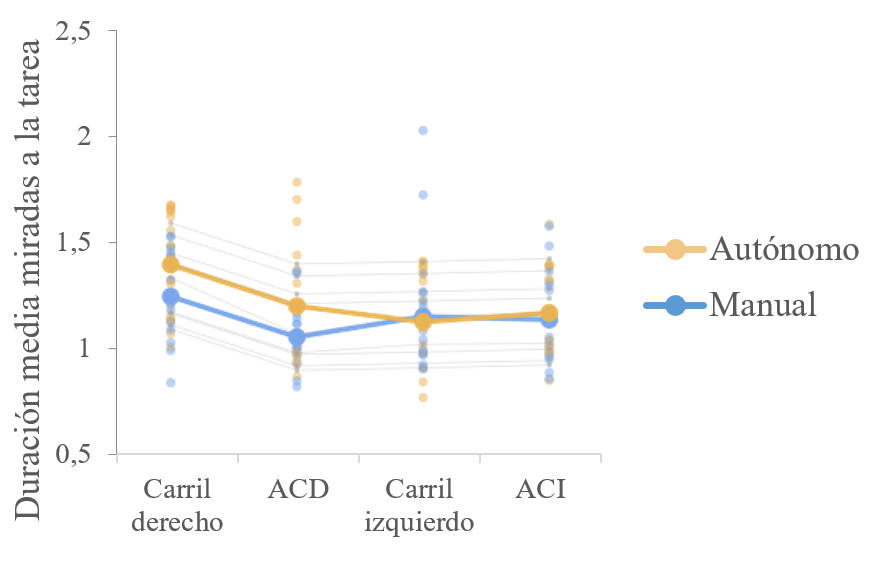
\includegraphics[width=10.5cm]
    {figures/3.20.png}
    \caption{ \label{fig:3.20} Efectos en duración media de miradas a la tarea en cada modo de automatización por fases del adelantamiento}
\end{figure}

\begin{figure}[h]
    \centering
    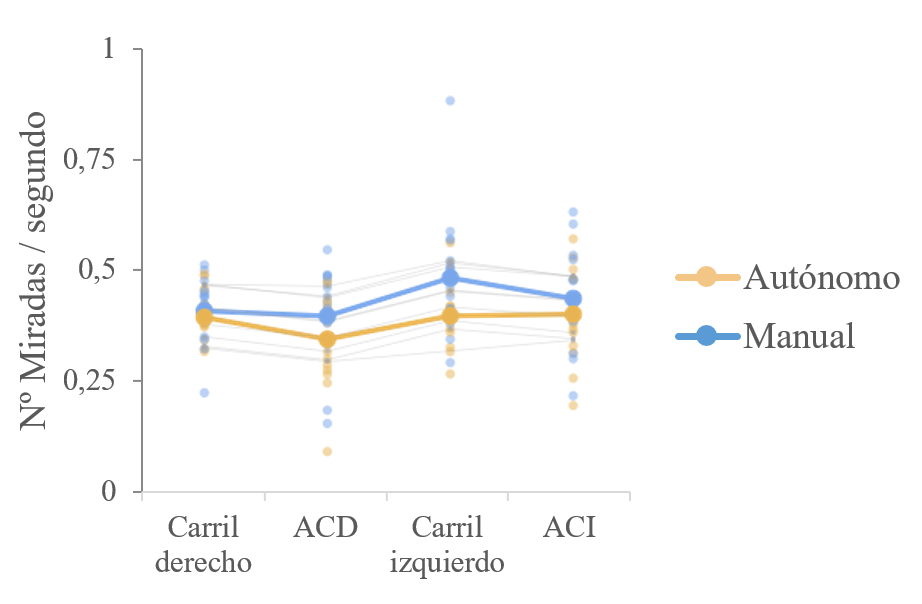
\includegraphics[width=10.5cm]
    {figures/3.21.png}
    \caption{ \label{fig:3.21} Efectos en número de miradas por segundo a la tarea en cada modo de automatización por fases del adelantamiento}
\end{figure}

Se puede apreciar que en duración media existe un efecto en carril derecho y en \gls{acd}, destacando que todos los datos los valores para autónomo son mayores que manual. Por el contrario, el número de fijaciones fueron mayores en manual que en autónomo, donde el efecto aparece en la zona de carril izquierdo. Los efectos aleatorios se muestran al fondo en línea fina. 

Para valorar si el efecto es significativo, en la tabla \ref{tab:3.16} se recogen los valores p de cada zona en función del nivel de automatización.

\begin{table}[h]
\centering
\begin{tabular}{rccl}
\textbf{}                                                                      & \multicolumn{3}{c}{\textbf{Valor \emph{p} entre modos de automatización}}                                                                                                                     \\ \hline
\textbf{Fases del adelantamiento}                                              & \begin{tabular}[c]{@{}c@{}}Duración media \\ miradas a la tarea\end{tabular} & \multicolumn{2}{c}{\begin{tabular}[c]{@{}c@{}}N.$^\circ$ miradas /segundo \\ a la tarea\end{tabular}} \\ \hline
Carril derecho                                                                 & 0.100                                                                                 & \multicolumn{2}{c}{1.000}                                                                      \\ \hline
\begin{tabular}[c]{@{}r@{}}Anticipación \\ Carril Derecho (\gls{acd})\end{tabular}   & 0.166                                                                                 & \multicolumn{2}{c}{1.000}                                                                      \\ \hline
Carril izquierdo                                                               & 1.000                                                                                 & \multicolumn{2}{c}{0.088}                                                                      \\ \hline
\begin{tabular}[c]{@{}r@{}}Anticipación \\ Carril izquierdo (\gls{aci})\end{tabular} & 1.000                                                                                 & \multicolumn{2}{c}{1.000}                                                                      \\ \hline
\end{tabular}
\caption{Valores p para las variables de seguimiento visual en automatización y fases del adelantamiento}
\label{tab:3.16}
\end{table}

Los datos obtenidos del modelo denotan no existe ningún efecto significativo en ninguna de las dos variables tras la corrección de Holm en el valor \emph{p}. No obstante, se pueden apreciar ciertas tendencias a través de las gráficas y los resultados expuestos.

\subsection{Discusión}\label{324}

La maniobra del cambio de carril ha sido analizada en las condiciones de conducción manual y parcialmente automatizada, mientras se realizaba una tarea secundaria durante la conducción. A pesar de que la tarea era pausable, pocos conductores consideraron realizar interrupciones a la misma, observándose este hecho tanto en manual como en parcialmente automatizado. No obstante, la razón de estos resultados puede explicarse por el uso habitual de dispositivos móviles, ya que los conductores han aprendido a gestionar la atención entre la conducción y el uso del mismo de manera segura. 

En la distribución visual se han advertido diferentes modos de gestionar los recursos cognitivos durante un adelantamiento en función del tipo de conducción. El resultado más notable es la evolución de las miradas al espejo izquierdo (color verde), dado que el adelantamiento es hacia la izquierda y se producía de manera manual en ambos casos. Las miradas al espejo izquierdo entre los segundos 5 y 10 previos al cambio de carril conforman un 20\% de las miradas totales en esa zona, ya que corresponden a la fase de anticipación, adquisición y gestión de la información para realizar la maniobra. Los siguientes 5 segundos pueden considerarse de ejecución, dado el descenso de miradas al espejo izquierdo y el aumento a otras áreas como tarea, frente y otros. 

A grandes rasgos se puede decir que el valor medio de las miradas en ambos casos es muy similar y que la principal diferencia es la forma de la curva. En relación con las diferencias entre conducción manual y parcialmente automatizada, se observa que las miradas al frente en manual son bastante constantes en todo el periodo de anticipación, mientras que en automatizado se pueden percibir hasta tres valles con variaciones de aproximadamente un 10-15\%. Esta disminución es debida a la activación del sistema, que, al liberar al conductor del proceso de seguir al vehículo de delante, puede derivar su atención a otras áreas que lo requieran. Estos hechos ocurren de manera contraria con las miradas a la tarea. En automatizado se puede apreciar que la atención a la tarea oscila entre 30-40\% de las miradas totales, pero en manual los valores llegan a un 50\%, notando dos repuntes (si se viera la figura girada) entre los segundos 3 y 7 previos al adelantamiento. En base a estos resultados, se puede deducir que en conducción manual se priorizan las miradas al frente ante la tarea secundaria, y a la inversa en conducción parcialmente automatizada.

Por último, se puede observar notablemente que en la condición automatizado hay más miradas a otros factores de la vía, e incluso al espejo interior. El instante donde se rebasa la línea también difiere en ambos modos de funcionamiento, ya que en conducción manual las miradas al frente son un 20\% mayores que en parcialmente automatizada. El área del panel de mandos recobra importancia al terminar la maniobra en conducción parcialmente automatizada, ya que el conductor dirige su atención para comprobar que el sistema \gls{pa2} está nuevamente activado durante la circulación en el carril izquierdo.

En relación con la secuencia visual, se estudió a través de una tabla de probabilidad para ambas condiciones. Globalmente se puede distinguir que las relaciones más fuertes son simétricas respecto a la diagonal, donde las variables más observadas son al frente, a la tarea, al espejo izquierdo y al panel de mandos, independientemente de cuál sea el primer parámetro.  Este resultado confirma el sesgo de fijación central para la zona frente. Comparativamente las relaciones entre tarea y frente fueron superiores en manual, reforzando la conclusión del apartado anterior sobre la influencia del sistema \gls{pa2} en la gestión atencional. Sin embargo, en la condición automatizado fueron superiores las relaciones frente con espejo izquierdo y panel de mandos, debido a que las salidas al frente fueron inferiores en todos los demás parámetros. Este resultado se relaciona con el aumento de miradas a otros factores, fruto de la conducción autónoma observado también en el apartado anterior.

En el último apartado, se analizaron las variables atencionales a la tarea secundaria obteniendo efectos principales en los niveles de automatización y fase del adelantamiento. Sin embargo, tras evaluar en detalle los resultados, se concluyó que ninguno de los efectos observados era significativo. 

Analizando los resultados en detalle se observa que, tal y como se defendía en el apartado anterior, la conducción parcialmente automatizada permite al conductor derivar su atención a otras áreas, dando sentido a una duración media de la mirada a la tarea levemente superior en el modo autónomo. Este valor es especialmente mayor en las fases del carril derecho y \gls{acd}, debido a que en estos periodos el sistema \gls{pa2} continuaba activado hasta que el conductor decidió adelantar. Las siguientes fases en el carril izquierdo son bastante similares entre sí en ambos modos de funcionamiento. Es destacable la pendiente negativa que se observa en la duración media de las miradas en modo autónomo entre fases, ya que la complejidad de la maniobra no permite al conductor dedicar el tiempo necesario a la ejecución de la tarea.

Ocurre lo contrario en el número de miradas por segundo a la tarea, donde los valores en manual fueron levemente superiores en la condición de autónoma. Un aumento en esta variable es un posible indicador de una mayor carga cognitiva, ya que el conductor debe volver a mirar la escena al no conseguir extraer la información suficiente. En el carril izquierdo se puede apreciar un incremento notable respecto a las demás fases en ambos modos de funcionamiento que, junto a los valores de duración media de las miradas, remarcan esta zona como la más demandante del cambio de carril seguida de la fase \gls{aci}.

\section{Conclusiones}\label{33}

La atención visual de un conductor es un parámetro muy interesante para la evaluación de estrategias atencionales que puedan ser aplicadas a la mejora de algoritmos de toma de decisiones en conducción autónoma. El análisis de la carga cognitiva, la atención visual y la gestión atencional del conductor mediante un sistema de seguimiento visual, ha permitido extraer conclusiones sobre su estado cognitivo frente a maniobras complejas, como incorporación a una vía principal o cambio de carril. 

Las incorporaciones en autovías son situaciones muy demandantes donde la experiencia y la edad influyen decisivamente en la carga mental. Analizando la maniobra se desarrolló una aplicación de ayuda a la incorporación, la cual obtuvo resultados satisfactorios entre los conductores. La localización fue determinada gracias a la obtención de mapas de calor de las miradas durante la maniobra, hallando un punto caliente en la esquina interior-superior del espejo retrovisor. Esta zona permite extraer suficiente información de la escena a través de la visión periférica, observando el espejo retrovisor pero sin dejar de atender al frente. El diseño de la interfaz fue validado en los aspectos satisfacción, utilidad y usabilidad, donde se encontraron relaciones directas con las variables atencionales del conductor. La satisfacción que tiene un conductor sobre un sistema está conectada con la usabilidad que percibe del mismo y la exigencia mental, al igual que la utilidad que concibe de un \gls{adas} con el número de miradas y el seguimiento visual. Este hecho pone el foco de atención en la importancia del diseño de los sistemas de asistencia, ya que si el conductor no percibe su uso positivamente será descartado afectando directamente la seguridad del vehículo. 

Respecto a los adelantamientos, se estudió la gestión atencional en conducción manual y parcialmente automatizada durante la maniobra, mientras se realizaba una tarea secundaria en una autovía en tráfico real. Los resultados obtenidos mostraron que los conductores, a pesar de tener la posibilidad de pausar la tarea durante la maniobra, realizaron pocas interrupciones en ambos modos de funcionamiento, posiblemente debido a que no consideraron la tarea como distractora y a la transferencia de conocimiento en el uso de teléfonos móviles y pantallas de navegación durante la conducción. Se considera que un intervalo de 10 segundos es suficiente para analizar el periodo de anticipación durante un adelantamiento, en base a estrategias comunes a todas las muestras. La distribución y secuencias visuales mostraron información similar, aportando que las áreas más observadas fueron al frente o carril central y la tarea, con diferencias entre la conducción manual y parcialmente automatizada pero siempre priorizando la seguridad en ambos casos. El sistema \gls{pa2} permitió al conductor liberarse de supervisar la zona de frente para poder explorar otras áreas del entorno además de dedicar más atención a la tarea. En el análisis por zonas durante la maniobra de adelantamiento se percibió que la zona de carril izquierdo fue la fase más demandante cognitivamente en conducción manual, al contrario que las fases de carril derecho y anticipación al cambio de carril desde la derecha, donde el sistema \gls{pa2} estuvo activado en conducción parcialmente automatizada.

El comportamiento y las intenciones de un conductor pueden reflejar las estrategias internas en la toma de decisiones, siendo dicha información interesante en la caracterización de respuestas ante diversos escenarios en conducción autónoma. Sin embargo, es habitual que la identificación de áreas de interés se codifique de forma manual a través de imágenes y vídeos, dando como resultado una tarea tediosa e inexacta.

En los siguientes capítulos se realizará una integración de las variables de la mirada con los demás sensores de detección del entorno, con objeto de automatizar el proceso de identificación de áreas de interés en sistemas de seguimiento visual. Posteriormente se estudiará la influencia de las mismas en la toma de decisiones que realiza el conductor, permitiendo el desarrollo de algoritmos más naturalistas que ayuden a la integración de los vehículos autónomos en el tráfico mixto.


\makechapter{Fusión sensorial}{Fusión sensorial}{Fusión sensorial}\label{ch4}
Correlacionar la mirada del conductor en el espacio resulta de gran interés, ya que permite desarrollar herramientas que integren nuevas variables atencionales en los algoritmos de toma de decisiones, otorgándoles un mayor nivel de naturalismo. Sin embargo, se encuentran pocos estudios donde se desarrolle una fusión de la mirada del conductor con los elementos del entorno de forma automática. Algunos programas sofisticados están trabajando en soluciones basadas en inteligencia artificial, como es el ejemplo de SmartEye, que permite la identificación de la atención del usuario a la vez que la determinación de la naturaleza del objeto mirado. Pero la realidad es que muchos ensayos de seguimiento visual se siguen procesando de manera manual, realizando codificaciones en las imágenes o vídeos sobre el tipo de evento observado, cuya tarea puede ser bastante tediosa e inexacta en función de la duración del ensayo.

La integración de la mirada del conductor hacia el exterior del vehículo requiere de un paso intermedio que permita referenciar todos los sistemas en un origen de coordenadas común. La clave de esta cuestión reside en la determinación del movimiento de la cabeza, ya que sirve para referenciar el campo de visión del conductor en el espacio. Esta solución se encuentra en algunos estudios de la literatura como en \textcite{deng}, donde se integró el movimiento de la cabeza a través de una cámara que localizaba la posición facial del conductor. Este sistema permitió determinar la dirección de la mirada a los objetos durante un cambio de carril en un entorno de simulación. En \textcite{langner} se realizaron experimentos en conducción real sobre la conciencia situacional en el tráfico, fusionando el sistema de seguimiento visual del conductor con imágenes del exterior, captadas por unas cámaras estéreo instaladas en el vehículo. Esta integración fue posible mediante un sistema basado en LEDs infrarrojos y marcadores fiduciales para determinar el movimiento de la cabeza.

Como se observó en el capítulo anterior, la mirada del conductor es una variable muy importante para comprender su estado y sus intenciones frente a los diferentes eventos. Dado el campo visual del conductor es móvil respecto al entorno, en los siguientes apartados se desarrollará un sistema basado en cámaras y sensores infrarrojos para fusionar la dirección de la mirada con los obstáculos del entorno a través del movimiento de la cabeza. Los sistemas de percepción utilizados son descritos en los siguientes apartados, así como especificaciones, precisión e integración de los mismos. Para la mirada del conductor se ha empleado un sistema de seguimiento visual poco intrusivo utilizado en el anterior capitulo. 

\section{Sistemas de percepción}\label{41}

\subsection{Percepción del entorno y vehículo}\label{411}

Una de las claves en la conducción, ya sea autónoma o manual, es el conocimiento de los obstáculos que conforman el medio por el que se mueve el vehículo. Dicha tarea no siempre es sencilla ante condiciones de baja visibilidad, ángulos muertos, oscuridad, inclemencias meteorológicas o modificaciones temporales en las infraestructuras. En la actualidad, la mayoría de los vehículos se comercializan equipados con algún sensor de detección del entorno, estando presente desde los niveles más bajos de automatización, donde cobran protagonismo los sistemas de asistencia al conductor (\gls{adas}), hasta los niveles más altos, donde no se precisa de la supervisión del conductor para realizar un trayecto. 

La información proporcionada por los sensores y su correcta interpretación, suponen la base sobre la que trabajan muchos algoritmos de control, por lo que se requiere un rendimiento alto y fiable (\cite{yeong}).Es por ello que, en numerosas ocasiones, se pueden encontrar estudios (\cite{kim}; \cite{li21b}) donde se busca la redundancia entre sensores para enriquecer una investigación y dotar de robustez la seguridad de los sistemas, mejorando la detección de falsos positivos y la pérdida de datos. La fusión sensorial se basa en la detección simultánea de un objeto captada por más de un sensor, pudiendo ser del mismo tipo (\cite{fan}; \cite{kemsaram}) o de naturalezas diferentes (\cite{gehrig}; \cite{caesar}). Los sensores de detección más comunes en automoción son cámaras, sistemas láser y radar. 

En el presente capítulo se realiza una fusión sensorial sencilla entre el sistema de seguimiento visual utilizado en el capítulo anterior y los sensores de percepción del entorno equipados en el vehículo, los cuales consisten en una cámara de visión artificial y un sensor láser descritos en el apartado \hyperref[42]{4.2 Instrumentación y procesamiento de datos}. Estos dos sistemas de percepción se encuentran muy extendidos en el mundo de la automoción por sus ventajas frente a otros sensores en cuanto a capacidad de detección y facilidad de análisis de los datos, y son complementarios en la generación de mapas de profundidad (\cite{berrio}; \cite{mendez}; \cite{bai}).

\subsection{Percepción del conductor}\label{412}

Es un hecho que los eventos del entorno influencian directamente en las intenciones y los actos de un conductor. Una herramienta muy utilizada para evaluar la atención en conducción y explorar las estrategias visuales del conductor es el seguimiento visual, estando cada vez más extendida en el campo de la conducción automatizada (\cite{liang}; \cite{solismarcos}). Uno de los mayores desafíos es la capacidad de poder abarcar la máxima apertura de movimientos sin  perder la naturalidad ni resultar intrusivo. Para ello, algunos sistemas de seguimiento visual se basan en la instalación de varias cámaras en diferentes puntos del vehículo, siempre y cuando el espacio lo permita y no interfiera en la propia conducción. Por otro lado, fabricantes como Tobii han lanzado productos portables que permiten al usuario examinar entornos amplios con libertad de movimiento. No obstante, en las pruebas realizadas en conducción real del apartado \hyperref[312]{3.1.2.} de la presente Tesis se encontraron ciertas limitaciones del sistema en relación con el movimiento de la cabeza.   

Por consiguiente y basado en el desarrollo de \textcite{delafuente20}, se propuso un sistema externo para la detección de dicho movimiento, siendo la primera opción un sistema basado exclusivamente en cámaras. Esta opción es altamente utilizada en los sistemas más avanzados de reconocimiento facial, basados en un modelo 3D de la cabeza, cuyos algoritmos de detección permiten identificar formas y variaciones en su movimiento por el espacio (\cite{basu}, \cite{zajic}). En \textcite{langner} se determina el movimiento de la cabeza mediante el rastreo de marcadores de referencia ubicados en la escena para aplicaciones de sistemas de ayuda al conductor. No obstante, la bondad de estos sistemas es dependiente de las condiciones lumínicas exteriores, las cuales ven su efecto paliado con el uso de marcadores infrarrojos (\cite{li07}; \cite{murphy08}; \cite{feldstein}), siendo esta una solución barata y sencilla. En \textcite{murphy09} se plantean unos criterios de diseño para sistemas de detección del movimiento de la cabeza en base a una extensa revisión bibliográfica, entre los que se destaca la invariabilidad ante diferentes condiciones lumínicas.

Algunos estudios como \textcite{pavlik}, profundizan en la utilización de cámaras infrarrojas de bajo coste, como es el caso del mando de la consola Nintendo Wii para la obtención del movimiento de la cabeza. La facilidad de adaptación y funcionalidad hacen de este sensor una opción competitiva respecto a otros sensores para entornos exteriores (\cite{lin}). En cuanto al emisor, los diodos infrarrojos son la solución más frecuente y asequible. Gracias a su ligereza y tamaño son fácilmente ubicables sobre la cabeza del conductor (\cite{murthy}; \cite{deldjoo}; Ubilla, 2009) considerándose poco intrusivos en la realización de tareas. Existen soluciones comerciales en la industria del entretenimiento como TrackHat (\cite{trackhat}) que ofrecen al usuario sistemas de seguimiento de la cabeza con objeto de potenciar la sensación de realidad virtual en videojuegos de simulación, principalmente de vuelo y conducción, y obtener así una experiencia inmersiva. 

Finalmente, y en base a las premisas de obtener una solución funcional, aplicable a la mayor diversidad posible de entornos y condiciones, y de bajo coste económico y computacional, se desarrolló un sistema para captar el movimiento de la cabeza. Este sistema basado en infrarrojos se encuentra descrito en el siguiente apartado, soportando variaciones lumínicas, siendo portátil y fácilmente instalable. 

\section{Instrumentación y procesamiento de datos}\label{42}

La fusión sensorial propuesta integra una cámara de visión artificial, un sensor \gls{lidar}, un sistema de seguimiento visual y un sistema de determinación del giro de la cabeza. Las variables que general al igual que sus características son descritas a continuación.

La cámara de visión artificial Mobileye (Figura \ref{fig:4.1}) captura diversos datos como son el posicionamiento de los obstáculos, su ancho, las líneas de la calzada, lectura de señales de tráfico, naturaleza de los obstáculos (peatones, vehículos) y el estatus de los mismos. El dispositivo se instala en la parte interior de la luna delantera del vehículo y se intercala en el lazo BUS CAN, del cual obtiene las variables necesarias de la dinámica del vehículo para la programación interna. El algoritmo de detección envía avisos al conductor en tiempo real relativos a la seguridad en la conducción, como son alertas por colisión frontal, alertas de salida del carril, colisión de peatones, distancia de seguridad entre vehículos y velocidad máxima. A diferencia del sistema comercial, es posible acceder a los datos internos que procesa la cámara para la generación de avisos y almacenarlos para su posterior análisis.

\begin{figure}[htb]
\centering
\begin{minipage}{.4\textwidth}
    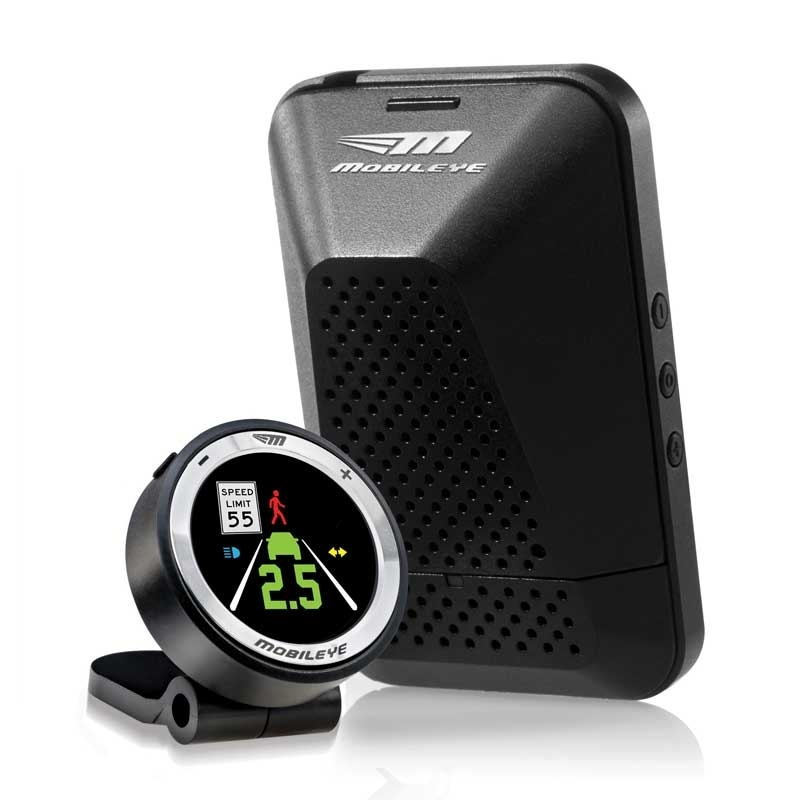
\includegraphics[width=4cm]{figures/4.1.jpg}
    \caption{Mobileye. Fuente: gofleet.com}
    \label{fig:4.1}
\end{minipage}
\begin{minipage}{.5\textwidth} 
\setlength{\parskip}{0.2cm}
\textbf{CARACTERÍSTICAS MOBILEYE}
\begin{itemize}
    \item Frecuencia de detección: 10 Hz
    \item Distancia de alcance: 150 metros
    \item Ángulo de visión horizontal: 74º
    \item Reconocimiento de señales
    \item Reconocimiento del tipo de vehículo
    \item Reconocimiento del estatus del vehículo
\end{itemize}
\end{minipage}
\end{figure}

Por otro lado, la tecnología \gls{lidar} se basa en un láser rotativo para detección de objetos y posterior transformación en una nube de puntos. Los haces de luz proyectan sobre los elementos del entorno, devolviendo a su regreso las variables de posición en el espacio y de intensidad, la cual es dependiente de la reflectividad de cada cuerpo y muy útil para la identificación de diferentes materiales.

El \gls{lidar} utilizado consta de 64 haces o capas, del fabricante Ouster versión OS1 (Figura \ref{fig:4.2}), y se ubica en el techo del vehículo mediante una fijación mecánica. A continuación, se detallan las características del Ouster OS-1.

\newpage
\begin{figure}[htb]
\centering
\begin{minipage}{.4\textwidth}
    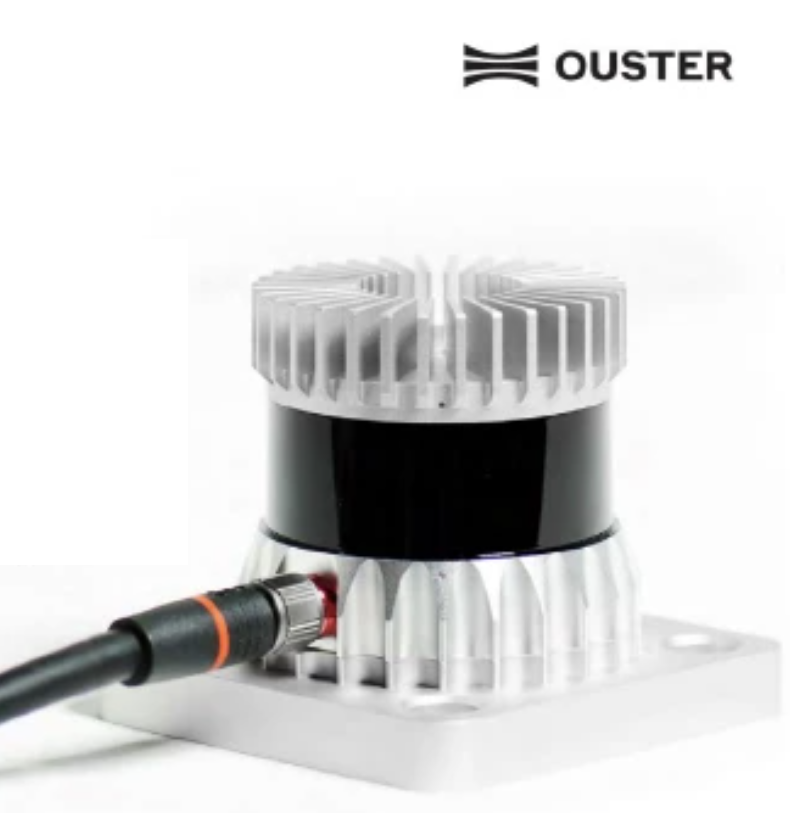
\includegraphics[width=4cm]{figures/4.2.png}
    \caption{Ouster OS1. Fuerte: Ouster/General Laser}
    \label{fig:4.2}
\end{minipage}
\begin{minipage}{.5\textwidth} 
\setlength{\parskip}{0.2cm}
\textbf{CARACTERÍSTICAS OUSTER OS-1}
\begin{itemize}
    \item Frecuencia de rotación: 10 Hz o 20 Hz
    \item Distancia de alcance: 120 metros
    \item Resolución horizontal: 512, 1024 o 2048
    \item Ángulo de visión: 45º (±22.5º)
    \item Resolución angular vertical: 0.35º - 2.8º
    \item Precisión: ±0.7 – 5 centímetros
    \item Puntos por segundo: 1310720
\end{itemize}
\end{minipage}
\end{figure}

Los datos obtenidos del \gls{lidar} se expresan en forma de nube de puntos que se registran por cada frame que captura. Para el correcto análisis de los puntos, es preciso utilizar un algoritmo de clusterización o agrupamiento que nos permita conocer el centro geométrico de cada obstáculo en el espacio. Los algoritmos de clusterización tienen como objetivo formar subgrupos o clusters sobre un conjunto de datos según criterio. Para ello se ha hecho uso del algoritmo planteado en \textcite{clavijo} basado en el método DBSCAN (\gls{dbscan}) adaptado a láseres rotativos, en el que se propone implementar una densidad de puntos variable en función de la distancia al origen. Esta modificación permite aumentar la identificación de clusters de 10 a 40 metros (Figura \ref{fig:4.3}), lo cual favorece directamente a la detección de obstáculos en los ensayos de conducción en vías de alta capacidad propuestos en esta Tesis.

\begin{figure}[h]
    \centering
    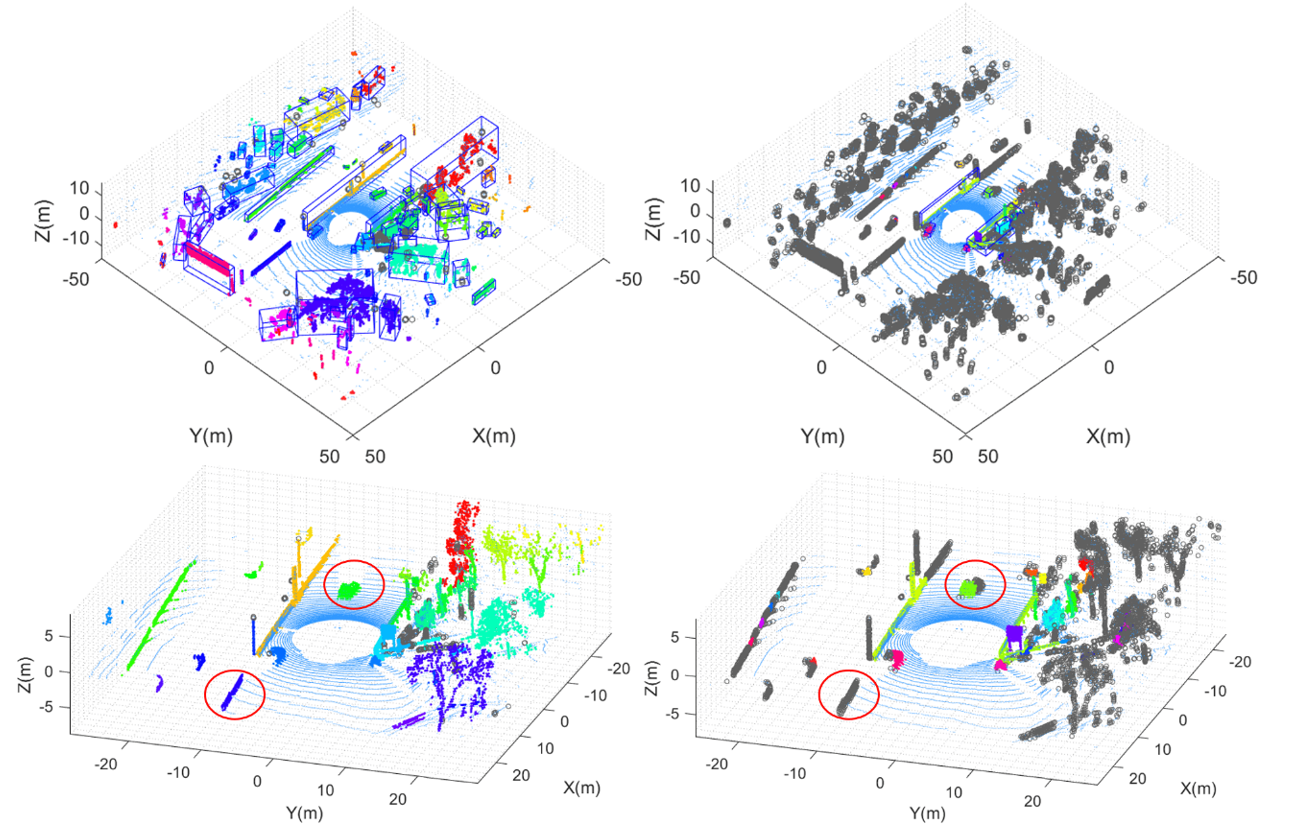
\includegraphics[width=12.5cm]
    {figures/4.3.png}
    \caption{ \label{fig:4.3} Mejora en el funcionamiento del algoritmo de detección en láseres rotativos (\cite{clavijo})}
\end{figure}

El análisis de la mirada se realizó utilizando el sistema de seguimiento visual Tobii Pro Glasses 2 descrito en el subapartado \hyperref[3121]{3.1.2.1.}

Por último, para conocer el movimiento de la cabeza, se elaboró un sistema basado en infrarrojos. El emisor se compuso de tres indicadores lumínicos (Figura \ref{fig:4.4}) montados sobre una gorra junto al circuito integrado y la batería, la cual llevaría el conductor durante los ensayos (Figura \ref{fig:4.6}) basándonos en el sistema de TrackHat. Para el receptor se utilizó una pequeña cámara HD tipo webcam (Figura \ref{fig:4.5}) fácilmente instalable en cualquier parte del vehículo, a la cual se le incorporó un filtro infrarrojo proveniente del Wiimote (Figura \ref{fig:4.7}) que opera en longitudes de onda superiores a 850nm. Las especificaciones de los componentes se adjuntan a continuación.

\begin{figure}[htb]
\centering
\begin{minipage}{.4\textwidth}
    \centering
    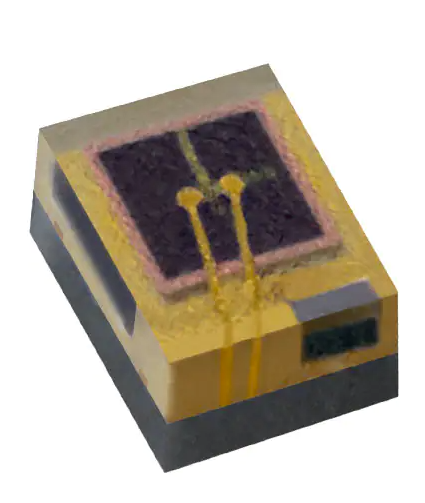
\includegraphics[width=3cm]{figures/4.4.png}
    \caption{LED IR de montaje superficial}
    \label{fig:4.4}
\end{minipage}
\begin{minipage}{.5\textwidth} 
\setlength{\parskip}{0.2cm}
\textbf{CARACTERÍSTICAS LED IR}
\begin{itemize}
    \item Longitud de Onda de Pico: 940 nm
    \item Flujo Radiante: 1.150mW
    \item Intensidad Radiante: 300mW/sr
    \item Tipo de Montaje: Superficial
    \item Ángulo de Intensidad Media: 150º
    \item Tensión de Alimentación Máxima: 3.4V
\end{itemize}
\end{minipage}
\end{figure}

\begin{figure}[htb]
\centering
\begin{minipage}{.4\textwidth}
    \centering
    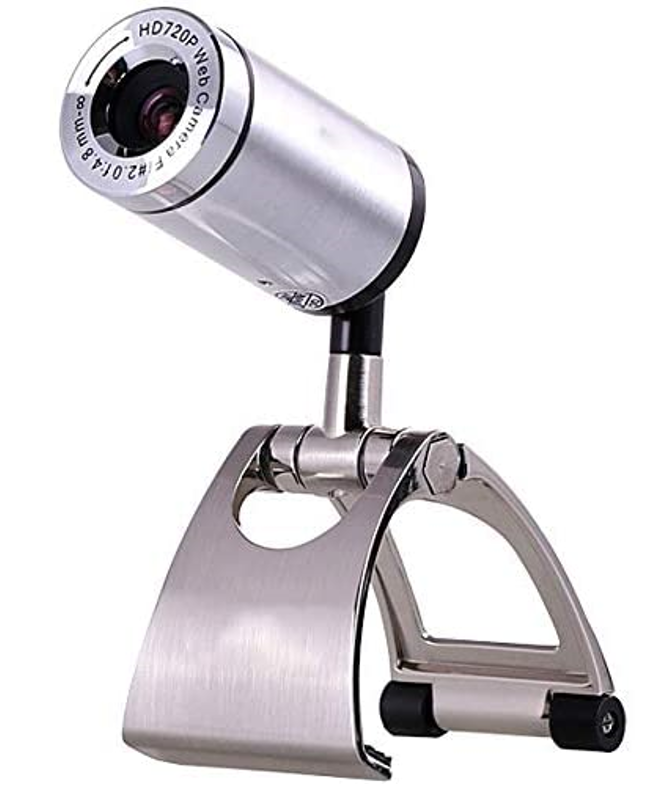
\includegraphics[width=3cm]{figures/4.5.png}
    \caption{WebCam}
    \label{fig:4.5}
\end{minipage}
\begin{minipage}{.5\textwidth} 
\setlength{\parskip}{0.2cm}
\textbf{CARACTERÍSTICAS WEBCAM}
\begin{itemize}
    \item Resolución de Video: 1280 x 720
    \item Modo de Video: YUY2/MJPG
    \item Iluminación Mínima: 10lux
    \item Frames por Segundo: 30fps
    \item Conexión: USB2.0/USB1.1
    \item Alimentación: 5V
\end{itemize}
\end{minipage}
\end{figure}

\begin{figure}[h]
  \centering
  \begin{subfigure}[b]{0.40\textwidth}
    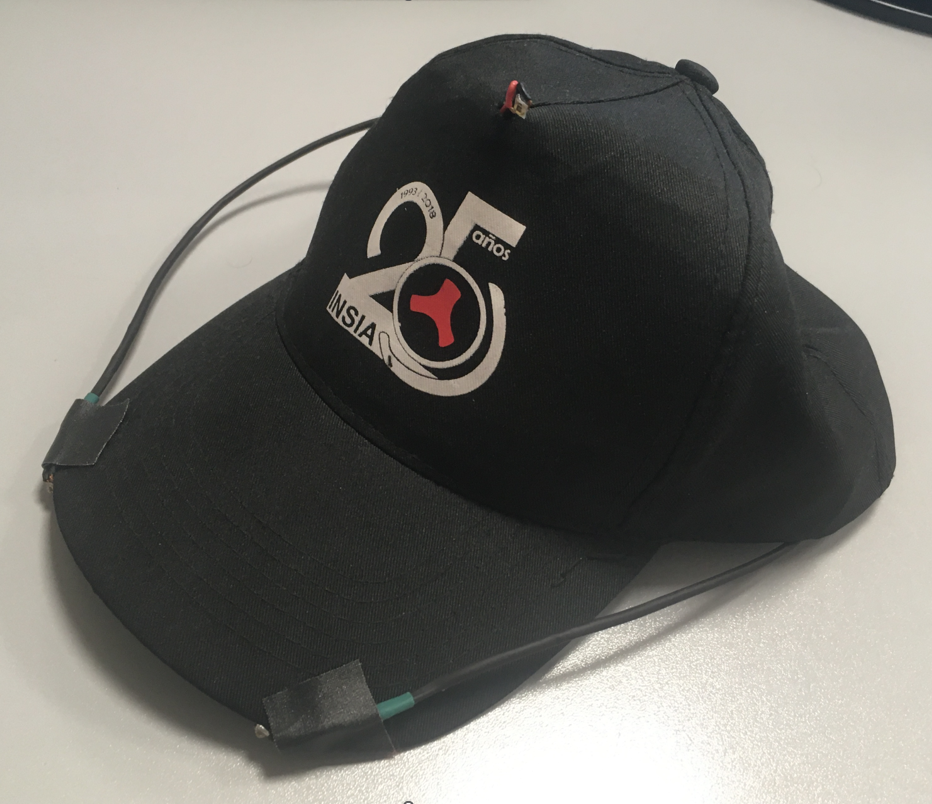
\includegraphics[width=5.5cm]{figures/4.6a.png}
    \caption{}
    \label{fig:4.6a}
  \end{subfigure}
  \hfill
  \begin{subfigure}[b]{0.4\textwidth}
    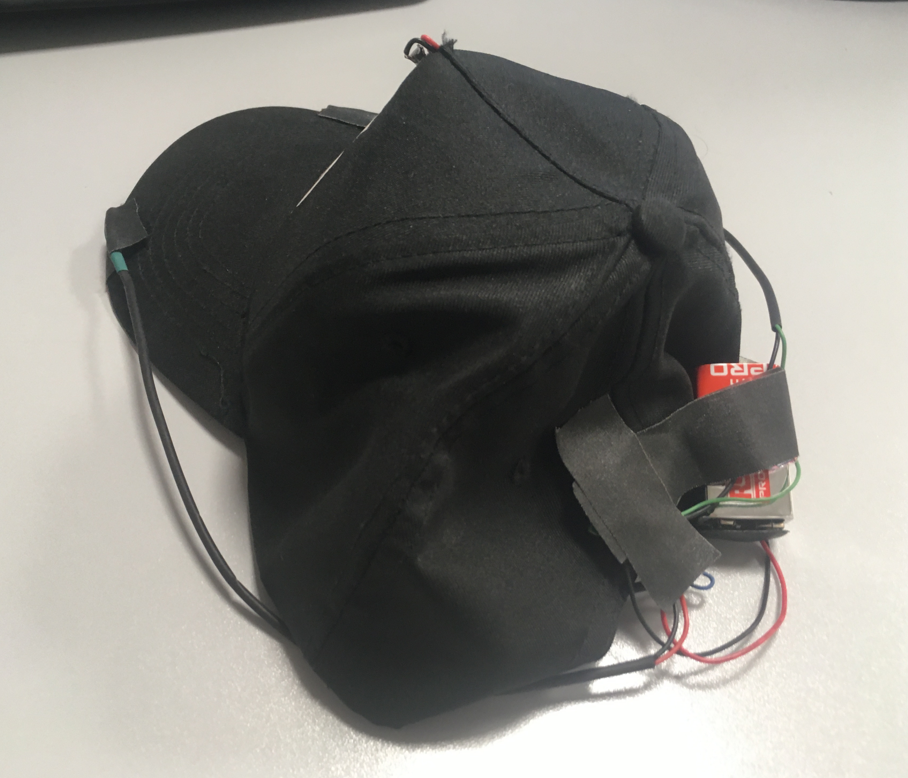
\includegraphics[width=5.5cm]{figures/4.6b.png}
    \caption{}
    \label{fig:4.6b}
  \end{subfigure}
  \caption{Montaje de los infrarrojos sobre gorra. (a) Vista frontal. (b) Vista trasera}
  \label{fig:4.6}
\end{figure}

\begin{figure}[h]
    \centering
    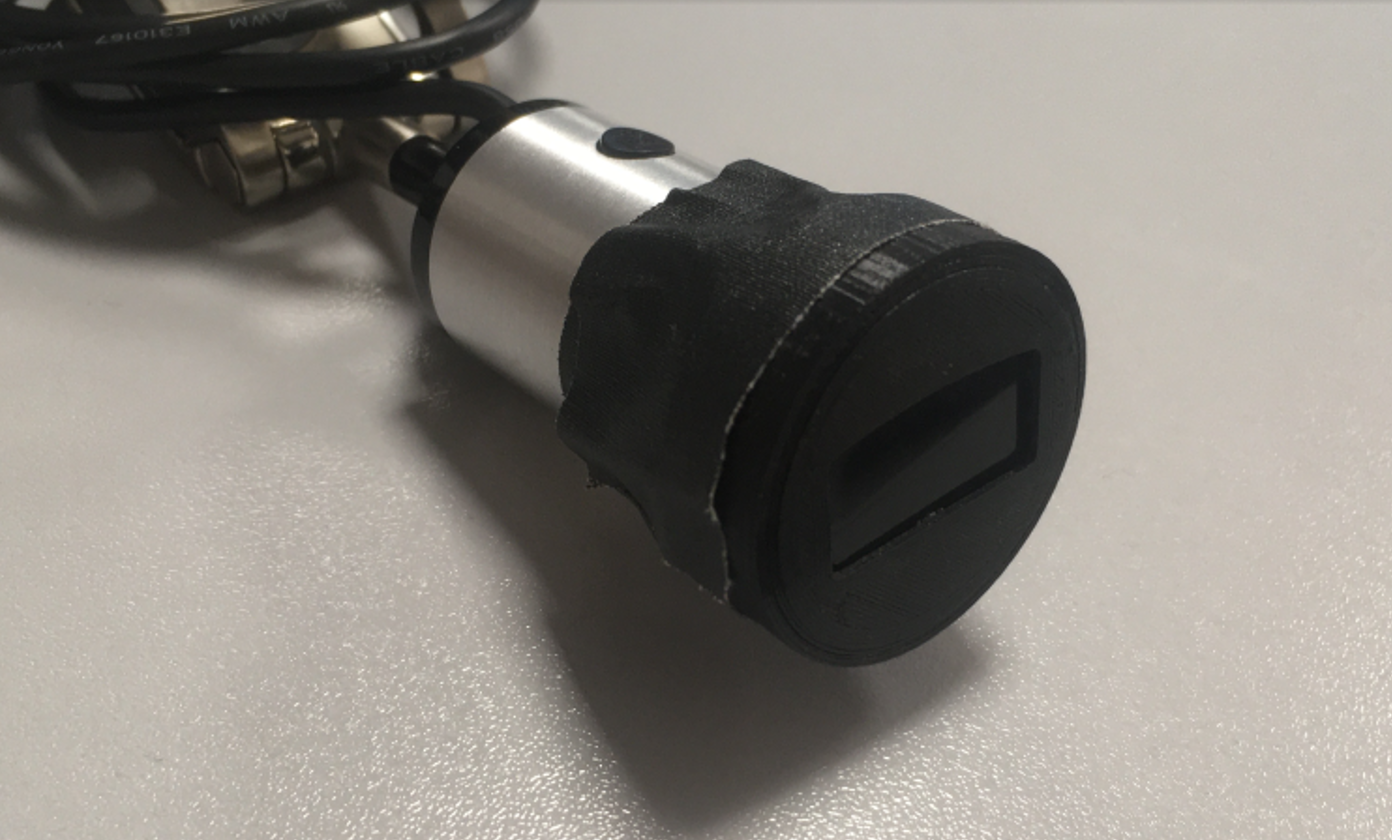
\includegraphics[width=10cm]
    {figures/4.7.png}
    \caption{ \label{fig:4.7} Cámara Webcam}
\end{figure}

La instalación de la cámara se realiza en el salpicadero del vehículo (Figura \ref{fig:4.8}), pudiendo detectar la cabeza del conductor en un amplio rango de movimientos al igual que los sistemas basados en reconocimiento facial, con la ventaja de solo disponer de una única cámara debido al sistema de infrarrojos. 

\begin{figure}[hb]
    \centering
    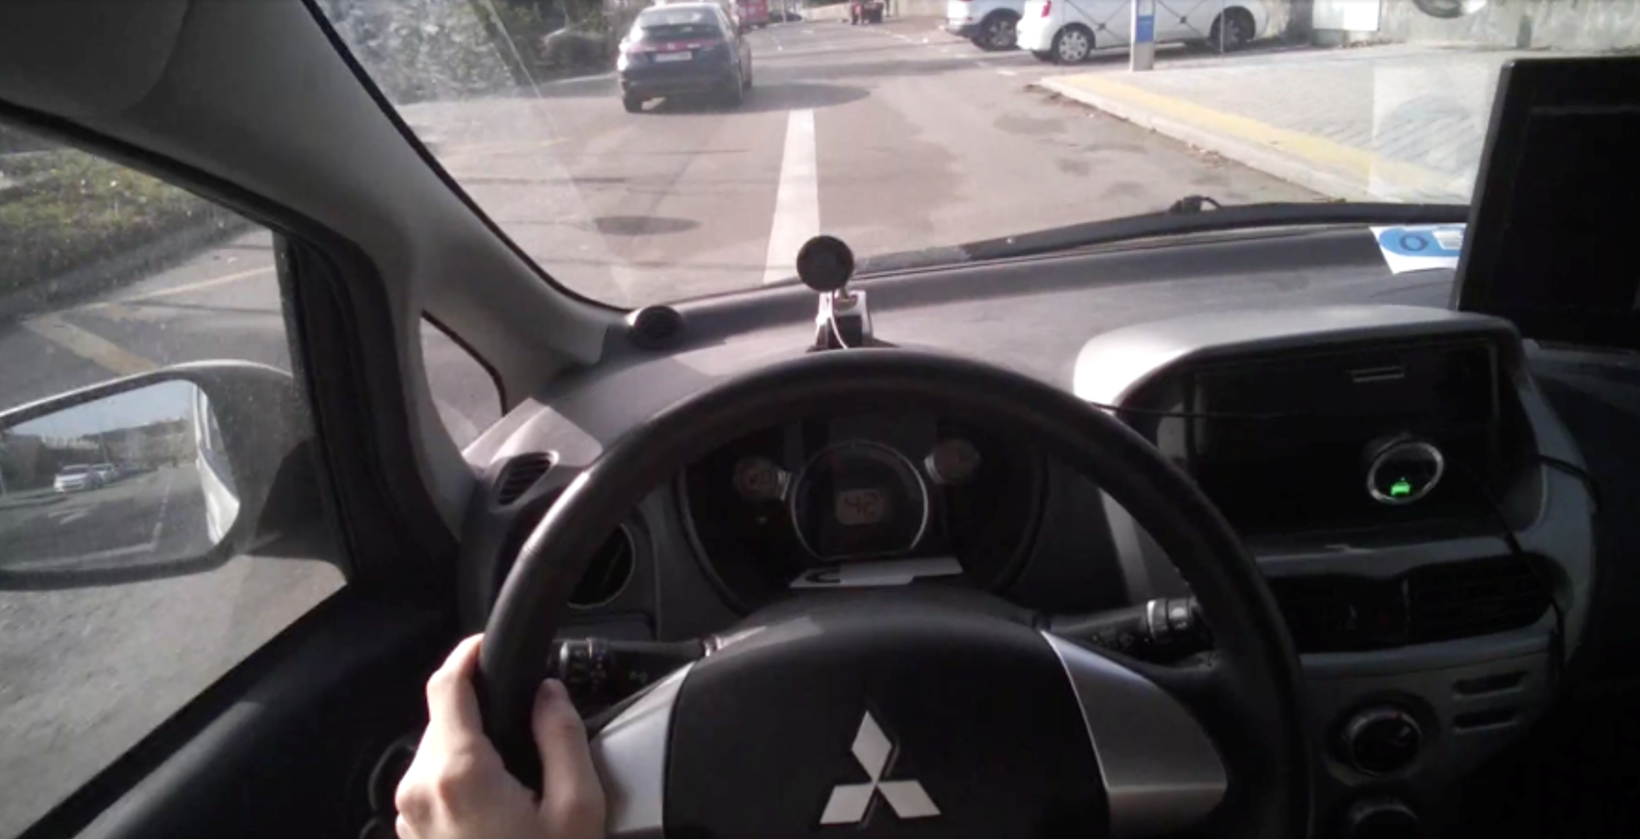
\includegraphics[width=11cm]
    {figures/4.8.png}
    \caption{ \label{fig:4.8} Montaje de la cámara en el interior del vehículo}
\end{figure}

Para la detección de los tres indicadores infrarrojos se optó por el software de código libre y gratuito Opentrack (\cite{opentrack}), comúnmente utilizado en el sector de los videojuegos destacando por su estabilidad y su interfaz configurable frente a otros softwares de pago. El programa realiza una triangulación de dimensiones fijas de los tres indicadores lumínicos detectados y calcula los ángulos de guiñada, alabeo y cabeceo, además de la traslación en los ejes XYZ. Previamente, se realiza una breve configuración donde se especifica que la distribución de los infrarrojos será encima de una gorra y las distancias entre los mismos. Además de trabajar en tiempo real, Opentrack es capaz de exportar los datos de la grabación para poder trabajar con ellos a posteriori. Los datos se muestran tanto en bruto como tras un filtro y un suavizado personalizables, que favorecen la linealidad de los resultados y eliminan ruido y valores pico de la adquisición. Para los ensayos se ha utilizado el Filtro \emph{“Accela”}, con valores de 0.03º para zona muerta y de 1.5º de suavizado para rotación, y de 0.1 milímetros de zona muerta y 1 milímetro de suavizado para traslación. A su vez, se realizan ajustes en los ejes de coordenadas para una buena compenetración con los datos obtenidos del sistema de seguimiento visual. 

Todos los sensores son referenciados y ubicados en un vehículo instrumentado, concretamente el Mitsubishi iMiEV que se puede observar en la figura \ref{fig:4.9}.

\begin{figure}[h]
    \centering
    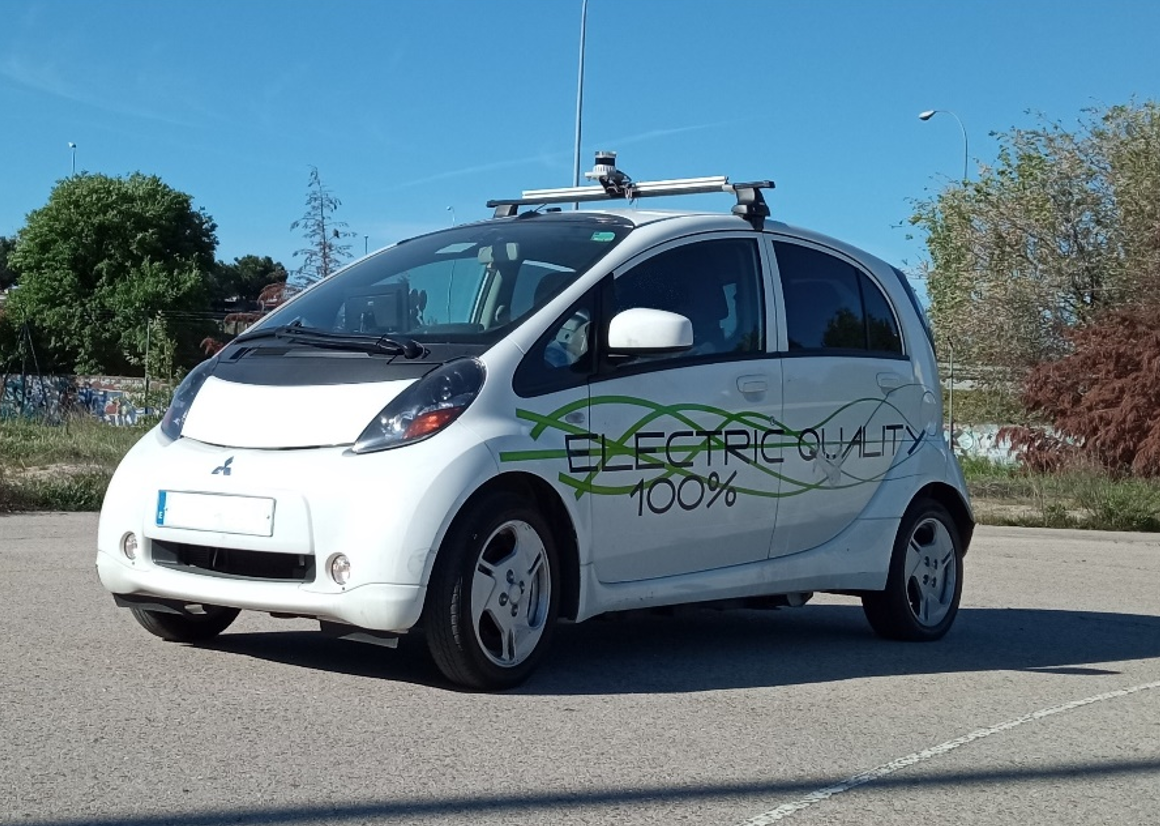
\includegraphics[width=9cm]
    {figures/4.9.png}
    \caption{ \label{fig:4.9} Vehículo Mitsubishi iMiEV instrumentado}
\end{figure}

Los sistemas se conectan a un ordenador encargado del bajo nivel, basado en el sistema operativo GNU/Linux con el entorno de trabajo ROS (Robotic Operating System). La creación de un reloj temporal común a todos los sistemas y la adquisición a la misma frecuencia han sido las principales razones para la elección de este entorno de desarrollo.
Además de los sistemas mencionados anteriormente, se recogerán datos del BUSCAN, para conocer las variables del vehículo, y de un receptor \gls{gps} Trimble R4, instalado en el vehículo para mejorar conocer el posicionamiento del vehículo en los ensayos.

\section{Ajuste y comprobación del sistema de percepción del conductor }\label{43}

Previo al análisis de correlación de la mirada del conductor en el espacio, se realizaron una serie comprobaciones y ajustes de los sistemas de percepción del conductor expuestos en este capítulo, donde se evalúa la integración del sistema de seguimiento de la cabeza junto a los datos de seguimiento visual, calculando la precisión o repetibilidad, y la exactitud resultante en el sistema de coordenadas global.

\subsection{Proyección de la mirada en el sistema de coordenadas global}\label{431}

El sistema de seguimiento visual empleado proporciona la capacidad de exportar numerosas variables en diversos formatos, en concreto la dirección de la dirección de la mirada en el sistema de coordenadas global en 2D, en los ejes XY, y en 3D, en los ejes XYZ. A pesar de que la mirada en 2D está en formato pixeles y la mirada en 3D en metros, una superposición de los datos en el plano XY debería proporcionar una imagen similar en ambos formatos. Sin embargo, al observar diferencias entre ambos formatos, se procedió a analizar la adquisición del sistema con el fin de asegurar una fuente de datos óptima.

Para evaluar la correlación entre las variables de la mirada en 2D y 3D se propone el siguiente ensayo, replicando el procedimiento que el fabricante realizó para la determinación de la exactitud y precisión, o repetibilidad (\cite{tobii}). Los participantes deben de mirar a 4 dianas en forma de cruz ubicadas en una pared estática con una quinta diana de referencia en el centro. Dado que las gafas disponen de una resolución de 1920 x 1080 píxeles, se procede a calcular la distancia necesaria para la realización del ensayo, asegurando que la imagen capturada por la cámara tenga las mismas medidas en milímetros que en píxeles. Esta distancia es de 1.1 metros, encontrándose además dentro del rango óptimo de valores que defiende el fabricante para la obtención de buenos resultados (máximo 3 metros de distancia al objetivo observado (\cite{tobii}). Los ángulos que forman las dianas con la horizontal son 5º, 10º, 15º y 20º, tal y como se muestra en la figura \ref{fig:4.10}, y se restringe el movimiento de la cabeza para analizar puramente la dirección de la mirada.

\begin{figure}[h]
    \centering
    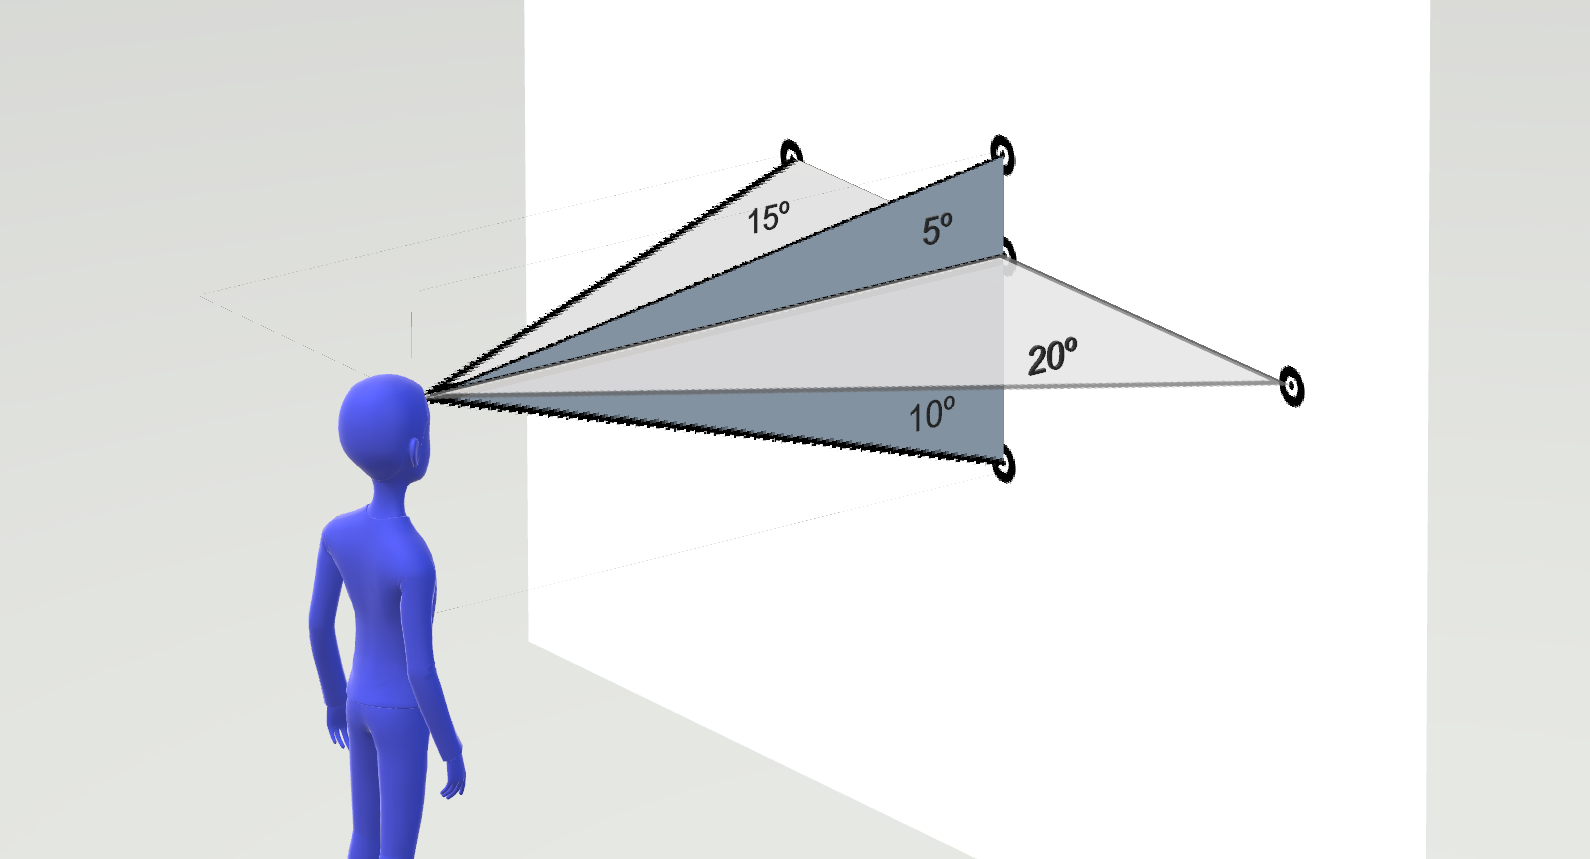
\includegraphics[width=9cm]
    {figures/4.10.png}
    \caption{ \label{fig:4.10} Posicionamiento de las dianas para integración del sistema de percepción del conductor}
\end{figure}

En la siguiente imagen (Figura \ref{fig:4.11}) se observa que existen diferencias notables entre las dos variables, aun perteneciendo ambas al mismo ensayo, correspondiente al sujeto piloto.

\vspace{-10pt}
\begin{figure}[h]
    \centering
    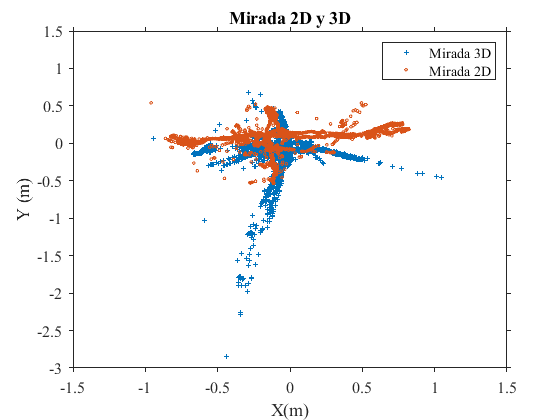
\includegraphics[width=10cm]
    {figures/4.11.png}
    \caption{ \label{fig:4.11} Posición de la mirada en 2D y 3D en ensayo piloto}
\end{figure}

La razón por la que se produce este fenómeno fue revelada analizando la posición de la variable en el eje Z (profundidad en este caso). Se observa que el haz que proyecta la mirada del conductor hacia un objeto detectaba dicho punto mucho más lejos de lo que realmente esta, viéndose también distorsionadas por trigonometría las distancias en los ejes X e Y.
En la figura \ref{fig:4.12} se puede observar el valor de la distancia en el eje Z para el ensayo anterior, donde se muestra que los datos son erráticos e inestables en ciertos puntos, estando la línea de tendencia de la gráfica a 0.841 metros, valor próximo a los 1.1 metros a los que se realiza el ensayo.

\vspace{-15pt}
\begin{figure}[h]
    \centering
    \includegraphics[width=9cm]
    {figures/4.12.png}
    \caption{ \label{fig:4.12} Distancia en profundidad eje Z en ensayo piloto}
\end{figure}

Para solventar este problema, se propone forzar la variable de profundidad en el eje Z a la distancia fija de 1.1 metros a la que se realizó el ensayo anterior, dado que los puntos en este eje no pueden ser superiores a este valor, y se calcula por trigonometría los valores del haz en los ejes X e Y. Los resultados se ven reflejados en la figura \ref{fig:4.13}, donde la posición de la mirada en 3D ha sido corregida, observándose un patrón similar al registrado por las variables en 2D.

\vspace{-15pt}
\begin{figure}[h]
    \centering
    \includegraphics[width=10cm]
    {figures/4.13.png}
    \caption{ \label{fig:4.13} Posición de la mirada en 2D y 3D corregida}
\end{figure}

\newpage
\subsection{Integración del sistema de movimiento de la cabeza }\label{432}

El sistema de coordenadas global de los ensayos propuestos en la presente Tesis tiene su cero en la base de la cabeza del conductor, donde se producen los giros en los tres ejes. El sistema de seguimiento de la cabeza genera variables de los ángulos de rotación y de la translación en XYZ. Estas variables realizan la corrección de los datos de la mirada que se resuelve mediante un sistema matricial, donde, por una parte, se transforman los ángulos con la matriz de rotación de Euler (Eq. \ref{eq:4}), y posteriormente se aplica una matriz de traslación (Eq. \ref{eq:5}). Los datos del sistema de seguimiento visual (Eq. \ref{eq:6}) son multiplicados matricialmente por la matriz de transformación compuesta por la rotación y la translación como se observa en la ecuación \ref{eq:7}.


\begin{equation}\label{eq:4}
\text{Euler} = \begin{bmatrix}
\alpha_x & \beta_x & \gamma_x \\
\alpha_y & \beta_y & \gamma_y \\
\alpha_z & \beta_z & \gamma_z
\end{bmatrix}
\end{equation}

\begin{equation}\label{eq:5}
\text{Posición} = \begin{bmatrix}
X_n \\
Y_n \\
Z_n
\end{bmatrix}
\end{equation}

\begin{equation}
\text{Visual} = \begin{bmatrix} \label{eq:6}
x_n \\
y_n \\
z_n \\
1
\end{bmatrix}
\end{equation}

\begin{equation}\label{eq:7}
\text{Correc}_1 = \left[ \text{Euler} | \text{Posición} \right] \cdot \left[ \text{Visual} \right] = \left[ \left[ \begin{array}{@{}c@{}}
\text{Matriz} \\
\text{Rotación} \\ 
\text{Euler} \\
\end{array} \right] \left( \begin{array}{@{}c@{}}
X_n \\
Y_n \\
Z_n \\
\end{array} \right) \right] \cdot \left[ \left( \begin{array}{@{}ccc@{}}
x_n \\
y_n \\
z_n \\
1  \\
\end{array} \right) \right]
\end{equation}

Sabiendo que la incertidumbre de ambos sistemas es alta, pero está dentro de los limites admisibles, se realiza una evaluación meramente cualitativa de la fusión con objeto de comprobar la bondad del sistema desarrollado. Para ello se propone calcular la repetibilidad y la exactitud del ensayo de 4 dianas mencionado anteriormente, para una muestra reducida de 3 sujetos (\emph{N}). La repetibilidad y la exactitud son recursos comúnmente utilizados para la evaluación del error obtenido en sistemas de medición, como se puede apreciar en \textcite{holmqvist}, con la validación de la calidad de los sistemas de seguimiento visual. La exactitud se define como la cercanía de las medidas obtenidas al valor real, mientras que la repetibilidad es el grado de proximidad entre las mediciones. Para la exactitud se toma como referencia la medida real y para la repetibilidad, el centroide de la nube de puntos. Ambas variables indican diferentes aspectos y, por tanto, son independientes, pudiéndose obtener una muestra muy precisa, donde todas las medidas difieren poco entre sí, pero poco exacta si está lejos del valor real.

En la tabla \ref{tab:4.1}, se muestran los resultados obtenidos de la fusión sensorial para el ensayo de las cuatro dianas mencionado anteriormente.

\newpage
\begin{table}[h]
\centering
\begin{tabular}{cccccc}
\multirow{2}{*}{\textbf{Grados (°)}} & \multirow{2}{*}{\textbf{N}} & \multicolumn{2}{c}{\textbf{Exactitud (°)}} & \multicolumn{2}{c}{\textbf{Repetibilidad (°)}} \\ \cline{3-6} 
                                     &                             & \textit{Media}        & \textit{SD}        & \textit{Media}          & \textit{SD}          \\ \hline
5                                    & 3                           & 3.86                  & 3.15               & 3.70                    & 2.44                 \\ \hline
10                                   & 3                           & 2.85                  & 1.33               & 1.06                    & 0.80                 \\ \hline
15                                   & 3                           & 1.51                  & 0.65               & 1.60                    & 0.84                 \\ \hline
20                                   & 3                           & 2.14                  & 0.79               & 0.74                    & 0.52                 \\ \hline
\end{tabular}
\caption{Exactitud y repetibilidad del sistema de percepción del conductor}
\label{tab:4.1}
\end{table}

\vspace{-15pt}
Como era de esperar, la exactitud y la repetibilidad del sistema de seguimiento visual se ven afectadas por la inclusión del sistema de seguimiento de la cabeza. Se observa que los peores resultados se obtienen para el valor de 5°, lo cual puede ser explicado por la proximidad a la diana central y la atracción de la mirada hacia un elemento próximo y similar al objetivo visual. Esta afirmación se refuerza con el valor de dispersión obtenida para esa medida. Otro aspecto a considerar es el número de sujetos, ya que se considera que una mayor población en las muestras adquiridas enriquecería de manera notable los resultados. 

A pesar de las desviaciones detectadas, se puede concluir que la fusión sensorial es más precisa que exacta, donde los datos se agrupan correctamente, pero difieren de la medida real. No obstante, los valores se consideran válidos para la aplicación propuesta, dado que a la distancia máxima operable (50 metros) la desviación supondría 3.3 metros en el peor de los casos, siendo inferior al ancho de un carril de 3.5 metros. 

\section{Análisis de correlación con percepción del entorno}\label{44}
La integración de los sistemas de detección del entorno, la cámara Mobileye y el láser Ouster, ya ha sido estudiada con anterioridad en \textcite{villacieros}, observado ciertas carencias en la redundancia conjunta debido a la naturaleza de los mismos. Por un lado, la versión utilizada para la cámara Mobileye tiene un ángulo de visión horizontal de 74°, por lo que la máxima amplitud de detección para objetos que se sitúan en el lateral del vehículo es de 36°. Además, la localización de obstáculos es menos flexible respecto a la del Ouster, por lo que no permite una buena adaptabilidad a los cambios. Respecto al sensor láser, a pesar de la mejora del algoritmo de clusterización (\cite{clavijo}), es un hecho que, a mayor distancia de detección, mayor distancia entre haces consecutivos, siendo esta una de las principales razones de la pérdida de objetos en el campo visual. 

Debido a las limitaciones presentadas, se propuso en primer lugar, un análisis en la correlación en la detección de obstáculos de la cámara Mobileye y el láser Ouster, y posteriormente, la integración total con el sistema de seguimiento visual.

\subsection{Metodología }\label{441}
Dos vehículos instrumentados realizaron una maniobra de seguimiento de vehículo (car-following) en un entorno abierto, correspondiente a una carretera de urbana. Se realizaron 5 repeticiones del mismo recorrido, detectando al vehículo delantero mediante la cámara Mobileye y el láser Ouster durante todo el ensayo. 

Por otro lado, se registraron datos del conductor a través del sistema de seguimiento visual y se estudió el campo visual del conductor. La visión humana se compone de un campo visual central, correspondiente a la zona de máxima agudeza visual, y un campo visual periférico, situado a los laterales de la zona central y que también aporta información visual al cerebro, pero de manera menos precisa. A menudo, en entornos de conducción, el ángulo de visión central se ve afectado por la velocidad del vehículo, viéndose reducido y repercutiendo directamente en la toma de decisiones. Este fenómeno denominado ``efecto túnel'' y ampliamente estudiado (\cite{edwards}) ha sido integrado en el análisis de correlación para el sistema visual, considerando esta variable como un rango de incertidumbre admisible en la detección de la mirada del conductor.

\subsection{Resultados }\label{442}
El análisis de correlación de los sistemas se calculó en porcentaje de frames de detección frente al número total de frames de la grabación. Primero se calculó la coincidencia entre los sistemas de percepción, cámara y \gls{lidar}, y posteriormente se añadió el sistema de seguimiento visual en el sistema de coordenadas global. 

Un ejemplo de ello se observa en el frame mostrado en la figura \ref{fig:4.14}, donde aparecen todos los sistemas desde la perspectiva de planta, ubicándose el vehículo instrumentado en el punto (0, 0). Los obstáculos detectados por la cámara aparecen con un asterisco rojo, en este caso solo existe el vehículo delantero y el vehículo instrumentado en el centro. Los demás objetos son el resultado de la detección con el láser y el algoritmo de clusterización \gls{dbscan}, mencionado en el apartado \ref{42} instrumentación y procesamiento de datos. En este ejemplo se puede observar que la detección con la cámara coincide con uno de los clusters determinados por la detección del láser. Las líneas verticales representan la dirección de la mirada del conductor, partiendo desde el centro hacia delante, siendo el resultado de la integración del sistema de seguimiento visual y el sistema de movimiento de la cabeza. El triángulo azul muestra el ángulo central de visión del conductor, el cual pivota según la dirección de la mirada y cambia su apertura en función de la velocidad del vehículo, englobando la dispersión de miradas admisibles.

Como se observa en la figura \ref{fig:4.14}, dentro de este ángulo se encuentra la dirección de la mirada y el vehículo delantero.

\vspace{-20pt}
\begin{figure}[h]
    \centering
    \includegraphics[width=9.5cm]
    {figures/4.14.png}
    \caption{ \label{fig:4.14} Mirada del conductor a un obstáculo mediante la fusión de todos los sistemas}
\end{figure}

\newpage
Los porcentajes de detección de frames para la cámara Mobileye, el láser Ouster y la detección conjunta, se muestran en la siguiente tabla \ref{tab:4.2}, donde los resultados de la detección conjunta son relativamente bajos y destaca positivamente la detección realizada por la cámara Mobileye.

\begin{table}[h]
\centering
\begin{tabular}{cccccc}
\textbf{Ensayo}       & \textbf{1}   & \textbf{2}     & \textbf{3}     & \textbf{4}     & \textbf{5}     \\ \hline
\% detección Mobileye & 100 & 87.31 & 73.05 & 92.43 & 95.18 \\ \hline
\% detección Ouster   & 81.36        & 74.02          & 65.25          & 58.37          & 100            \\ \hline
\% detección conjunta & 81.36        & 61.93          & 39.01          & 50.81          & 95.18         
\end{tabular}
\caption{Porcentaje de correlación en frames de Mobileye y Ouster}
\label{tab:4.2}
\end{table}

De igual manera, los resultados se muestran en porcentajes de frames detectados respecto al total de frames, mostrando por un lado la coincidencia de miradas al obstáculo detectado, y por otro, la coincidencia de miradas dentro del ángulo de visión central en función de la velocidad y el giro de la cabeza (Tabla \ref{tab:4.3}). Los haces de la mirada se han distribuido en grupos de cinco, debido a que el registro de la actividad ocular funciona a 50 Hz, cinco veces superior al resto de los sistemas, considerándose suficiente muestreo para este análisis. 

\begin{table}[h]
\centering
\begin{tabular}{cccccc}
\textbf{Ensayo}                                          & \textbf{1} & \textbf{2} & \textbf{3} & \textbf{4} & \textbf{5} \\ \hline
\% coincidencia de miradas al   obstáculo                & 13.66      & 38.67      & 58.86      & 32.97      & 39.01      \\ \hline
\% coincidencia de miradas en   ángulo de visión central & 59.62      & 93.95      & 99.29      & 96.21      & 88.83      \\ \hline
\end{tabular}
\caption{Porcentaje de correlación en \\ frames del sistema de seguimiento visual}
\label{tab:4.3}
\end{table}

Los valores obtenidos indican que el conductor realiza la mayor parte de las miradas dentro del ángulo de visión central y, como mínimo un 30\% de las miradas al obstáculo en concreto, exceptuando el ensayo 1 en ambos casos. Los valores más bajos se debieron a diversos problemas en la adquisición de la mirada, como es el caso del ensayo 1, donde se dieron situaciones en las que el conductor giraba en exceso la cabeza, perdiendo una de las señales de triangulación del sistema de seguimiento y proyectando los haces de la mirada de manera incorrecta. A pesar de que se eligieron sensores infrarrojos por su buena adaptabilidad a las diferencias lumínicas, el exceso de luz en ciertas zonas junto a destellos puntuales también afectó a la descalibración del sistema, traduciéndose en una pérdida parcial de los datos.

\subsection{Discusión}\label{443}
La detección de obstáculos es una función crítica para la seguridad en el manejo de vehículos. En este estudio se realizaron ensayos de detección en conducción real fusionando dos sistemas de percepción del entorno y un sistema de seguimiento visual, referenciado al sistema de coordenadas global a través de un sistema de seguimiento de la cabeza.

En los resultados obtenidos sobre el análisis de correlación se encontró que la detección para la cámara Mobileye fue alta, pero que debido a la baja detección del \gls{lidar} Ouster relacionada con la clusterización de obstáculos a largas distancias, la efectividad conjunta se vio mermada de manera general. Con respecto al análisis de la fusión junto al sistema de seguimiento visual, se presupone que el conductor dedicará gran parte de su atención al vehículo que circula delante de él. Sin embargo, esta hipótesis no es del todo cierta ya es posible adquirir información de la escena sin necesidad de mirar directamente al obstáculo que se encuentra en frente, como se puede ver en los resultados obtenidos de miradas en el ángulo de visión central calculado a través del “efecto túnel”. Los resultados obtenidos mostraron que un gran porcentaje de las miradas coincidieron con el ángulo de visión central pero solo un tercio de las mismas alcanzaron al vehículo delantero. 

\section{Conclusiones}\label{45}
La conducción autónoma se basa principalmente en la adquisición de información del entorno a través de diferentes sensores, la cual se procesa como lo haría un conductor humano. La redundancia entre sensores ofrece una mejora en los algoritmos de control, haciendo que la integración de los vehículos en el tráfico mixto sea lo más eficaz posible. Dado que todavía queda mucho conocimiento sobre la conducción humana que implementar, se considera que la proyección de la mirada del conductor hacia el entorno exterior puede aportar una valiosa información en la determinación de reglas del sistema de decisiones.

En este capítulo se ha realizado una fusión sensorial entre dos sistemas de detección de obstáculos y un sistema de seguimiento visual referenciado al sistema de coordenadas global gracias a un sistema para el seguimiento de la cabeza. Este desarrollo ha permitido obtener un conocimiento global de la mirada del conductor hacia el entorno exterior, facilitando su integración con otros sistemas de percepción del entorno. No obstante, el sistema de seguimiento de la cabeza no se considera robusto dado que los resultados muestran problemas en la adquisición de datos debido a sus carencias frente a las variaciones lumínicas y la movilidad del conductor. En futuros estudios se considera interesante la implementación de dos cámaras que capturen dicho movimiento y aporten redundancia a la adquisición.

En los ensayos realizados en conducción real, los sensores de percepción del entorno han tenido buenos resultados en la detección individual, pero mejorables en la detección conjunta, debido a las limitaciones del método de clusterización para el entorno ensayado. Tras la adición del sistema de seguimiento visual referenciado al sistema global se observó que, en la mayoría de los ensayos, la mirada del conductor se encontraba dentro del ángulo central de visión, pero que solo una tercera parte de las mismas se realizaban al obstáculo en concreto. Este hecho refuerza la hipótesis de que el conductor puede recopilar información de la escena sin requerir una visión precisa, recalcando la importancia de la visión periférica.

En el siguiente capítulo se recogerán datos de conducción real, haciendo uso de los desarrollos de fusión obtenidos, para el desarrollo de un modelo de conducción enfocado a la conducción autónoma. 


\makechapter{Modelo de toma de decisiones en conducción autónoma}{Modelo de toma de decisiones en conducción autónoma}{Modelo de toma de decisiones en conducción autónoma\label{ch5}}
Las acciones que realiza un vehículo autónomo tienen dos etapas previas bien definidas, la percepción del entorno y el procesamiento de la información adquirida. En este punto se realiza la toma de decisiones, la cual consiste en un conjunto de reglas que imitan el comportamiento del conductor. Su caracterización mediante modelos de toma de decisiones ayuda al desarrollo de algoritmos más naturalistas que impulsen la integración de los vehículos autónomos en el tráfico mixto. 

Los conductores tienen la capacidad de adaptarse a cualquier entorno por muy cambiante que sea, e incluso anticipar ciertas conductas de los vehículos colindantes de manera intuitiva. Por ello, la observación de la estrategia atencional a través del comportamiento de la mirada es capaz de aportar información tanto sobre el estado como de las intenciones del conductor y sus prioridades en la realización de maniobras.

Con objeto de aportar conocimiento sobre esta cuestión, en este capítulo se ha realiza un modelo de conducción determinista focalizado en situaciones potencialmente conflictivas como adelantamientos en vías de alta capacidad. Para ello, se realizan ensayos experimentales en conducción real, emulando diferentes maniobras en función del número de vehículos en el carril izquierdo. Además, se ha adquirido el comportamiento visual a lo largo de los ensayos propuestos, ya que en el \hyperref[ch3]{Capítulo 3} se concluyó que a través de las variables atencionales se pueden determinar patrones o intenciones del conductor en la gestión de la información del entorno.

A continuación, se presenta la estructura del capítulo. En primer lugar, se realiza una encuesta a nivel exploratorio para conocer los aspectos que son considerados más importantes en la toma de decisiones por los conductores. Posteriormente se desarrolla un modelo de conducción clásico de tipo determinista el cual es ajustado y validado con datos de conducción real en una autovía. La obtención de datos del entorno y del conductor ha sido posible gracias a la fusión sensorial presentada en el \hyperref[ch4]{Capítulo 4}.

\section{Encuesta sobre variables en la toma de decisiones}\label{51}
El objetivo de la encuesta es valorar a nivel exploratorio, qué variables consideran más importantes los conductores en la toma de decisiones en conducción. Dichas variables fueron seleccionadas por ser las más comunes en los modelos de conducción, como se observó en el estado del arte del \hyperref[ch2]{Capítulo 2}, siendo evaluadas de manera individual y contraponiéndolas entre sí. 

Las variables analizadas se agrupan en aceleraciones, velocidades, tiempos, otras características y variables abstractas. El vehículo propio se indica con el subíndice 1, el vehículo que le precede con el subíndice 2, y los vehículos adyacentes situados en el carril izquierdo, con los subíndices A, B y C, siendo A el que estaría aproximadamente a la misma altura que el 1, y B y C los que seguirían detrás de A. Las agrupaciones y variables propuestas se detallan en la siguiente tabla \ref{tab:5.1}.

\begin{table}[h]
\centering
\begin{tabular}{rcc}
\textbf{Grupos}                        & \multicolumn{2}{c}{\textbf{Variables}}                                \\ \hline
\multirow{3}{*}{Aceleraciones}         & Aceleración   propia mínima                              & a\textsubscript{1min}    \\ \cline{2-3} 
                                       & Aceleración   propia máxima                              & a\textsubscript{1max}   \\ \cline{2-3} 
                                       & Deceleración   propia máxima                             & dec\textsubscript{1max} 
                                       \\ \hline
\multirow{4}{*}{Velocidades}           & Velocidad   propia                                       & v\textsubscript{1}       \\ \cline{2-3} 
                                       & Velocidad   del vehículo adyacente                       & v\textsubscript{A}       \\ \cline{2-3} 
                                       & Velocidad   media carril izquierdo                       & v\textsubscript{m}       \\ \cline{2-3} 
                                       & Velocidad   máxima de la vía                             & v\textsubscript{max}     \\ \hline
\multirow{3}{*}{Tiempos}               & Tiempo de   seguridad                                    & T          \\ \cline{2-3} 
                                       & Tiempo entre   los vehículos A y B                       & t\textsubscript{AB}      \\ \cline{2-3} 
                                       & Tiempo entre   los vehículos B y C                       & t\textsubscript{BC}      \\ \hline
\multirow{2}{*}{Otras características} & Número de   obstáculos/tráfico                           & n          \\ \cline{2-3} 
                                       & Altura   vehículo delantero                              & h\textsubscript{2}       \\ \hline
Variables abstractas                   & \begin{tabular}[c]{@{}c@{}}Previsión/   Predicción/ Juicios/ \\ Picaresca/ Agresividad\end{tabular} &            \\ \hline
\end{tabular}
\caption{Variables analizadas en la encuesta de toma de decisiones }
\label{tab:5.1}
\end{table}

Los escenarios se resumen en maniobras de seguimiento de vehículo y cambio de carril. La ruta se supone en una vía de alta capacidad, generalmente una autovía o autopista, donde la velocidad máxima son 120 km/h y el trayecto no requiere ningún cambio de ruta. 

La encuesta consiste en un total de 29 preguntas según la escala Likert de 5 opciones y una respuesta abierta, lanzada a través de la plataforma Google Forms. Las preguntas propuestas se encuentran en el \hyperref[AB]{Anexo B: Encuesta sobre variables en la toma de decisiones en la conducción}. Cada cuestión expone una situación de tráfico compleja donde se plantean dos soluciones contrapuestas, cada una priorizando una variable diferente, y donde el conductor debe de determinar el grado de acuerdo con la afirmación. Las preguntas también contemplan una valoración individual de cada variable mediante enunciados en un contexto de tráfico. 

\subsection{Metodología }\label{511}
La muestra se constituye de una total de 120 hombres y 70 mujeres, con edades comprendidas entre 20 y 80 años (\emph{M} = 35.31, \emph{SD} = 12.29). Un 84.21\% de la población manifestó conducir un turismo como vehículo habitual, recorriendo distancias anuales entre 5000 y 10000 km (19.2\%), 10000 y 20000 km (17.54\%) y mayores de 20000 km (63.25\%).

Las puntuaciones obtenidas en la encuesta reflejan la preferencia de los participantes sobre las variables propuestas durante la tarea de conducción. Las variables fueron puntuadas de manera individual y contraponiéndolas entre sí, realizando todas las combinaciones posibles. Las medias de las puntuaciones obtenidas se trasladaron a porcentajes, considerando relevantes los resultados cuya puntuación fuera mayor del 70\%. De igual manera, en los ítems comparativos se consideraron significativas aquellas parejas donde un extremo fuese por lo menos dos tercios mejor valorado que el otro. 

Las preguntas fueron analizadas estadísticamente, atendiendo al tamaño de la muestra y distribución. Dado que en algunos ítems las variables eran valoradas individualmente y en otros se contraponían entre sí, se propuso la evaluación porcentual de las puntuaciones obtenidas, profundizando posteriormente en las más altas. Tras ello, se realizó una matriz de correlación de Pearson con objeto de hallar posibles relaciones entre las variables propuestas. La dinámica de esta prueba se encuentra descrita en el subapartado \hyperref[3111]{3.1.1.1}.

\subsection{Resultados }\label{512}
Las variables mejor valoradas individualmente fueron la aceleración propia mínima (73.68\%) y la velocidad propia (72.52\%), junto a las variables abstractas de predicción (72.95\%) y la previsión (82.11\%). A nivel comparativo se observó que las variables puntuadas más altas frente a otras fueron la velocidad del vehículo adyacente (90.6\%), el tiempo de seguridad (76.21\%) y el tiempo entre los vehículos B y C (73.47\%). Por otro lado, las diferencias significativas halladas en la correlación de Pearson se realizaron en función de los datos demográficos (Tabla \ref{tab:5.2}), obteniendo los siguientes resultados significativos.

\begin{table}[h]
\centering
\begin{tabular}{rcc}
\textbf{Variables}                                                                             & \textbf{\begin{tabular}[c]{@{}c@{}}Coeficiente de correlación\\  Pearson\end{tabular}} & \textbf{Valor \emph{p}} \\ \hline
\textit{Variables individuales}                                                                & \textit{Edad}                               &                  \\ \hline
Aceleración mínima                                                                             & -0.146                                      & 0.045            \\
Aceleración máxima                                                                             & -0,25                                       & \textless{}0.001 \\
Velocidad media carril izquierdo                                                               & -0.266                                      & \textless{}0.001 \\ \hline
\textit{Variables comparativas}                                                                & \textit{Distancia recorrida}                &                  \\ \hline
\begin{tabular}[c]{@{}r@{}}Tiempo de seguridad frente \\ a velocidad propia\end{tabular}       & 0.143                                       & 0.05             \\
\begin{tabular}[c]{@{}r@{}}Velocidad máxima frente \\ altura vehículo delantero\end{tabular} & -0.177                                      & 0.015            \\ \hline
\end{tabular}
\caption{Coeficientes de correlación de Pearson entre variables para toma de decisiones (p\textless{}0.05)}
\label{tab:5.2}
\end{table}

Como se observa en la tabla \ref{tab:5.2}, existe una correlación inversamente proporcional entre la edad y la distancia recorrida con las variables individuales. Dichas variables apuntan a un perfil de conducción más dinámico en los conductores más jóvenes y poco experimentados. En las variables comparativas, los resultados apuntan a que son propensos a sobrepasar la velocidad máxima de la vía con tal de evitar un vehículo de gran altura y que prefieren no modificar su propia velocidad pese a sacrificar el tiempo de seguridad. No se obtuvieron diferencias en relación con los años de experiencia en conducción ni en el tipo de vehículo.

\subsection{Discusión}\label{513}
La toma de decisiones en conducción es un proceso complejo donde intervienen diversas variables, las cuales el conductor analiza y evalúa antes de ejecutar una maniobra. En este apartado se ha propuesto una encuesta para analizar cuáles son las mejor valoradas por los conductores, obteniendo resultados representativos e interesantes.

Comparando las variables entre ellas se obtuvo que la puntuación más alta fue la velocidad del vehículo adyacente, indicando que las acciones de los demás vehículos influyen significativamente sobre las decisiones del conductor. Este hecho está relacionado directamente con la seguridad hacia los demás ya que, si el vehículo circulase completamente solo, primarían más las variables de aceleración propia mínima y velocidad propia, las cuales obtuvieron puntuaciones altas en la evaluación de variables de manera individual. Esta idea se ve reforzada por la alta valoración positiva de las variables abstractas predicción y previsión.

Estadísticamente se encontraron correlaciones entre la edad, distancia anual recorrida y las variables estudiadas. Los conductores más jóvenes valoraron positivamente las variables aceleración propia mínima, máxima y la velocidad media del carril izquierdo, indicando un perfil más enérgico e impaciente. Por otro lado, se encontraron relaciones entre los conductores de largas distancias recorridas y las variables relativas a la seguridad.  Esta conclusión define a estos conductores como pacientes y cautelosos, dado que prefieren evitar las maniobras arriesgadas, aun viendo velocidad menguada, y son conscientes de las capacidades y la dinámica de los vehículos de mayor altura, como pueden ser camiones o autobuses. 

Los resultados obtenidos son interesantes en el desarrollo del modelo de toma de decisiones presentado en el siguiente apartado. Las variables tiempo de seguridad, velocidad propia y velocidad media del carril izquierdo tomarán especial importancia en las decisiones del algoritmo, al igual que se analizarán en detalle la velocidad del vehículo adyacente y los tiempos entre vehículos en las maniobras realizadas.

\section{Modelo determinista para conducción autónoma }\label{52}
En este apartado se presenta el desarrollo de un modelo determinista para conducción basado en un árbol de decisión, cuyas principales acciones son seguimiento de vehículo y cambio de carril. Dicho modelo posee la misma estructura que el sistema de ayuda a la incorporación desarrollado en el subapartado \ref{313}, basado en la aceptación de huecos para la realización de maniobras seguras. 

Las decisiones determinadas por el modelo son dependientes de las variables velocidad, distancia y tiempo de cada vehículo respecto al vehículo propio o ejecutor, 1, donde \emph{v$_2$}, \emph{t$_2$}, \emph{d$_2$} corresponden al vehículo 2 y \emph{v$_i$}, \emph{t$_i$}, \emph{d$_i$}, al vehículo ubicado en el carril izquierdo. Un ejemplo de la disposición de los vehículos puede observarse en la figura \ref{fig:5.1}, donde el vehículo \emph{v$_i$} correspondería a \emph{v\textsubscript{A}}, \emph{v\textsubscript{i+1}} a \emph{v\textsubscript{B}} y \emph{v\textsubscript{i+2}} a \emph{v\textsubscript{C}}.

\begin{figure}[h]
    \centering
    \includegraphics[width=10.5cm]
    {figures/5.1.png}
    \caption{ \label{fig:5.1} Definición de la posición de los vehículos}
\end{figure}

El funcionamiento del modelo se sitúa en el primero de los niveles de abstracción de \textcite{michon}, donde el conductor realiza acciones de planificación sin llegar al nivel táctico donde se ejecutan las órdenes, trabajando con el tiempo de reacción del conductor ante un obstáculo. También se enmarca en las categorías de modelos de seguimiento de vehículos propuestas por \textcite{olstam}, donde el vehículo seguidor mantiene una distancia de seguridad con el vehículo que le precede, reforzando la variable de tiempo de seguridad evaluada en la encuesta de toma de decisiones.

\subsection{Parámetros del modelo}\label{521}
En el modelo de conducción se definen algunos parámetros ajustables, derivados de variables de tiempo y relaciones de velocidades, debido a que en los resultados obtenidos en la encuesta del apartado anterior \ref{51}, los conductores señalaron que las variables más importantes durante la conducción fueron el tiempo de seguridad, la velocidad propia y la velocidad media del carril izquierdo.  

Para el cálculo de los parámetros de tiempo se utilizó la métrica de seguridad tiempo hasta colisión (\gls{ttc}) introducida por \textcite{hayward}, la cual se define como el tiempo necesario para que dos vehículos colisionen manteniendo la misma trayectoria y velocidad. Esta métrica es la relación entre la distancia de seguridad y la diferencia de velocidades de los vehículos y se encuentra relaciona con la fase de predicción en conducción naturalista como se observa en diversos estudios (\cite{li16}; \cite{kilicarslan}; \cite{li22b}). El valor de \gls{ttc} más extendido por la comunidad científica es de 1.5 segundos (\cite{gallelli}, \cite{xu}, \cite{papadoulis}), partiendo de la publicación de \textcite{sayed}, el cual analizó varios valores en función del riesgo, siendo un valor de 1.0 segundos un riesgo alto, 1.5 segundos un riesgo medio y 2.0 segundos un riesgo bajo. Sin embargo, autores más recientes como \textcite{yang20} también contemplaron esta metodología según las características de la vía y la demanda de tráfico, dividiendo de igual manera el riesgo en alto (\gls{ttc} = 1.5 s), medio (\gls{ttc} = 3.5 s), y bajo (\gls{ttc} = 9 s).  

El parámetro tiempo hasta colisión con el vehículo delantero (\emph{t\textsubscript{2}}) es una de las principales variables que define la transición entre los regímenes de circulación propuestos, resumidos en aceleración libre, seguimiento de vehículo, cambio de carril y frenada, para un entorno interurbano (\cite{sharma17}), por lo que en este estudio se utilizará la misma metodología de diferenciación de tiempos en función del riesgo. En los primeros regímenes del algoritmo se distinguen principalmente tres instantes temporales en la variable \emph{t\textsubscript{2}}, los cuales están referenciados al final de la maniobra (Figura \ref{fig:5.2}): 

\begin{itemize}
    \item Tiempo máximo, \emph{t\textsubscript{max}}, que señala el cambio entre aceleración libre y seguimiento de vehículo. 
    \item Tiempo mínimo, \emph{t\textsubscript{min}}, definido por el comienzo de la intención para realizar un cambio de carril. 
    \item Tiempo de seguridad, \emph{T}, el instante en que termina la evaluación del entorno y comienza la ejecución de la maniobra, siendo este tiempo el de seguridad con el vehículo delantero.
\end{itemize}

\begin{figure}[h]
    \centering
    \includegraphics[width=15cm]
    {figures/5.2.png}
    \caption{ \label{fig:5.2} Definición de tiempos en la maniobra de cambio de carril }
\end{figure}

Por otro lado, la velocidad del vehículo respecto a la de los vehículos adyacentes influye directamente sobre la posibilidad de decisión en un entorno, como es el caso de la velocidad media del carril izquierdo, destacada en el apartado anterior. La aparición de la intención de cambio definida en el modelo se encuentra en función de la relación entre alguna de las velocidades propuestas y la velocidad del vehículo propio, siendo estas relaciones la velocidad propia respecto a la máxima de la vía $(v_1/v_{\text{max}})$, la velocidad propia respecto a la velocidad media de los vehículos que circulan por el carril izquierdo $(v_1/v_{\text{m}})$ y la velocidad propia respecto a la del vehículo delantero $(v_1/v_2)$. Una vez generada la intención, el algoritmo daría paso a la valoración del cambio de carril en función de los huecos disponibles. 

Para un correcto funcionamiento del modelo de toma de decisiones, los parámetros mencionados anteriormente serán ajustados con datos recogidos de ensayos experimentales (Tabla \ref{tab:5.3}). Además de los parámetros mencionados, se acotarán otros valores por bibliografía como la velocidad máxima de la vía (\emph{v\textsubscript{max}}), establecida en 120 km/h para turismos que circulan por autovías y autopistas de España, una aceleración máxima posible (\emph{a\textsubscript{max}}) de 1.5 m/s$^2$, con objeto de delimitar el modelo basado en bibliografía conservadora, y una deceleración máxima admisible (\emph{dec\textsubscript{max}}) de 4 m/s$^2$, considerando una frenada cerca de la confortabilidad y sensibilidad alta según algunos autores (\cite{vanarem}; \cite{gartner}; \cite{burgett01}; \cite{naujoks18}).  

\begin{table}[h]
\centering
\begin{tabular}{@{}ccc@{}}
\textbf{Fuentes}              & \multicolumn{2}{c}{\textbf{Parámetros ajustables}}                              \\ \midrule
\multirow{6}{*}{Calculados}   & \textit{T}         & Tiempo de seguridad                               \\ \cmidrule(l){2-3} 
                              & \textit{t\textsubscript{min}}      & Tiempo mínimo                                              \\ \cmidrule(l){2-3} 
                              & \textit{t\textsubscript{max}}      & Tiempo máximo                                              \\ \cmidrule(l){2-3} 
                              & \textit{v$_1$ / v\textsubscript{max}} & \begin{tabular}[c]{@{}c@{}}Relación entre velocidad 1 \\ y la máxima de la vía\end{tabular}           \\ \cmidrule(l){2-3} 
                              & \textit{v$_1$ / v\textsubscript{m}} & \begin{tabular}[c]{@{}c@{}}Relación entre velocidad 1 \\ y la media del carril izquierdo\end{tabular}           \\ \cmidrule(l){2-3} 
                              & \textit{v$_1$ / v\textsubscript{2}} & \begin{tabular}[c]{@{}c@{}}Relación entre velocidad 1 \\ y velocidad de 2\end{tabular}           \\ \cmidrule(l){1-3} 
\multirow{3}{*}{Bibliografía} & \textit{v\textsubscript{max}}      & Velocidad máxima de la vía                                 \\ \cmidrule(l){2-3} 
                              & \textit{a\textsubscript{max}}      & Aceleración máxima del vehículo                            \\ \cmidrule(l){2-3} 
                              & \textit{dec\textsubscript{max}}    & Deceleración máxima del vehículo                           \\ \bottomrule
\end{tabular}
\caption{Parámetros ajustables utilizados en el modelo de toma de decisiones }
\label{tab:5.3}
\end{table}

\subsection{Definición del algoritmo}\label{522}
El algoritmo que compone el modelo de toma de decisiones se basa en una estructura condicional múltiple dentro de una estructura de repetición, contemplando un total de 10 respuestas diferentes, cuyas principales acciones son seguimiento de vehículo y cambio de carril. En función de los huecos disponibles para realizar una maniobra, calculados en base a la información obtenida de los sensores embarcados, el modelo sugerirá la acción más adecuada. Una ventaja que posee este modelo es que su funcionamiento es independiente del número de vehículos participantes, \emph{n}, pudiendo realizar \emph{i}, iteraciones, hasta encontrar un hueco idóneo para realizar la maniobra con seguridad.  

A continuación, se definen los pasos que sigue el algoritmo en la figura \ref{fig:5.3}. El bucle se inicia suponiendo la presencia de un vehículo precedente (vehículo 2) y cuestionando la distancia a la que está: 
\begin{itemize}
    \item Si no hubiera ningún vehículo, o si la distancia fuera lo suficientemente grande, el algoritmo entraría en el primer régimen de circulación, aceleración libre. 
    \item En caso contrario se evalúa la intención de cambiar de carril, condicionada por la velocidad máxima de la vía, \emph{v\textsubscript{max}}, la velocidad media de los vehículos del carril izquierdo, \emph{v\textsubscript{m}}, la velocidad del vehículo 2, \emph{v\textsubscript{2}}, y el tiempo mínimo de inicio de la intención, \emph{t\textsubscript{min}}. Dichas variables soportan los resultados obtenidos en la encuesta del apartado \ref{51}. Si no se cumpliese ninguna condición, el algoritmo seguiría al vehículo 2 y adaptaría su velocidad. 
    \item En caso de adelantar, procedería a la contabilización del número de vehículos situados en el carril izquierdo, \emph{n}, cuyo valor se actualiza en función del flujo de tráfico. El caso más sencillo sería cuando no hay ningún vehículo en el carril izquierdo, \emph{n} igual 0, donde se produciría un adelantamiento casi instantáneo. 
    \item En caso de haber 1 vehículo, se podría adelantar por delante del vehículo A, por delante acelerando, o por detrás del mismo. En caso de producirse un adelantamiento por delante de manera acelerada, la aceleración necesaria para pasar por delante del vehículo A, \emph{a\textsubscript{1di}}, quedaría acotada por un valor máximo coherente, \emph{a\textsubscript{max}}, y la velocidad con la que llegase delante del vehículo adelantado, \emph{v\textsubscript{fti}}, tampoco debería sobrepasar la máxima de la vía, \emph{v\textsubscript{max}}. Si no se pudiera hacer ninguna maniobra, el bucle finalizaría con la condición de \emph{Seguimiento de vehículo con intención de cambio}, volviendo al inicio hasta que existiera un hueco disponible. 
    \item En caso de haber 2 vehículos o más, se podría pasar por delante del primero, entre el primero y el segundo, o pasar el último de la cola. De la misma manera que anteriormente, en caso de realizar la maniobra acelerando entre el primero y el segundo, se ha de valorar que la aceleración necesaria para pasar por detrás del primero, \emph{a\textsubscript{1ti}}, no sea superior a la aceleración necesaria para pasar por delante del segundo, \emph{a\textsubscript{1d(i+1)}}; que ambas se encuentren dentro de unos límites razonables de aceleración, tanto para la máxima, \emph{a\textsubscript{max}}, como para la mínima, \emph{dec\textsubscript{max}}; y que la velocidad final con la que llegase entre los dos vehículos, \emph{v\textsubscript{ft(i+1)}}, no sea superior a la máxima de la vía. 
    \item Si finalmente no considerase posible realizar la maniobra y hubiese más de 2 vehículos, el modelo volvería al inicio de este último bucle analizando análogamente el hueco disponible entre el segundo y el tercero, el tercero y el cuarto, hasta el máximo de vehículos situados en el carril izquierdo.
    \item En caso de no encontrarlo, volvería al inicio del bucle principal, esperando a que se generase un hueco óptimo al igual que en la condición de \emph{Seguimiento de vehículo con intención de cambio}.  
\end{itemize}


Los datos que alimentan el algoritmo son adquiridos a través de ensayos experimentales, en los que se replicarán las escenas mencionadas anteriormente a través de diferentes maniobras. En los siguientes apartados se detallará el procedimiento de los ensayos y se evaluará el funcionamiento del modelo.

\begin{figure}[htbp]
    \centering
    \includegraphics[width=14cm]
    {figures/5.3.png}
    \caption{ \label{fig:5.3} Modelo basado en la aceptación de huecos disponibles}
\end{figure}

\newpage

\section{Ensayos experimentales}\label{53}
Con objeto de validar el funcionamiento del modelo de conducción, se han replicado las maniobras simuladas en tráfico real, alimentando el algoritmo con datos de posición y velocidad de los vehículos participantes, gracias a la instrumentación de un \gls{gps} ubicado en cada vehículo. Los conductores portaron el sistema de seguimiento visual durante las maniobras para el análisis del periodo de anticipación al cambio de carril, con objeto de facilitar la caracterización de esta fase. En el siguiente apartado se muestra la metodología empleada y los resultados concernientes a los ensayos experimentales en diversos ámbitos.

\subsection{Metodología}\label{531}
Un total de 22 ensayos de conducción fueron realizados, correspondientes a 12 hombres y 10 mujeres cuya edad media fue de 33.81 años (\emph{SD} = 6.98). La media de años de experiencia en conducción fue de 14.09 (\emph{SD} = 5.78), siendo el vehículo más utilizado el turismo (68.18\%), seguido de la motocicleta (22.73\%) y los vehículos tipo SUV (9.09\%). La mayoría de los conductores declararon conducir entre 10000 y 20000 kilómetros anuales. Dado que la naturaleza de este estudio está estrechamente ligada a los estilos de conducción, se ha analizado la característica de la impulsividad mediante una encuesta (\cite{perezmoreno}) con la intención de poder abarcar el más amplio espectro de perfiles diferentes y paliando los efectos de la pequeña y homogénea muestra. Esta encuesta se compone de 11 ítems calificando en una escala tipo Likert de 4 opciones. Dicha encuesta también evalúa variables como la agresividad y la impaciencia, sin embargo, para este estudio solo se han analizado las puntuaciones relacionadas con la impulsividad, debido a que este factor se relaciona con la tendencia a realizar maniobras arriesgadas sin considerar las consecuencias a largo plazo, mientras que la agresividad indica expresiones de ira relacionadas con situaciones de tráfico frustrantes, y la impaciencia hace referencia a la falta de tolerancia al tráfico lento.

Los ensayos se realizaron a lo largo de un tramo interurbano de 7.5 km perteneciente a la autovía M-45 de Madrid (Figura \ref{fig:5.4}). La duración total osciló entre 35 y 55 minutos dependiendo del tráfico externo y el número de trayectos necesarios para simular cada caso con seguridad.

\begin{figure}[h]
    \centering
    \includegraphics[width=12cm]
    {figures/5.4.png}
    \caption{ \label{fig:5.4} Ruta de conducción en la autovía M-45 (cuadrado rojo) e inicio de la ruta (círculo azul)}
\end{figure}

Cada una de las maniobras planteadas en el algoritmo fueron representadas por el vehículo del participante (vehículo 1), el vehículo precedente (vehículo 2) y tres vehículos ubicados en el carril izquierdo de la vía (vehículos A, B y C), los cuales ajustaban sus velocidades y distancias con objeto de provocar las diferentes situaciones de respuesta del algoritmo (Figura \ref{fig:5.3}). A pesar de que el modelo contempla situaciones donde se requiere una aceleración para el cambio de carril, en los ensayos experimentales no se ha buscado la realización de dichas maniobras por seguridad. Las condiciones quedan resumidas a seguimiento de vehículo con y sin intención de cambio, y los adelantamientos, clasificados como: cambio de carril sin vehículos (C1), cambio de carril delante de A (C2), cambio de carril tras A (C3), cambio de carril entre A y B (C4), cambio de carril entre B y C (C5), y cambio de carril tras C (C6), según corresponde en la Figura \ref{fig:5.1}.

Previo al ensayo se indicó a los participantes que realizasen una conducción lo más natural posible, sin más información para evitar la sugestión en la realización de adelantamientos. La ejecución de las maniobras se efectuó de manera aleatoria, adaptando cada una al tráfico disponible. Los conductores reprodujeron dichas maniobras la mayor cantidad de veces permitida por el tráfico, realizando cada una como mínimo una vez. El diseño del ensayo fue intrasujeto, realizando cada participante todos los casos propuestos como mínimo una vez.

El comportamiento visual se analizó mediante el sistema de seguimiento ocular empleado en el subapartado \hyperref[3121]{3.1.2.1.}, complementado por el sistema de seguimiento de la cabeza desarrollado en el \hyperref[ch4]{Capítulo 4} con objeto de mejorar los datos recogidos de las gafas. El vehículo utilizado por los participantes fue un Peugeot 307 con cambio de marchas automático. Los cinco vehículos fueron instrumentados con un \gls{gps} adquiriendo datos en tiempo real a través del dispositivo M5-Stack, el cual se basa en el SoC (System On a Chip) ESP32 (Figura \ref{fig:5.5}).

\begin{figure}[h]
    \centering
    \includegraphics[width=10cm]
    {figures/5.5.png}
    \caption{ \label{fig:5.5} Componentes para la adquisición de datos \gls{gps}. 1. M5-Stack, 2. Antena, 3. \gls{gps}, 4. Sistema de alimentación}
\end{figure}

Los datos sobre la ejecución de las maniobras se muestran de manera descriptiva debido a la diversidad de resultados obtenidos. Además, se buscaron correlaciones entre el diámetro de la pupila y los valores de impulsividad obtenidos de las encuestas sobre perfiles de conducción, a través del coeficiente de Pearson descrito en el subapartado \hyperref[3111]{3.1.1.1.}

\subsection{Resultados} 
El análisis de la encuesta sobre impulsividad durante la conducción se resume en resultados de la figura \ref{fig:5.6}, observando que la muestra es equilibrada, siendo su valor medio 4.78 sobre 10 y su desviación típica 1.43. 

\begin{figure}[h]
    \centering
    \includegraphics[width=10cm]
    {figures/5.6.png}
    \caption{ \label{fig:5.6} Resultados de impulsividad de la muestra de conductores}
\end{figure}

En la adquisición de datos, un participante no registró datos de \gls{gps} y otros dos tuvieron problemas con el sistema de seguimiento visual, quedando un total de 19 participantes completos. Se plantearon un total de 213 maniobras, repitiendo cada condición una media de 1.87 veces por participante, siendo el caso más repetido C2, pasar por delante de A, y los que menos C5 y C6, pasar entre el penúltimo y el último; y pasar el último de la formación (Figura \ref{fig:5.7}).

\begin{figure}[h]
    \centering
    \includegraphics[width=11cm]
    {figures/5.7.png}
    \caption{ \label{fig:5.7} Porcentaje de las condiciones realizadas}
\end{figure}

Del total de las condiciones, hubo un 4.5\% que no se realizaron conforme a la planificación, bien porque el participante decidió no realizar ninguna maniobra, debido en la mayoría de los casos a la intromisión de vehículos externos al convoy del carril izquierdo, o bien porque decidió adelantar antes de que la formación estuviera preparada. 

\textbf{\emph{Hueco disponible en las maniobras}}

La aceptación de hueco en los modelos de conducción es un parámetro determinante en la decisión de maniobras relacionadas con el desplazamiento lateral. Algunos autores diferencian entre hueco hasta el vehículo delantero y hasta el vehículo trasero (\cite{sharma20}; \cite{pakzadnia}), influyendo ambos en la decisión de aceptación o rechazo de la maniobra. Dado que cada maniobra es diferente, se ha estudiado este parámetro en relación con los vehículos adyacentes en el momento de realización del cambio de carril en términos de tiempo. Los resultados obtenidos se muestran en la tabla \ref{tab:5.4}. 

\begin{table}[h]
\centering
\begin{tabular}{@{}cccccccclcclcl@{}}
                                                                           & \multicolumn{2}{c}{\textbf{C2}}               & \multicolumn{2}{c}{\textbf{C3}}               & \multicolumn{2}{c}{\textbf{C4}}               & \multicolumn{3}{c}{\textbf{C5}}                                   & \multicolumn{4}{c}{\textbf{C6}}                                  \\ \cmidrule(l){2-14} 
\multirow{-2}{*}{\textbf{Condiciones}}                                     & \textit{M} & \multicolumn{1}{c|}{\textit{SD}} & \textit{M} & \multicolumn{1}{c|}{\textit{SD}} & \textit{M} & \multicolumn{1}{c|}{\textit{SD}} & \multicolumn{2}{c}{\textit{M}} & \multicolumn{1}{c|}{\textit{SD}} & \multicolumn{2}{c}{\textit{M}} & \multicolumn{2}{c}{\textit{SD}} \\ \midrule
\begin{tabular}[c]{@{}c@{}}Tiempo a vehículo\\  delantero (s)\end{tabular} & \textit{-} & \multicolumn{1}{c|}{-}           & 10.10      & \multicolumn{1}{c|}{5.67}        & 9.91       & \multicolumn{1}{c|}{5.962}       & \multicolumn{2}{c}{9.35}       & \multicolumn{1}{c|}{7.19}        & \multicolumn{2}{c}{21.60}      & \multicolumn{2}{c}{12.74}       \\ \midrule
\begin{tabular}[c]{@{}c@{}}Tiempo a vehículo \\ trasero (s)\end{tabular}   & 40.81      & \multicolumn{1}{c|}{29.87}       & -          & \multicolumn{1}{c|}{-}           & 36.424     & \multicolumn{1}{c|}{24.62}       & \multicolumn{2}{c}{41.38}      & \multicolumn{1}{c|}{37.62}       & \multicolumn{2}{c}{-}          & \multicolumn{2}{c}{-}           \\ \midrule
\begin{tabular}[c]{@{}c@{}}Relación \\ delantero-trasero\end{tabular}      & \multicolumn{2}{c|}{\cellcolor[HTML]{C9C9C9}} & \multicolumn{2}{c|}{\cellcolor[HTML]{C9C9C9}} & \multicolumn{2}{c|}{3.68}                     & \multicolumn{3}{c|}{4.42}                                         & \multicolumn{4}{c}{\cellcolor[HTML]{C9C9C9}}                     \\ \bottomrule
\end{tabular}
\caption{Hueco disponible según condición }
\label{tab:5.4}
\end{table}

En las condiciones C4 y C5, las cuales corresponden al cambio de carril entre dos vehículos, se observó que los conductores dejaron más espacio con el vehículo trasero que con el delantero, 3.7 veces más para la condición C4 y 4.4 veces más para C5. Este hecho se observó también en gran parte de las maniobras realizadas, cumpliéndose en el 89.19\% de las maniobras C4 y en el 90.32\% de las maniobras C5.

\textbf{\emph{Comportamiento visual}}

Al igual que en el subapartado \ref{32} del \hyperref[ch3]{Capítulo 3}, el comportamiento ocular reveló ciertos indicadores de preparación cognitiva en el periodo de anticipación al adelantamiento. Se advirtió que segundos previos a realizar la maniobra las miradas al espejo retrovisor izquierdo aumentaron considerablemente, combinadas ocasionalmente con miradas al espejo retrovisor interior. Este aumento de miradas se observó en la mayoría de los adelantamientos, produciéndose en el intervalo de 10 a 20 segundos antes de cruzar la línea central de la carretera (\emph{M} = 13.2547, \emph{SD} = 5.5826). Dado que el número de miradas osciló en función de la ventana temporal estudiada, se calculó el número de miradas por segundo realizadas en cada cambio de carril, obteniendo un promedio de 0.4358 (\emph{SD} = 0.1599). Multiplicando ambos valores, el intervalo temporal de preparación a la maniobra con el promedio de miradas medio al espejo retrovisor se observa que dicho valor se encuentra por debajo de 6, coincidiendo con la siguiente gráfica de frecuencias (Figura \ref{fig:5.8}) donde se muestra la frecuencia de miradas al espejo retrovisor izquierdo en el periodo de anticipación a la maniobra de cambio de carril. Estos datos apoyan los resultados obtenidos en estudios bibliográficos sobre la modelización del cambio de carril en términos de tiempo (\cite{lee04}; \cite{toledo07}; \cite{xia}) y se asemejan en distribución a los resultados mostrados en la figura \ref{fig:3.16a} del \hyperref[ch3]{Capítulo 3}. 

\newpage
\begin{figure}[h]
    \centering
    \includegraphics[width=10cm]
    {figures/5.8.png}
    \caption{ \label{fig:5.8} Frecuencia de las miradas al espejo retrovisor izquierdo en la fase de anticipación}
\end{figure}

En relación con el diámetro de la pupila, se ha calculado su valor promedio en función de la maniobra realizada para cada conductor, con objeto de hallar cuales son las condiciones que mayor y menor diámetro de la pupila supusieron para los participantes. Se observa que en el 27.78\% de las condiciones planteadas, el mayor diámetro de la pupila se obtuvo para la condición C1, y en el 38.89\%, el menor diámetro de la pupila se observó en la condición C5. No se obtuvieron correlaciones significativas al analizar la relación entre el valor del diámetro de la pupila por condición y las características obtenidas en la encuesta de perfiles de conducción.

\subsection{Discusión }\label{533}

Los ensayos realizados en tráfico real han sido analizados desde diferentes perspectivas, arrojando resultados interesantes sobre la maniobra de cambio de carril en función de los vehículos situados en el carril izquierdo. Se propusieron un total de seis maniobras, repetidas cada una 1.87 veces en promedio, donde la condición C2, cambio de carril por delante del primer vehículo en el carril izquierdo, fue la más repetida y las condiciones C5 y C6, pasar entre el penúltimo y el último; y pasa el último de la formación, las que menos. Este resultado puede ser debido a la complejidad de estos escenarios, ya que tanto en C5 como en C6 intervinieron todos los vehículos y fueron propensas a que vehículos externos del convoy no sensorizados se intercalasen en la maniobra.  Los resultados en las encuestas de estilos de conducción mostraron que la distribución en las características analizadas es amplia y balanceada, aportando variedad a los resultados.

En relación con el hueco aceptable se observó de manera general que los conductores ajustan su distancia con el vehículo delantero, siendo esta menor que la mantenida con el vehículo trasero y por tanto asimétrica. En las condiciones de cambio de carril entre dos vehículos, C4, entre el primero y el segundo y C5, entre el segundo y el tercero, se obtuvieron resultados interesantes en términos de tiempo hasta colisión con los vehículos adyacentes. Para C4 se calculó que la distancia con el vehículo trasero fue de 3.7 veces mayor que con el delantero, y para C5, 4.4 veces mayor. Estos datos podrían indicar apertura forzada del hueco, consecuente de una desaceleración por parte del vehículo trasero, o un hueco demasiado grande fruto de la posición cooperativa del vehículo trasero, efecto observado en todas las condiciones donde hubo un vehículo detrás en el carril izquierdo.

Respecto al comportamiento visual, se advirtió que un aumento de miradas al espejo retrovisor izquierdo entre los segundos 10 y 20 previos a la realización del adelantamiento es un indicador claro de preparación cognitiva a la maniobra, debido a que esta zona es una de las fuentes principales de información del entorno. Algunos conductores se apoyaron además en el espejo interior, debido a que su apertura permitió un conocimiento global de la escena. Las sucesiones de miradas variaron en función de la complejidad del entorno y el tiempo expuesto, produciéndose una mirada cada dos segundos de manera general. Aunque se obtuvieron situaciones donde el valor mínimo de miradas fue de 1 o 2, se considera que para la predicción de cambio de carril dicho valor debería estar entre 3 y 6, apoyando esta conclusión en el gráfico de frecuencias mostrado en la figura \ref{fig:5.8}.

La maniobra con mayor diámetro de la pupila fue C1, cambio de carril sin vehículos en el carril izquierdo, debido posiblemente a que esta maniobra es la más rápida de todas ya que su entorno es muy sencillo. Por el contrario, la condición C5 fue la que menor diámetro de la pupila supuso para los conductores, cuyo resultado no aporta mucha información a las conclusiones. 

\section{Ajuste de parámetros y validación}\label{54}

El buen funcionamiento del modelo de toma de decisiones planteado se basa en el ajuste de sus parámetros a través de los ensayos experimentales mencionados en el apartado anterior. Para ello, se han calculado dichos parámetros con los datos de conducción de la muestra adquirida y se ha probado su validez comparando las maniobras que tomaría el modelo con las que se realizaron en conducción real bajo las mismas condiciones y en el mismo entorno. Los parámetros a ajustar son instantes de tiempo y relaciones de velocidad.

\subsection{Metodología}\label{541}
Como se mencionaba anteriormente, un total de 22 participantes realizaron ensayos experimentales en conducción real, de los cuales 1 de ellos tuvo problemas en la adquisición de \gls{gps} y 2 en el sistema de seguimiento visual. Para este apartado no se excluyen estos últimos ya que, a pesar de no tener datos del comportamiento visual, sus datos de conducción se consideran válidos para la riqueza de la muestra. Por otro lado, 3 participantes se descartan debido a que globalmente sus valores de impulsividad en conducción muestran valores atípicos, a través del cálculo de la desviación respecto a la media (\emph{D$_i$}). Los participantes descartados mostraron un promedio de las desviaciones respecto a la media superior al 30\%, como se observa en la tabla \ref{tab:5.5}, quedando un total de 18. 

\begin{table}[h]
\renewcommand{\arraystretch}{1.5} % Ajusta el espacio vertical en las celda
\centering
\begin{tabular}{rcccccc}
\multirow{2}{*}{\textbf{Característica}} & \multicolumn{6}{c}{\textbf{Participantes}}  \\ \cline{2-7} 
& \textit{P1}              &  \multicolumn{1}{c|}{\textit{\%D$_{P1}$}} & \textit{P2}              &  \multicolumn{1}{c|}{\textit{\%D$_{P2}$}} & \textit{P3}              &  \textit{\%D$_{P3}$}   \\ \hline
Impulsividad        & 7.5         & \multicolumn{1}{c|}{56.9}           & 8.86        & \multicolumn{1}{c|}{85.4}           & 2.95        & 38.3         \\ \hline
\end{tabular}
\caption{Participantes con valores atípicos de impulsividad en base a la desviación de la media}
\label{tab:5.5}
\end{table}

Debido a que el ajuste de parámetros en el modelo se realiza con valores promedio, se extraen dos participantes de la muestra cuyos valores de impulsividad se encuentren en las zonas más extremas de la muestra, uno con valores bajos y otro con valores altos. La validación de los parámetros ajustables se realizará contra estos dos sujetos, reforzando la validez del modelo independientemente del estilo de conducción por extremo que sea. Para su selección se delimitan las zonas más extremas, eligiendo participantes cuyo promedio de desviación respecto a la media estuviese entre el 15\% y el 30\%, contemplando un total de 5 participantes (Tabla \ref{tab:5.6}).

\newpage
\begin{table}[h]
\renewcommand{\arraystretch}{1.5} % Ajusta el espacio vertical en las celda
\centering
\begin{tabular}{@{}ccccccccccc@{}}
 \multirow{2}{*}{\textbf{Caracteristica}} & \multicolumn{10}{c}{\textbf{Participantes}} \\ \cline{2-11}  & \textit{P4}              & \multicolumn{1}{c|}{\textit{\%D$_{P4}$}} & \textit{P5}              & \multicolumn{1}{c|}{\textit{\%D$_{P5}$}} & \textit{P6}              & \multicolumn{1}{c|}{\textit{\%D$_{P6}$}} & \textit{P7}              & \multicolumn{1}{c|}{\textit{\%D$_{P7}$}} & \textit{P8}              & \textit{\%D$_{P8}$} \\ \midrule
\multicolumn{1}{r}{Impulsividad}            & 3.64                     & \multicolumn{1}{c|}{23.9} & 3.64 & \multicolumn{1}{c|}{23.9} & 3.41 & \multicolumn{1}{c|}{28.7} & 6.14 & \multicolumn{1}{c|}{28.4} & 3.86 & 19.2 \\ \hline
\end{tabular}
\caption{Participantes con valores de impulsividad extremos en base a la desviación de la media}
\label{tab:5.6}
\end{table}

Finalmente, los participantes elegidos para evaluar la bondad del modelo y la idoneidad de los parámetros en las decisiones tomadas para cada maniobra fueron \emph{P6} y \emph{P7}, debido a que en sus porcentajes promedios de desviación respecto a la media se obtuvieron los valores más altos.

Los parámetros estudiados son instantes temporales respecto a la variable \emph{t$_2$} y relaciones de velocidad entre vehículos. Tal y como se mencionó en el subapartado \hyperref[521]{5.2.1. Parámetros del modelo}, el ajuste de tiempos divide en tres parámetros temporales a la variable \emph{t$_2$}, tiempo máximo de aceleración libre, \emph{t\textsubscript{max}}, tiempo mínimo de inicio de la intención de cambio, \emph{t\textsubscript{min}}, y el tiempo de seguridad previo a la ejecución, \emph{T}, referenciados todos al punto final de maniobra.

Para la determinación de cada uno de los instantes temporales, se han observado cambios en las variables obtenidas de los ensayos. El tiempo máximo corresponde al momento en que el vehículo 1 cambia del régimen de aceleración libre a seguimiento de vehículo. Este punto se observa cuando hay un cambio en la velocidad de 1, ya que al ser la velocidad de 2 menor es necesario una reducción para mantener la distancia de seguridad. Cuando el conductor observa un obstáculo en su trayectoria, en este caso el vehículo 2, adopta la actitud de seguimiento de vehículo, situación menos demandante que permite derivar recursos cognitivos a la evaluación del entorno para una toma de decisiones. 

El inicio de esta evaluación puede ser inmediata o no, en función de las necesidades del conductor, y está definida por el tiempo mínimo, que comienza cuando el conductor manifiesta una intención de cambiar de carril. Dicho parámetro se obtiene a través del sistema de seguimiento visual, observando la primera mirada realizada al espejo retrovisor izquierdo para la valoración del entorno. A diferencia de los resultados obtenidos en el apartado anterior \hyperref[53]{5.3 Ensayos experimentales}, \emph{t\textsubscript{min}} es el tiempo hasta colisión con el vehículo 2 (\emph{t$_2$}) en el momento en que comienza la intención de cambio de carril, y el tiempo de anticipación, \emph{t\textsubscript{ant}}, es el intervalo temporal que dedica el conductor a la preparación de la maniobra. 

Por último, el tiempo de seguridad se obtiene observando un aumento de velocidad en el vehículo 1, lo cual indica que se está produciendo un adelantamiento al vehículo delantero. Conjuntamente y tras la definición de los tiempos se calculó la aceleración necesaria del vehículo 1 (\emph{a$_1$}) para la realización del cambio de carril, la cual está acotada entre el tiempo de seguridad, \emph{T}, y el punto final de la maniobra. Este valor ha sido calculado con objeto de respaldar el valor adoptado de bibliografía y aportar conocimiento sobre su variación en cada una de las maniobras propuestas en el cambio de carril.

Las relaciones de velocidad se han calculado en el instante \emph{T}, ya que es en ese punto cuando el conductor comienza a iniciar la maniobra y donde se puede observar como influencia el valor de dichas relaciones, analizando:

\begin{itemize}
    \item La velocidad propia respecto a la máxima de la vía $(v_1/v_{\text{max}})$
    \item La velocidad propia respecto a la media de los vehículos que circulan por el carril izquierdo $(v_1/v_{\text{m}})$
    \item La velocidad propia respecto a la del vehículo delantero $(v_1/v_2)$  
\end{itemize}

La validación se realizará definiendo estos índices en el modelo, que será alimentado con los datos de \gls{gps} de cada uno de los participantes seleccionados y cuyas decisiones en cada maniobra planteada serán comparadas con las que tomaría el modelo en el mismo entorno correspondiendo con el diagrama de la Figura \ref{fig:5.3}. 

Por último, en el modelo se define el número de vehículos situados en el carril izquierdo, \emph{n}, en función de la maniobra simulada, las cuales se introducen en el apartado \ref{531} y se resumen en cambio de carril sin vehículos (C1), cambio de carril delante de A (C2), cambio de carril tras A (C3), cambio de carril entre A y B (C4), cambio de carril entre B y C (C5), y cambio de carril tras C (C6), según corresponde en la Figura \ref{fig:5.1}.

\subsection{Ajuste}\label{542}
Los parámetros a estudiar para su ajuste en el modelo han sido hallados para la muestra de 16 participantes mencionada anteriormente, 18 menos los dos participantes seleccionados para la validación, los cuales son promediados según condición como se muestra en la tabla \ref{tab:5.7}. Adicionalmente se obtuvo el valor de \emph{a$_1$}, el cual se encuentra dentro de los límites de aceleración propuestos en el modelo. 

\begin{table}[h]
\centering
\begin{tabular}{@{}rccccclc@{}}
\multirow{2}{*}{\textbf{Condiciones}} & \multicolumn{2}{c}{\textbf{C1}}          & \multicolumn{2}{c}{\textbf{C2}} & \multicolumn{3}{c}{\textbf{C3}}                  \\ \cmidrule(l){2-8} 
                                      & \textit{M}     & \textit{SD}    & \textit{M}     & \textit{SD}    & \multicolumn{2}{c}{\textit{M}} & \textit{SD}     \\ \midrule
t\textsubscript{max} (s)                              & 46.196         & 31.249         & 38.189         & 21.331         & \multicolumn{2}{c}{63.315}     & 44.050          \\ \midrule
t\textsubscript{min} (s)                              & 36.539         & 20.799         & 31.374         & 18.431         & \multicolumn{2}{c}{51.342}     & 41.241          \\ \midrule
T (s)                                 & 9.454          & 6.022          & 26.531         & 45.723         & \multicolumn{2}{c}{29.700}     & 24.082          \\ \midrule
a\textsubscript{1} (m/s$^2$)                             & 0.286          & 0.141          & 0.295          & 0.131          & \multicolumn{2}{c}{0.444}      & 0.181           \\ \midrule
\multirow{2}{*}{\textbf{Condiciones}} & \multicolumn{2}{c}{\textbf{C4}} & \multicolumn{2}{c}{\textbf{C5}} & \multicolumn{3}{c}{\textbf{C6}}                  \\ \cmidrule(l){2-8} 
                                      & \textit{M}     & \textit{SD}    & \textit{M}     & \textit{SD}    & \multicolumn{2}{c}{\textit{M}} & \textit{SD}     \\ \midrule
t\textsubscript{max} (s)                              & 57.313         & 41.540         & 59.762         & 45.348         & \multicolumn{2}{c}{43.556}     & 27.151          \\ \midrule
t\textsubscript{min} (s)                              & 43.776         & 27.510         & 45.191         & 27.561         & \multicolumn{2}{c}{26.489}     & 11.059          \\ \midrule
T (s)                                 & 25.692         & 18.204         & 36.382         & 24.115         & \multicolumn{2}{c}{18.862}     & 11.561          \\ \midrule
a\textsubscript{1} (m/s$^2$)                             & 0.338          & 0.143          & 0.3811         & 0.153          & \multicolumn{2}{c}{0.4111}     & 0.145           \\ \bottomrule
\end{tabular}
\caption{Parámetros de tiempo y aceleración según condición }
\label{tab:5.7}
\end{table}

En la figura \ref{fig:5.9} se muestra visualmente la proporción que supone cada uno de los tiempos analizados, teniendo en cuenta que se referencian al final de la maniobra siendo este el valor 0.

\begin{figure}[h]
    \centering
    \includegraphics[width=12cm]
    {figures/5.9.png}
    \caption{ \label{fig:5.9} Gráfica de tiempos según condición }
\end{figure}

\newpage
De igual manera, las relaciones de velocidades propuestas para este estudio han sido promediadas y analizadas por condición como se muestra en la tabla \ref{tab:5.8}, mostrándose en valor adimensional. 

\begin{table}[h]
\centering
\begin{tabular}{@{}rccccclc@{}}
\multirow{2}{*}{\textbf{Condiciones}} & \multicolumn{2}{c}{\textbf{C1}} & \multicolumn{2}{c}{\textbf{C2}} & \multicolumn{3}{c}{\textbf{C3}}                  \\ \cmidrule(l){2-8} 
                                      & \textit{M}     & \textit{SD}    & \textit{M}     & \textit{SD}    & \multicolumn{2}{c}{\textit{M}} & \textit{SD}     \\ \midrule
$v_1/v_{\text{max}}$                             & 0.8106         & 0.318          & 0.7659         & 0.308          & \multicolumn{2}{c}{0.7436}     & 0.275           \\ \midrule
$v_1/v_{\text{m}}$                               & 1.0581         & 0.421          & 0.9841         & 0.398          & \multicolumn{2}{c}{0.9386}     & 0.348           \\ \midrule
$v_1/v_2$                               & 1.0968         & 0.428          & 1.0724         & 0.432          & \multicolumn{2}{c}{1.0805}     & 0.399           \\ \midrule
\multirow{2}{*}{\textbf{Condiciones}} & \multicolumn{2}{c}{\textbf{C4}} & \multicolumn{2}{c}{\textbf{C5}} & \multicolumn{3}{c}{\textbf{C6}}                  \\ \cmidrule(l){2-8} 
                                      & \textit{M}     & \textit{SD}    & \textit{M}     & \textit{SD}    & \multicolumn{2}{c}{\textit{M}} & \textit{SD}     \\ \midrule
$v_1/v_{\text{max}}$                              & 0.7058         & 0.271          & 0.6847         & 0.263          & \multicolumn{2}{c}{0.7373}     & 0.246           \\ \midrule
$v_1/v_{\text{m}}$                              & 0.9252         & 0.357          & 0.9277         & 0.360          & \multicolumn{2}{c}{0.9254}     & 0.309           \\ \midrule
$v_1/v_2$                               & 1.0361         & 0.396          & 1.0166         & 0.389          & \multicolumn{2}{c}{1.0766}     & 0.358          \\ \bottomrule
\end{tabular}
\caption{Relaciones de velocidades según condición}
\label{tab:5.8}
\end{table}

El valor promedio de los tiempos y las relaciones de velocidades se implementan en el modelo (Tabla \ref{tab:5.9}), los cuales serán validados por los dos participantes seleccionados a través de sus datos recogidos de \gls{gps}. 

\newpage
\begin{table}[h]
\centering
\begin{tabular}{@{}cclc@{}}
\textbf{}      & \multicolumn{2}{c}{\textit{M}}      & \textit{SD}      \\ \midrule
t\textsubscript{max} (s)       & \multicolumn{2}{c}{51.389} & 10.099           \\
t\textsubscript{min} (s)       & \multicolumn{2}{c}{39.118} & 9.318            \\
T (s)          & \multicolumn{2}{c}{24.439} & 9.294            \\
$v_1/v_{\text{max}}$      & \multicolumn{2}{c}{0.7413} & 0.028            \\
$v_1/v_{\text{m}}$        & \multicolumn{2}{c}{0.9599} & 0.039            \\
$v_1/v_2$        & \multicolumn{2}{c}{1.0632} & 0.027   \\ \bottomrule        
\end{tabular}
\caption{Parámetros de ajuste en el modelo de toma de decisiones}
\label{tab:5.9}
\end{table}

Finalmente se ha estudiando la relación entre los valores de impulsividad obtenidos de la encuesta de perfiles de conducción y los parámetros de ajuste en el modelo, en este caso tiempos. En la figura \ref{fig:5.10} se muestran los valores medios respecto al valor de la impulsividad, obteniendo una regresión de poca calidad debido al limitado tamaño de la muestra de sujetos.

\begin{figure}[h]
    \centering
    \includegraphics[width=12cm]
    {figures/5.10.png}
    \caption{ \label{fig:5.10} Rectas de regresión de los parámetros de ajuste de tiempo}
\end{figure}

\subsection{Validación} \label{543}
Con el fin de comprobar su validez para todos los casos, se realiza una comparación entre las decisiones de cambio de carril que tomaría el modelo para cada una de las maniobras ensayadas, respecto a las que realizaron los dos participantes analizados, representando cada uno correspondiente un extremo de la muestra total.

Los resultados de coincidencia en función de la maniobra han sido muy satisfactorios como se muestra en la tabla \ref{tab:5.10}. En los casos no coincidentes el modelo sugirió una maniobra cercana a la realizada, posiblemente por la disposición de un hueco previo mejor, realizando la condición C2 en lugar de C3 y C4 en lugar de C5 y C6. En la figura \ref{fig:5.11} se observa la matriz de confusión del total de condiciones con los dos ensayos. 

\begin{table}[h]
\centering
\begin{tabular}{@{}rcccccccc@{}}
\textbf{Condiciones}             & \textbf{Sujetos} & \textbf{C1} & \textbf{C2} & \textbf{C3} & \textbf{C4} & \textbf{C5} & \textbf{C6} & \textbf{TOTAL} \\ \midrule
\multirow{2}{*}{Total}           & \textit{P6}      & 3           & \textit{2}  & 1           & 4           & 1           & 3           & 14             \\ \cmidrule(l){2-9} 
                                 & \textit{P7}      & 2           & 3           & 2           & 3           & 2           & 2           & 14             \\ \midrule
\multirow{2}{*}{No coincidentes} & \textit{P6}      & 0           & 0           & 1           & 0           & 0           & 2           & 3              \\ \cmidrule(l){2-9} 
                                 & \textit{P7}      & 0           & 0           & 0           & 0           & 1           & 0           & 1              \\ \midrule
Tasa de éxito (\%)                        &                  & 100\%       & 100\%       & 66.67\%     & 100\%       & 66.67\%     & 60\%        & 82.22\%        \\ \bottomrule
\end{tabular}
\caption{Resultados de la validación del modelo según condición}
\label{tab:5.10}
\end{table}

\newpage
\begin{figure}[h]
    \centering
    \includegraphics[width=12cm]
    {figures/5.11.png}
    \caption{ \label{fig:5.11} Matriz de confusión de la validación del modelo}
\end{figure}

\subsection{Discusión}
Los parámetros determinantes en la toma de decisiones del modelo de conducción fueron ajustados a través de los datos obtenidos en las maniobras realizadas en tráfico real. Para ello se propusieron tres instantes temporales, los cuales señalaron la detección del vehículo delantero, la evaluación del cambio de carril y la ejecución de la maniobra. En la relación de tiempos por condición, se advierte que en las maniobras C2, C5 y C6, el tiempo de ejecución, correspondiente al segmento entre el margen de seguridad, \emph{T}, y el final de la maniobra, fue mayor en relación al tiempo de anticipación, correspondiente al segmento entre \emph{t\textsubscript{min}} y \emph{T}. Este hecho puede indicar una menor necesidad de análisis del entorno por parte del conductor, bien por impaciencia al cambio de carril, o por facilidad de los vehículos adyacentes a la realización de la maniobra. En la condición C1 el inicio de la ejecución, fue considerablemente menor en proporción al resto de tiempos y a las demás condiciones, siendo este dato muy acertado debido a la simplicidad de este entorno. 

Por otro lado, se observó que, en un gran porcentaje de las relaciones de velocidades propuestas para el inicio de la intención de cambio de carril, la velocidad del vehículo 1 fue menor que la velocidad máxima de la vía y que la velocidad media de los vehículos que circulan por el carril izquierdo, pero mayor que la velocidad del vehículo delantero. Este hecho indica que uno de los principales motivos del cambio es la reducida velocidad del vehículo delantero y la posibilidad de aumentar la propia al igual que los vehículos que circulan por el carril izquierdo.  

Los resultados obtenidos en la comparación de maniobras ejecutadas validaron al modelo con una tasa de éxito del 82.22\% en total. La maniobra menos coincidente fue C6, no por complejidad de la formación como se comentaba en el apartado anterior sino porque el modelo consideró óptimo un hueco más cercano, en este caso la condición C4. Los valores de aceleración necesaria para realizar la maniobra hallados en los ensayos experimentales son acertados en relación a los datos estudiados de fuentes bibliográficas.  

\section{Conclusiones}  

La introducción de la conducción autónoma en el tráfico mixto es un hito social que ayudará a crear un entorno más seguro y fiable para los conductores. Sin embargo, su funcionamiento no solo se basa en una buena percepción, también es necesaria una toma de decisiones realista que contemple el mayor número de reglas posibles y las evalué como lo haría un conductor humano. En este capítulo se han estudiado las variables que más afectan a los conductores durante este proceso y para posteriormente, elaborar un modelo de conducción determinista, basado en la aceptación de huecos del algoritmo del \hyperref[ch3]{Capítulo 3} y enfocado a la toma de decisiones en conducción autónoma. A través de ensayos experimentales se han ajustado y validado dichas variables en el modelo, obteniendo diversos resultados que pueden aportar naturalismo a futuros desarrollos para vehículos autónomos. 

En la encuesta sobre variables significativas en el proceso de decisión, se obtuvieron resultados complementarios a nivel individual y comparativo de las variables propuestas, ya que la prioridad de las mismas depende del número de vehículos ubicados en el carril izquierdo. Individualmente, la aceleración mínima y la velocidad propia fueron las mejor puntuadas, pero comparativamente destacó la velocidad del vehículo que circula por el carril izquierdo por encima de las demás. Este hecho demuestra que los conductores priorizan sus intereses siempre y cuando la velocidad del vehículo adyacente no suponga un riesgo para los mismos, enfatizando en la predicción y la previsión del comportamiento del mismo, variables altamente puntuadas en el grupo de variables abstractas. En base a estos resultados, el modelo de conducción evalúa seis maniobras de cambio de carril con diferentes disposiciones de vehículos en el carril izquierdo.  

Por otro lado, se encontraron diferencias en la determinación de las variables más importantes en función de la edad y la distancia recorrida. A grandes rasgos, los conductores más jóvenes puntúan favorablemente variables que definen una conducción energética e impaciente, como son la aceleración propia, tanto mínima como máxima, y la velocidad media del carril izquierdo. En relación con los conductores de grandes distancias, se observa un comportamiento cauteloso y tranquilo, dado que toleran llevar una velocidad menor a la deseada con tal de no realizar una maniobra precipitada.  

Los resultados obtenidos ayudan a la definición de los parámetros más influyentes en la toma de decisiones en conducción, los cuales se resumen en tiempos de seguridad, en diferentes hitos temporales, y relaciones de velocidades respecto a la velocidad propia. Para ello, se utilizaron datos de ensayos experimentales donde se emularon las seis maniobras propuestas, para posteriormente validar los parámetros calculados con dos participantes seleccionados, cuyos valores de impulsividad se consideran alejados de la media de la muestra. El desarrollo de este apartado permitió realizar varias observaciones sobre las diferencias en la ejecución de las maniobras planteadas.  

Los ensayos experimentales realizados en conducción real aportaron información relevante sobre el comportamiento del conductor en la realización de la maniobra de cambio de carril en diferentes configuraciones de tráfico. En las maniobras de cambio de carril entre dos vehículos se observó que el hueco aceptable no es simétrico entre el vehículo delantero y el trasero, sino que los conductores dejaron más espacio con el vehículo trasero que con el delantero, 3.7 veces más para la condición C4, pasar entre el primero y el segundo, y 4.4 veces para C5, pasar entre el segundo y el tercero. Una posible hipótesis es que la información obtenida a través del espejo retrovisor es indirecta y por tanto los conductores prefieren ajustar su posición respecto al vehículo delantero, en busca de obtener una sensación de mayor control sobre la maniobra. En relación al comportamiento visual, el inicio de la maniobra estuvo marcado por una sucesión de miradas al espejo izquierdo, la cual se produjo entre los segundos 10 y 20 previos al cruce de la línea central de la calzada, y cuyo valor osciló entre 3 y 6 miradas. Los resultados obtenidos permiten caracterizar el inicio de la maniobra de cambio de carril a través del comportamiento visual, siendo esta información relevante en el modelo de toma de decisiones. Los resultados obtenidos sobre el diámetro de la pupila no aportaron información relevante en relación con el estudio realizado.  

En el ajuste de parámetros se observaron diferencias en los parámetros de tiempo en función de la disposición de los vehículos en el tráfico. En las maniobras C2, C5 y C6, el tiempo de anticipación fue comparativamente menor que el tiempo de ejecución, lo cual apuntaba a una evaluación corta del entorno debida a dos posibles hipótesis, una relacionada con el estado del conductor y su necesidad de realizar el cambio de carril cuanto antes, y otra por la posible facilitación de la maniobra por parte del entorno. De igual manera, el tiempo de ejecución en la condición C1 fue más corto en relación al resto, ya que en esta maniobra no había ningún vehículo en el carril izquierdo. En relación a las velocidades, se puede concluir que, en el momento del cambio de carril, el vehículo ejecutor iba más rápido que el vehículo delantero, pero más lento que los vehículos del carril izquierdo y que la velocidad máxima de la vía. 

Finalmente se validaron los parámetros del modelo con los dos participantes propuestos, obteniendo una tasa de éxito del 82.22\% de coincidencia entre las maniobras realizadas por los participantes y las ejecutadas por el modelo. Gracias a la metodología empleada, en este capítulo se han obtenido conclusiones muy coherentes con la realidad, que aportan información interesante sobre cómo afectan diferentes entornos al comportamiento del conductor. Estas contribuciones son respaldadas con resultados empíricos, siendo innovador el análisis del comportamiento visual del conductor aplicado al desarrollo de futuros modelos de conducción naturalistas. 


\makechapter{Conclusiones y futuros desarrollos}{Conclusiones y futuros desarrollos}{Conclusiones y futuros desarrollos\label{ch6}}
\section{Conclusiones}
En esta Tesis se ha buscado generar conocimiento sobre la caracterización del comportamiento del conductor para optimizar el proceso de toma de decisiones en los algoritmos aplicados a los vehículos autónomos. Las conclusiones del trabajo realizado se pueden estructurar en tres bloques, correspondiendo a los capítulos y objetivos secundarios en los que se divide la investigación.

\underline{Comportamiento visual en conducción}

El comportamiento del conductor ha sido estudiado en situaciones complejas en vías de alta capacidad, que implican un cambio de carril, como son las incorporaciones y los adelantamientos, a través del estudio de su comportamiento visual. Las incorporaciones a vías de alta capacidad, como autovías o autopistas, son situaciones altamente exigentes para los conductores, donde la experiencia y la edad influyen decisivamente en la carga mental. La variación pupilar respecto a la tasa base se estimó en un 5\%, a pesar de que a nivel global dicha situación no se percibe como destacablemente estresante, según más de la mitad de la población encuestada.  

En línea con esta conclusión se desarrolló de una aplicación de ayuda a la incorporación, cuya ubicación fue determinada mediante la obtención de mapas de calor de las miradas y el análisis de las variables oculares durante la maniobra. Del total de las fijaciones realizadas se obtuvo que un 30\% se realizaron en los espejos retrovisores, destacando paralelamente un punto caliente situado en la esquina interior superior del mismo. En coherencia con los demás resultados relacionados con la duración y el número de fijaciones, se concluye que el conductor adquiere suficiente información desde esta zona gracias a la visión periférica, evitando desviar la atención del frente lo máximo posible. El diseño de la interfaz fue evaluado mediante métricas de aceptación del usuario y variables atencionales del conductor, encontrando relaciones directas entre ambos métodos y reforzando la importancia del diseño de los sistemas de asistencia al conductor para su aceptación por parte del conductor.  

En relación con la gestión atencional en adelantamientos, se estudió la influencia en la realización de una tarea secundaria en conducción manual y parcialmente automatizada, obteniendo que los conductores no la consideraron como distractora, posiblemente debido a la transferencia de conocimiento derivada del uso de dispositivos móviles y pantallas de navegación. Previo a la maniobra de adelantamiento, se analizó el periodo de anticipación a la maniobra, determinando que este intervalo se puede estimar en 10 segundos, en los cuales el área correspondiente al carril central y la tarea fueron las más observadas, en conducción manual y en parcialmente automatizada respectivamente. Estas áreas también destacaron en el estudio de la secuencia visual, seguidas de espejo retrovisor izquierdo y el panel de mandos, confirmando el sesgo de fijación central para la zona del carril por el que circula el conductor. Comparativamente la secuencia entre frente y tarea fueron superiores en conducción manual, indiferentemente de su orden, y el área frente con espejo izquierdo y panel de mandos, lo fueron en conducción parcialmente automatizada, señalando claramente que la activación del sistema permite al conductor derivare su atención a otras áreas.   

En el análisis de las miradas a la tarea por fases en el adelantamiento no se encontraron efectos significativos, pero sí se observaron diferencias entre los modos en la duración media de las miradas a la tarea, la cual fue ligeramente superior en modo autónomo, y el número de las mismas, donde se observa el efecto opuesto. Este hecho indica que, en autónomo, el conductor observa la tarea distendidamente, donde sus miradas son más largas pero menos habituales, y en manual manifiesta un comportamiento contrario. La demanda cognitiva destacó en la zona de carril izquierdo en conducción manual, señalando la complejidad de la situación, ya que el conductor confía en que el retorno al carril derecho no supone mucha complejidad e intenta derivar su atención a la realización de la tarea. 

\underline{Fusión sensorial} 

El sistema de seguimiento visual ha sido complementado con un sistema de seguimiento de la cabeza con objeto de poder referenciar la mirada del conductor en el sistema de coordenadas global. La integración de los sistemas de percepción del conductor con los sistemas de percepción del entorno ha sido evaluada mediante un análisis de correlación, cuyos resultados han sido buenos a nivel individual pero mejorables en la detección conjunta, debido a las condiciones específicas de los ensayos y el método de clusterización empleado.  

Durante los ensayos la mayor parte de las miradas del conductor ocurrieron dentro del ángulo central de visión, el cual depende de la velocidad en cada instante, sin embargo, solo un tercio de las miradas totales se realizaban al obstáculo en concreto. Este hecho respalda la idea de que el conductor puede obtener información de la escena sin necesidad de una visión detallada, lo que enfatiza la importancia de la visión periférica. Esta característica también plantea desafíos a la hora de recopilar datos precisos sobre la información visual que los conductores realmente registran y utilizan para tomar decisiones en cada momento.  

\underline{Modelo de toma de decisiones}

Las variables que se evalúan en el proceso de la toma de decisiones en conducción son diferentes en función del perfil estudiado. Variables como la aceleración propia mínima, máxima y la velocidad media del carril izquierdo tuvieron correlación con perfiles de conductores más jóvenes y menos experimentados, mostrando una conducción más dinámica y nerviosa. Por otro lado, los conductores más experimentados primaron variables relacionadas con la seguridad, evitando maniobras arriesgadas incluso si implica una reducción en su velocidad. En este grupo destaca una conciencia sobre las propias capacidades de los vehículos y la dinámica de vehículos de gran tamaño, como camiones o autobuses.  

Para la validación del modelo de toma de decisiones se obtuvieron datos de conducción naturalista a través de seis tipologías de cambio de carril, en función de la configuración de vehículos situados en el carril izquierdo. La aceptación del hueco difirió entre las maniobras propuestas, resaltando que, en el cambio de carril entre dos vehículos, los conductores ajustan su velocidad con el vehículo delantero y dejan un promedio de 4 veces más espacio con el vehículo trasero, indicando una asimetría en la distancia de seguridad mantenida con ambos vehículos. 

El comportamiento visual mostró que la anticipación de la maniobra se caracterizó por un aumento de miradas al espejo retrovisor entre los segundos 10-20 previo al cruce de la línea central, acorde con los resultados expuestos en el primer bloque. La densidad media de miradas en el periodo de anticipación se estimó entre 3 y 6 durante para este intervalo temporal.  

La anticipación a la ejecución de la maniobra de cambio de carril se modelizó a través de la caracterización de tres instantes temporales, resumidos en tiempo máximo de aceleración libre, tiempo mínimo de inicio de la intención de cambio y tiempo de seguridad previo a la ejecución. Analizando dichos instantes en cada maniobra planteada se advirtió que el tiempo de ejecución más bajo se produjo en la maniobra C1, cambio de carril sin vehículos, hecho muy coherente siendo esta maniobra la más sencilla debido a la inexistencia de vehículos en el carril izquierdo. En los resultados obtenidos para las maniobras C2, cambio de carril por delante del primero, C5, cambio de carril entre el segundo y el tercer vehículo, y C6, cambio de carril el último de la formación, se observó que los conductores no necesitaron tanto tiempo para analizar el entorno como en las demás maniobras, apuntando a un factor de impaciencia por el cambio de carril, en el caso concreto de C2, o a una ayuda por parte de los vehículos adyacentes para realizar la maniobra, en el caso de C5 y C6. La intención de cambio de carril se identificó mediante el estudio de relaciones de velocidad entre los vehículos, y se consideró que la principal razón para el cambio era la oportunidad de aumentar la velocidad propia y equipararla con la de los vehículos que circulan por el carril izquierdo. 

La validación del modelo con los ensayos realizados en conducción real tuvo una tasa de éxito del 82.22\%. El margen de error podría residir en una confianza excesiva del modelo frente al conductor, observándose en la ejecución de algunas maniobras como C6, cambio de carril el último de la formación, la más discordante, donde el modelo consideró en varias ocasiones que la maniobra C4, cambio de carril entre el primer y el segundo vehículo, era más adecuada para esa situación.

\section{Futuros desarrollos}
Considerando las conclusiones obtenidas en esta Tesis Doctoral, se identifican diversas áreas de interés para futuras investigaciones en el campo de la comprensión del comportamiento del conductor para la mejora de la toma de decisiones en conducción autónoma.  

En relación a la fusión del sistema de percepción del entorno con el de percepción de la mirada del conductor, se reconoce la necesidad de mejorar su precisión, considerando la implementación de más cámaras que aporten redundancia y robustez al sistema. Futuras investigaciones podrían centrarse en el desarrollo de dispositivos más avanzados y precisos, que permitan una mejor adquisición de datos y una mayor fiabilidad en la interpretación de la información recopilada. 

Además de la captura del movimiento ocular, es importante explorar otras técnicas que permitan completar la comprensión de la información que el conductor procesa en cada momento. Un ejemplo podría ser el uso del método \enquote{think aloud}, donde se pide al conductor que verbalice sus pensamientos y decisiones durante la conducción. Esta técnica podría proporcionar información adicional sobre el proceso de toma de decisiones y enriquecer así la comprensión de las acciones del conductor, siendo una solución de bajo coste y de aplicación sencilla con otros procedimientos existentes. 

Por otro lado, la aplicación de técnicas de inteligencia artificial en el modelado del comportamiento del conductor puede ser una línea de investigación interesante, dando lugar a modelos más complejos y precisos que tengan en cuenta una variedad de factores y características individuales del conductor, y que puedan adaptarse a diferentes escenarios de conducción. 

Si bien este estudio se ha centrado en maniobras que implican un cambio de carril, como las incorporaciones y los adelantamientos en vías de alta capacidad, sería destacable ampliar la investigación a otras maniobras y escenarios de conducción más complejos, como la conducción por vías urbanas. Elementos como las intersecciones y las rotondas, así como las situaciones de tráfico intenso y la presencia de peatones, plantean desafíos adicionales para el conductor, por lo que su estudio ayudaría comprender el proceso de decisión en este entorno para el desarrollo de estrategias de conducción más seguras y eficientes en tráfico urbanos. 

La principal consideración metodológica en futuros desarrollos es la realización de ensayos experimentales con una muestra de conductores más representativa, fortaleciendo la validez y la confiabilidad de los resultados obtenidos. Trabajar con una muestra de conductores lo más amplia posible permitirá obtener conclusiones más robustas sobre las relaciones entre variables en el proceso de la toma de decisiones. De igual forma, la utilización de herramientas estadísticas más adecuadas y sofisticadas en la investigación del comportamiento del conductor puede abrir nuevas perspectivas y aportar una mayor profundidad y precisión en el análisis de los datos.  

En futuros desarrollos relacionados con el factor humano en conducción autónoma, puede ser de gran relevancia el estudio la implementación de reglas de conducción en un entorno de realidad virtual o simulador de conducción. Esta estrategia permitiría evaluar la eficacia de los desarrollos y los algoritmos propuestos en un entorno controlado y seguro, reduciendo los recursos utilizados y la implicación humana. En este sentido, la implementación de algoritmos de conducción autónoma en un entorno de simulación se considera el paso previo a su implementación en un vehículo autónomo real en un entorno cerrado. Este enfoque permite realizar pruebas exhaustivas y detalladas, donde se pueden evaluar y perfeccionar las reglas y algoritmos de conducción sin poner en riesgo la seguridad de conductores y peatones de los entornos reales de tráfico. 

\section{Difusión de resultados}\label{ch7}
Las siguientes publicaciones recogen resultados parciales de la Tesis Doctoral, comprendiendo publicaciones en revistas de alto índice de impacto, así como la participación en congresos de índole nacional e internacional. Los avances realizados a lo largo de la investigación han sido ampliamente difundidos y reconocidos en la comunidad científica, contribuyendo a una mayor comprensión y aplicación de los resultados obtenidos.

\subsection{Revistas indexadas en JCR}
\begin{itemize}
    \item Jiménez, F., Naranjo, J. E., Sanchez-Mateo, S., Serradilla, F., Pérez, E., Hernández, M., Ruiz, T. (2018). Communications and Driver Monitoring Aids for Fostering SAE Level-4 Road Vehicles Automation. Electronics, 7(10), 228. ISSN 2079-9292. Q3 
    \item Sanchez–Mateo, S., Pérez–Moreno, E., Jiménez, F. (2020). Driver Monitoring for a Driver-Centered Design and Assessment of a Merging Assistance System Based on V2V Communications. Sensors, 20(5582). ISSN 1424-8220. Q1 
    \end{itemize}
    
\subsection{Congresos}

\textbf{\underline{2018}}
\begin{itemize}
    \item Sanchez-Mateo, S., Perez-Moreno, E., Jiménez, F., Naranjo, J. E., Perez Flores, C. E., Antoñazas Teruel, J. (2018). Study of a driver assistance interface for merging situations on highways.2018 IEEE International Conference on Vehicular Electronics and Safety (ICVES). Madrid, España. 
    \item Sanchez Mateo, S., Clavijo, M., Diaz- Alvarez, A., Jiménez, F. (2018). Interface design for an assistance system focused on high attentional load situations. 25th ITS World Congress. Copenhague, Dinamarca. 
    \end{itemize}

\textbf{\underline{2019}}
\begin{itemize}
    \item Sanchez-Mateo, S., Perez-Moreno, E. Jiménez, F., Serradilla, F., Cruz-Ruiz, A., de la Fuente Tamayo, S. (2019). Validation of an assistance system for merging maneuvers in highways in real driving conditions. 16th European Automotive Congress (EAEC). Minsk, Bielorrusia. 
    \end{itemize}

\textbf{\underline{2021}}
\begin{itemize}
    \item Sanchez-Mateo, S., De la Puente, G., Martín, A., De la Fuente, S., Jiménez, F. (2021). Cognitive load influence of driving HMIs. Industriales Research Meeting, Madrid, España. 
    \item De la Fuente Tamayo, S., Sanchez-Mateo, S., Jiménez, F. (2021). Identificación automática de la percepción de elementos en la carretera por parte del conductor mediante sistemas de visión y láser. XXIII Congreso Nacional de Ingeniería Mecánica. Jaén, España. 
    \item Jiménez, F., Astudillo, A., Monsalve, B., Sanchez-Mateo, S., Sesmero, M. P., Armingol, J. M., Fernández Andrés, J., Naranjo, J. E., Sanchis, A., Aliane, N. (2021). Distributed decision support system for cooperative connected and autonomous driving in complex environments. 27th ITS World Congress. Hamburgo, Alemania.
\end{itemize}

\textbf{\underline{2022}}
\begin{itemize}
    \item Sanchez-Mateo, S., Jiménez, F. (2022). Variables atencionales aplicadas a la toma de decisiones en conducción autónoma. IV Campus Científico del Foro de Ingeniería del Transporte. Madrid, España.
    \item Sanchez-Mateo, S., Valle-Barrio, A., Díaz-Álvarez, A., Jiménez, F. (2022). Evaluación de modelo determinista para conducción autónoma a través del comportamiento visual. XV Congreso Iberoamericano de Ingeniería Mecánica.Madrid, España.
\end{itemize}

\textbf{\underline{2023}}
\begin{itemize}
    \item Cruz-Ruiz, A., Jiménez, F., Naranjo, J. E., Sanchez-Mateo, S. (2023). Modular open source automated platform for autonomous driving bus. 11th Young Researchers Seminar, 44, Lisboa, Portugal.  
    \item Sanchez-Mateo, S., Cruz-Ruiz, A., Jiménez, F. (2023). Estudio experimental del hueco aceptable para el perfeccionamiento de la maniobra de cambio de carril en vehículos autónomos. XV Congreso de Ingeniería de Transporte. La Laguna, Tenerife, España. 
\end{itemize}

\newpage
\section*{Conclusions and future works }

\subsection*{Conclusions}
In this Thesis the research has aimed to generate knowledge on the characterization of driver behavior in order to optimize the decision-making process in the algorithms applied to autonomous vehicles. The conclusions of the work carried out can be structured in three blocks, corresponding to the chapters and secondary objectives in which the research is divided. 

\underline{Driving visual behavior }

Driver behavior has been studied in complex situations on high-capacity roads, involving lane changes, such as merging and overtaking, through the study of their visual behavior. High-capacity road merging, such as highways or freeways, are highly demanding situations for drivers, where experience and age have a decisive influence on the mental load. The pupillary variation with respect to the prime rate was estimated at 5\%, despite the fact that on an overall level such a situation is not perceived as noticeably stressful, according to more than half of the surveyed population.  

In line with this conclusion, an assistant system for merging was developed, whose location was determined by obtaining heat maps of the gazes and analyzing the ocular variables during the maneuver. Of the total number of fixations made, it was found that 30\% were made on the rear-view mirrors, highlighting a particular hot spot located in the upper inner corner of the mirror. Consistent with the other results related to the duration and number of fixations, it is concluded that the driver acquires sufficient information from this area thanks to the peripheral vision, avoiding diverting attention from the front as much as possible. The interface design was evaluated by means of user acceptance metrics and driver attentional variables, finding direct relationships between both methods and reinforcing the importance of the design of driver assistance systems for driver acceptance.  

In relation to attentional management in overtaking, the influence on the performance of a secondary task in manual and partially automated driving was studied, obtaining that drivers did not consider it as distracting, possibly due to the transfer of knowledge derived from the use of mobile devices and navigation screens. Prior to the overtaking maneuver, the period of anticipation to the maneuver was analyzed, determining that this interval can be estimated at 10 seconds, in which the area corresponding to the center lane and the task were the most observed, in manual and partially automated driving respectively. These areas also stood out in the visual sequence study, followed by the left rearview mirror and the dashboard, confirming the central fixation bias for the area of the lane in which the driver is driving. Comparatively, the sequence between front and task were superior in manual driving, regardless of their order, and the front area with left mirror and dashboard were superior in partially automated driving, clearly indicating that the activation of the system allows the driver to focus his attention to other areas.   

In phase analysis of task glances during overtaking, no significant effects were found, but differences were observed between modes in the average duration of glances at the task, which was slightly higher in autonomous mode, and the number of glances, where the opposite effect was observed. This fact indicates that, in autonomous mode, the driver observes the task at ease, where his glances are longer but less frequent, and in manual mode he shows the opposite behavior. Cognitive demand emphasized in the left lane zone in manual driving, indicating the complexity of the situation, as the driver trusts that the return to the right lane does not involve much difficulty and tries to direct his attention to the performance of the task. 

\underline{Sensor fusion }

The visual tracking system has been complemented with a head tracking system in order to be able to reference the driver's gaze in the global coordinate system. The integration of the driver perception systems with the environment perception systems was evaluated by means of a correlation analysis, whose results have been positive at the individual level but could be improved in the combined detection, due to the specific conditions of the tests and the clustering method used.  

During the tests, most of the driver's glances occurred within the central viewing angle, which depends on the speed at each instant, however, only one third of the total glances were made at the specific obstacle. This fact supports the idea that the driver can obtain scene information without detailed vision, which emphasizes the importance of peripheral vision. This feature also presents challenges in collecting accurate data on the visual information that drivers actually register and use to make decisions at any given moment. 

\underline{Decision-making model }

The variables evaluated in the decision-making process in driving are different according to the profile studied. Variables such as minimum and maximum own acceleration and average left lane speed were correlated with younger and less experienced driver profiles, showing more dynamic and nervous driving. On the other hand, more experienced drivers prioritized variables related to safety, avoiding risky maneuvers even if it implies a reduction in their speed. In this group, an awareness of the vehicles' own capabilities and the dynamics of large vehicles, such as trucks or buses.  

For the validation of the decision-making model, naturalistic driving data were obtained through six lane change typologies, depending on the configuration of vehicles located in the left lane. Gap acceptance differed between the proposed maneuvers, highlighting that, in lane-changing between two vehicles, drivers adjust their speed with the front vehicle and leave an average of 4 times more space with the rear vehicle, indicating an asymmetry in the safety distance maintained with both vehicles. 

The visual behavior showed that the anticipation of the maneuver was characterized by an increase in glances to the rearview mirror between seconds 10-20 prior to crossing the center line, consistent with the results presented in the first block. The average density of glances in the anticipation period was estimated to be between 3 and 6 during this time interval. 

The anticipation to the lane change maneuver execution was modeled through the characterization of three-time instants, summarized in maximum free acceleration time, minimum time of change intention initiation and safety time prior to the execution. Analyzing these instants in each maneuver, it was noticed that the lowest execution time occurred in maneuver C1, lane change without vehicles, a very coherent fact, since this maneuver is the simplest due to the absence of vehicles in the left lane. In the results obtained for maneuvers C2, lane change ahead of the first vehicle, C5, lane change between the second and third vehicle,  and C6, lane change last in the formation, it was observed that drivers did not need as much time to analyze the environment as in the other maneuvers, pointing to an impatience factor for the lane change, in the specific case of C2, or to an allowance by surrounding vehicles to perform the maneuver, in the case of C5 and C6. The intention to change lanes was identified by studying the speed ratios between vehicles, and the main reason for the change was considered to be the opportunity to increase one's own speed to match that of vehicles in the left lane. 

The validation of the model with the tests performed in real driving had a success rate of 82.22\%. The margin of error could reside in an excessive confidence of the model in front of the driver, observed in the execution of some maneuvers such as C6, lane change the last of the formation, the most discordant, where the model considered on several occasions that the maneuver C4, lane change between the first and second vehicle, was more appropriate for that situation.

\subsection*{Future works }

Considering the conclusions obtained in this Doctoral Thesis, several areas of interest for future research in the field of understanding driver behavior for the improvement of decision-making in autonomous driving are identified.  

In relation to the fusion of the environment perception system with the driver's gaze perception system, the need to improve its accuracy is recognized, considering the implementation of more cameras that provide redundancy and robustness to the system. Future research could focus on the development of more advanced and accurate devices, allowing better data acquisition and greater reliability in the interpretation of the information collected. 

In addition to eye movement capture, it is important to explore other techniques to complete the understanding of the information that the driver is processing at any given moment. An example could be the use of the \enquote{think aloud} method, where the driver is asked to verbalize his thoughts and decisions while driving. This technique could provide additional information about the decision-making process and thus enrich the understanding of the driver's actions, being a low-cost solution and simple to apply with other existing procedures. 

On the other hand, the application of artificial intelligence techniques in modeling driver behavior may be an interesting line of research, leading to more complex and accurate models that take into account a variety of individual driver factors and characteristics, and that can be adapted to different driving scenarios. 

Although this study has focused on maneuvers involving lane changes, such as merging and overtaking on high-capacity roads, it would be noteworthy to extend the research to other more complex maneuvers and driving scenarios, such as driving on urban roads. Elements such as intersections and roundabouts, as well as heavy traffic situations and the presence of pedestrians, pose additional challenges for the driver, so their study would help to understand the decision process in this environment for the development of safer and more efficient driving strategies in urban traffic. 

The main methodological consideration in future developments is to conduct experimental test with a more representative sample of drivers, strengthening the validity and reliability of the results obtained. Working with as large a sample of drivers as possible will allow more robust conclusions to be drawn about the relationships between variables in the decision-making process. Similarly, the use of more appropriate and sophisticated statistical tools in the investigation of driver behavior can open up new perspectives and provide greater depth and precision in data analysis.  

In future developments related to the human factor in autonomous driving, it may be of great relevance to study the implementation of driving rules in a virtual reality environment or driving simulator. This strategy would allow evaluating the effectiveness of the proposed developments and algorithms in a controlled and safe environment, reducing the resources used and human involvement. In this sense, the implementation of autonomous driving algorithms in a simulation environment is considered the step prior to their implementation in a real autonomous vehicle in a closed environment. This approach allows thorough and detailed testing, where driving rules and algorithms can be evaluated and refined without compromising the safety of drivers and pedestrians in real traffic environments.

\startbib
\printbibliography
% \printbibliography[heading=bibintoc,title={{\hrule\medskip\hfill \sc Referencias \medskip\hrule}}]
%%%%%%%%%%%%%%%%%%%%%%%%%%%%%%%%%%%%%%%%%%%%%%%%%%%%%%%%%%%%%%%%%%%%
%% Begin Part II - Collection of ANEXOS
%%%%%%%%%%%%%%%%%%%%%%%%%%%%%%%%%%%%%%%%%%%%%%%%%%%%%%%%%%%%%%%%%%%%

\startpapers

%-------------------------------------------------------------------

\makechapter{Encuesta sobre sensaciones y comportamientos en incorporaciones}{Encuesta sobre sensaciones y comportamientos en incorporaciones}{Encuesta sobre sensaciones y comportamientos en incorporaciones\label{AA}}
``A continuación, se presentan distintas cuestiones relacionadas con las sensaciones y el comportamiento que tiene ante las incorporaciones a las autovías. Responda rápido, considerando que no hay respuestas correctas. Simplemente, responda con la respuesta que mejor caracterice cómo se siente usted ante una incorporación en autovía. Los datos recogidos son anónimos.''



1. Cuando me incorporo a una autovía me siento nervioso
\vspace{-10pt}
\begin{table}[htbp]
\centering
\begin{tabular}{|c|c|c|c|c|}
\hline
Nunca o casi nunca & Pocas veces & A veces & Muchas veces & Siempre o casi siempre \\ \hline
\end{tabular}
\end{table}


2. Si voy de copiloto y el coche se acerca a una incorporación me comporto como si fuera yo el conductor (por ejemplo, mirando el tráfico y los espejos) 
\vspace{-10pt}
\begin{table}[h]
\centering
\begin{tabular}{|c|c|c|c|c|}
\hline
Nunca o casi nunca & Pocas veces & A veces & Muchas veces & Siempre o casi siempre \\ \hline
\end{tabular}
\end{table}


3. Si voy a incorporarme una autovía y los ocupantes del vehículo me están hablando me siento tenso
\vspace{-10pt}
\begin{table}[h]
\centering
\begin{tabular}{|c|c|c|c|c|}
\hline
Nunca o casi nunca & Pocas veces & A veces & Muchas veces & Siempre o casi siempre \\ \hline
\end{tabular}
\end{table}

4. Indique de 1 a 5 el nivel de estrés, siendo 1 poco o muy poco y 5 mucho, que le podría producir una incorporación como las siguientes 
\newpage
\vspace{-10pt}
\begin{table}[]
\centering
\begin{tabular}{|r|l|l|l|l|l|}
\hline
\textit{}                             & \textbf{1} & \textbf{2} & \textbf{3} & \textbf{4} & \textbf{5} \\ \hline
Con señal de STOP                     & \textit{}  & \textit{}  & \textit{}  & \textit{}  & \textit{}  \\ \hline
Con señal de ceda el paso             &            &            &            &            &            \\ \hline
Con carril de aceleración largo       &            &            &            &            &            \\ \hline
Con carril de aceleración corto       &            &            &            &            &            \\ \hline
Con una curva cerrada                 &            &            &            &            &            \\ \hline
Perteneciente a un nudo de carreteras &            &            &            &            &            \\ \hline
\end{tabular}
\end{table}

5. Me siento nervioso si no me facilitan la incorporación a una autovía y pienso que voy a tener que frenar 
\vspace{-10pt}
\begin{table}[h]
\centering
\begin{tabular}{|c|c|c|c|c|}
\hline
Nunca o casi nunca & Pocas veces & A veces & Muchas veces & Siempre o casi siempre \\ \hline
\end{tabular}
\end{table}

6. Me siento nervioso si llego al final del carril muy lento 
\vspace{-10pt}
\begin{table}[h]
\centering
\begin{tabular}{|c|c|c|c|c|}
\hline
Nunca o casi nunca & Pocas veces & A veces & Muchas veces & Siempre o casi siempre \\ \hline
\end{tabular}
\end{table}

7. Me siento tenso si en condiciones de baja visibilidad o luminosidad (niebla, lluvia, de noche…) tengo que realizar una incorporación
% \vspace{-10pt}
\begin{table}[H]
\centering
\begin{tabular}{|c|c|c|c|c|}
\hline
Nunca o casi nunca & Pocas veces & A veces & Muchas veces & Siempre o casi siempre \\ \hline
\end{tabular}
\end{table}

8. Sabiendo que no suele haber tráfico en la vía donde me voy a incorporar, me siento tranquilo y acelero
\vspace{-10pt}
\begin{table}[H]
\centering
\begin{tabular}{|c|c|c|c|c|}
\hline
Nunca o casi nunca & Pocas veces & A veces & Muchas veces & Siempre o casi siempre \\ \hline
\end{tabular}
\end{table}

9. Si me encuentro un camión o autobús en el carril donde quiero incorporarme, me resulta estresante
\vspace{-10pt}
\begin{table}[H]
\centering
\begin{tabular}{|c|c|c|c|c|}
\hline
Nunca o casi nunca & Pocas veces & A veces & Muchas veces & Siempre o casi siempre \\ \hline
\end{tabular}
\end{table}

10. Disfruto incorporándome a una autovía
\vspace{-10pt}
\begin{table}[H]
\centering
\begin{tabular}{|c|c|c|c|c|}
\hline
Nunca o casi nunca & Pocas veces & A veces & Muchas veces & Siempre o casi siempre \\ \hline
\end{tabular}
\end{table}

11. Me gusta realizar maniobras bruscas cuando me incorporo
\vspace{-10pt}
\begin{table}[H]
\centering
\begin{tabular}{|c|c|c|c|c|}
\hline
Nunca o casi nunca & Pocas veces & A veces & Muchas veces & Siempre o casi siempre \\ \hline
\end{tabular}
\end{table}

12. Espero hasta el final para frenar cuando realizo una incorporación
\vspace{-10pt}
\begin{table}[h]
\centering
\begin{tabular}{|c|c|c|c|c|}
\hline
Nunca o casi nunca & Pocas veces & A veces & Muchas veces & Siempre o casi siempre \\ \hline
\end{tabular}
\end{table}

13. Pienso que si vas con suficiente velocidad los demás conductores te facilitan el paso en una incorporación
\vspace{-10pt}
\begin{table}[h]
\centering
\begin{tabular}{|c|c|c|c|c|}
\hline
Nunca o casi nunca & Pocas veces & A veces & Muchas veces & Siempre o casi siempre \\ \hline
\end{tabular}
\end{table}

14. Cuando las condiciones me lo permiten suelo facilitar la incorporación de otros vehículos a la vía por la que circulo
\vspace{-10pt}
\begin{table}[h]
\centering
\begin{tabular}{|c|c|c|c|c|}
\hline
Nunca o casi nunca & Pocas veces & A veces & Muchas veces & Siempre o casi siempre \\ \hline
\end{tabular}
\end{table}

15. Indica el lugar del carril de aceleración en el que suele parar cuando no puede incorporarse
\vspace{-10pt}
\begin{figure}[H]
    \centering
    \begin{subfigure}[b]{0.4\linewidth}
        \centering
        \includegraphics[width=6cm]{figures/A1.jpg}
        \caption{}
    \end{subfigure}
    \hspace{0.5cm}
    \begin{subfigure}[b]{0.4\linewidth}
        \centering
        \includegraphics[width=6cm]{figures/A2.jpg}
        \caption{}
    \end{subfigure}
    \begin{subfigure}[b]{0.45\textwidth}
        \centering
        \includegraphics[width=\textwidth]{figures/A3.jpg}
        \caption{}
  \end{subfigure}
\end{figure}

16. Si llevo pasajeros en mi vehículo suelo ser menos arriesgado en las incorporaciones
\vspace{-10pt}
\begin{table}[H]
\centering
\begin{tabular}{|c|c|c|c|c|}
\hline
Nunca o casi nunca & Pocas veces & A veces & Muchas veces & Siempre o casi siempre \\ \hline
\end{tabular}
\end{table}

17. Soy más arriesgado si al incorporarme advierto que tengo vehículos detrás de mí con intención de incorporarse
\vspace{-10pt}
\begin{table}[h]
\centering
\begin{tabular}{|c|c|c|c|c|}
\hline
Nunca o casi nunca & Pocas veces & A veces & Muchas veces & Siempre o casi siempre \\ \hline
\end{tabular}
\end{table}

18. Si un vehículo que va detrás de mí se incorpora primero, de inmediato realizo la maniobra para colocarme por delante de él 
\begin{figure}[h]
    \centering
    \includegraphics[width=14cm]
    {figures/A4.png}
\end{figure}
   
\vspace{-10pt}
\begin{table}[h]
\centering
\begin{tabular}{|c|c|c|c|c|}
\hline
Nunca o casi nunca & Pocas veces & A veces & Muchas veces & Siempre o casi siempre \\ \hline
\end{tabular}
\end{table}

19. La estrategia que empleo generalmente para incorporarme si hay vehículos en la vía principal es: 
   \begin{itemize}
        \item Acelerar más que ellos y colocarme delante
        \item Reducir la velocidad y dejarlos pasar
        \item Adecuar la velocidad de mi vehículo apurando el espacio entre todos
        \item Otra
   \end{itemize}
\vspace{10pt}

20. Si estas en una vía principal, para facilitar la incorporación: 
   \begin{itemize}
        \item Me cambio de carril
        \item Acelero
        \item Reduzco la velocidad
        \item No suelo facilitar la incorporación
   \end{itemize}
\vspace{-10pt}

\newpage
21. Si un vehículo que va detrás de mí se incorpora primero, de inmediato realizo la maniobra para colocarme por delante de él 
\begin{figure}[h]
    \centering
    \includegraphics[width=14cm]
    {figures/A5.png}
\end{figure}
\vspace{-10pt}
\begin{table}[h]
\centering
\begin{tabular}{|c|c|c|c|c|}
\hline
Nunca o casi nunca & Pocas veces & A veces & Muchas veces & Siempre o casi siempre \\ \hline
\end{tabular}
\end{table}

22. Si estoy accediendo a una autovía por un carril de incorporación y un vehículo de la vía principal me da las luces largas, creo que:
   \begin{itemize}
        \item Recrimina que no me haya incorporado
        \item Quiere que acelere para incorporarme
        \item Advierte de un peligro
        \item Quiere que frene para dejarle pasar
        \item Otra
   \end{itemize}
\vspace{10pt}

23. Utilizo el claxon en la autovía
\vspace{-10pt}
\begin{table}[h]
\centering
\begin{tabular}{|c|c|c|c|c|}
\hline
Nunca o casi nunca & Pocas veces & A veces & Muchas veces & Siempre o casi siempre \\ \hline
\end{tabular}
\end{table}

24. Utilizo los intermitentes para incorporarme a una autovía
\vspace{-10pt}
\begin{table}[H]
\centering
\begin{tabular}{|c|c|c|c|c|}
\hline
Nunca o casi nunca & Pocas veces & A veces & Muchas veces & Siempre o casi siempre \\ \hline
\end{tabular}
\end{table}

25. Si en el carril de aceleración hay muchos vehículos por delante de mí, rebaso la línea continua en cuanto veo hueco para incorporarme
\vspace{-10pt}
\begin{table}[h]
\centering
\begin{tabular}{|c|c|c|c|c|}
\hline
Nunca o casi nunca & Pocas veces & A veces & Muchas veces & Siempre o casi siempre \\ \hline
\end{tabular}
\end{table}

26. Señale las tres opciones en las que se fija con mayor frecuencia durante una incorporación
   \begin{itemize}
        \item Los vehículos dentro de la vía
        \item El vehículo que tengo detrás
        \item El vehículo que tengo delante
        \item Línea discontinua para entrar
        \item La longitud del carril de aceleración
        \item Señalización de la incorporación
        \item Otra
   \end{itemize}
   \vspace{10pt}
   
27. Durante una incorporación me gusta llevar marchas cortas
\vspace{-10pt}
\begin{table}[h]
\centering
\begin{tabular}{|c|c|c|c|c|}
\hline
Nunca o casi nunca & Pocas veces & A veces & Muchas veces & Siempre o casi siempre \\ \hline
\end{tabular}
\end{table}

28. Cuando el carril de incorporación es corto paro al principio si no tengo clara la salida
\vspace{-10pt}
\begin{table}[h]
\centering
\begin{tabular}{|c|c|c|c|c|}
\hline
Nunca o casi nunca & Pocas veces & A veces & Muchas veces & Siempre o casi siempre \\ \hline
\end{tabular}
\end{table}

29. Tipo de vehículo de uso habitual
   \begin{itemize}
        \item Motocicleta
        \item Turismo
        \item Todoterreno, 4x4, SUV, monovolumen
        \item Furgoneta pequeña
        \item Furgón o furgoneta grande (más de 3,5 toneladas)
        \item Autocar
        \item Camión
        \item Otra
   \end{itemize}
   \vspace{10pt}
   
30. Años con el permiso de conducir
   \vspace{10pt}
   
31. ¿Qué distancia suele recorrer al año en carretera considerando todo tipo de vías? 
   \begin{itemize}
        \item < 5000 km
        \item 5000 - 10000 km
        \item 10000 - 20000 km
        \item >20000 km
        \item Otro
   \end{itemize}
\vspace{10pt}
   
32. Sexo
   \begin{itemize}
        \item Hombre
        \item Mujer
   \end{itemize}
\vspace{10pt}
   
33. Edad
   \vspace{10pt}



\makechapter{Encuesta sobre variables en la toma de decisiones en la conducción}{Encuesta sobre variables en la toma de decisiones en la conducción}{Encuesta sobre variables en la toma de decisiones en la conducción\label{AB}}
``Esta encuesta se enmarca dentro de una tesis doctoral del Instituto de Investigación del Automóvil Francisco Aparicio Izquierdo (Universidad Politécnica de Madrid) sobre la toma de decisiones en la conducción de los vehículos autónomos. El objetivo es valorar qué variables humanas se consideran más importantes a la hora de conducir, con el fin de estudiar posibles mejoras en los algoritmos de los vehículos autónomos, y permitir un tráfico mixto más fluido y natural.

Las siguientes preguntas se ubican siempre en una carretera interurbana, generalmente autovía o autopista, donde la velocidad máxima son 120 km/h. Su vehículo es siempre el coche azul. El trayecto no requiere más que seguir en línea recta, sin cambio de ruta. 
Los resultados son completamente anónimos.''


1. Me gusta ir a velocidad constante
\vspace{-10pt}
\begin{table}[h]
\centering
\begin{tabular}{|c|c|c|c|c|}
\hline
Nunca o casi nunca & Pocas veces & A veces & Muchas veces & Siempre o casi siempre \\ \hline
\end{tabular}
\end{table}

2. Me gusta pisar el acelerador 
\vspace{-10pt}
\begin{table}[h]
\centering
\begin{tabular}{|c|c|c|c|c|}
\hline
Nunca o casi nunca & Pocas veces & A veces & Muchas veces & Siempre o casi siempre \\ \hline
\end{tabular}
\end{table}

3. Si el vehículo de delante va más despacio que yo y me obliga a frenar, le adelanto para mantener una velocidad constante  
\vspace{-10pt}
\begin{table}[h]
\centering
\begin{tabular}{|c|c|c|c|c|}
\hline
Nunca o casi nunca & Pocas veces & A veces & Muchas veces & Siempre o casi siempre \\ \hline
\end{tabular}
\end{table}
\newpage

4. Si el vehículo A va muy deprisa, me espero a que adelante para realizar la maniobra de adelantamiento
\begin{figure}[h]
    \centering
    \includegraphics[width=14cm]
    {figures/B1.png}
\end{figure}
\vspace{-10pt}
\begin{table}[h]
\centering
\begin{tabular}{|c|c|c|c|c|}
\hline
Nunca o casi nunca & Pocas veces & A veces & Muchas veces & Siempre o casi siempre \\ \hline
\end{tabular}
\end{table}

5. En un adelantamiento, espero hasta el último momento para adelantar al vehículo de delante, apurando la distancia  
\vspace{-10pt}
\begin{table}[h]
\centering
\begin{tabular}{|c|c|c|c|c|}
\hline
Nunca o casi nunca & Pocas veces & A veces & Muchas veces & Siempre o casi siempre \\ \hline
\end{tabular}
\end{table}

6. En una retención sigo a mi velocidad y no me importa frenar bruscamente a pocos metros del vehículo de delante 
\vspace{-10pt}
\begin{table}[H]
\centering
\begin{tabular}{|c|c|c|c|c|}
\hline
Nunca o casi nunca & Pocas veces & A veces & Muchas veces & Siempre o casi siempre \\ \hline
\end{tabular}
\end{table}

7. Me incomoda conducir detrás de un vehículo más alto que el mío
\vspace{-10pt}
\begin{table}[H]
\centering
\begin{tabular}{|c|c|c|c|c|}
\hline
Nunca o casi nunca & Pocas veces & A veces & Muchas veces & Siempre o casi siempre \\ \hline
\end{tabular}
\end{table}

8. En una retención, me cambio de carril si los vehículos del carril izquierdo parecen ir a mayor velocidad 
\vspace{-10pt}
\begin{table}[H]
\centering
\begin{tabular}{|c|c|c|c|c|}
\hline
Nunca o casi nunca & Pocas veces & A veces & Muchas veces & Siempre o casi siempre \\ \hline
\end{tabular}
\end{table}

9. Cuando tomo decisiones me fijo en lo que hay delante del vehículo que me precede
\vspace{-10pt}
\begin{table}[H]
\centering
\begin{tabular}{|c|c|c|c|c|}
\hline
Nunca o casi nunca & Pocas veces & A veces & Muchas veces & Siempre o casi siempre \\ \hline
\end{tabular}
\end{table}

10. Si en la siguiente situación el vehículo A manifiesta sus intenciones de cambiarse de carril, freno aunque suponga hacerlo de una manera brusca 
\begin{figure}[h]
    \centering
    \includegraphics[width=14cm]
    {figures/B2.png}
\end{figure}
\vspace{-10pt}
\begin{table}[h]
\centering
\begin{tabular}{|c|c|c|c|c|}
\hline
Nunca o casi nunca & Pocas veces & A veces & Muchas veces & Siempre o casi siempre \\ \hline
\end{tabular}
\end{table}

11. Adelanto automáticamente si el vehículo de delante es un vehículo pesado o de gran altura, y aunque circule a la velocidad máxima de la vía
\vspace{-10pt}
\begin{table}[h]
\centering
\begin{tabular}{|c|c|c|c|c|}
\hline
Nunca o casi nunca & Pocas veces & A veces & Muchas veces & Siempre o casi siempre \\ \hline
\end{tabular}
\end{table}

12. Prefiero ir a la velocidad máxima de la vía, aunque implique estar demasiado cerca del coche de delante
\vspace{-10pt}
\begin{table}[H]
\centering
\begin{tabular}{|c|c|c|c|c|}
\hline
Nunca o casi nunca & Pocas veces & A veces & Muchas veces & Siempre o casi siempre \\ \hline
\end{tabular}
\end{table}

13. Si hay mucho tráfico y quiero cambiar de carril, no fuerzo el hueco en el carril izquierdo
\vspace{-10pt}
\begin{table}[H]
\centering
\begin{tabular}{|c|c|c|c|c|}
\hline
Nunca o casi nunca & Pocas veces & A veces & Muchas veces & Siempre o casi siempre \\ \hline
\end{tabular}
\end{table}

14. Si el vehículo de delante es un vehículo pesado o de gran altura prefiero adelantarle, aunque tenga que forzar el hueco en el carril izquierdo
\vspace{-10pt}
\begin{table}[H]
\centering
\begin{tabular}{|c|c|c|c|c|}
\hline
Nunca o casi nunca & Pocas veces & A veces & Muchas veces & Siempre o casi siempre \\ \hline
\end{tabular}
\end{table}

15. Prefiero ir a la velocidad máxima de la vía, aunque tenga que forzar el hueco en el carril izquierdo 
\vspace{-10pt}
\begin{table}[H]
\centering
\begin{tabular}{|c|c|c|c|c|}
\hline
Nunca o casi nunca & Pocas veces & A veces & Muchas veces & Siempre o casi siempre \\ \hline
\end{tabular}
\end{table}
\newpage

16. En un adelantamiento donde el vehículo de delante frena de golpe y el vehículo A va a mucha velocidad, prefiero acelerar al máximo y pasar delante del vehículo A que frenar bruscamente
\begin{figure}[h]
    \centering
    \includegraphics[width=14cm]
    {figures/B3.png}
\end{figure}
\vspace{-10pt}
\begin{table}[h]
\centering
\begin{tabular}{|c|c|c|c|c|}
\hline
Nunca o casi nunca & Pocas veces & A veces & Muchas veces & Siempre o casi siempre \\ \hline
\end{tabular}
\end{table}

17. Si el vehículo de delante es un vehículo pesado o de gran altura prefiero adelantarle, aunque haya mucho tráfico
\vspace{-10pt}
\begin{table}[h]
\centering
\begin{tabular}{|c|c|c|c|c|}
\hline
Nunca o casi nunca & Pocas veces & A veces & Muchas veces & Siempre o casi siempre \\ \hline
\end{tabular}
\end{table}

18. Realizo juicios internos sobre el estilo de conducción de los demás conductores en función del tipo de vehículo, edad y sexo de la persona que conduce
\vspace{-10pt}
\begin{table}[H]
\centering
\begin{tabular}{|c|c|c|c|c|}
\hline
Nunca o casi nunca & Pocas veces & A veces & Muchas veces & Siempre o casi siempre \\ \hline
\end{tabular}
\end{table}

19. Prefiero forzar el hueco entre los vehículos A y B que esperarme a pasar entre los vehículos B y C, aunque perciba que tengo un hueco mayor
\begin{figure}[H]
    \centering
    \includegraphics[width=14cm]
    {figures/B2.png}
\end{figure}
\vspace{-10pt}
\begin{table}[H]
\centering
\begin{tabular}{|c|c|c|c|c|}
\hline
Nunca o casi nunca & Pocas veces & A veces & Muchas veces & Siempre o casi siempre \\ \hline
\end{tabular}
\end{table}
\newpage

20. Si hay demasiados vehículos en el carril izquierdo no realizo un adelantamiento, aunque circule por debajo de la velocidad deseada
\vspace{-10pt}
\begin{table}[H]
\centering
\begin{tabular}{|c|c|c|c|c|}
\hline
Nunca o casi nunca & Pocas veces & A veces & Muchas veces & Siempre o casi siempre \\ \hline
\end{tabular}
\end{table}

21. Suelo prever las intenciones de los demás conductores
\vspace{-10pt}
\begin{table}[h]
\centering
\begin{tabular}{|c|c|c|c|c|}
\hline
Nunca o casi nunca & Pocas veces & A veces & Muchas veces & Siempre o casi siempre \\ \hline
\end{tabular}
\end{table}

22. Si la velocidad del carril izquierdo es superior a la de mi carril pero hay mucho tráfico, prefiero no adelantar
\vspace{-10pt}
\begin{table}[H]
\centering
\begin{tabular}{|c|c|c|c|c|}
\hline
Nunca o casi nunca & Pocas veces & A veces & Muchas veces & Siempre o casi siempre \\ \hline
\end{tabular}
\end{table}

23. Considero que es necesaria la picaresca en algunas situaciones
\vspace{-10pt}
\begin{table}[H]
\centering
\begin{tabular}{|c|c|c|c|c|}
\hline
Nunca o casi nunca & Pocas veces & A veces & Muchas veces & Siempre o casi siempre \\ \hline
\end{tabular}
\end{table}

24. Me gusta ir a la velocidad máxima de la vía, aunque haya mucho tráfico
\vspace{-10pt}
\begin{table}[h]
\centering
\begin{tabular}{|c|c|c|c|c|}
\hline
Nunca o casi nunca & Pocas veces & A veces & Muchas veces & Siempre o casi siempre \\ \hline
\end{tabular}
\end{table}

25. Adelanto si veo que los vehículos del carril izquierdo parecen ir a mayor velocidad que en mi carril
\vspace{-10pt}
\begin{table}[H]
\centering
\begin{tabular}{|c|c|c|c|c|}
\hline
Nunca o casi nunca & Pocas veces & A veces & Muchas veces & Siempre o casi siempre \\ \hline
\end{tabular}
\end{table}

26.  Si circulo por el carril izquierdo y se aproxima un vehículo a mayor velocidad, acelero a fondo para cambiarme al carril derecho y permitirle el adelantamiento
\vspace{-10pt}
\begin{table}[H]
\centering
\begin{tabular}{|c|c|c|c|c|}
\hline
Nunca o casi nunca & Pocas veces & A veces & Muchas veces & Siempre o casi siempre \\ \hline
\end{tabular}
\end{table}

27.  Sabiendo que no suele haber tráfico en la vía donde me voy a incorporar, acelero libremente 
\vspace{-10pt}
\begin{table}[H]
\centering
\begin{tabular}{|c|c|c|c|c|}
\hline
Nunca o casi nunca & Pocas veces & A veces & Muchas veces & Siempre o casi siempre \\ \hline
\end{tabular}
\end{table}
\newpage

28.  Un vehículo pesado o de gran altura en el carril donde quiero incorporarme, influye significativamente en mi velocidad (frenazos/acelerones)
\vspace{-10pt}
\begin{table}[H]
\centering
\begin{tabular}{|c|c|c|c|c|}
\hline
Nunca o casi nunca & Pocas veces & A veces & Muchas veces & Siempre o casi siempre \\ \hline
\end{tabular}
\end{table}

29.  En un adelantamiento, empleo el menor tiempo posible, aunque conlleve exceder el límite de velocidad de la vía
\vspace{-10pt}
\begin{table}[h]
\centering
\begin{tabular}{|c|c|c|c|c|}
\hline
Nunca o casi nunca & Pocas veces & A veces & Muchas veces & Siempre o casi siempre \\ \hline
\end{tabular}
\end{table}

30.  Pregunta abierta:
¿Consideras que hay algún aspecto de importancia que no esté incluido?
   \vspace{10pt}

31. Tipo de vehículo de uso habitual
   \begin{itemize}
        \item Motocicleta
        \item Turismo
        \item Todoterreno, 4x4, SUV, monovolumen
        \item Furgoneta pequeña
        \item Furgón o furgoneta grande (más de 3,5 toneladas)
        \item Autocar
        \item Camión
        \item Otra
   \end{itemize}
   
31. Años con el permiso de conducir
   \vspace{10pt}
   
32. ¿Qué distancia suele recorrer al año en carretera considerando todo tipo de vías? 
   \begin{itemize}
        \item < 5000 km
        \item 5000 - 10000 km
        \item 10000 - 20000 km
        \item >20000 km
        \item Otro
   \end{itemize}
   \vspace{10pt}
   
33. Sexo
   \begin{itemize}
        \item Hombre
        \item Mujer
   \end{itemize}
   \vspace{10pt}
   
34. Edad
   \vspace{10pt}


\end{document}



